\documentclass[10pt]{report}
\usepackage{amsfonts, amssymb, amsthm, amsmath, graphicx, tikz, pgfplots, wasysym}
\usepackage[font=small,labelfont=bf]{caption}
\usetikzlibrary{calc}

\setlength{\oddsidemargin}{-0.1in} \setlength{\textwidth}{6.5in}
\setlength{\topmargin}{-.75in} \setlength{\textheight}{9.75in}
\setcounter{tocdepth}{4}

\newenvironment{problems}{\begin{list}{}{\setlength{\labelwidth}{.7in}}}{\end{list}}
\newcounter{problempart}
\newtheorem{hyp1}{Hypothesis}[chapter]
\newtheorem{hyp2}{Hypothesis}[section]
\newtheorem{hyp3}{Hypothesis}[subsection]
\newtheorem{hyp4}{Hypothesis}[subsubsection]
\newtheorem{thm1}{Theorem}[chapter]
\newtheorem{thm2}{Theorem}[section]
\newtheorem{thm3}{Theorem}[subsection]
\newtheorem{thm4}{Theorem}[subsubsection]
\newtheorem{cor1}{Corollary}[chapter]
\newtheorem{cor2}{Corollary}[section]
\newtheorem{cor3}{Corollary}[subsection]
\newtheorem{cor4}{Corollary}[subsubsection]
\newtheorem{lem1}{Lemma}[chapter]
\newtheorem{lem2}{Lemma}[section]
\newtheorem{lem3}{Lemma}[subsection]
\newtheorem{lem4}{Lemma}[subsubsection]
\newtheorem{def1}{Definition}[chapter]
\newtheorem{def2}{Definition}[section]
\newtheorem{def3}{Definition}[subsection]
\newtheorem{def4}{Definition}[subsubsection]

\newcommand{\eps}{\varepsilon}
\newcommand{\grad}{\nabla}
\newcommand{\curl}{\textup{curl}}
\newcommand{\diverg}{\textup{div}}
\newcommand{\ran}{\textup{ran}}
\newcommand{\dom}{\textup{dom}}
\newcommand{\csch}{\textup{csch}}
\newcommand{\sech}{\textup{sech}}
\newcommand{\rref}{\textup{rref}}
\newcommand{\reff}{\textup{ref}}
\newcommand{\rank}{\textup{rank}}
\newcommand{\proj}{\textup{proj}}

\newenvironment{parts}{\begin{list}{(\alph{problempart})}{\setlength{\itemsep}{0pt}\usecounter{problempart}}}{\end{list}}

\linespread{1.1}
\newcommand{\notR}{\not{\hskip -3pt R}}

\begin{document}

\medskip

\title{Theorems and Proofs\\ 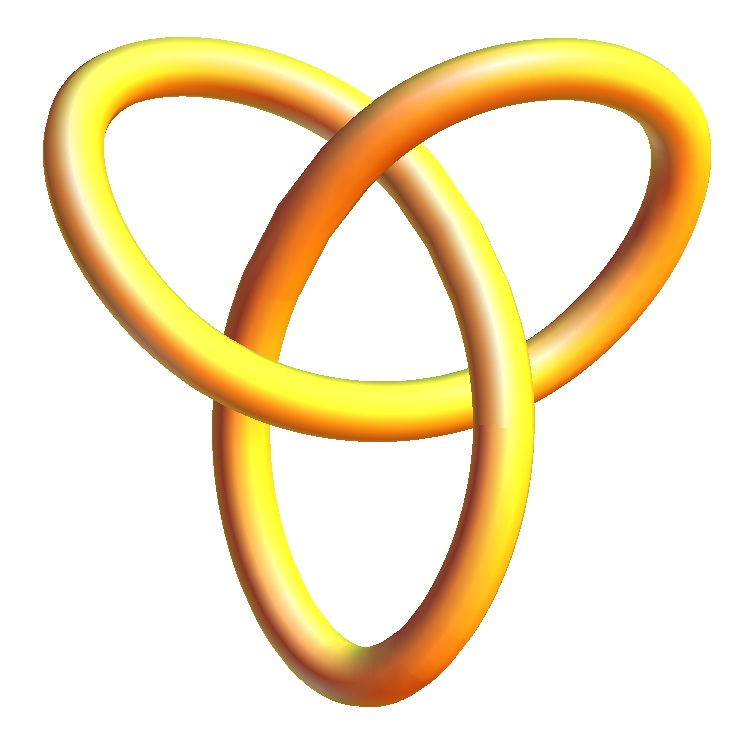
\includegraphics[scale=.333333]{Trefoil_Knot}}

\author{Michael N. Brown\\
  Brigham Young University}
\date{\today}
\maketitle

\tableofcontents

\part{Geometry}
Euclidean geometry is an axiomatic system, in which all theorems ("true statements") are derived from a small number of axioms.\footnote{The assumptions of Euclid are discussed from a modern perspective in Harold E. Wolfe (2007). Introduction to Non-Euclidean Geometry. Mill Press. p. 9. ISBN 1406718521.} Near the beginning of the first book of the Elements, Euclid gives five postulates (axioms) for plane geometry, stated in terms of constructions (as translated by Thomas Heath):\footnote{tr. Heath, pp. 195-202.}

"Let the following be postulated":
\begin{itemize}
\item[1.]"To draw a straight line from any point to any point."
\item[2.]"To produce [extend] a finite straight line continuously in a straight line."
\item[3.]"To describe a circle with any centre and distance [radius]."
\item[4.]"That all right angles are equal to one another."
\item[5.]The parallel postulate: "That, if a straight line falling on two straight lines make the interior angles on the same side less than two right angles, the two straight lines, if produced indefinitely, meet on that side on which are the angles less than the two right angles."
\end{itemize}
Although Euclid's statement of the postulates only explicitly asserts the existence of the constructions, they are also taken to be unique.

The Elements also include the following five "common notions":
\begin{itemize}
\item[1.]Things that are equal to the same thing are also equal to one another.
\item[2.]If equals are added to equals, then the wholes are equal.
\item[3.]If equals are subtracted from equals, then the remainders are equal.
\item[4.]Things that coincide with one another equal one another.
\item[5.]The whole is greater than the part.
\end{itemize}

\chapter{Geometric Formulas}
\section{2-dimensional Figures}

\subsection{Triangle}
\begin{tikzpicture}
\draw[->]
(0,0) -- (5,0) -- (5,5) -- cycle;
\draw[loosely dashed]
(0,0) -- +(0:1.5) arc(0:45:1.5) -- cycle;
\put(40, 80){\makebox(0, 0){$C (Hypotenuse)$}}
\put(80, -8){\makebox(0, 0){$A (Adjacent)$}}
\put(175, 80){\makebox(0, 0){$B(Opposite)$}}
\put(50, 22){\makebox(0, 0){$\theta$}}
\end{tikzpicture}\\\\
$Area=\frac{1}{2}BA=\frac{1}{2}CA\theta$

\subsection{Circle}
\begin{tikzpicture}
\draw[black,solid] (0,0) circle (3);
\multiput(0, 0)(0, 40){1}{\line(1, 0){86}}
\multiput(0, 0)(86, 0){2}{\circle*2}
\put(43, 5){\makebox(0, 0){$r$}}
\put(-20, 0){\makebox(0, 0){$(x_0, y_0)$}}
\put(100, 0){\makebox(0, 0){$(x,y)$}}
\end{tikzpicture}\\\\
$A=\pi r^2$\\
$C=2\pi r$

\subsection{Sector of Circle}
\begin{tikzpicture}
\draw[->]
(5,1) -- +(0:5) arc(0:45:5) -- cycle;
\draw[loosely dashed]
(5,1) -- +(0:1.5) arc(0:45:1.5) -- cycle;
\put(190, 90){\makebox(0, 0){$r$}}
\put(312, 90){\makebox(0, 0){$a=(Arc Length)$}}
\put(212, 21){\makebox(0, 0){$r=(Radius)$}}
\put(190, 47){\makebox(0, 0){$\theta$}}
\end{tikzpicture}\\\\
$A=\frac{1}{2}r^2\theta$\\
$a=r\theta$

\section{Cylinders}
A cylinder is a surface that consists of all lines that are parallel to a given line and pass through a given plane curve.

\subsection{Circular Cylinder}
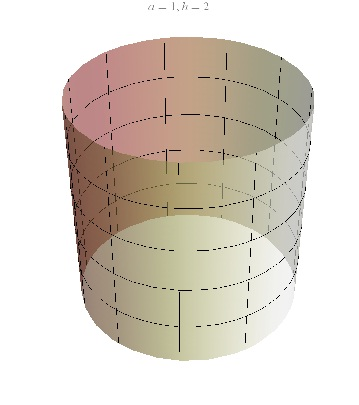
\includegraphics[scale=.5]{Circular_Cylinder}\\
$V=\pi r^2h$\\
An equation of a cylinder in $\mathbb{R}^3$ with the center of the base at the origin and radius $r$ is $x^2+y^2=r^2$ where the missing coordinate$(x,y,z)$ is the height.

\section{Quadric Surfaces}
A quadric surface is the graph of a second-degree equation in three variables $x,y,z$.\\
$\begin{array}{c c c}
&&\\
\textbf{Hyperboloid of One Sheet} & \textbf{Cone} & \textbf{Hyperboloid of Two Sheets}\\
x^2+y^2-z^2=1&x^2+y^2-z^2=0&x^2+y^2-z^2=-1\\
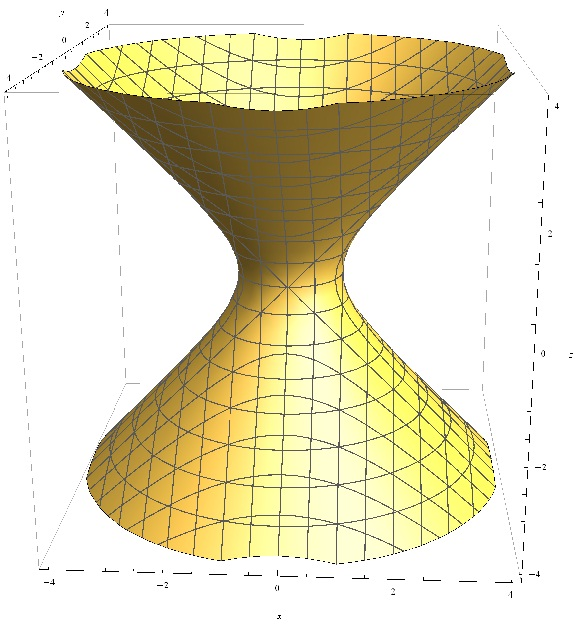
\includegraphics[scale=.333333]{Hyperboloid_One} & 
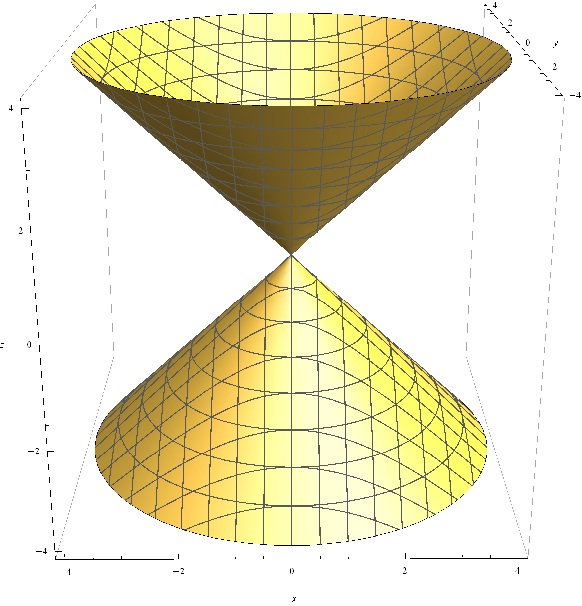
\includegraphics[scale=.333333]{cone} & 
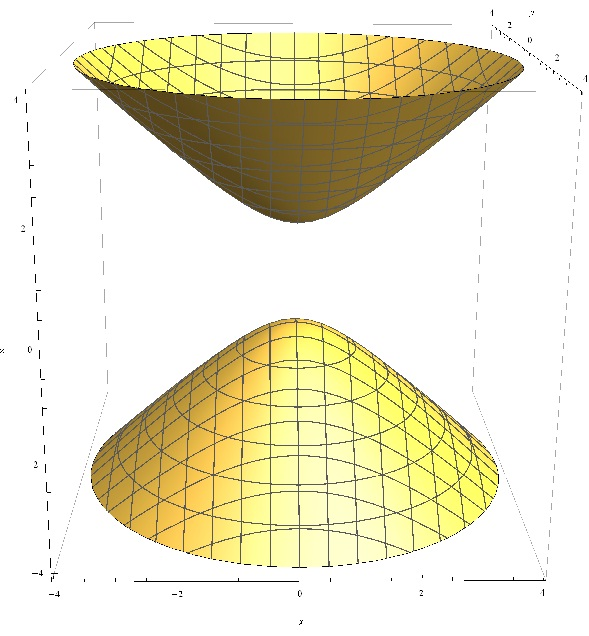
\includegraphics[scale=.333333]{Hyperboloid_Two}\\
&&\\

\textbf{Sphere} & 	\textbf{Ellipsoid}\\
x^2+y^2+z^2=1& \frac{x^2}{a} + \frac{y^2}{b} + \frac{z^2}{c} = 1\\
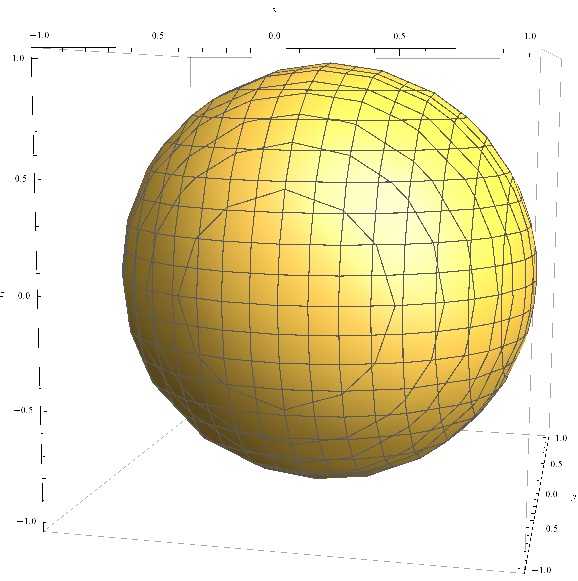
\includegraphics[scale=.333333]{sphere} &
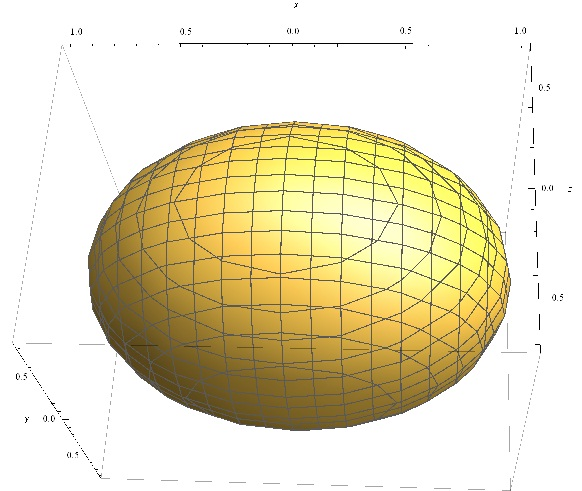
\includegraphics[scale=.333333]{Ellipsoid}\\
&&\\

\textbf{Elliptic Paraboloid} & 	\textbf{Hyperbolic Paraboloid}\\
x^2+y^2=z&x^2-y^2=z\\
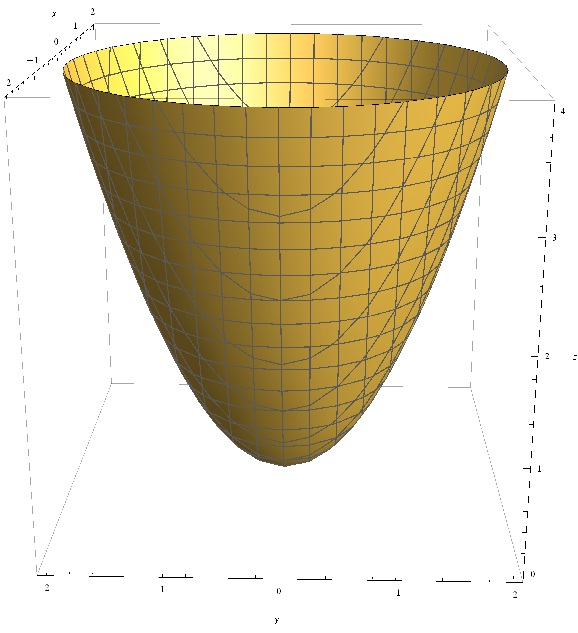
\includegraphics[scale=.333333]{Elliptic_Paraboloid} &
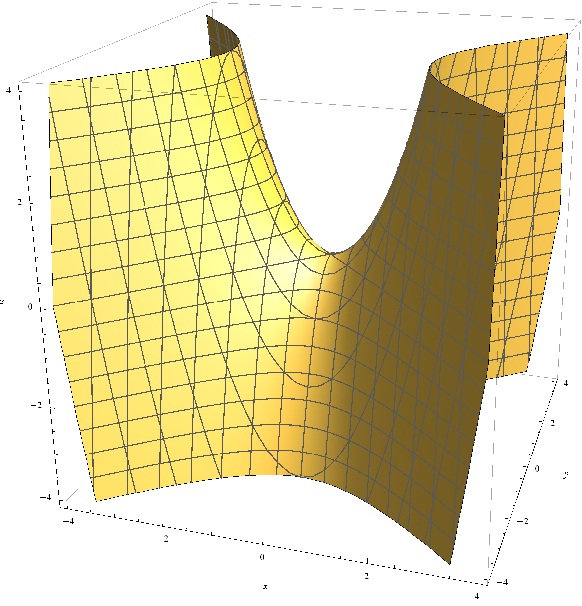
\includegraphics[scale=.333333]{Hyperbolic_Paraboloid}\\

\end{array}$
\chapter{Pythagorean Theorem}
\section{Theorem and Proof}
\begin{thm2}
$$a^2+b^2=c^2$$
\end{thm2}
\begin{proof}
Let's take two squares, one inside the other. The corners of the inside square intersect the sides of the outside square. We will assign the side lengths of the inside square each as $c$. The side lengths of the outside square will $a+b$ where $a$ and $b$ are on opposite sides of the intersection of the corner of square $c$ and side of square $ab$. This gives us 4 congruent triangles inside square $ab$ and outside square $c$. These 4 triangles, $\Delta abc$, have a base of $a$ and a height of $b$, with a hypotenuse of $c$.
We can compute the area of a square with side lengths $a + b$ using two methods:\\
\setlength{\unitlength}{1mm}
\begin{picture}(100,70)
\linethickness{1.5pt}
		% straight lines
		\multiput(20, 20)(0, 40){2}{\line(1, 0){40}}
                	\multiput(20, 20)(40, 0){2}{\line(0, 1){40}}
             	\multiput(20, 40)(20, -20){2}{\line(1, 1){20}}
            	\multiput(20, 40)(20, 20){2}{\line(1, -1){20}}
		% labels
		\put(28, 62){\makebox(0, 0){$a$}}
                	\put(18, 28){\makebox(0, 0){$a$}}
             	\put(62, 52){\makebox(0, 0){$a$}}
               	\put(52, 18){\makebox(0, 0){$a$}}
        		\put(28, 18){\makebox(0, 0){$b$}}
		\put(18, 52){\makebox(0, 0){$b$}}
      		\put(52, 62){\makebox(0, 0){$b$}}
  		\put(62, 28){\makebox(0, 0){$b$}}
		\put(28, 52){\makebox(0, 0){$c$}}
      		\put(28, 28){\makebox(0, 0){$c$}}
    		\put(52, 52){\makebox(0, 0){$c$}}
  		\put(52, 28){\makebox(0, 0){$c$}}
\end{picture}
\begin{itemize}
\item[1.] we can square the side lengths and
\item[2.] we can add the area of the 4 congruent triangles and then add them to the area of square $c$ which is $c^{2}$.  If we let A be the area of the square with side $a + b$, then calculating we have
\end{itemize}
\begin{itemize}
\item[Method 1:] $A = (a + b)^{2} = a^{2} + 2ab +b^{2}$
\item[Method 2:]  $A = 4(\frac{ab}{2}) + c^{2} = 2ab + c^{2}$
\end{itemize}
Methods 1 and 2 calculated the area of the same square, therefore they must be equal. This means that we can equate both expressions.  Equating we have,
$$a^{2} + 2ab + b^{2} = 2ab + c^{2} \to a^{2} + b^{2} = c^{2}$$
which is exactly what we want to show
\end{proof}
\begin{cor2}
If $a^{2} + b^{2} = c^{2}$, then the triangle is right.
\end{cor2}
\begin{cor2}
If $a^{2} + b^{2} > c^{2}$, then the triangle is acute.
\end{cor2}
\begin{cor2}
If $a^{2} + b^{2} < c^{2}$, then the triangle is obtuse.
\end{cor2}
\begin{cor2} 
$\textbf{The existence of irrational numbers.}$
One of the consequences of the Pythagorean theorem is that irrational numbers, such as $\sqrt{2}$, can be constructed. A right triangle with legs both equal to one unit has hypotenuse length $\sqrt{2}$. The Pythagoreans proved that the square root of 2 is irrational, and this proof has come down to us even though it flew in the face of their cherished belief that everything was rational. According to the legend, Hippasus, who first proved the irrationality of the square root of two, was drowned at sea as a consequence.
\end{cor2}
\begin{cor2} 
$\textbf{Distance in Cartesian coordinates}$ The distance formula in Cartesian coordinates is derived from the Pythagorean theorem. If $(x_1, y_1)$ and $(x_2, y_2)$ are points in the plane, then the distance between them, also called the Euclidean distance, is given by
$$\sqrt{(x_2-x_1)^2+(y_2-y_1)^2}$$
More generally, in Euclidean $n$-space, the Euclidean distance between two points, $A=(a_1,a_2,\dots,a_n)$ and $B=(b_1,b_2,\dots,b_n)$, is defined, using the Pythagorean theorem, as:
$$\sqrt{(a_1-b_1)^2+(a_2-b_2)^2+\dots +(a_n-b_n)^2}=\sqrt{\sum_{i=1}^n(a_i-b_i)^2}$$
\end{cor2}

\chapter{Lines and Planes}
\section{2-Dimensional Lines}
\subsection{Distance Formulas in 2, and N-dimensions}
Distance $|P_1P_2|$ where $P_1=(x_1, y_1)$ and $P_2=(x_2,y_2)$:
$$d=\sqrt{(x_2-x_1)^2+(y_2-y_1)^2}$$
Distance $|P_xP_y|$ where $P_x=(x_1, x_2,...,x_N)$ and $P_y=(y_1,y_2, ...,y_N)$:
$$d=\sqrt{(y_1-x_1)^2+(y_2-x_2)^2+ \cdots + (y_N-x_N)^2}$$
\subsection{Midpoint Formulas in 2, and N-dimensions}
Midpoints of $\overline{P_1P_2}$: $$\left(\frac{x_1+x_2}{2},\frac{y_1+y_2}{2}\right)$$
Midpoints of $\overline{P_xP_y}$: $$\left(\frac{x_1+y_1}{2},\frac{x_2+y_2}{2},\cdots\frac{x_N+y_N}{2}\right)$$
\subsection{Slope}
Slope of the line through $P_1(x_1,y_1)$ and $P_2(x_2,y_2)$:
$$m=\frac{y_2-y_1}{x_2-x_1}$$
\subsection{Point-slope Equation}
Point-slope equation of line through $P_1(x_1, y_1)$ with slope $m$:
$$y-y_1=m(x-x_1)$$
\subsection{Slope-Intercept}
Slope-intercept equation of the line with slope $m$ and $y$-intercept $b$:
$$(x-h)^2+(y-k)^2=r^2$$
\section{Vectors and Vector Functions}
A displacement vector $\vec{v}$ has an initial point $A$ and a terminal point $B$  and we indicate this by writing $\vec{v}=\vec{AB}$
\subsection{Vector Equation}
In three-dimensions the direction of a line is conveniently described by a vector, so we let $v$ be a vector parallel to $L$. Let $P(x,y,z)$ be an arbitrary point on $L$ and let $r_0$ and $r$ be the position vectors of $P_0$ and $P$ (that is they have representations $\vec{OP_0}$ and $\vec{OP}$). If $a$ is the vector with representation $\vec{P_0P}$, then the Triangle Law for vector addition gives $r = r_0 + a$. But since $a$ and $v$ are parallel vectors, there is a scalar $t$ such that $a=tv$. Thus
$$r = r_0 + tv$$
\subsection{Parametric Equations}
Each value of the parameter $t$ gives the position vector $r$ of a point on $L$. If the vector $v$ that gives the direction of the line $L$ is written in component form as $v=\langle a,b,c\rangle$, then we have $tv=\langle ta,tb,tc\rangle$. We can also write $r=\langle x,y,z\rangle$ and $r_0=\langle x_0,y_0,z_0\rangle$. So the vector equation becomes
$$\langle x,y,z\rangle = \langle x_0 + ta, y_0 + tb, z_0 + tc\rangle$$
The two vectors are equal if and only if corresponding components are equal. Therefore we have three scalar equations
$$x = x_0 + at, y= y_0 + bt, z = z_0 + ct$$
\subsection{Continuity}
\begin{def3}[Limit]
The limit of a vector function $\vec{r}$ is defined by taking the limits of its component functions as follows
If $\vec{r}(t) = \langle f(t), g(t) ,h(t) \rangle$ then
$$ \lim_{t\to a} \vec{r}(t) = \langle \lim_{t\to a} f(t),\lim_{t\to a} g(t), \lim_{t\to a} h(t) \rangle$$
provided the limits of the component functions exist.
\end{def3}
\begin{def3}[Continuous]
A vector function $\vec{r}$ is continuous at $a$ if
$$\lim_{t\to a} \vec{r}(t) = \vec{r}(a)$$
\end{def3}
\subsection{Arc Length}
\begin{def3}[Arc Length Function]
Suppose that the curve has the vector equation $\vec{r}(t) = \langle f(t), g(t), h(t) \rangle, a\leq t \leq b$, or, equivalently, the parametric equations $x=f(t), y=g(t), z=h(t)$, where $f',g',h'$ are continuous. If the curve is traversed exactly once as $t$ increases from $a$ to $b$, then its length is 
$$L = \int_a^b \sqrt{[f'(t)]^2+[g'(t)]^2+[h'(t)]^2}dt = \int_a^b \sqrt{\left(\frac{dx}{dt}\right)^2+\left(\frac{dy}{dt}\right)^2+\left(\frac{dz}{dt}\right)^2}dt$$
or
$$s(t) = \int_a^t ||\vec{r}'(u)||du$$
Thus $s(t)$ is the length of the curve from $r(a)$ to $r(t)$. If we differentiate each side and use Part 1 of the Fundamental Theorem of Calculus, we get
$$\frac{ds}{dt}=||\vec{r}'(t)||$$
\end{def3}
\subsection{Curvature}
\begin{def3}[Unit Tangent Vector]
A parametrization $\vec{r}(t)$ is called smooth on an interval $I$ if $\vec{r}'$ is continuous and $\vec{r}'(t)\neq 0$ on $I$. A curve is smooth if it has a smooth parametrization. A smooth curve has no sharp corners or cusps.
If a curve $C$ is a smooth curve defined by the vector $\vec{r}$, the unit tangent vector $\vec{T}(t)$ is given by
$$\vec{T}(t) = \frac{\vec{r}'(t)}{||\vec{r}'(t)||}$$
and indicates the direction of the curve.
\end{def3}
\begin{def3}[Curvature]
The curvature of a curve is
$$\kappa = \left|\left|\frac{d\vec{T}}{ds}\right|\right|$$
where $\vec{T}$ is the unit tangent vector.
$$\frac{d\vec{T}}{dt}=\frac{d\vec{T}}{ds}\frac{ds}{dt} \text{  and  } \kappa = \left|\left|\frac{d\vec{T}}{ds}\right|\right| = \left|\left|\frac{\frac{d\vec{T}}{dt}}{\frac{ds}{dt}}\right|\right|$$
but $\frac{ds}{dt}=||\vec{r}'(t)||$, so
$$\kappa(t) = \frac{||\vec{T}'(t)||}{||\vec{r}'(t)||}$$
\end{def3}
\begin{thm3}
The curvature of the curve given by the vector function $\vec{r}$ is
$$\kappa (t) = \frac{||\vec{r}'(t) \times \vec{r}''(t)||}{||\vec{r}'(t)||^3}$$
\end{thm3}
\begin{proof}
Since $\vec{T}=\frac{\vec{r}'}{||\vec{r}'||}$ and $||\vec{r}'|| = \frac{ds}{dt}$, we have 
$$\vec{r}' = ||\vec{r}'||\vec{T} = \frac{ds}{dt}\vec{T}$$
so the product rule gives us
$$\vec{r}'' = \frac{d^2s}{dt^2}\vec{T} + \frac{ds}{dt}\vec{T}'$$
Using the fact that $\vec{T}\times \vec{T} = \vec{0}$, we have
$$\vec{r}' \times \vec{r}'' = \left( \frac{ds}{dt}\right) ^2 (\vec{T}\times \vec{T}')$$
Now $||\vec{T}(t)|| = 1, \forall t$, so $\vec{T}$ and $\vec{T}'$ are orthogonal.
$$||\vec{r}' \times \vec{r}''|| = \left( \frac{ds}{dt}\right) ^2 ||\vec{T}\times \vec{T}'|| = \left( \frac{ds}{dt}\right) ^2 ||\vec{T}||||\vec{T}'|| = \left( \frac{ds}{dt}\right) ^2 ||\vec{T}'||$$
Thus
$$||\vec{T}'|| = \frac{||\vec{r}'\times \vec{r}''||}{(ds/dt)^2} = \frac{||\vec{r}' \times \vec{r}''||}{||\vec{r}||^2}$$
and
$$\kappa = \frac{||\vec{T}'||}{||\vec{r}'||} = \frac{||\vec{r}' \times \vec{r}''||}{||\vec{r}'||^3}$$ 
\end{proof}
\section{Planes}
Although a line in space is determined by a point and a direction, a plane in space is more difficult to describe. A single vector parallel to a plane is not enough to convey the "direction" of the plane, but a vector perpendicular to the plane does completely specify its direction. Thus a plane in space is determined by a point $P_0(x_0, y_0, z_0)$ in the plane and a vector $\vec{n}$, known as the normal vector,  that is orthogonal to the plane. 
\begin{def2}[Vector Equation of a Plane]
Let $P(x,y,z)$ be an arbitrary point in the plane, and let $\vec{r}_0$ and $\vec{r}$ be the position vectors of $P_0$ and $P$. Then the vector $\vec{r}-\vec{r}_0$ is represented by $\vec{P_0P}$. The normal vector $\vec{n}$ is orthogonal to $\vec{r}-\vec{r}_0$ and so we have
$$\vec{n}\cdot (\vec{r}-\vec{r}_0)= 0$$
which can be rewritten as
$$\vec{n}\cdot \vec{r} = \vec{n} \cdot \vec{r}_0$$
\end{def2}
\begin{def2}[Scalar Equation of the Plane]
Let $\vec{n}=\langle a,b,c\rangle, \vec{r} = \langle x,y,z\rangle$, and $\vec{r}_0 = \langle x_0, y_0, z_0\rangle$. Then the vector equation becomes
$$\langle a,b,c\rangle \cdot \langle x-x_0, y-y_0, z-z_0\rangle = 0$$
or
$$a(x-x_0) + b(y-y_0) + c(z-z_0) = 0$$
\end{def2}
\begin{def2}[Parallel Planes]
Two planes are parallel if their normal vectors are parallel
\end{def2}
\section{The Normal and Binormal Vectors}
\begin{def2}[Unit Tangent Vector]
$$\vec{T}(t) = \frac{\vec{r}'(t)}{||\vec{r}'(t)||}$$
\end{def2}
\begin{def2}[The Principal Unit Normal Vector]
$$\vec{N} = \frac{\vec{T}'}{||\vec{T}'||}$$
\end{def2}
\begin{def2}[The Binormal Vector]
$$\vec{B} = \vec{T}(t)\times\vec{N}(t)$$
\end{def2}
\begin{def2}[The Normal Plane]
The plane determined by the normal and binormal vectors $\vec{N}$ and $\vec{B}$ at a point $P$ on a curve $C$ is called the normal plane of $C$ at $P$. It consists of all lines that are orthogonal to the tangent vector $\vec{T}$. 
\end{def2}
\begin{def2}[Osculating Plane]
The plane determined by the vectors $\vec{T}$ and $\vec{N}$ is called the osculating plane of $C$ at $P$. It is the plane that comes closest to containing the part of the curve near $P$. (For a plane curve, the osculating plane is simply the plane that contains the curve.)
\end{def2}
\section{Tangential and Normal Components of Acceleration}
When we study the motion of a particle, it is often useful to resolve the acceleration into two components, one in the direction of the tangent and the other in the direction of the normal.
$$\vec{a} = a_T\vec{T} + a_N\vec{N}$$
Where
$$a_T = \frac{\vec{r}'(t) \cdot \vec{r}''(t)}{||\vec{r}'(t)||}$$
$$a_N = \frac{||\vec{r}'(t) \times \vec{r}'' (t)||}{||\vec{r}'||}$$

\part{Trigonometry}
\chapter{Unit Circle}
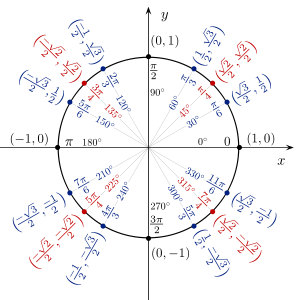
\includegraphics[scale=.75]{Unit_circle_angles_color}\\
If $(x, y)$ is a point on the unit circle in the first quadrant, then $x$ and $y$ are the lengths of the legs of a right triangle whose hypotenuse has length $1$. Thus, by the Pythagorean theorem, $x$ and $y$ satisfy the equation
$$x^2+y^2=1$$
Since $x^2 = (-x)^2$ for all $x$, and since the reflection of any point on the unit circle about the $x$-axis or $y$-axis is also on the unit circle, the above equation holds for all points $(x, y)$ on the unit circle, not just those in the first quadrant.

\section{Formulas Derived from the Pythagorean Theorem and Unit Circle}
\subsection{Definitions}
\begin{thm3}$\sin\theta = \cos(\frac{\pi}{2} - \theta)$\end{thm3}
\begin{thm3}$\cos\theta = \sin (\frac{\pi}{2} - \theta)$\end{thm3}
\begin{thm3}$\tan \theta = \frac{\sin\theta}{\cos \theta} = \frac{1}{\cot \theta}$ \end{thm3}
\begin{thm3}$\csc\theta = \frac{1}{\sin\theta}$\end{thm3}
\begin{thm3}$\sec\theta = \frac{1}{\cos\theta}$\end{thm3}
\begin{thm3}$\cot\theta = \frac{\cos\theta}{\sin \theta} = \frac{1}{\tan\theta}$ \end{thm3}
\subsection{Double Angle Formulas}
\begin{thm3}$\sin2\theta = 2\sin\theta\cos\theta$\end{thm3}
\begin{thm3}$\cos2\theta =\cos^{2}\theta - \sin^{2}\theta = 2\cos^{2}\theta - 1 = 1 - 2\sin^{2}\theta$\end{thm3}
\begin{thm3}$\tan2\theta = \frac{2\tan\theta}{1 - \tan^{2}\theta}$\end{thm3}
\subsection{Half-angle Formulas}
\begin{thm3}$\sin^{2}\theta = \frac{1 - \cos2\theta}{2}$\end{thm3}
\begin{thm3}$\cos^{2}\theta = \frac{1 + \cos2\theta}{2}$\end{thm3}
\subsection{Pythagorean Identities}
\begin{thm3}$\sin^{2}\theta + \cos^{2}\theta=1$\end{thm3}
\begin{thm3}$1 + \tan^{2}\theta = \sec^{2}\theta$\end{thm3}
\begin{thm3}$1 + \cot^{2}\theta = \csc^{2}\theta$\end{thm3}
\subsection{Reduction Formulas}
\begin{thm3}$\sin(- \theta) = - \sin \theta$\end{thm3}
\begin{thm3}$\cos(-\theta) = \cos \theta$\end{thm3}
\begin{thm3}$\tan(- \theta) = -\tan \theta$\end{thm3}
\subsection{Summation and Difference Formulas}
\begin{thm3}$\sin(A + B) = \sin A\cos B + \sin B\cos A$\end{thm3}
\begin{thm3}$\tan(A+B)=\frac{\tan A+\tan B}{1-\tan A\tan B}$\end{thm3}
\begin{thm3}$\sin(A - B)=\sin A\cos B-\sin B\cos A$\end{thm3}
\begin{thm3}$\cos(A + B)=\cos A\cos B- \sin B\sin A$\end{thm3}
\begin{thm3}$\tan(A-B)=\frac{\tan A- \tan B}{1+\tan A\tan B}$\end{thm3}
\begin{thm3}$\cos(A - B)=\cos A\cos B+\cos B\cos A$\end{thm3}
\subsection{Inverse Trigonometric Functions}
\begin{thm3}$\sin^{-1} \theta = y \iff \sin y = \theta\text{, }-\frac{\pi}{2} \leq y \leq \frac{\pi}{2}$\end{thm3}
\begin{thm3}$\sin^{-1}(\sin\theta) = \theta \text{,  }- \frac{\pi}{2} \leq \theta \leq \frac{\pi}{2}$\end{thm3}
\begin{thm3}$\sin(\sin^{-1} \theta) = \theta\text{, }-1 \leq \theta \leq 1$\end{thm3}
\begin{thm3}$\cos^{-1} \theta = y \iff \cos y = \theta\text{, }0 \leq y \leq \pi$\end{thm3}
\begin{thm3}$\cos^{-1}(\cos \theta) = \theta\text{, }0 \leq \theta \leq \pi$\end{thm3}
\begin{thm3}$\cos(\cos^{-1} \theta) = \theta\text{, }-1 \leq \theta \leq 1$\end{thm3}
\begin{thm3}$\tan^{-1} \theta = y \iff \tan y = \theta\text{, }-\frac{\pi}{2} \leq y \leq \frac{\pi}{2}$\end{thm3}
\begin{thm3}$y = \csc^{-1} \theta\text{, }(| \theta | \geq 1) \iff \csc y = \theta\text{, }y \in \left(0, \frac{\pi}{2}\right] \cup \left(\pi, \frac{3 \pi}{2}\right]$\end{thm3}
\begin{thm3}$y = \sec^{-1} \theta\text{, }(| \theta | \geq 1) \iff \sec y = \theta\text{, }y \in \left[0, \frac{\pi}{2}\right) \cup \left[\pi, \frac{3 \pi}{2}\right)$\end{thm3}
\begin{thm3}$y = \cot^{-1} \theta\text{, }(| \theta | \in \mathbb{R}) \iff \cot y = \theta\text{, }y \in (0,\pi)$\end{thm3}
\begin{thm3}$\sinh^{-1}=\ln (x+\sqrt{x^2+1}), x\in\mathbb{R}$\end{thm3}
\begin{thm3}$\cosh^{-1}=\ln (x+\sqrt{x^2-1}), x\geq 1$\end{thm3}
\begin{thm3}$\tanh^{-1}=\frac{1}{2}\ln \left(\frac{1+x}{1-x}\right), -1<x<1$\end{thm3}
\part{Calculus}
The functions encountered in calculus are real-valued functions defined on sets of real numbers. That is, each function that we study in calculus is of the type $f: X\to \mathbb{R}$, where $X\subseteq\mathbb{R}$. In the study of limits, we are often interested in such functions having the property that either $(1)X= \mathbb{N}$ and increasing values in the domain $\mathbb{N}$ result in functional values approaching some real number $L$, or (2) the function is defined for all real numbers near some specified real number $a$ and values approaching $a$ result in functional values approaching some real number $L$.

\chapter{Infinite Sequences and Series}
\section{Rearrangements of Infinite Sets}
\section{The Limit of a Sequence}
\begin{def2}[Sequence]
A sequence of real numbers is a real-valued function defined on the set of natural numbers; that is, a sequence is a function $f:\mathbb{N}\to \mathbb{R}$. If $f(n)=a_n, \forall n\in \mathbb{N}$, then $f = \{(1,a_1),(2,a_2),(3,a_3),...\}$. Since only the numbers $a_1, a_2, a_3,...$ are relevant in $f$, we also refer to $a_1, a_2, a_3,...$ as the sequence, which we often denote by $\{a_n\}$. The numbers $a_1, a_2, a_3,...$ are called the terms of $\{a_n\}$, with $a_1$ being the first term, $a_2$ the second term, etc. Thus $a_n$ is the $n$th term of the sequence.
\end{def2}
\begin{def2}[Limit of a Sequence]
For some sequences $\{a_n\}$, there is a real number $L$ (or at least there appears to be a real number $L$) such that the larger the integer $n$ becomes, the closer $a_n$ is to $L$. \\
A sequence $\{a_n\}$ is said to converge to a real number $L$ if the larger the integer $n$, the closer $a_n$ is to $L$.\\
What we want to say then is that we can make $a_n$ as close to $L$ as we wish (that is, we can make $|a_n - L|$ as small as we wish) provided that $n$ is large enough. Let $\eps$ denote how small we want $|a_n-L|$ to be; that is, we want $|a_n-L|<\eps$ by choosing $n$ large enough. This is equivalent to $-\eps<a_n-L<\eps$, that is, $L-\eps <a_n<L+\eps$. Hence we require that $a_n$ be a number in the open interval $(L-\eps,L+\eps)$ when $n$ is large enough. So there exists $N\in \mathbb{N}$ such that if $n$ is an integer greater than $N$, then $a_n\in (L-\eps, L+\eps)$. If such a positive integer $N$ can be found for every positive number $\eps$, regardless of how small $\eps$ might be, then we say that $\{a_n\}$ converges to $L$.\\\\

If a sequence $\{a_n\}$ has limit $L$ then we write
$$\lim_{n\to \infty} a_n = L \text{   or   } a_n \to L \text{ as } n\to \infty$$
$$\forall \eps > 0 \exists N\in\mathbb{N} \ni n>N\implies |a_n - L| < \eps$$\\
Consequently, if a sequence $\{a_n\}$ does not converge it is said to diverge and there is no real number $L$ such that $\lim_{n\to \infty} a_n=L$
To prove that a sequence $\{a_n\}$ diverges, a proof by contradiction would be anticipated. We would begin such a proof by assuming, to the contrary, that $\{a_n\}$ converges, say to some real number $L$. We know $\forall \eps >0 \exists N\in \mathbb{N}\ni \forall n>N\implies |a_n-L|<\eps$. Show contradiction.
\end{def2}

\begin{def2}[Convergence of a Sequence]
A sequence $(a_n)$ converges to a real number $a$ if, for every positive number number $\eps$, there exists an $N\in\mathbb{N}$ such that whenever $n\geq N$ it follows that $|a_n-a|<\eps$
\end{def2}
\begin{def2}
Given a real number $a\in \mathbb{R}$ and a positive number $\eps >0$, the set
$$V_\eps(a) = \{x\in\mathbb{R}:|x-a|<\eps\}$$
is called the $\eps$-neighborhood
\end{def2}
\begin{def2}
Learning to write a grammatically correct convergence proof goes hand in hand with a deep understanding of why the quantifiers appear in the order with the phrase,
$$\forall \eps, \exists N\in\mathbb{N}\ni...$$
TEMPLATE FOR A PROOF THAT $(x_n)\to x$
\begin{itemize}
\item[-] "Let $\eps>0$ be arbitrary"
\item[-] Demonstrate a choice for $N\in \mathbb{N}$. This step usually requires the most work, almost all of which is done prior to actually writing the formal proof.
\item[-] Now, show that $N$ actually works
\item[-] "Assume $n\geq N$"
\item[-] With $N$ well chosen, it should be possible to derive the inequality $|x_n-x|<\eps$
\end{itemize}
\end{def2}
\begin{def2}
A sequence that does not converge is said to diverge
\end{def2}
\section{The Algebraic and Order Limit Theorem}
\begin{def2}
A sequence $(x_n)$ is bounded if there exists a number $M>0$ such that $|x_n|\leq M$ for all $n\in \mathbb{N}$
\end{def2}
\begin{thm2}
Every convergent sequence is bounded
\end{thm2}
\begin{proof}
Assume $(x_n)$ converges to a limit $l$. This means that given a particular value of $\eps$, say $\eps =1$, we know there must exist an $N\in\mathbb{N}$ such that if $n\geq N$, then $x_n$ is in the interval $(l-1,l+1)$. Not knowing whether $l$ is positive or negative, we can certainly conclude that
$$|x_n|<|l|+1$$
for all $n\geq N$.
We still need to worry (slightly) about the terms in the sequence that come before the $N$th term. Because there are only a finite number of these, we let
$$M = \max\{|x_1|,|x_2|,|x_3|,...,|x_{N-1}|, |l|+1\}$$
It follows that $|x_n|\leq M$ for all $n\in\mathbb{N}$, as desired.
\end{proof}
\begin{thm2}[Algebraic Limit Theorem for Sequences]
Let $\lim a_n = a$, and $\lim b_n = b$. Then
\begin{itemize}
\item[(i)]$$\lim_{n\to \infty} (a_n + b_n) = a + b$$
\item[(ii)]$$\lim_{n\to \infty} (a_n - b_n) = a - b$$
\item[(iii)]$$\lim_{n\to \infty} ca_n = ca$$
\item[(iv)]$$\lim_{n\to \infty} (a_nb_n) = ab$$
\item[(v)]$$\lim_{n\to \infty} \frac{a_n}{b_n} = \frac{a}{b}$$
\item[(vi)]$$\lim_{n\to \infty} a_n^p = \left[ \lim_{n\to \infty}a_n\right]^p \text{ if } p>0 \text{ and } a_n>0$$
\item[(vii)] If $\lim_{n\to \infty} a_n=L$ and the function $f$ is continuous at $L$, then
$$\lim_{n\to \infty} f(a_n) = f(L)$$
\item[(viii)] The sequence $\{r^n\}$ is convergent if $-1<r\leq 1$ and divergent for all other values of $r$.
$$\lim_{n\to \infty} r^n = \begin{cases}
0, & -1<r< 1\\
1, & r=1
\end{cases}$$
\end{itemize}
\end{thm2}
\begin{proof}
\begin{itemize}
\item[(i)] *****
\item[(ii)] *****
\item[(iii)] *****
\item[(iv)] *****
\item[(v)] *****
\item[(vi)] *****
\item[(vii)] *****
\item[(viii)] *****
\end{itemize}
\end{proof}
\section{The Monotone Convergence Theorem and a First Look at Infinite Series}
\begin{def2}[Increasing, Decreasing, Monotonic]
A sequence $\{a_n\}$ is called increasing if $a_n < a_{n+1}\forall n\geq 1$. It is called decreasing if $a_n > a_{n+1}\forall n\geq 1$. A sequence is monotonic if it is either increasing or decreasing.
\end{def2}
\begin{thm2}[Monotonic Sequence Theorem]
Every bounded, monotonic sequence is convergent
\end{thm2}
\begin{proof}
Suppose $\{a_n\}$ is an increasing sequence. Since $\{a_n\}$ is bounded, the set $S=\{a_n:n\geq 1\}$ has an upper bound. By the Completeness Axiom it has a least upper bound $L$. Given $\eps>0, L-\eps$ is not an upper bound for $S$ (since $L$ is the least upper bound). Therefore
$$\exists N\in\mathbb{N}\ni a_N> L-\eps$$
\end{proof}

\section{Subsequences and the Bolzano-Weierstrass Theorem}
\begin{def2}
Let $(a_n)$ be a sequence of real numbers, and let $n_1<n_2<n_3<n_4<n_5<\cdots$ be an increasing sequence of natural numbers. Then the sequence
$$a_{n_1},a_{n_2},a_{n_3},a_{n_4},a_{n_5},\cdots$$
is called a subsequence of $(a_n)$ and is denoted by $(a_{n_j})$, where $j\in\mathbb{N}$ indexes the subsequence.
\end{def2}
\begin{thm2}
Subsequences of a convergent sequence converge to the same limit as the original sequence.
\end{thm2}
\begin{proof}
*****
\end{proof}
\begin{thm2}[The Bolzano-Weierstrass Theorem]
Every bounded sequence contains a convergent subsequence.
\end{thm2}
\begin{proof}
Let $(a_n)$ be a bounded sequence so that there exists $M>0$ satisfying $|a_n|\leq M, \forall n\in\mathbb{N}$.Bisect the closed interval $[-M,M]$ into the two closed intervals $[-M,0]$ and $[0,M]$. (The midpoint is included in both halves.) Now, it must be that at least one of these closed intervals contains an infinite number of the points in the sequence $(a_n)$. Select a half for which this is the case and label that interval as $I_1$. Then, let $a_{n_1}$ be some point in the sequence $(a_n)$ satisfying $a_{n_1}\in I_1$ *****
\end{proof}
\section{The Cauchy Criterion}
\begin{def2}[Cauchy Sequence]
A sequence $(a_n)$ is called a Cauchy sequence if, for every $\eps>0, \exists N\in\mathbb{N}\ni m,n\geq N\implies |a_n - a_m|<\eps$.
\end{def2}
\begin{def2}[Convergence of a Sequence]
A sequence $(a_n)$ converges to a real number $a$ if, for every $\eps>0$, there exists an $N\in\mathbb{N}$ such that whenever $n\geq N$ it follows that $|a_n-a|<\eps$.
\end{def2}
\begin{thm2}
Every convergent sequence is a Cauchy sequence.
\end{thm2}
\begin{proof}
Assume $(x_n)$ converges to $x$. To prove that $(x_n)$ is Cauchy, we must find a point in the sequence after which we have $|x_n-x_m|<\eps$. This can be done using an application of the triangle inequality.\\
*****
\end{proof}
\begin{lem2}
Cauchy sequences are bounded.
\end{lem2}
\begin{proof}
Given $\eps=1$, there exists an $N$ such that $|x_m-x_n|<1$ for all $m,n\geq N$. Thus, we must have $|x_n|<|x_N|+1$ for all $n\geq N$. It follows that
$$M=\max\{|x_1|,|x_2|,|x_3|,...,|x_{N-1}|,|x_N|+1\}$$
is a bound for the sequence $(x_n)$
\end{proof}
\begin{thm2}[Cauchy Criterion]
A sequence converges if and only if it is a Cauchy sequence.
\end{thm2}
\begin{proof}
$(\Rightarrow)$\\
$(\Leftarrow)$*****
\end{proof}
\section{Properties of Infinite Series}
\begin{def2}
For real numbers $a_1, a_2, a_3,...,$ we write $\sum_{k=1}^\infty a_k = a_1 + a_2 + a_3 + \cdots$ to denote an infinite series. The notation certainly seems to suggest that we are adding the terms $a_1, a_2, a_3,...$. But what does it mean to add infinitely many numbers? A meaning must be given to this. For this reason, we construct a sequence $\{s_n\}$, called the sequence of partial sums of the series. Here $s_1=a_1, s_2 = a_1+a_2,s_3 = a_1 + a_2 + a_3$, and in general, for $n\in \mathbb{N}$
$$s_n = a_1 + a_2 + \cdots + a_n = \sum_{k=1}^\infty a_k$$
Because $s_n$ is determined by adding a finite number of terms, there is no confusion in understanding the terms of the sequence $\{s_n\}$. If the sequence $\{s_n\}$ converges, say to the number $L$, then the series $\sum_{k=1}^\infty a_k$ is said to converge to $L$ and we write $\sum_{k=1}^\infty a_k = L$. This number $L$ is called the sum of $\sum_{k=1}^\infty a_k = L$. If $\{s_n\}$ diverges, then $\sum_{k=1}^\infty a_k = L$ is said to diverge.
\end{def2}
\begin{def2}[Geometric Series]
The geometric series
$$\sum_{n=1}^\infty ar^{n-1} = a + ar + ar^2 + \cdots$$
is convergent if $|r|<1$ and its sum is
$$\sum_{n=1}^\infty ar^{n-1} = \frac{a}{1-r}, |r|<1$$
If $|r|\geq 1$, the geometric series is divergent.
\end{def2}
\begin{def2}[Telescoping Series]
Written as partial sums, with the middle terms cancelling. Because of all of the cancelling, the sum collapses.
\end{def2}
\begin{thm2}[Test for Divergence]
 If $\lim_{n\to \infty}a_n$ does not exist or if $\lim_{n\to \infty}a_n \neq 0$, then the series $\sum_{n=1}^\infty a_n$ is divergent. 
\end{thm2}
Note: If we find that $\lim_{n\to \infty} a_n \neq 0$, we know that $\sum a_n$ is divergent. If we find that $\lim_{n\to \infty} a_n = 0$, we know nothing about the convergence or divergence of $\sum a_n$.
\begin{thm2}
If the series $\sum_{n=1}^\infty a_n$ is convergent, then $\lim_{n\to \infty} a_n =0$
Note: The converse is not true in general. If $\lim_{n\to \infty} a_n \neq 0$, we cannot conclude that $\sum a_n$ is convergent.
\end{thm2}
\begin{proof}
Let $s_n = a_1 + a_2 + \cdots + a_n$. Then $a_n = s_n - s_{n-1}$. Since $\sum a_n$ is convergent, the sequence $\{s_n\}$ is convergent. Let $\lim_{n\to \infty}s_n = s$. Since $n-1\to \infty$ as $n\to \infty$, we also have $\lim_{n\to \infty}s_{n-1}=s.$ Therefore,
$$\lim_{n\to \infty}a_n = \lim_{n\to \infty} (s_n-s_{n-1}) = \lim_{n\to\infty}s_n - \lim_{n\to \infty} s_{n-1} = s - s =0$$
\end{proof}
Note: With any series $\sum a_n$ we associate two sequences: the sequence $\{s_n\}$ of its partial sums and the sequence $\{a_n\}$ of its terms. If $\sum a_n$ is convergent, then the limit of the sequence $\{s_n\}$ is $s$ (the sum of the series) and the limit of the sequence $\{a_n\}$ is 0.
\begin{thm2}
If $\sum a_n$ and $\sum b_n$ are convergent series, then so are the following:
\begin{itemize}
\item[(i)] $$\sum_{n=1}^\infty ca_n = c\sum_{n=1}^\infty a_n$$
\item[(ii)] $$\sum_{n=1}^\infty (a_n + b_n)= \sum_{n=1}^\infty a_n + \sum_{n=1}^\infty b_n$$
\item[(iii)] $$\sum_{n=1}^\infty (a_n - b_n)= \sum_{n=1}^\infty a_n - \sum_{n=1}^\infty b_n$$
\end{itemize}
\end{thm2}
\begin{proof}
Proof is analogous to limit laws
\end{proof}
\subsection{Convergence and Divergence Tests and Estimates of Sums}
\begin{thm2}[The Integral Test]
Suppose $f$ is a continuous function, positive, decreasing function on $[1, \infty)$ and let $a_n = f(n)$. Then the series $\sum_{n=1}^\infty a_n$ is convergent if and only if the improper integral $\int_1^\infty f(x)dx$ is convergent.
\begin{itemize}
\item[(i)] If $\int_1^\infty f(x)dx$ is convergent, the $\sum_{n=1}^\infty a_n$ is convergent
\item[(ii)] If $\int_1^\infty f(x)dx$ is divergent, the $\sum_{n=1}^\infty a_n$ is divergent
\end{itemize}
\end{thm2}
Note: When we use the Integral Test, it is not necessary to start the series or the integral at $n=1$. In order to use the Integral Test we need to be able to evaluate $\int_1^\infty f(x)dx$ and therefore we have to be able to find an anti-derivative of $f$. Frequently this is difficult or impossible, so we need other tests for convergence too.
\begin{thm2}[$p$-series]
The $p$-series $\sum_{n=1}^\infty \frac{1}{n^p}$ is convergent if $p>1$ and divergent if $p\leq 1$
\end{thm2}
Note: We should not infer from the Integral Test that the sum of the series is equal to the value of the integral.
\begin{thm2}[Remaining Estimate for the Integral Test]
Suppose $f(k) = a_k$, where $f$ is a continuous, positive, decreasing function for $x\geq n$ and $\sum a_n$ is convergent. If $R_n = s- s_n$, then
$$\int_{n+1}^\infty f(x)dx \leq R_n \leq \int_n^\infty f(x)dx$$
If we add $s_n$ to each side of the inequality, we get
$$s_n + \int_{n+1}^\infty f(x)dx \leq s \leq s_n + \int_n^\infty f(x)dx$$
\end{thm2}
\begin{thm2}[The Comparison Test]
Suppose the $\sum a_n$ and $\sum b_n$ are series with positive terms.
\begin{itemize}
\item[(i)] If $\sum b_n$ is convergent and $a_n\leq b_n, \forall n \implies \sum a_n$ is also convergent
\item[(ii)] If $\sum b_n$ is divergent and $a_n\geq b_n, \forall n \implies \sum a_n$ is also divergent
\end{itemize}
\end{thm2}
\begin{proof}
Let
$$\begin{array}{c c c} 
s_n = \sum_{i=1}^n a_i & t_n = \sum_{i=1}^n b_i & t = \sum_{i=1}^\infty b_n
\end{array}$$
\begin{itemize}
\item[(i)] Since both series have positive terms, the sequences $\{s_n\}$ and $\{t_n\}$ are increasing $(s_{n+1} = s_n + a_{n+1} \geq s_n)$. Also $t_n\to t$, so $t_n \leq t, \forall n$. Since $a_i \leq b_i$, we have $s_n\leq t_n$. Thus $s_n\leq t, \forall n$. This means that $\{s_n\}$ is increasing and bounded above and therefore converges by the Monotonic Sequence Theorem. Thus $\sum a_n$ converges.
\item[(ii)] If $\sum b_n$ is divergent, then $t_n \to \infty$ (since $\{t_n\}$ is increasing). But $a_i \geq b_i$ so $s_n\geq t_n$. Thus $s_n\to \infty$. Therefore $\sum a_n$ diverges.
\end{itemize}
\end{proof}
Note: Although the condition $a_n\leq b_n$ or $a_n\geq b_n$ in the Comparison Test is given for all $n$, we need verify only that it holds for $n\geq N$, where $N$ is some fixed integer, because the convergence of a series is not affected by a finite number of terms.\\
The terms of the series being tested must be smaller than those of a convergent series or larger than those of a divergent series. If the terms are larger than the terms of a convergent series or smaller than those of a divergent series, then the Comparison Test doesn't apply.
\begin{thm2}
\begin{itemize}
\item[1.] If a power series $\sum c_mx^n$ converges when $x=b$ (where $b\neq 0$), then it converges whenever $|x| < |b|$.
\item[2.] If a power series $\sum c_mx^n$ diverges when $x=d$ (where $d\neq 0$), then it diverges whenever $|x| > |d|$.
\end{itemize}
\end{thm2}
\begin{proof}[Proof of 1.]
Suppose that $\sum c_nb^n$ converges. Then we have $\lim_{n\to \infty} c_nb^n =0$. Let $\eps=1$, there is a positive integer $N$ such that $|c_nb^n|<1$ whenever $n\geq N$. Thus, for $n\geq N$, we have
$$|c_nx^n| = \left| \frac{c_nb^nx^n}{b^n}\right| = |c_nb^n|\left|\frac{x}{b}\right|^n <\left|\frac{x}{n}\right|^n $$
\end{proof}
\begin{proof}[Proof of 2]
*****
\end{proof}
\begin{thm2}[The Limit Comparison Test]
Suppose that $\sum a_n$ and $\sum b_n$ are series with positive terms. If
$$\lim_{n\to \infty} \frac{a_n}{b_n} = c$$
where $c$ is a finite number and $c>0$, then either both series converge or both diverge.
\end{thm2}
\begin{proof}
Let $m, M\in \mathbb{N}>0\ni m<c<M$. Because $\frac{a_n}{b_n}$ is close to $c$ for large $n,\exists N\in\mathbb{N}\ni$
$$m<\frac{a_n}{b_n}<M, \text{where } n>N$$
and so
$$mb_n < a_n < Mb_n, \text{where } n>N$$
If $\sum b_n$ converges, so does $\sum Mb_n$. Thus $\sum a_n$ converges by part (i) of the Comparison Test. If $\sum b_n$ diverges, so does $\sum mb_n$ and part (ii) of the Comparison Test shows that $\sum a_n$ diverges.
\end{proof}
\begin{thm2}[Alternating Series Test]
\end{thm2}
\begin{proof}
We first consider the even partial sums:
$$s_2=b_1-b_2\geq 0 \text{, since } b_2\leq b_1$$
$$s_4=s_2+(b_3-b_4)\geq s_2 \text{, since } b_4\leq b_3$$
In general $s_{2n} = s_{2n-2}+(b_{2n-1} - b_{2n})\geq s_{2n-2} \text{, since }b_{2n}\leq b_{2n-1}$
Thus
$0\leq s_2\leq s_4\leq s_6\leq \cdots \leq s_{2n} \leq \cdots$
But we can also write
$$s_{2n}=b_1-(b_2-b_3)-(b_4-b_5)-\cdots - (b_{2n-2} - b_{2n-1}-b_{2n})$$
Every term in brackets is positive, so $s_{2n}\leq b_1, \forall n$. Therefore the sequence $\{s_{2n}\}$ of even partial sums is increasing and bounded above. It is therefore convergent by the Monotonic Sequence Theorem. Let's call its limit $s$, that is,
$$\lim_{n\to \infty}s_{2n}=s$$
Now we compute the limit of the odd partial sums:
$$\lim_{n\to \infty}s_{2n+1}=\lim_{n\to \infty}(s_{2n}+b_{2n+1})$$
$$=\lim_{n\to \infty}s_{2n}+\lim_{n\to \infty}b_{2n+1})$$
$$=s+0 = s$$
Since both even and odd partial sums converge to $s$, we have $\lim_{n\to\infty}s_n=s$ and so the series is convergent.
\end{proof}
\begin{thm2}[Alternating Series Estimation Theorem]
If $s=\sum (-1)^{n-1}b_n$ is the sum of an alternating series that satisfies
$$(i)b_{n+1}\leq b_n \text{   and   } (ii)\lim_{n\to\infty}b_n=0$$
then
$$|R_n|=|s-s_n|\leq b_{n+1}$$
\end{thm2}
\begin{proof}
We know from the proof of the Alternating Series Test that $s$ lies between any two consecutive partial sums $s_n$ and $s_{n+1}$. It follows that
$$|s-s_n|\leq |s_{n+1}-s_n|=b_{n+1}$$
Note: The rule that the error in using $s_n$ to approximate $s$ is smaller that the first neglected term is, in general, valid only for alternating series that satisfy the conditions of the Alternating Series Estimation Theorem.
\end{proof}
\begin{def2}
A series $\sum a_n$ is called absolutely convergent if the series of absolute values $\sum |a_n|$ is convergent.\\
If a series $\sum a_n$ is absolutely convergent, then it is convergent
\end{def2}
\begin{proof}
Observe that the inequality
$$0\leq a_n + |a_n| \leq 2|a_n|$$
is true $|a_n|$ is either $a_n$ or $-a_n$. If $\sum a_n$ is absolutely convergent, then $\sum |a_n|$ is convergent, so $\sum 2|a_n|$ is convergent. Therefore, by the Comparison Test, $\sum (a_n+|a_n|)$ is convergent, then
$$\sum a_n = \sum (a_n+|a_n|) - \sum |a_n|$$
\end{proof}
\begin{def2}
A series $\sum a_n$ is called conditionally convergent if it is convergent, but not absolutely convergent.
\end{def2}
\begin{thm2}[The Ratio Test]
A test for absolute convergence
\begin{itemize}
\item[(i)] If $\lim_{n\to\infty}\left| \frac{a_{n+1}}{a_n}\right| = L <1$, then the series $\sum_{n=1}^\infty a_n$ is absolutely convergent and therefore convergent
\item[(ii)] If $\lim_{n\to \infty} \left| \frac{a_{n+1}}{a_n}\right| = L > 1$ or $\lim_{n\to \infty} \left| \frac{a_{n+1}}{a_n}\right| = \infty$, then the series $\sum_{n=1}^\infty a_n$ is divergent
\item[(iii)] If $\lim_{n\to \infty} \left|\frac{a_{n+1}}{a_n}\right| = 1$, the Ratio Test is inconclusive; that is, no conclusion can be drawn about the convergence or divergence of $\sum a_n$
\end{itemize}
\end{thm2}
\begin{proof}
Note: Part (iii) of the Ratio Test says that if $\lim_{n\to \infty} \left| \frac{a_{n+1}}{a_n}\right| =1$, the test gives no information.
\begin{itemize}
\item[(i)] The idea is to compare the given series with a convergent geometric series. Since $L<1$, we can choose a number $r\ni L<r<1$. Since
$$\lim_{n\to\infty}\left|\frac{a_{n+1}}{a_n}\right| = L \text{   and   } L<r$$
the ratio $\left| \frac{a_{n+1}}{a_n}\right|$ will eventually be less than $r$; that is, 
$$\exists N\in\mathbb{N}\ni \left|\frac{a_{n+1}}{a_n}\right|<r \text{   whenever   } n\geq N$$
or, equivalently
$$|a_{n+1}| < |a_n|r \text{   whenever   } n\geq N$$
Putting $n$ successively equal to $N,N+1,N+2,...$, we obtain
$$|a_{N+1}|<|a_N|r$$
$$|a_{N+2}|<|a_{N+1}|r<|a_N|r^2$$
$$|a_{N+3}|<|a_{N+2}|r<|a_N|r^3$$
and in general,
$$|a_{N+k}| < |a_N|r^k, \forall k\geq 1$$
Now the series
$$\sum_{k=1}^\infty |a_N|r^k = |a_N|r + |a_N|r^2 + |a_N|r^3 + \cdots$$
is convergent because it is a geometric series with $0<r<1$.. So the previous inequality together with the Comparison Test, shows that the series
$$\sum_{n=N+1}^\infty|a_n| = \sum_{k=1}^\infty |a_{N+k}| = |a_{N+1}|+|a_{N+2}|+|a_{N+3}|+\cdots$$
is also convergent. It follows that the series $\sum_{n=1}^\infty |a_n|$ is convergent. Therefore $\sum a_n$ is absolutely convergent.
\item[(ii)] If $\left|\frac{a_{n+1}}{a_n}\right|\to L > 1$ or $\left|\frac{a_{n+1}}{a_n}\right|\to \infty$, then the ratio $\left|\frac{a_{n+1}}{a_n}\right|$ will eventually be great than one; that is, $\exists N \in \mathbb{N}\ni$
$$\left|\frac{a_{n+1}}{a_n}\right|>1 \text{  whenever  } n\geq N$$
This means that $|a_{n+1}|>|a_n|$ whenever $n\geq N$ and so
$$\lim_{n\to \infty}a_n\neq 0$$
Therefore $\sum a_n$ diverges by the Test for Divergence.
\item[(iii)] If $\lim_{n\to \infty}\left| \frac{a_{n+1}}{a_n}\right| = 1$, the test gives no information. ***
\end{itemize}
\end{proof}
\begin{thm2}[Algebraic Limit Theorem for Series]
If $\sum_{k=1}^\infty a_k =A$ and $\sum_{k=1}^\infty b_k =B$, then
\begin{itemize}
\item[(i)] $\sum_{k=1}^\infty ca_k = cA, \forall c\in\mathbb{R}$ and
\item[(ii)] $\sum_{k=1}^\infty(a_k + b_k) = A + B$ 
\end{itemize}
\end{thm2}
\begin{proof}
\begin{itemize}
\item[(i)] In order to show that $\sum_{k=1}^\infty ca_k = cA$, we must argue that the sequence of partial sums $t_m = ca_1 + ca_2 + ca_3 + \cdots + ca_m$, converges to $cA$. But we are given that $\sum_{k=1}^\infty a_k$ converges to $A$, meaning that the partial sums, $s_m = a_1 + a_2 + a_3 + \cdots + a_m$
converge to $A$. Because $t_m = cs_m$, applying the Algebraic Limit Theorem for sequences yields $(t_m)\to cA$ as desired.
\item[(ii)] *****
\end{itemize}
\end{proof}
\begin{thm2}[Cauchy Criterion for Series]
The series $\sum_{k=1}^\infty a_k$ converges if and only if, given $\eps>0$, there exists an $N\in\mathbb{N}$ such that whenever $n>m\geq N$ it follows that
$$|a_{m+1} + a_{m+2} + \cdots + a_n|<\eps$$
\end{thm2}
\begin{proof}
Observe that
$$|s_n-s_m|=|a_{m+1}+a_{m+2}+\cdots +a_n|$$
and apply the Cauchy Criterion for sequences.
\end{proof}
\begin{thm2}
If the series $\sum_{k=1}^\infty a_k$ converges, then $(a_k)\to 0$.
\end{thm2}
\begin{proof}
Consider the special case $n=m+1$ in the Cauchy Criterion for Convergent Series.
\end{proof}
\begin{thm2}[Comparison Test]
Assume $(a_k)$ and $(b_k)$ are sequences satisfying $0\leq a_k \leq b_k$ for all $k\in\mathbb{N}$
\begin{itemize}
\item[(i)] If $\sum_{k=1}^\infty b_k$ converges, then $\sum_{k=1}^\infty a_k$ converges.
\item[(ii)] If $\sum_{k=1}^\infty a_k$ diverges, then $\sum_{k=1}^\infty b_k$ diverges
\end{itemize}
\end{thm2}
\begin{proof}
Both statements follow immediately from the Cauchy Criterion for Series and the observation that 
$$|a_{m+1} + a_{m+2} + \cdots + a_n|\leq |b_{m+1} + b_{m+2} + \cdots + b_n|$$
Alternate proofs using the Monotone Convergence Theorem *****
\end{proof}
\begin{thm2}[Absolute Convergence Test]
If the series $\sum_{k=1}^\infty |a_n|$ converges, then $\sum_{k=1}^\infty a_n$ converges as well
\end{thm2}
\begin{proof}
This proof makes use of both the necessity and the sufficiency of the Cauchy Criterion for Series. Because $\sum_{k=1}^\infty |a_n|$ converges, we know that, given an $\eps>0$, there exists an $N\in\mathbb{N}$ such that
$$|a_{m+1}| + |a_{m+2}| + \cdots |a_n|<\eps$$
for all $n>m\geq N$. By the triangle inequality,
$$|a_{m+1} + a_{m+2} + \cdots + a_n|\geq |a_{m+1}| + |a_{m+2}| + \cdots |a_n|$$
so the sufficiency of the Cauchy Criterion guarantees that 
\end{proof}
\begin{thm2}[Alternating Series Test]
\end{thm2}
\begin{proof}

\end{proof}
\begin{def2}
\end{def2}
\begin{def2}
\end{def2}
\begin{thm2}
\end{thm2}
\begin{proof}

\end{proof}
\section{Double Summations and Products of Infinite Series}
\section{Epilogue}

\chapter{Functional Limits and Continuity}
\section{Discussion: Examples of Dirichlet and Thomae}
\begin{def2}[Dirichlet's Function]
Let $c$ and $d\neq c$ be real numbers (usually taken as 0 and 1). The Dirichlet function is defined by
$$D(x) = \begin{cases} 1, & x\in\mathbb{Q}\\
0, & x\notin\mathbb{Q}
\end{cases}$$
and is discontinuous everywhere. The Dirichlet function can be written analytically as $D(x) = \lim_{m\to\infty}\lim_{n\to\infty}\cos^{2n}(m!\pi x)$
\end{def2}
\begin{def2}[Thomae's Function]
$$T(x) = \begin{cases} \frac{1}{n}, & x\in\mathbb{Q}, x=\frac{p}{q} \text{ in lowest terms}\\
0, & x\notin\mathbb{Q}
\end{cases}$$
\end{def2}
\section{Functional Limits}
\begin{def2}
Let $f:A\to\mathbb{R}$, and let $c$ be a limit point of the domain $A$. We say that $\lim_{x\to c}f(x)=L$ provided that, for all $\eps>0$, there exists a $\delta>0$ such that whenever $0<|x-c|<\delta$ (and $x\in A$) it follows that $|f(x)-L|<\eps$. 
\end{def2}
\begin{def2}[Topological Version]
Let $c$ be a limit point of the domain of $f:A\to\mathbb{R}$. We say $\lim_{x\to c}f(x)=L$ provided that, for every $\eps$-neighborhood $V_\eps(L)$ of $L$, there exists a $\delta$-neighborhood $V_\delta(c)$ around $c$ with the property that for all $x\in V_\delta(c)$ different from $c$ (with $x\in A$) it follows that $f(x)\in V_\eps(L)$.
\end{def2}
\begin{def2}[Limits of 2 Variables]
Let $f$ be a function of two variables whose domain $D$ includes points arbitrarily close to $(a,b)$. Then we say that the limit of $f(x,y)$ as $(x,y)$ approaches $(a,b)$ is $L$ and we write
$$\lim_{(x,y)\to (a,b)} f(x,y)=L$$
if for every number $\eps > 0$ there is a corresponding number $\delta >0 \ni (x,y)\in D$ and  $0< \sqrt{(x-a)^2+(y-a)^2}<\delta \implies |f(x,y)-L|<\eps$\\
If $f(x,y)\to L_1$ as $(x,y)\to (a,b)$ along a path $C_1$ and $f(x,y)\to L_2$ as $(x,y)\to (a,b)$ along a path $C_2$, where $L_1 \neq L_2$, then $\lim_{(x,y)\to (a,b)}f(x,y)$ does not exist.
\end{def2}

\subsection{Sequential Criterion for Functional Limits}
\begin{thm3}[Sequential Criterion for Functional Limits]
Given a function $f:A\to \mathbb{R}$ and a limit point $c$ of $A$, the following two statements are equivalent:
\begin{itemize}
\item[(i)] $\lim_{x\to c}f(x)=L$
\item[(ii)] For all sequences $(x_n)\subseteq A$ satisfying $x_n\neq c$ and $(x_n)\to c$, it follows that $f(x_n)\to L$.
\end{itemize}
\end{thm3}
\begin{proof}
($\Rightarrow$) Let's first assume that $\lim_{x\to c}f(x) = L$. To prove (ii), we consider an arbitrary sequence $(x_n)$, which converges to $c$ and satisfies $x_n\neq c$. Our goal is to show that the image sequence $f(x_n)$ converges to $L$. This is most easily seen using the topological formulations of the definition.\\
Let $\eps>0$. Because we are assuming (i), the topological definition implies that there exists $V_\delta(c)$ with the property that all $x\in V_\delta(c)$ different from $c$ satisfy $f(x)\in V_\eps(L)$. All we need to do then is argue that our particular sequence $(x_n)$ is eventually in $V_\delta(c)$. But we are assuming that $(x_n)\to c$. This implies that there exists a point $x_N$ after which $x_n\in V_\delta(c)$. It follows that $n\geq N\implies f(x_n)\in V_\eps(L)$, as desired.\\
($\Leftarrow$) For this implication, we intend to argue by contradiction. Thus, we assume that statement (ii) is true, and carefully negate statement (i). To say that $\lim_{x\to c}f(x)\neq L$ means that there exists at least one particular $\eps_0 >0$ for which no $\delta$ is a suitable response. In other words, no matter what $\delta>0$ we try, there will always be at least one point $x\in V_\delta(c)$ with $x\neq c$ for which $f(x)\notin V_{\eps_0}(L)$. For each $n\in\mathbb{N}$, let $\delta_n = \frac{1}{n}$. It follows that for each $n\in\mathbb{N}$ we may pick an $x_n\in V_{\delta_n}(c)$ with $x_n\neq c$ and $f(x_n)\notin V_{\eps_0}(L)$. But now notice that the result of this is a sequence $(x_n)\to c$ with $x_n\neq c$, where the image sequence $f(x_n)$ certainly does not converge to $L$.
\end{proof}
\begin{cor3}[Algebraic Limit Theorem for Functional Limits]
Let $f$ and $g$ be function defined on a domain $A\subseteq \mathbb{R}$, and assume $\lim_{x\to c}f(x)=L$ and $\lim_{x\to c}g(x)=M$ for some limit point $c$ of $A$. Then, 
\begin{itemize}
\item[(i)]$\lim_{x\to c}kf(x) = kL,\forall k\in\mathbb{R}$
\item[(ii)]$\lim_{x\to c}[f(x)+g(x)] = L + M$
\item[(iii)]$\lim_{x\to c}[f(x)g(x)] = LM$
\item[(iv)]$\lim_{x\to c}\frac{f(x)}{g(x)} =\frac{L}{M},$ provided $M\neq 0$
\item[(v)] $\lim_{x\to c} a = a$
\item[(vi)] $\lim_{x\to c} x = c$
\item[(vii)] $\lim_{x\to c}[f(x)^n]=[\lim_{x\to c}f(x)]^n, n\in\mathbb{N}$
\item[(viii)] $\lim_{x\to c}x^n = c^n,n\in\mathbb{N}$
\item[(ix)] $\lim_{x\to c}\sqrt[n]{x}=\sqrt[n]{c}, n\in\mathbb{N}\text{  If n is even, we assume that } a>0$
\item[(x)] $\lim_{x\to c}\sqrt[n]{f(x)} = \sqrt[n]{\lim_{x\to c}f(x)}, n\in\mathbb{N} \text{  If n is even, we assume that } \lim_{x\to c}f(x)>0$
\end{itemize}
\end{cor3}
\begin{proof}
\begin{itemize}
\item[(i)] If we take $g(x)=k$ in Theorem ****, we get
$$\lim_{x\to a}[cf(x)] =\lim_{x\to a}[g(x)f(x)] =\lim_{x\to a}g(x) \cdot\lim_{x\to a}f(x)$$
$$=\lim_{x\to a}c \cdot\lim_{x\to a}f(x)$$
$$c\lim_{x\to a}f(x)\text{ by Theorem ***** }$$
\item[(ii)]*****
\item[(iii)] Let $\eps>0$ be given. We want to find $\delta>0\ni 0<|x-a| < \delta \implies |f(x)g(x)-LM|<\eps$\\
In order to get terms that contain $|f(x)-L|$ and $|g(x)-M|$, we add and subtract $Lg(x)$ as follows:
$$|f(x)g(x)-LM|=|f(x)g(x)-Lg(x)+Lg(x)-LM|$$
$$=|[f(x)-L]g(x)+L[g(x)-M]$$
$$\leq |[f(x)-L]g(x)|+|L[g(x)-M]|$$
$$=|f(x)-L||g(x)|+|L||g(x)-M|$$
We want to make each of these terms less than $\frac{\eps}{2}$.\\
Since $\lim_{x\to a}g(x)=M$, $\exists\delta_1>0\ni 0<|x-a|<\delta_1\implies |g(x)-M|<\frac{\eps}{2(1+|L|)}$\\
Also, $\exists \delta_2>0\ni 0<|x-a|<\delta_2\implies |g(x)-M|<1$\\
$$\therefore |g(x)|=|g(x)-M+M|\leq |g(x)-M|+|M|<1+|M|$$
Since $\lim_{x\to a}f(x)=L, \exists\delta_3>0\ni 0<|x-a|<\delta_3 \implies |f(x)-L|<\frac{\eps}{2(1+|M|)}$\\
Let $\delta=\min\{\delta_1,\delta_2, \delta_3\}$. $0<|x-a|<\delta\implies 0<|x-a|<\delta_1, 0<|x-a|<\delta_2, 0<|x-a|<\delta_3$ so we can combine the inequalities to obtain
$$|f(x)g(x)-LM|\leq |f(x)-L||g(x)|+|L||g(x)-M|$$
$$<\frac{\eps}{2(1+|M|)}(1+|M|)+|L|\frac{\eps}{2(1+|L|)}$$
$$<\frac{\eps}{2}+\frac{\eps}{2}=\eps$$
This shows that $\lim_{x\to a}[f(x)g(x)]=LM$ 
\item[(iv)] First let us show that
$$\lim_{x\to a}\frac{1}{g(x)}=\frac{1}{M}$$
$$\text{We must show that, } \forall\eps>0\text{, }\exists \delta>0\ni 0<|x-a|<\delta \implies \left|\frac{1}{g(x)}-\frac{1}{M} \right|<\eps$$
$$\text{Observe that }\left|\frac{1}{g(x)}-\frac{1}{M} \right|=\frac{|M-g(x)|}{|Mg(x)|}$$
We know that we can make the numerator small. But we also need to know that the denominator is not small when $x$ is near $a$. Since $\lim_{x\to a}g(x)=M, \exists\delta_1>0 \ni, 0<|x-a|< \delta_1$ we have
$$|g(x)-M|<\frac{|M|}{2}$$
and therefore $|M|=|M-g(x)+g(x)|\leq |M-g(x)|+|g(x)| < \frac{|M|}{2}+|g(x)|$
This shows that $0<|x-a|<\delta_1\implies |g(x)|>\frac{|M|}{2}$\\
and so, for these values of $x$,
$$\frac{1}{|Mg(x)|}=\frac{1}{|M||g(x)|}<\frac{1}{|M|}\cdot \frac{2}{|M|}=\frac{2}{M^2}$$
Also $\exists\delta_2>0\ni 0<|x-a|< \delta_2\implies |g(x)-M|<\frac{M^2}{2}\eps$\\
Let $\delta=\min\{\delta_1,\delta_2\}$. Then, for $0<|x-a|< \delta$, we have
$$\left|\frac{1}{g(x)}-\frac{1}{M} \right|=\frac{|M-g(x)|}{|Mg(x)|}<\frac{2}{M^2}\cdot \frac{M^2}{2}\eps= \eps$$
It follows that $\lim_{x\to a}\frac{1}{g(x)}=\frac{1}{M}$. Finally, using Theorem 6.3.4, we obtain
$$\lim_{x\to a}\frac{f(x)}{g(x)}=\lim_{x\to a}f(x)\left(\frac{1}{g(x)}\right)=\lim_{x\to a}f(x)\cdot \lim_{x\to a}\frac{1}{g(x)}=L\cdot\frac{1}{M}=\frac{L}{M}$$
\item[(v)] *****
\item[(vi)] *****
\item[(vii)] *****
\item[(viii)] *****
\item[(ix)] *****
\item[(x)] *****
\end{itemize}
\end{proof}
\begin{cor2}[Divergence Criterion for Functional Limits]
Let $f$ be a function defined on $A$, and let $c$ be a limit point of $A$. If there exists two sequences $(x_n)$ and $(y_n)$ in $A$ with $x_n\neq c$ and $y_n\neq c$ and 
$$\lim x_n = \lim y_n = c\text{   but   } \lim f(x_n)\neq \lim f(y_n)$$
then we can conclude that the functional limit $\lim_{x\to c}f(x)$ does not exist
\end{cor2}
\section{Limits of Rational Functions as $x\to \pm \infty$}
\begin{itemize}
\item[1.]$\lim_{x\to \pm\infty}\frac{f(x)}{g(x)} = 0$ if the degree of $f(x) <$ the degree of $g(x)$
$$\text{Example: } \lim_{x\to \infty}\frac{x^{a} + bx + c}{x^{a + 1} + dx + f} = 0$$
\item[2.]$\lim_{x\to \pm\infty}\frac{f(x)}{g(x)}$ is infinite if the degree of $f(x) >$ the degree of $g(x)$
$$\text{Example: } \lim_{x\to \infty} \frac{x^{a + 1} + bx + c}{x^{a} + dx + f} = \infty$$
\item[3.]$\lim_{x\to \pm\infty}\frac{f(x)}{g(x)}$ is finite if the degree of $f(x) =$ the degree of $g(x)$\\
\item[Note:]The limit will be the ratio of the leading coefficient of $f(x)$ to $g(x)$.
$$\text{Example: } \lim_{x\to \infty}\frac{ax^{k} + bx + c}{qx^{k} + rx + s} = \frac{a}{q}$$
\end{itemize}
\section{Horizontal and Vertical Asymptotes}
\begin{itemize}
\item[1.]A line $y = b$ is a horizontal asymptote of the graph of $y = f(x)$ if either $\lim_{x\to \infty}f(x) = b$ or $\lim_{x\to -\infty} f(x) = b$.\\
\item[2.]A line $x = a$ is a vertical asymptote of the graph of $y = f(x)$ if either $\lim_{x\to a^{+}}f(x) = \pm\infty$ or $\lim_{x\to a^{-}}f(x) = \pm\infty$
\end{itemize}
\section{The Squeeze Theorem}
\begin{thm2}If $f(x)\leq g(x)\leq h(x)$ when $x$ is near $a$ (except possibly at $a$) and 
$$\lim_{x\to a}f(x)=\lim_{x\to a}h(x)=L$$
$$\text{then  }\lim_{x\to a}g(x)=L$$
\end{thm2}
\begin{proof}
Let $\eps>0$ be given.\\ $$\text{Since  }\lim_{x\to a}f(x)=L, \exists \delta_1>0\ni 0<|x-a|<\delta_1 \implies |f(x)-L|<\eps$$
$$\text{That is  }0<|x-a|<\delta_1 \implies L-\eps <f(x)<L+\eps$$
$$\text{Since  }\lim_{x\to a}h(x)=L, \exists \delta_2>0\ni 0<|x-a|<\delta_2 \implies |h(x)-L|<\eps$$
$$\text{That is  }0<|x-a|<\delta_2 \implies L-\eps <h(x)<L+\eps$$
Let $\delta=\min\{\delta_1,\delta_2\}.$ $$0<|x-a|<\delta\implies 0< |x-a|<\delta_1\text{ and }0<|x-a|<\delta_2$$
$$\text{so  }L-\eps<f(x)\leq g(x)\leq h(x)<L+\eps$$
$$\text{In particular,  } L-\eps< g(x)< L+\eps\text{ and so }|g(x)-L|<\eps\therefore\lim_{x\to a}g(x)=L$$
\end{proof}
\section{Properties of the Number $e$}
\begin{thm2}$\lim_{n\to +\infty}(1 + \frac{1}{n})^{n}=e$ \end{thm2}
\begin{thm2}$\lim_{n\to 0}(1 + n)^\frac{1}{n}=e$ \end{thm2}
\begin{thm2}$\lim_{x\to \infty} e^x=\infty \text{ and } \lim_{x\to -\infty} e^x=0$ \end{thm2}
\begin{thm2}$e$ is the number such that $\lim_{h\to 0}\frac{e^h-1}{h}=1$ \end{thm2}
\begin{thm2}The exponential function $y=e^x$ is the inverse function of $y=\ln{x}.$\end{thm2}
\begin{thm2}The domain is the set of all real numbers, $-\infty<x<\infty$, dom$f=\mathbb{R}$\end{thm2}
\begin{thm2}The range is the set of all positive numbers, $y>0$, ran$f=\mathbb{R}^+$\end{thm2}
\begin{thm2}$y=e^x$ is continuous, increasing, and concave up for all $x$\end{thm2}
\begin{thm2}$e^{\ln{x}}=x$, for $x>0$; $\ln{e^x}=x, \forall x$\end{thm2}

\section{Combinations of Continuous Functions}
\begin{def2}
A function $f:A\to\mathbb{R}$ is continuous at a point $c\in A$ if, for all $\eps>0$, there exists a $\delta>0$ such that whenever $|x-c|<\delta$ (and $x\in A$) it follows that $|f(x) - f(c)|<\eps$.\\
If $f$ is continuous at every point in the domain $A$, then we say that $f$ is continuous on $A$.
\end{def2}
\begin{thm2}[Characterization of Continuity]
Let $f:A\to \mathbb{R}$, and let $c\in A$ be a limit point of $A$. The function $f$ is continuous at $c$ if and only if any one of the following conditions are met:
\begin{itemize}
\item[(i)] For all $\eps>0$, there exists a $\delta>0$ such that $|x-c|<\delta$ implies $|f(x)-f(c)|<\eps$;
\item[(ii)] $\lim_{x\to c} f(x) = f(c)$
\item[(iii)] For all $V_\eps (f(c))$, there exists a $V_\delta(c)$ with the property that $x\in V_\delta(c)$ implies $f(x)\in V_\eps(f(c))$.
\item[(iv)] If $(x_n)\to c$, then $f(x_n)\to f(c)$.
\end{itemize}
\end{thm2}
\begin{proof}
Statement (i) is just the previous definition. Statement (ii) is seen to be equivalent to (i) by applying the definition of the existence of a limit (either topological version or otherwise) and observing that the case $x=c$ (which is excluded in the definition of functional limits) leads to the requirement $f(c)\in V_\eps (f(c))$, which is trivially true. Statement (iii) is the standard rewording of (i) using topological neighborhoods in place of the absolute value notation. Finally statement (iv) follows using an argument nearly identical to that of the Sequential Criterion for Functional Limits with some slight modifications for when $x_n=c$.\\
The length of this list is somewhat deceiving. Statements (i),(ii), and (iii) are closely related and essentially remind us that functional limits have an $\eps - \delta$ formulation as well as a to pological description. Statement (iv), however, is qualitatively different from the first three. As a general rule, the sequential characterization of continuity is usually the most useful for demonstrating that a function is not continuous at some point.
\end{proof}
\begin{cor2}[Criterion for Discontinuity]
Let $f:A\to\mathbb{R}$, and let $c\in A$ be a limit point of $A$. If there exists a sequence $(x_n)\subseteq A$ where $(x_n)\to c$ but such that $f(x_n)$ does not converge to $f(c)$, we may conclude that $f$ is not continuous at $c$.
\end{cor2}
\begin{thm2}[Algebraic Continuity Theorem]
Assume $f:A\to\mathbb{R}$ and $g:A\to\mathbb{R}$ are continuous at a point $c\in A$. Then
\begin{itemize}
\item[(i)] $kf(x)$ is continuous at $c$ for all $k\in\mathbb{R}$
\item[(ii)] $f(x)+g(x)$ is continuous at $c$
\item[(iii)] $f(x)g(x)$ is continuous at $c$
\item[(iv)] $\frac{f(x)}{g(x)}$ is continuous at $c$, provided the quotient is defined
\end{itemize}
\end{thm2}
\begin{proof}
All of these statements can be quickly derived from the Algebraic Limit Theorem for Functional Limits and the Characterizations of Continuity.
\end{proof}
\begin{thm2}[Composition of Continuous Functions]
Given $f:A\to\mathbb{R}$ and $g:A\to\mathbb{R}$, assume that the range $f(A) = \{f(x): x\in A\}$ is con tainted in the domain $B$ so that the composition $g\circ f(x) = g(f(x))$ is well defined on $A$\\
If $f$ is continuous at $c\in A$, and if $g$ is continuous at $f(c)\in B$, then $g\circ f$ is continuous at $c$.
\end{thm2}
\begin{proof}
*****
\end{proof}

\section{Continuous Functions and Compact Sets}
\begin{def2}
Given a function $f:A\to\mathbb{R}$ and a subset $B\subseteq A$, let $f(B)$ represent the range of $f$ over the set $B$; that is, $f(B)=\{f(x):x\in B\}$. We say $f$ is bounded if $f(A)$ is bounded by definition. For a given subset $B\subseteq A$, we say $f$ is bounded on $B$ if $f(B)$ is bounded.
\end{def2}
\begin{thm2}[Preservation of Compact Sets]
Let $f:A\to\mathbb{R}$ be continuous on $A$. If $K\subseteq A$ is compact, then $f(K)$ is compact as well.
\end{thm2}
\begin{proof}
Let $(y_n)$ be an arbitrary sequence contained in the range set $f(K)$. To prove this result, we must find a sequence $(y_{n_k})$, which converges to a limit also in $f(K)$. The strategy is to take advantage of the assumption that the domain set $K$ is compact by translating the sequence $(y_n)$, which is in the range of $f$, back to a sequence in the domain $K$.\\
To assert that $(y_n\subseteq f(K)$ means that, for each $n\in\mathbb{N}$, we can find at least one $x_n\in K$ with $f(x_n)=y_n$. This yields a sequence $(x_n)\subseteq K$. Because $K$ is compact, there exists a convergent subsequence $(x_{n_k})$ whose limit $x=\lim x_{n_k}$ also in $K$. Finally, we make use of the fact that $f$ is assumed to be continuous on $A$ and so is continuous at $x$ in particular. Given that $(x_{n_k})\to x$, we conclude that $(y_{n_k})\to f(x)$. Because $x\in K$, we have that $f(x)\in f(K)$, and hence $f(K)$ is compact.
\end{proof}
\begin{thm2}[Extreme Value Theorem]
If $f:K\to\mathbb{R}$ is continuous on a compact set $K\subseteq \mathbb{R}$, then $f$ attains a maximum and minimum value. In other words, there exists $x_0, x_1 \in K$ such that $f(x_0)\leq f(x) \leq f(x_1)$ for all $x\in K$
\end{thm2}
\begin{proof}
*****
\end{proof}
\subsection{Uniform Continuity}
\begin{def3}[Uniformly Continuous]
A function $f:A\to\mathbb{R}$ is uniformly continuous on $A$ if for every $\eps>0$ there exists a $\delta>0$ such that $|x_1-x_2|<\delta\implies |f(x_1)-f(x_2)|<\eps$.
\end{def3}
\begin{thm3}[Sequential Criterion for Nonuniform Continuity]
A function $f:A\to\mathbb{R}$ fails to be uniformly continuous on $A$ if and only if there exists a particular $\eps_0>0$ and two sequences $(x_n)$ and $(y_n)$ in $A$ satisfying $|x_n-y_n|\to 0$ but $|f(x_n)-f(y_n)|\geq \eps_0$
\end{thm3}
\begin{proof}
Take the logical negation of the definition of uniform continuity, and consider the particular values $\delta_n = \frac{1}{n}$. *****
\end{proof}
\begin{thm3}
A function that is continuous on a compact set $K$ is uniformly continuous on $K$
\end{thm3}
\begin{proof}
Assume $f:K\to\mathbb{R}$ is continuous at every point of a compact set $K\subseteq \mathbb{R}$. To prove that $f$ is uniformly continuous on $K$ we argue by contradiction.\\
By the Sequential Criterion for Nonuniform Continuity, if $f$ is not uniformly continuous on $K$, then there exists two sequences $(x_n)$ and $(y_n)$ in $K$ such that $|x_n-y_n|\to 0$ while $|f(x_n)-f(y_n)|\geq \eps_0$ for some particular $\eps_0>0$. Because $K$ is compact, the sequence $(x_n)$ has a convergent subsequence $(x_{n_k})$ with $x=\lim x_{n_k}$ also in $K$.\\
We could use the compactness of $K$ again to produce a convergent subsequence of $(y_n)$, but notice what happens when we consider the particular subsequence $(y_{n_k})$ consisting of those terms in $(y_n)$ that correspond to the terms in the convergent subsequence $(x_{n_k})$. By the Algebraic Limit Theorem, $\lim (y_{n_k}) = \lim ((y_{n_k} - x_{n_k}) + x_{n_k}) = 0 + x$.\\
The conclusion is that both $(x_{n_k})$ and $(y_{n_k})$ converge to $x\in K$. Because $f$ is assumed to be continuous at $x$, we have $\lim f(x_{n_k}) = f(x)$ and $\lim f(y_{n_k}) = f(x)$, which imp lies $\lim(f(x_{n_k})- f(y_{n_k})) = 0$.\\
A contradiction arises when we recall that $(x_n)$ and $(y_n)$ were chosen to satisfy $|f(x_n) - f(y_n)|\geq \eps_0$ for all $n\in\mathbb{N}$. We conclude, then, that $f$ is indeed uniformly continuous on $K$.
\end{proof}
\section{The Intermediate Value Theorem}
\begin{thm2}[Intermediate Value Theorem]
If $f:[a,b]\to\mathbb{R}$ is continuous, and if $L$ is a real number satisfying $f(a)<L<f(b)$ or $f(a)>L>f(b)$, then there exists a point $c\in(a,b)$ where $f(c)=L$
\end{thm2}
\begin{proof}
\begin{itemize}
\item[I.](First approach using Axiom of Completeness) To simplify matters a bit, let's consider the special case where $f$ is a continuous function satisfying $f(a) < 0 < f(b)$ and show that $f(c)=0$ for some $c\in(a,b)$. First let $K=\{x\in[a,b]:f(x)\leq 0\}$. Notice that $K$ is bounded above by $b$, and $a\in K$ so $K$ is not empty. Thus we may appeal to the Axiom of Completeness to assert that $c=\sup K$ exists.\\
There are three cases to consider: $f(c)>0, f(c)<0,$ and $f(c)=0$. The fact that $c$ is the least upper bound of $K$ can be used to rule out the first two cases, resulting in the desired conclusion that $f(c)=0$. *****
\item[II.](Second approach using Nested Interval Property) Again, consider the special case where $L=0$ and $f(a)<0<f(b)$. Let $I_0=[a,b]$, and consider the midpoint $z=\frac{a+b}{2}$\\
If $f(z)\geq 0$, then set $a_1=a$ and $b_1=z$. If $f(z)<0$, then set $a_1=z$ and $b_1 = b$. In either case, the interval $I_1=[a_1,b_1]$ has the property that $f$ is negative at the left endpoint and nonnegative at the right.\\
This procedure can be inductively repeated, setting the stage for an application of the Nested Interval Property. *****
\end{itemize}
\end{proof}
\subsection{Preservation of Connected Sets}
\begin{thm3}[Preservation of Connectedness]
Let $f:A\to\mathbb{R}$ be continuous. If $E\subseteq A$ is connected, then $f(E)$ is connected as well.
\end{thm3}
\begin{proof}
*****
\end{proof}
\subsection{Intermediate Value Property}
\begin{def3}[Intermediate Value Property]
A function $f$ has the intermediate value property on an interval $[a,b]$ if for all $x<y$ in $[a,b]$ and all $L$ between $f(x)$ and $f(y)$, it is always possible to find a point $c\in(x,y)$ where $f(c)=L$.
\end{def3}
\section{Sets of Discontinuity}
\section{Epilogue}

\chapter{Sequences and Series of Functions}
\section{Uniform Convergence of a Sequence of Functions}
\subsection{Pointwise Convergence}
\begin{def3}
For each $n\in\mathbb{N}$, let $f_n$ be a function defined on a set $A\subset\mathbb{R}$. The sequence $(f_n)$ of functions converges pointwise on $A$ to a function $f:A\to\mathbb{R}$ if, for all $x\in A$, the sequence of real numbers $f_n(x)$ converges to $f(x)$.\\
In this case, we write $f_n\to f$, $\lim f_n=f$, or $\lim_{n\to\infty} f_n(x)=f(x)$. This last expression is helpful if there is any confusion to whether $x$ or $n$ is the limiting variable.
\end{def3}
\begin{def3}
Let $f_n$ be a sequence of functions defined on a set $A\subseteq\mathbb{R}$. Then, $(f_n)$ converges pointwise on $A$ to a limit $f$ defined on $A$ if, for every $\eps>0$ and $x\in A$, there exists an $N\in\mathbb{N}$ (perhaps dependent on $a$) such that $|f_n(x)-f(x)|<\eps$ whenever $n\geq N$.
\end{def3}
\subsection{Uniform Convergence}
\begin{def3}
Let $f_n$ be a sequence of functions defined on a set $A\subseteq \mathbb{R}$. Then, $(f_n)$ converges uniformly on $A$ to a limit function $f$ defined on $A$ if, for every $\eps>0$, there exists an $N\in\mathbb{N}$ such that $|f_n(x)-f(x)|<\eps$ whenever $n\geq N$ and $x\in A$.
\end{def3}

\subsection{Cauchy Criterion}
\begin{thm3}[Cauchy Criterion for Uniform Convergence]
A sequence of functions $(f_n)$ defined on a set $A\subseteq\mathbb{R}$ converges uniformly on $A$ if and only if for every $\eps>0$ there exists an $n\in\mathbb{N}$ such that $|f_n(x)-f_m(x)|<\eps$ for all $m,n\geq N$ and all $x\in A$.
\end{thm3}
\begin{proof}
*****
\end{proof}
\subsection{Continuity Revisited}
\begin{thm3}
Let $(f_n)$ be a sequence of functions defined on $A\subseteq\mathbb{R}$ that converges uniformly on $A$ to a function $f$. If each $f_n$ is continuous at $c\in A$, then $f$ is continuous at $c$.
\end{thm3}
\begin{proof}
Fix $c\in A$ and let $\eps>0$. Choose $N$ so that
$$|f_N(x)-f(x)|<\frac{\eps}{3}$$
for all $x\in A$. Because $f_N$ is continuous, there exists a $\delta>0$ for which
$$|f_N(x)-f_N(c)|<\frac{\eps}{3}$$
is true whenever $|x-c|<\delta$. But this implies
$$|f(x)-f(c)| = |f(x) - f_N(x)+f_N(x)-f_N(c)+f_N(c)-f(c)|$$
$$\leq |f(x)-f_N(x)| + |f_N(x)-f_N(c)| + |f_N(c)-f(c)|$$
$$\frac{\eps}{3} + \frac{\eps}{3} + \frac{\eps}{3} = \eps$$
Thus, $f$ is continuous at $c\in A$
\end{proof}
\section{Uniform Convergence and Differentiation}
\begin{thm2}
Let $f_n\to f$ pointwise on the closed interval $[a,b]$, and assume that each $f_n$ is differentiable. If $(f_n')$ converges uniformly on $[a,b]$ to a function $g$, then the function $f$ is differentiable and $f'=g$.
\end{thm2}
\begin{proof}
Let $\eps>0$ and fix $c\in[a,b]$. We want to argue that $f'(c)$ exists and equals $g(c)$. Because $f'$ is defined by the limit
$$f'(c) = \lim_{x\to c} \frac{f(x) - f(c)}{x-c}$$
our task is to produce a $\delta>0$ so that
$$\left|\frac{f(x)-f(c)}{x-c} - g(c)\right|<\eps$$
whenever $0<|x-c|<\delta$. Using the triangle inequality, we can estimate
$$\left|\frac{f(x)-f(c)}{x-c}-g(c)\right|\leq \left|\frac{f(x)-f(c)}{x-c}-\frac{f_n(x)-f_n(c)}{x-c}\right| + \left|\frac{f_n(x)-f_n(c)}{x-c}-f_n'(c)\right| +|f_n'(c)-g(c)|$$
Our intent is to force each of the three terms on the right-hand side to be less than $\frac{\eps}{3}$. This will not be too difficult in the case of the third term (because $f_n'\to g$ uniformly) not in the case of the second (because $f_n'$ is differentiable). Handling the first term requires the most delicate touch, and we tend to this task first.\\
Apply the Mean Value Theorem to the function $f_m-f_n$ on the interval $[c,x]$. (If $x<c$, the argument is the same.) By the Mean Value Theorem, there exists an $\alpha\in (c,x)$ such that
$$f_m'(\alpha) - f_n'(\alpha) = \frac{(f_m(x) - f_n(x)) - (f_m(c) - f_n(c))}{x-c}$$
Now, by the Cauchy Criterion for Uniform Convergence Theorem, there exists an $N_1\in]mathbb{N}$ such that $m,n\geq N_1$ implies
$$|f_m'(\alpha) - f_n'(\alpha)|<\frac{\eps}{3}$$
We should point out that $\alpha$ depends on the choice of $m$ and $n$, so it is crucial to have uniform convergence of $(f_n')$ at this point in the argument. Putting these last two statements together leads to the conclusion that
$$\left|\frac{f_m(x)-f_m(c)}{x-c}-\frac{f_n(x)-f_n(c)}{x-c}\right|<\frac{\eps}{3}$$
for all $n\geq N_1$.\\
To complete the proof, choose $N_2$ large enough so that $|f_m'(c)-g(c)|<\frac{\eps}{3}$
for all $m\geq N_2$, and then let $N = \max\{N_1,N_2\}$. Having settled on a choice of $N$, we use the fact that $f_N$ is differentiable to produce a $\delta>0$ for which
$$\left|\frac{f_N(x)-f_N(c)}{x-c}-f_N'(c)\right|<\frac{\eps}{3}$$
whenever $0<|x-c|<\delta$. Finally, we observe that for these values of $x$, 
$$\left|\frac{f(x)-f(c)}{x-c}-g(c)\right|\leq \left|\frac{f(x)-f(c)}{x-c} - \frac{f_N(x)-f_N(c)}{x-c}\right| + \left|\frac{f_N(x)-f_N(c)}{x-c}-f_N'(c)\right| + |f_N'(c)-g(c)| < \frac{\eps}{3} +\frac{\eps}{3} + \frac{\eps}{3} = \eps$$
\end{proof}
\begin{thm2} 
Let $(f_n)$ be a sequence of differentiable functions defined on the closed interval $[a,b]$, and assume $(f_n')$ converges uniformly on $[a,b]$. If there exists a point $x_0\in[a,b]$ where $f_n(x_0)$ is convergent, then $(f_n)$ converges uniformly on $[a,b]$.
\end{thm2}
\begin{proof}
*****
\end{proof}
\begin{thm2}
Let $(f_n)$ be a sequence of differentiable functions defined on the closed interval $[a,b]$, and assume $(f_n')$ converges uniformly to a function $g$ on $[a,b]$. If there exists a point $x_0\in[a,b]$ for which $f_n(x_0)$ is convergent, then $(f_n)$ converges uniformly. Moreover, the limit function $f=\lim f_n$ is differentiable and satisfies $f'=g$.
\end{thm2}
\section{Series of Functions}
\begin{def2}For each $n\in\mathbb{N}$, let $f_n$ and $f$ be functions defined on a set $A\subseteq\mathbb{R}$. The infinite series
$$\sum_{n=1}^\infty f_n(x)=f_1(x)+f_2(x)+f_3(x)+\cdots$$
converges pointwise on $A$ to $f(x)$ if the sequence $s_k(x)$ of partial sums defined by 
$$s_k(x) = f_1(x) + f_2(x) + \cdots + f_k(x)$$
converges pointwise to $f(x)$. The series converges uniformly on $A$ to $f$ if the sequence $s_k(x)$ converges uniformly on $A$ to $f(x)$.\\
In either case, we write $f=\sum_{n=1}^\infty f_n$ or $f(x)=\sum_{n=1}^\infty f_n(x)$, always being explicit about the type of convergence involved.
\end{def2}
\begin{thm2}
Let $f_n$ be continuous functions defined on a set $A\subseteq\mathbb{R}$, and assume $\sum_{n=1}^\infty f_n$ converges uniformly on $A$ to a function $f$. Then, $f$ is continuous on $A$.
\end{thm2}
\begin{proof}
Apply Theorem 7.1.4.1 to the partial sums $s_k = f_1 + f_2 + \cdots +f_k$
\end{proof}
\begin{thm2}
Let $f_n$ be differentiable functions defined on an interval $[a,b]$, and assume $\sum_{n=1}^\infty f_n'(x)$ converges to a limit $g(x)$ on $A$. If there exists a point $x_0\in [a,b]$ where $\sum_{n=1}^\infty f_n(x_0)$ converges, then the series $\sum_{n=1}^\infty f_n(x)$ converges uniformly to a differentiable function $f(x)$ satisfying $f'(x)=g(x)$ on $[a,b]$. In other words, 
$$f(x) = \sum_{n=1}^\infty f_n(x)\text{  and  } f'(x) = \sum_{n=1}^\infty f_n'(x)$$
\end{thm2}
\begin{proof}
Apply Theorem 7.2.3 to the partial sums $s_k = f_1 + f_2 + \cdots + f_k$. Observe that the Algebraic Limit Theorem implies that $s_k' = f_1' + f_2' + \cdots + f_k'$
\end{proof}
\begin{thm2}[Cauchy Criterion for Uniform Convergence of Series]
A series $\sum_{n=1}^\infty f_n$ converges uniformly on $A\subseteq \mathbb{R}$ if and only if for every $\eps >0$ there exists an $n\in]\mathbb{N}$ such that for all $n>m\geq N$,
$$|f_{m+1}(x) + f_{m+2}(x) + f_{m+3}(x) + \cdots + f_n(x)|<\eps$$
for all $x\in A$
\end{thm2}
\begin{cor2}[Weierstass M-Test]
For each $n\in\mathbb{N}$, let $f_n$ be a function defined on a set $A\subseteq\mathbb{R}$, and let $M_n>0$ be a real number satisfying
$$|f_n(x)|\leq M_n$$
for all $x\in A$. If $\sum_{n=1}^\infty M_n$ converges, then $\sum_{n=1}^\infty f_n$ converges uniformly on $A$.
\end{cor2}
\begin{proof}
*****
\end{proof}
\section{Power Series}
\begin{thm2}
If a power series $\sum_{n=0}^\infty a_nx^n$ converges at some point $x_0\in\mathbb{R}$ then it converges absolutely for any $x$ satisfying $|x|<|x_0|$.
\end{thm2}
\begin{proof}
If $\sum_{n=0}^\infty a_nx_0^n$ converges, then the sequence of terms $(a_nx_0^n)$ is bounded. Let $M>0$ satisfying $|a_nx_0^n|\leq M$ for all $n\in\mathbb{N}$. If $x\in\mathbb{R}$ satisfies $|x|<|x_0|$, then
$$|a_nx^n| = |a_nx_0|^n\left|\frac{x}{x_0}\right|^n\leq M \left|\frac{x}{x_0}\right|^n$$
But notice that
$$\sum_{n=0}^\infty M\left|\frac{x}{x_0}\right|^n$$
is a geometric series with ratio $\left|\frac{x}{x_0}\right|<1$ and so converges. By the Comparison Test, $\sum_{n=0}^\infty a_nx^n$ converges absolutely.
\end{proof}
\subsection{Establishing Uniform Convergence}
\begin{thm3}
If a power series $\sum_{n=0}^\infty a_nx^n$ converges absolutely at a point $x_0$, then it converges uniformly on the closed interval $[-c,c]$, where $c=|x_0|$.
\end{thm3}
\begin{proof}
*****This test requires straightforward application of the Weierstrass M-Test.
\end{proof}
\subsection{Abel's Theorem}
\begin{lem3}[Abel's Lemma]
Let $b_n$ satisfy $b_1\geq b_2 \geq b_3 \geq \cdots \geq 0$, and let $\sum_{n=1}^\infty a_n$ be a series for which the partial sums are bounded. In other words, assume there exists $A>0$ such that
$$|a_1 + a_2 + \cdots + a_n|\leq A$$
for all $n\in\mathbb{N}$. Then, for all $n\in\mathbb{N}$,
$$|a_1b_1 + a_2b_2 + a_3b_3 + \cdots + a_nb_n\leq 2Ab_1$$
\end{lem3}
\begin{proof}
*****
\end{proof}
\begin{thm3}[Abel's Theorem]
Let $g(x) = \sum_{n=0}^\infty a_nx^n$ be a power series that converges at the point $x= R>0$. then the series converges uniformly on the interval $[0,R]$. A similar result holds if the series converges at $x=-R$.
\end{thm3}
\begin{proof}
To set the stage for an application of Abel's Lemma, we first write
$$g(x) = \sum_{n=0}^\infty a_nx^n = \sum_{n=0}^\infty (a_nR^n)\left(\frac{x}{R}\right)^n$$
Let $\eps>0$. By the Cauchy Criterion for Uniform Convergence of Series, we will be done if we can produce an $N$ such that $n>m\geq N$ implies
$$\left|(a_{m+1}R^{m+1})\left(\frac{x}{R}\right)^{m+1}+(a_{m+2}R^{m+2}) \left(\frac{x}{R}\right)^{m+2} +\cdots + (a_nR^n)\left(\frac{x}{R}\right)^n\right|<\eps$$
Because we are assuming that $\sum_{n=1}^\infty a_nR^n$ converges, the Cauchy Criterion for convergent series of real numbers guarantees that there exists an $N$ such that
$$|a_{m+1}R^{m+1}+a_{m+2}R^{m+2}+\cdots +a_nR^n|<\frac{\eps}{2}$$
whenever $n>m\geq N$. But now, for any fixed $m\in N$, we can apply Abel's Lemma to the sequences obtained by omitting the first $m$ terms. Using $\frac{\epsilon}{2}$ as a bound on the partial sums of $\sum_{j=1}^\infty a_{m+j}R^{m+j}$ and observing that $\left(\frac{x}{R}\right)^{m+j}$ is monotone decreasing, an application of Abel's Lemma to the equation yields
$$\left|(a_{m+1}R^{m+1})\left(\frac{x}{R}\right)^{m+1}+(a_{m+2}R^{m+2}) \left(\frac{x}{R}\right)^{m+2} +\cdots + (a_nR^n)\left(\frac{x}{R}\right)^n\right|\leq 2\left(\frac{\eps}{2}\right)\left(\frac{x}{R}\right)^{m+1}\leq\eps$$
The fact that the inequality is not strictly (as the Cauchy Criterion technically requires) is a distraction but not a real deficiency. 
\end{proof}
\subsection{The Success of Power Series}
\begin{thm3}
If a power series converges pointwise on the set $A\subseteq \mathbb{R}$, then it converges uniformly on any compact set $K\subseteq A$
\end{thm3}
\begin{proof}
*****
\end{proof}
\begin{thm3}
If $\sum_{n=0}^\infty a_nx^n$ converges for all $x\in (-R,R)$, then the differentiated series $\sum_{n=1}\infty na_nx^{n-1}$ converges at each $x\in (-R,R)$ as well. Consequently, the convergence is uniform on compact sets contained in $(-R,R)$.
\end{thm3}
\begin{proof}
*****
\end{proof}
\begin{thm3}
Assume 
$$g(x)=\sum_{n=0}^\infty a_nx^n$$
converges on an interval $A\subseteq \mathbb{R}$. The function $g$ is continuous on $A$ and differentiable on any open interval $(-R,R)\subseteq A$. The derivative is given by
$$g'(x)=\sum_{n=1}^\infty na_nx^{n-1}$$
Moreover, $g$ is infinitely differentiable on $(-R,R)$, and the successive derivatives can be obtained via term-by-term differentiation of the appropriate series.
\end{thm3}
\begin{proof}
*****
\end{proof}
\section{Taylor Series}
\subsection{Taylor's Formula for the Coefficients}
Given an infinitely differentiable function $f$ defined on some interval centered at zero, the idea is to assume that $f$ has a power series expansion and deduce what the coefficients must be; that is, write
$$f(x) = a_0 + a_1x + a_2x^2 + a_3x^3 + a_4x^4 +\cdots$$
Setting $x=0$ in this expression gives $f(0)=a_0$.\\
Taylor's\footnote{The technique is named after the mathematician Brook Taylor (1685-1731) who published it in 1715, although it was certainly known previous to this date.} formula states that function $f$ can be expressed in the form
$$f(x) = \sum_{n=0}^\infty a_nx^n,$$
then it must be that
$$a_n = \frac{f^{(n)}(0)}{n!}.$$
\subsection{Lagrange's Remainder Theorem}
\begin{thm3}[Lagrange's Remainder Theorem]
Let $f$ be infinitely differentiable on $(-R,R)$, define $a_n=\frac{f^{(n)}(0)}{n!}$, and let
$$S_N = a_0 + a_1x+a_2x^2 + \cdots + a_Nx^N.$$
Given $x\neq 0$, there exists a point $c$ satisfying $|c|<|x|$ where the error function $E_N(x) = f(x)-S_N(x)$ satisfies
$$E_N(x) = \frac{f^{(N+1)}(c)}{(N+1)!}x^{N+1}$$
\end{thm3}
\chapter{Differential Calculus}
\section{Definition of the Derivative}
\begin{def2}Let $f:A\to\mathbb{R}$ be a function defined on an interval $A$. Given $c\in A$, the derivative of $f$ at $c$ is defined by
$$f'(x) = \lim_{h\to 0}\frac{f(x+h)-f(x)}{h} \text{ or } f'(c)=\lim_{x\to c}\frac{f(x)-f(c)}{x-c}$$
provided this limit exists. If $f'$ exists for all points $c\in A$, we say that $f$ is differentiable on $A$.\\
The latter definition of the derivative is the instantaneous rate of change of $f(x)$ with respect to $x$ at $x=c$.\\
Geometrically, the derivative of a function at a point is the slope of the tangent line to the graph of the function at that point.
\end{def2}
\begin{thm2}
If $g:A\to \mathbb{R}$ is differentiable at a point $c\in A$, then $g$ is continuous at $c$ as well
\end{thm2}
\begin{proof}
We are assuming that
$$g'(c)=\lim_{x\to c}\frac{g(x)-g(c)}{x-c}$$
exists, and we want to prove that $\lim_{x\to c}g(x)=g(c)$. But notice that the Algebraic Limit Theorem for functional limits allows us to write
$$\lim_{x\to c}(g(x)-g(c)) = \lim_{x\to c}\left(\frac{g(x)-g(c)}{x-c}\right)(x-c) = g'(c)\cdot 0 = 0$$
It follows that $\lim_{x\to c}g(x) = g(c)$.
\end{proof}
\section{Differentiation Formulas and Proofs}
\subsection{General Formulas}
Let $f$ and $g$ be functions defined on an interval $A$, and assume both are differentiable at some point $c\in A$. Then,
\begin{thm3}
$\frac{d}{dx}c=0$
\end{thm3}
\begin{proof}
$$f'(x)=\lim_{h\to 0}\frac{f(x+h)-f(x)}{h}=\lim_{h\to 0}\frac{c-c}{h}=\lim_{h\to 0}0=0$$
\end{proof}
\begin{thm3}
$\frac{d}{dx}\left[cf(x)\right]=cf(x)$
\end{thm3}
\begin{proof}
Let $g(x)=cf(x)$. Then
$$g'(x)=\lim_{h\to 0}\frac{g(x+h)-g(x)}{h}= \lim_{h\to 0}\frac{cf(x+h)-cf(x)}{h}$$
$$=\lim_{h\to 0}c\left[\frac{f(x+h)-f(x)}{h}\right]$$
$$=c\lim_{h\to 0}\frac{f(x+h)-f(x)}{h}$$
$$=cf'(x)$$
\end{proof}
\begin{thm3}
$\frac{d}{dx}\left[f(x)+g(x)\right]= f'(x)+g'(x)$
\end{thm3}
\begin{proof}
Let $F(x)=f(x)+g(x)$. Then
$$F'(x)=\lim_{h\to 0}\frac{F(x+h)-F(x)}{h}=\lim_{h\to 0}\frac{\left[f(x+h)+g(x+h)\right]-\left[f(x)+g(x)\right]}{h}$$
$$=\lim_{h\to 0}\left[\frac{f(x+h)-f(x)}{h}\right]+\left[\frac{g(x+h)-g(x)}{h}\right]$$
$$=\lim_{h\to 0}\frac{f(x+h)-f(x)}{h}+\lim_{h\to 0}\frac{g(x+h)-g(x)}{h}$$
$$=f'(x)+g'(x)$$
\end{proof}
\begin{thm3}
$\frac{d}{dx}\left[f(x)-g(x)\right]= f'(x)-g'(x)$
\end{thm3}
\begin{proof}
Let $F(x)=f(x)-g(x)$. Then
$$F'(x)=\lim_{h\to 0}\frac{F(x+h)-F(x)}{h}=\lim_{h\to 0}\frac{\left[f(x+h)-g(x+h)\right]- \left[f(x)-g(x)\right]}{h}$$
$$=\lim_{h\to 0}\left[\frac{f(x+h)-f(x)}{h}\right]-\left[\frac{g(x+h)-g(x)}{h}\right]$$
$$=\lim_{h\to 0}\frac{f(x+h)-f(x)}{h}-\lim_{h\to 0}\frac{g(x+h)-g(x)}{h}$$
$$=f'(x)-g'(x)$$
\end{proof}
\begin{thm3}
$\frac{d}{dx}[f(x)g(x)]=f'(x)g(x)+f(x)g'(x)$(Product Rule)
\end{thm3}
\begin{proof}
Let $F(x)=[f(x)g(x)]$. Then
$$F'(x)=\lim_{h\to 0}\frac{F(x+h)-F(x)}{h}=\lim_{h\to 0}\frac{\left[f(x+h)g(x+h)\right]- \left[f(x)g(x)\right]}{h}+\lim_{h\to 0}\frac{g(x+h)f(x)-g(x+h)f(x)}{h}$$
$$=\lim_{h\to 0}\frac{[f(x)(g(x+h)-g(x))]+ [g(x+h)(f(x+h)-f(x))]}{h}$$
$$= \left[ \lim_{h\to 0} f(x) \right] \cdot \left[\lim_{h\to 0} \frac{g(x+h)-g(x)}{h} \right] + \left[ \lim_{h\to 0}g(x+h) \right] \cdot \left[ \lim_{h\to 0} \frac{f(x+h)-f(x)}{h} \right]$$
$$=f(x)g'(x) + g(x)f'(x)$$
$$\frac{d}{dx}[f(x)g(x)]=\frac{d}{dx}[f(x)]g(x)+f(x)\frac{d}{dx}[g(x)]$$
\end{proof}
\begin{thm3}
$\frac{d}{dx}\left[ \frac{f(x)}{g(x)} \right]=\frac{g(x)f'(x)-f(x)g'(x)}{\left[g(x)^2 \right]}$(Quotient Rule)
\end{thm3}
\begin{proof}
Let $F(x)=\frac{f(x)}{g(x)}$. Then
$$F'(x)=\lim_{h\to 0} \frac{F(x+h)-F(x)}{h}=\lim_{h\to 0} \frac{\frac{f(x+h)}{g(x+h)}+\frac{f(x)}{g(x)}}{h}\times \frac{g(x)g(x+h)}{g(x)g(x+h)}$$
$$=\lim_{h\to 0}\frac{g(x)f(x+h)-f(x)g(x+h)}{hg(x)g(x+h)}-f(x)g(x)+f(x)g(x)$$
$$=\lim_{h\to 0}\frac{g(x)(f(x+h)-f(x))-f(x)(g(x+h)-g(x))}{hg(x)g(x+h)}$$
$$=\frac{g(x)f'(x)-f(x)g'(x)}{g(x)^2}$$
$$\frac{d}{dx}\left[ \frac{f(x)}{g(x)} \right]=\frac{g(x)\frac{d}{dx}[f(x)]-f(x)\frac{d}{dx}[g(x)]}{\left[g(x)^2 \right]}$$
\end{proof}
\begin{thm3}
$\frac{d}{dx}f(g(x))=f'(g(x))g'(x)$(Chain Rule)\\
Let $f:A\to\mathbb{R}$ and $g:B\to\mathbb{R}$ satisfy $f(A)\subseteq B$ so that the composition $g\circ f$ is well-defined. If $f$ is differentiable at $c\in A$ and if $g$ is differentiable at $f(c)\in B$, then $g\circ f$ is differentiable at $c$ with $(g\circ f)'(c) = g'(f(c))\cdot f'(c)$.
\end{thm3}
\begin{proof}[Method 1]
Suppose $u=g(x)$ is a differentiable function at $a$ and $y=f(u)$ is differentiable at $b=g(a)$. If $\Delta x$ is an increment in $x$ and $\Delta u$ and $\Delta y$ are the corresponding increments in $u$ and $y$, then
$$\Delta u=g'(a)\Delta x +\eps_1\Delta x=[g'(a) +\eps_1]\Delta x$$
where $\eps_1\to 0$ as $\Delta x\to 0$. Similarly
$$\Delta y=f'(b)\Delta u +\eps_2\Delta u=[f'(b)+\eps_2]\Delta u$$
where $\eps_2\to 0$ as $\Delta u\to 0$. If we now substitute the two expressions for $\Delta u$ we get
$$\Delta y=[f'(b)+\eps_2][g'(a)+\eps_1]\Delta x$$
so
$$\frac{\Delta y}{\Delta x} = [f'(b)+\eps_2][g'(a)+\eps_1]$$
As $\Delta x\to 0$, $\Delta x\to 0$. So both $\eps_1\to 0$ and $\eps_2\to 0$ as $\Delta x\to 0$
$$\therefore\frac{\delta y}{\delta x}=\lim_{\Delta x\to 0}\frac{\Delta y}{\Delta x}=\lim_{\Delta x\to 0}[f'(b)+\eps_2][g'(a)+\eps_1]$$
$$=f'(b)g'(a)=f'(g(a))g'(a)$$
\end{proof}
\begin{proof}[Method 2]
Because $g$ is differentiable at $f(c)$, we know that
$$g'(f(c)) = \lim_{y\to f(c)}\frac{g(y) - g(f(c))}{y-f(c)}$$
Another way to assert this same fact is to let $d(y)$ be the difference
$$d(y) = \frac{g(y)-g(f(c))}{y-f(c)} - g'(f(c)),$$
and observe that $\lim_{y\to f(c)}d(y) = 0$. At the moment, $d(y)$ is not defined when $y=f(c)$, but it should seem natural to declare that $d(f(c))=0$, so that $d$ is continuous at $f(c)$.\\
Now we come to the finesse. We can rewrite the previous equation as
$$g(y)-g(f(c)) = [g'(f(c))+d(y)](y-f(c)).$$
Observe that this equation holds for all $y\in B$ including $y=f(c)$. Thus, we are free to substitute $y=f(x)$ for any arbitrary $x\in A$. If $x\neq c$, we can divide this equation by $(x-c)$ to get
$$\frac{g(f(x))-g(f(c))}{x-c} = [g'(f(c))+d(f(x))]\frac{(f(x)-f(c))}{x-c}$$
for all $x\neq c$. Finally taking the limit as $x\to c$ and applying the Algebraic Limit Theorem yields the desired formula.
\end{proof}
\begin{thm3}
$\frac{d}{dx}(x^{n})=nx^{n-1}$ (Power Rule)
\end{thm3}
\begin{proof}[Method 1]
$$x^{n} - c^{n} = (x-c)(x^{n-1}+x^{n-2}c+...+xc^{n-2}+c^{n-1})$$ can be verified simply by multiplying out the right-hand side (or by summing the second factor as a geometric series). If $f(x) = x^{n}$, we can use the equation for $f'(c)$ and the equation above to write $$f'(c)=\lim_{x\to c}\frac{f(x)-f(c)}{x-c}=\lim_{x\to c}\frac{x^{n}-c^{n}}{x-c}$$
$$=\lim_{x\to c}(x^{n-1}+x^{n-2}c+...+xc^{n-2}+c^{n-1})$$
$$=c^{n-1}+c^{n-2}c+...+cc^{n-2}+c^{n-1}$$
$$=nc^{n-1}$$
\end{proof}
\begin{proof}[Method 2]
$$f'(x)=\lim_{h\to 0}\frac{f(x+h)-f(x)}{h}=\lim_{h\to 0}\frac{(x+h)^{n}-x^{n}}{h}$$
In finding the derivative of $x^{n}$ we need to expand $(x+h)^{n}$ and we use the Binomial Theorem to do so:
$$f'(x)=\lim_{h\to 0}\frac{\left[x^{n}+nx^{n-1}h+\frac{n(n-1)}{2}x^{n-2}h^{2}+...+nxh^{n-1}+h^{n}\right]-x^{n}}{h}$$
$$=\lim_{h\to 0}\frac{nx^{n-1}h+\frac{n(n-1)}{2}x^{n-2}h^{2}+...+nxh^{n-1}+h^{n}}{h}$$
$$=\lim_{h\to 0}[nx^{n-1}+\frac{n(n-1)}{2}x^{n-2}h +...+nxh^{n-2}+h^{n-1}]$$
$$=nx^{n-1}$$
because every term except the first has $h$ as a factor and therefore approaches 0.
\end{proof}
\subsection{Exponential and Logarithmic Functions}
\begin{thm3}
$\frac{d}{dx}e^x=e^x$
\begin{proof}
Let $F(x)=e^x$. Then
$$F'(x)=\lim_{h\to 0}\frac{F(x+h)-F(x)}{h}$$
$$=\lim_{h\to 0}\frac{e^{x+h}-e^x}{h}=\lim_{h\to 0}\frac{e^x e^h -e^x}{h}=\lim_{h\to 0}\frac{e^x(e^h -1)}{h}$$
$$=e^x\lim_{h\to 0}\left(\frac{e^h -1}{h}\right)$$
$$\text{By definition } \lim_{h\to 0}\left(\frac{e^h -1}{h}\right)=1$$
$$=e^x \cdot 1 = e^x$$
\end{proof}
\end{thm3}
\begin{thm3}
$\frac{d}{dx}a^x=a^x\ln a$
\begin{proof}
Let $F(x)=a^x$. Then
$$F(x)= a^x = e^{\ln{a^x}}=e^{x\ln{a}}$$
$$\text{Using the chain rule and the derivative of $e^x$ we get}$$ $$F'(x)=e^{x\ln{a}}\ln{a}=a^x\ln{a}$$
$$\text{also}$$
$$F'(x)=\lim_{h\to 0}\frac{F(x+h)-F(x)}{h}$$
$$=\lim_{h\to 0}\frac{a^{x+h}-a^x}{h}=\lim_{h\to 0}\frac{a^x a^h -a^x}{h}=\lim_{h\to 0}\frac{a^x(a^h -1)}{h}$$
$$=a^x\lim_{h\to 0}\left(\frac{a^h -1}{h}\right)= a^x F'(0)$$
$$\therefore \lim_{h\to 0}\left(\frac{a^h -1}{h}\right)=\ln{a}$$
$$\therefore \frac{d}{dx}a^x=a^x\ln a$$
\end{proof}
\end{thm3}
\begin{thm3}
$\frac{d}{dx}\ln |x|=\frac{1}{x}$
\begin{proof}
Let $f(x) = \ln x$, then
$$e^{f(x)} = x$$
so
$$e^{f(x)}\frac{dy}{dx} = 1$$
Since $e^{f(x)}=x$ we get
$$x\frac{dy}{dx} = 1$$
So
$$\frac{dy}{dx} = \frac{1}{x}$$
\end{proof}
\end{thm3}
\begin{thm3}
$\frac{d}{dx}\log_a x=\frac{1}{x\ln a}$
\begin{proof}

\end{proof}
\end{thm3}
\subsection{Trigonometric Functions}
\begin{thm3}
$\frac{d}{dx}\sin x=\cos x$
\begin{proof}
Let $f(x)=\sin x$. Then
$$f'(x)=\lim_{h\to 0}\frac{f(x+h)-f(x)}{h}=\lim_{h\to 0}\frac{\sin{(x+h)}-\sin{x}}{h}$$
$$=\lim_{h\to 0}\frac{\sin{x}\cos{h}+\cos{x}\sin{h} -\sin{x}}{h}=\lim_{h\to 0}\left[\frac{\sin{x}\cos{h}-\sin{x}}{h} + \frac{\cos{x}\sin{h}}{h}\right]$$
$$=\lim_{h\to 0}\left[\sin{x}\left(\frac{\cos{(h)}-1}{h}\right)+ \cos{x}\left(\frac{\sin{h}}{h}\right)\right]$$
$$=\lim_{h\to 0}\sin{x}\cdot \lim_{h\to 0}\frac{\cos{(h)}-1}{h}+ \lim_{h\to 0}\cos{x}\cdot\lim_{h\to 0}\frac{\sin{h}}{h}$$
$$=\sin{x}\cdot 0 + \cos{x}\cdot 1 =\cos{x}$$
\end{proof}
\end{thm3}
\begin{thm3}
$\frac{d}{dx}\cos x=-\sin x$
\begin{proof}
Let $f(x)=\cos{x}$. Then
$$f'(x)=\lim_{h\to 0}\frac{f(x+h)-f(x)}{h}=\lim_{h\to 0}\frac{\cos{(x+h)}-\cos{x}}{h}$$
$$=\lim_{h\to 0}\frac{\cos{x}\cos{h}-\sin{x}\sin{h} -\cos{x}}{h}=\lim_{h\to 0}\left[\frac{\cos{x}\cos{h}-\cos{x}}{h} - \frac{\sin{x}\sin{h}}{h}\right]$$
$$=\lim_{h\to 0}\left[\cos{x}\left(\frac{\cos{(h)}-1}{h}\right)- \sin{x}\left(\frac{\sin{h}}{h}\right)\right]$$
$$=\lim_{h\to 0}\cos{x}\cdot \lim_{h\to 0}\frac{\cos{h}-1}{h} - \lim_{h\to 0}\sin{x}\cdot\lim_{h\to 0}\frac{\sin{h}}{h}$$
$$=\cos{x}\cdot 0 - \sin{x}\cdot 1 =-\sin{x}$$
\end{proof}
\end{thm3}
\begin{thm3}
$\frac{d}{dx}\tan x=\sec^2x$
\begin{proof}
Let $f(x)=\tan{x}$. Then 
$$f(x)=\frac{\sin{x}}{\cos{x}} \text{ using the quotient rule we obtain}$$
$$f'(x)=\frac{\cos^2x+\sin^2x}{\cos^x}=\frac{1}{\cos^2x} =\sec^2x$$
\end{proof}
\end{thm3}
\begin{thm3}
$\frac{d}{dx}\csc x=-\csc x\cot x$
\begin{proof}
Let $f(x)=\csc{x}$. Then
$$f(x)=\frac{1}{\sin{x}}\text{ using the quotient rule we obtain}$$
$$f'(x)=\frac{\sin{x}\cdot 0 - 1\cdot \cos{x}}{\sin^2x}=\frac{-\cos{x}}{\sin{x}}\cdot\frac{1}{\sin{x}}=-\csc{x}\cot{x}$$
\end{proof}
\end{thm3}
\begin{thm3}
$\frac{d}{dx}\sec x=\sec x\tan x$
\begin{proof}
Let $f(x)=\sec{x}$. Then
$$f(x)=\frac{1}{\cos{x}}\text{ using the quotient rule we obtain}$$
$$f'(x)=\frac{\cos{x}\cdot 0 + 1\cdot \sin{x}}{\cos^2x}=\frac{\sin{x}}{\cos{x}}\cdot\frac{1}{\cos{x}}=\sec{x}\tan{x}$$
\end{proof}
\end{thm3}
\begin{thm3}
$\frac{d}{dx}\cot x=-\csc^2x$
\begin{proof}
Let $f(x)=\cot{x}$. Then
$$f(x)=\frac{1}{\tan{x}}=\frac{\cos{x}}{\sin{x}}\text{ using the quotient rule we obtain}$$
$$f'(x)=\frac{\sin{x}\cdot -\sin{x} - \cos\cdot \cos{x}}{\sin^2x}=\frac{-(\sin^2{x}+\cos^2x)}{\sin^2{x}}=\frac{-1}{\sin^2x}=-\csc^2x$$
\end{proof}
\end{thm3}
\subsection{Inverse Trigonometric Functions}
\begin{thm3}
$\frac{d}{dx}\sin ^{-1}x=\frac{1}{\sqrt{1-x^2}}$
\begin{proof}
$$\frac{d}{dx}\sin ^{-1}x=y\equiv \frac{d}{dx}\sin y=x$$
$$\cos y\frac{dy}{dx}=1\equiv \frac{dy}{dx}=\frac{1}{\cos y}$$
$$\text{ since $\sin y=x$, the hypotenuse = 1, so the third side = $\sqrt{1-x^2}$}$$
$$\frac{1}{\cos y}= \frac{1}{\sqrt{1-x^2}}$$
\end{proof}
\end{thm3}
\begin{thm3}
$\frac{d}{dx}\cos ^{-1}x=\frac{-1}{\sqrt{1-x^2}}$
\begin{proof}
$$\frac{d}{dx}\cos ^{-1}x=y\equiv \frac{d}{dx}\cos y=x$$
$$-\sin y\frac{dy}{dx}=1\equiv \frac{dy}{dx}=\frac{-1}{\sin y}= \frac{-1}{\sqrt{1-x^2}}$$
\end{proof}
\end{thm3}
\begin{thm3}
$\frac{d}{dx}\tan ^{-1}x=\frac{1}{1+x^2}$
\begin{proof}
$$\frac{d}{dx}\tan ^{-1}x=y\equiv \frac{d}{dx}\tan y=x$$
$$\sec^2 y\frac{dy}{dx}=1\equiv \frac{dy}{dx}=\frac{1}{\sec^2 y}= \frac{1}{1+\tan^2 y}$$
$$\text{ since $\tan y=x$, the hypotenuse $=x^2+1$}$$
$$= \frac{1}{1+x^2}$$
\end{proof}
\end{thm3}
\begin{thm3}
$\frac{d}{dx}\csc ^{-1}x=\frac{-1}{x\sqrt{x^2 -1}}$
\begin{proof}
$$\frac{d}{dx}\csc ^{-1}x=y\equiv \frac{d}{dx}\csc y=x$$
$$-\csc y\cot y\frac{dy}{dx}=1\equiv \frac{dy}{dx}=\frac{1}{-\csc y\cot y}$$
$$\text{ since $\csc y=x$, the hypotenuse = x, so the third side = $\sqrt{x^2-1}$}$$
$$= \frac{-1}{x\sqrt{x^2-1}}$$
\end{proof}
\end{thm3}
\begin{thm3}
$\frac{d}{dx}\sec ^{-1}x=\frac{1}{x\sqrt{x^2 -1}}$
\begin{proof}
$$\frac{d}{dx}\sec ^{-1}x=y\equiv \frac{d}{dx}\sec y=x$$
$$\sec y\tan y\frac{dy}{dx}=1\equiv \frac{dy}{dx}=\frac{1}{\sec y\tan y}$$
$$\text{ since $\sec y=x$, the hypotenuse = x, so the third side = $\sqrt{x^2-1}$}$$
$$= \frac{1}{x\sqrt{x^2-1}}$$
\end{proof}
\end{thm3}
\begin{thm3}
$\frac{d}{dx}\cot ^{-1}x=\frac{-1}{1+x^2}$
\begin{proof}
$$\frac{d}{dx}\cot ^{-1}x=y\equiv \frac{d}{dx}\cot y=x$$
$$-\csc^2 y\frac{dy}{dx}=1\equiv \frac{dy}{dx}=\frac{1}{-\csc^2 y}= \frac{-1}{1+\cot^2 y}$$
$$\text{since $\cot y=x$, the hypotenuse $=x^2+1$}$$
$$= \frac{-1}{1+x^2}$$
\end{proof}
\end{thm3}
\subsection{Hyperbolic Functions}
\begin{thm3}
$\frac{d}{dx}\sinh x=\cosh x$
\begin{proof}

\end{proof}
\end{thm3}
\begin{thm3}
$\frac{d}{dx}\cosh x=\sinh x$
\begin{proof}

\end{proof}
\end{thm3}
\begin{thm3}
$\frac{d}{dx}\tanh x = \sech^{2}x$
\begin{proof}

\end{proof}
\end{thm3}
\begin{thm3}
$\frac{d}{dx}\csch x = -\csch x \coth x$
\begin{proof}

\end{proof}
\end{thm3}
\begin{thm3}
$\frac{d}{dx}\sech x=- \sech x\tanh x$
\begin{proof}

\end{proof}
\end{thm3}
\begin{thm3}
$\frac{d}{dx}\coth x=-\csch^2x$
\begin{proof}

\end{proof}
\end{thm3}
\subsection{Inverse Hyperbolic Functions}
\begin{thm3}
$\frac{d}{dx}\sinh ^{-1}x= \frac{1}{\sqrt{1+x^2}}$
\begin{proof}
$$\frac{d}{dx}\sinh^{-1}x=y\equiv \frac{d}{dx}\sinh y=x$$
$$\cosh y\frac{dy}{dx}=\sqrt{1+\sinh^2y}\text{, since $\cosh^2 y- \sinh^2 y=1$ and $\cosh y\geq 0$}$$
$$\frac{dy}{dx}=\frac{1}{\cosh y}=\frac{1}{\sqrt{1+\sinh^2 y}}=\frac{1}{\sqrt{1+x^2}}$$
\end{proof}
\end{thm3}
\begin{thm3}
$\frac{d}{dx}\cosh ^{-1}x= \frac{1}{\sqrt{x^2-1}}$
\begin{proof}

\end{proof}
\end{thm3}
\begin{thm3}
$\frac{d}{dx}\tanh ^{-1}x= \frac{1}{1-x^2}$
\begin{proof}

\end{proof}
\end{thm3}
\begin{thm3}
$\frac{d}{dx}\csch^{-1}x= \frac{-1}{|x|\sqrt{x^2+1}}$
\begin{proof}

\end{proof}
\end{thm3}
\begin{thm3}
$\frac{d}{dx}\sech^{-1}x= \frac{-1}{x\sqrt{1-x^2}}$
\begin{proof}

\end{proof}
\end{thm3}
\begin{thm3}
$\frac{d}{dx}\coth ^{-1}x =\frac{1}{1-x^2}$
\begin{proof}

\end{proof}
\end{thm3}

\section{Slope and Concavity}
To find the maximum and minimum values of a function $y=f(x)$, locate
\begin{itemize}
\item[1.] the point(s) where $f'(x)$ changes sign. To find the candidates first find where $f'(x)=0$ or is infinite or does not exist.
\item[2.]the end points, if any, on the domain of $f(x)$.
\end{itemize}
Compare the function values at all of these points to find the maximums and minimums.\\\\
Let $f$ be differentiable for $(a,b)$ and continuous for $[a,b]$.
\begin{itemize}
\item[1.]If $f'(x)>0, \forall x\in (a,b)\implies f$ is increasing on $[a,b]$.
\item[2.]If $f'(x)<0, \forall x\in (a,b)\implies f$ is decreasing on $[a,b]$.
\end{itemize}
Suppose that $f''(x)$ exists on the interval $(a,b)$.
\begin{itemize}
\item[1.]If $f''(x)>0$ in $(a,b)$, then $f$ is concave upward in $(a,b)$
\item[2.]If $f''(x)<0$ in $(a,b)$, then $f$ is concave downward in $(a,b)$
\end{itemize}
To locate the points of inflection of $y=f(x)$, find the points where $f''(x)=0$ or where $f''(x)$ fails to exist. These are the only candidates where $f(x)$ may have a point of inflection. Then test these points to make sure that $f''(x)<0$ on one side and $f''(x)>0$ on the other.
\begin{itemize}
\item[Note:] Differentiability implies continuity: If a function is differentiable at a point $x=a$, it is continuous at that point. The converse is false, i.e. continuity does not imply differentiability.
\end{itemize}
\section{Extreme Value Theorem}
\begin{thm2}[Extreme Value Theorem for Single Variable Functions]
If $f$ is continuous on $[a,b]$, then $f(x)$ has both a maximum and a minimum on $[a,b]$.
\end{thm2}
\begin{thm2}[Extreme Value Theorem for Functions of Two Variables]
If $f$ is continuous on a closed, bounded set $D\in\mathbb{R}^2$, then $f$ attains an absolute maximum value $f(x_1,y_1)$ and an absolute minimum value $f(x_2,y_2)$ at some points $(x_1,y_1)$ and $(x_2,y_2)$ in $D$. 
\end{thm2}
To find the absolute maximum and minimum values of a continuous function $f$ on a closed, bounded set $D$:
\begin{itemize}
\item[1.] Find the values of $f$ at the critical points of $f\in D$.
\item[2.] Find the extreme values of $f$ on the boundary of $D$.
\item[3.] The largest of the values from steps 1 and 2 is the absolute maximum value; the smallest of these values is the absolute minimum value.
\end{itemize}
\section{Darboux's Theorem}
\begin{thm2}[Interior Extremum Theorem]
Let $f$ be differentiable on an open interval $(a,b)$. If $f$ attains a maximum value at some point $c\in (a,b)$, then $f'(c) = 0$. The same is true if $f(c)$ is a minimum value.
\end{thm2}
\begin{proof}
Because $c$ is in the open interval $(a,b)$, we can construct two sequences $(x_n)$ and $(y_n)$, which converge to $c$ and satisfy $x_n<c<y_n$ for all $n\in\mathbb{N}$. The fact that $f(c)$ is a maximum implies that $f(y_n)-f(c)\leq 0$ for all $n$, and thus
$$f'(c) = \lim_{n\to\infty}\frac{f(y_n) - f(c)}{y_n - c}\leq 0$$ 
by the Order Limit Theorem. In a similar way, 
$$\frac{f(x_n)-f(c)}{x_n-c}\geq 0$$
for each $x_n$ because both numerator and denominator are negative. This implies that
$$f'(c) = \lim_{n\to\infty}\frac{f(x_n)-f(c)}{x_n-x}\geq 0$$
and therefore $f'(c)=0$, as desired.
\end{proof}
\begin{thm2}[Darboux's\footnote{Jean-Gaston Darboux (August 14, 1842 - February 23 1917) was a French mathematician who made several important contributions to geometry and mathematical analysis, for example, linear Partial Differential Equations. He was a biographer of Henri Poincar\'{e} and he edited the Selected Works of Joseph Fourier. Darboux received his Ph.D. from the \'{E}cole Normale Sup\'{e}rieure in 1866. His thesis, written under the direction of Michel Chasles, was titled \textit{Sur les surfaces orthogonales}. In 1884, Darboux was elected to the Acad\'{e}mie des Sciences. In 1900, he was appointed the Academy's permanent secretary of its Mathematics section. In 1902, he was elected to the Royal Society; in 1916, he received the Sylvester Medal from the Society.} Theorem]
If $f$ is differentiable on an interval $[a,b]$ and if $\alpha$ satisfies $f'(a)<\alpha< f'(b)$ or $f'(b)<\alpha< f'(a)$, then there exists a point $c\in (a,b)$ where $f'(c)=\alpha$
\end{thm2}
\begin{proof}
We first simplify matters by defining a new function $g(x) = f(x)-\alpha x$ on $[a,b]$. Notice that $g$ is differentiable on $[a,b]$ with $g'(x) = f'(x)-\alpha$. In terms of $g$, our hypothesis states that $g'(a) < 0 < g'(b)$, and we hope to show that $g'(c) = 0$ for some $c\in(a,b)$\\
*****
\end{proof}
\section{Intermediate Value Theorem}
\begin{thm2} If $f$ is continuous on $[a,b]$ then it takes on every value between $f(a)$ and $f(b)$.
\end{thm2}
\begin{cor2} Note: If $f$ is continuous on $[a,b]$ and $f(a)$ and $f(b)$ differ in sign, then the equation $f(x) = 0$ has at least one solution in the open interval $(a,b)$.
\end{cor2}
\section{Fermat's Theorem}
\begin{thm2}[Fermat's Theorem]
If $f$ has a local maximum or minimum at $c$, and if $f'(x)$ exists, then $f'(c)=0$
\end{thm2}
\section{Rolle's Theorem}
\begin{thm2} [Rolle's\footnote{Rolle's Theorem was first published in 1691 by the French mathematician Michel Rolle (1652-1719) in a book entitled \textit{M\'{e}thode pour resoudre les Egalitez}. He was a vocal critic of the methods of his day and attacked calculus as being a "collection of ingenious fallacies." Later, however, he became convinced of the essential correctness of the methods of calculus} Theorem]
Let $f:[a,b]\to\mathbb{R}$ be continuous on $[a,b]$ and differentiable on $(a,b)$. If $f(a)=f(b)$, then there exists a point $c\in(a,b)\ni f'(c)=0$.
\begin{proof}[Method 1]
\begin{itemize}
Proof by cases\item[1:]
\item[1:]$\textbf{f(x) = k a constant}$\\
Then $f'(x)=0$, so the number $c$ can be taken to be any number in $(a,b)$
\item[2:]$\textbf{f(x) $>$ f(a) for some x in (a,b)}$\\
By the Extreme Value Theorem, $f$ has a maximum value somewhere in $[a,b]$. Since $f(a)=f(b)$, it must attain this maximum value at a number $c$ in the open interval $(a,b)$. Then $f$ has a local maximum at $c$ and $f$ is differentiable at $c$. Therefore $f'(c)=0$ by Fermat's Theorem
\item[3:]$\textbf{f(x) $<$ f(a) for some x in (a,b)}$\\
By the Extreme Value Theorem, $f$ has a minimum value in $[a,b]$ and, since $f(a)=f(b)$, it attains this minimum value at a number $c$ in $(a,b)$. Again $f'(c)=0$ by Fermat's Theorem.
\end{itemize}
\end{proof}
\begin{proof}[Method 2]
Because $f$ is continuous on a compact set, $f$ attains a maximum and a minimum. If both the maximum and minimum occur at the endpoints, then $f$ is necessarily a constant function and $'(x)=0$ on all of $(a,b)$. In this case, we can choose $c$ to be any point we like. On the other hand, if either the maximum or minimum occurs at some point $c$ in the interior $(a,b)$, then it follows from the Interior Extremum Theorem that $f'(c) = 0$.
\end{proof}
\end{thm2}
\section{Mean Value Theorem}
\begin{thm2}[Mean Value Theorem\footnote{The Mean Value Theorem was first formulated by Joseph-Louis Lagrange (1736-1813), born in Italy of a French father and an Italian mother. He was a child prodigy and became a professor in Turin at the tender age of 19. Lagrange made great contributions to number theory, theory of functions, theory of equations and analytical and celestial mechanics.} ]
If $f:[a,b]\to\mathbb{R}$ if continuous on $[a,b]$ and differentiable on $(a,b)$, then there exists a point $c\in (a,b)$ where $$\frac{f(b)-f(a)}{b-a}=f'(c)$$
\end{thm2}
\begin{proof}
We apply Rolle's Theorem to a new function $h$ defined as the difference between $f$ and function whose graph is the secant line $AB$. We see that the equation of the line $AB$ can be written as
$$y-f(a)=\frac{f(b)-f(a)}{b-a}(x-a)$$
$$\text{or  } y=\frac{f(b)-f(a)}{b-a}(x-a)+f(a)$$
$$\text{so  }h(x)=f(x)-f(a)-\frac{f(b)-f(a)}{b-a}(x-a)$$
First we must verify that $h$ satisfies the three hypotheses of Rolle's Theorem (Note that $f(a)$ and $[f(b)-f(a)]/(b-a)$ are constants). \\
Since $h$ satisfies the hypotheses of Rolle's Theorem, that theorem says there is a number $c$ in $(a,b)\ni h'(c)=0$. Therefore
$$0=h'(c)=f'(c)-\frac{f(b)-f(a)}{b-a}$$
and so
$$f'(c)=\frac{f(b)-f(a)}{b-a}$$
\end{proof}
\begin{cor2}
If $g:A\to\mathbb{R}$ is a  differentiable function on an interval $A$ and satisfies $g'(x)=0$ for all $x\in A$, then $g(x)=k$ for some constant $k\in\mathbb{R}$.
\end{cor2}
\begin{proof}
Take $x,y\in A$ and assume $x<y$. Applying the Mean Value Theorem to $g$ on the interval $[x,y]$, we see that
$$g'(c) = \frac{g(y)-g(x)}{y-x}$$
for some $c\in A$. Now, $g'(c)=0$, so we conclude that $g(y)=g(x)$. Set $k$ equal to this common value. Because $x$ and $y$ are arbitrary, it follows that $g(x) = k$ for all $x\in A$.
\end{proof}
\begin{cor2}
If $f$ and $g$ are differentiable functions on an interval $A$ and satisfy $f'(x) = g'(x)$ for all $x\in A$, then $f(x)=g(x) + k$ for some constant $k\in\mathbb{R}$.
\end{cor2}
\begin{proof}
Let $h(x) = f(x) - g(x)$ and apply Corollary 7.9.1 to the differentiable function $h$.
\end{proof}
\section{Cauchy's Mean Value Theorem}
\begin{thm2}[Cauchy's\footnote{Named after the French mathematician Augustin-Louis Cauchy (1789-1857) who was an early pioneer of analysis. He started the project of formulating and proving the theorems of infinitesimal calculus in a rigorous manner, rejecting the heuristic principle of the generality of algebra exploited by earlier authors. He defined continuity in terms of infinitesimals and gave several important theorems in complex analysis and initiated the study of permutation groups in abstract algebra. A profound mathematician, Cauchy exercised a great influence over his contemporaries and successors. His writings cover the entire range of mathematics and mathematical physics. "More concepts and theorems have been named for Cauchy than for any other mathematician (in elasticity alone there are sixteen concepts and theorems named for Cauchy)." (Freudenthal 2008.)} Mean Value Theorem]
Suppose that the functions $f$ and $g$ are continuous on $[a,b]$ and differentiable on $(a,b)$, and $g'(x)\neq 0$ for all $x$ in $(a,b)$. Then there is a number $c$ in $(a,b)$ such that
$$\frac{f'(c)}{g'(c)}=\frac{f(b)-f(a)}{g(b)-g(a)}$$
\end{thm2}
\begin{proof}
This result follows by applying the Mean Value Theorem to the function $h(x) = [f(b) - f(a)]g(x) - [g(b)-g(a)]f(x)$. *****
\end{proof}
\begin{cor2}
Notice: if we take the special case in which $g(x)=x$, then $g'(c)=1$ and Cauchy's Mean Value Theorem is just the ordinary Mean Value Theorem.
\end{cor2}
\section{L'Hospital's Rule}
\begin{thm2}
Suppose $f$ and $g$ are differentiable\footnote{L'Hosptial's Rule is named after a French nobleman, the Marquis de l'Hospital (1661-1704), but was discovered by a Swiss mathematician, John Bernoulli (1667-1748). You might sometimes see l'Hospital spelled as l'H\^{o}pital, but he spelled his own name l'Hospital, as was common in the 17th century.} and $g'(x)\neq 0$ on an open interval $I$ that contains $a$ (except possibly at $a$). Suppose that $$\lim_{x\to a}f(x)=0 \text{  and  } \lim_{x\to a}g(x)=0$$
$$\text{or that } \lim_{x\to a}f(x)=\pm\infty \text{  and  } \lim_{x\to a}g(x)=\pm\infty$$
$$\text{Then  }\lim_{x\to a}\frac{f(x)}{g(x)}=\lim_{x\to a}\frac{f'(x)}{g'(x)}$$
if the limit on the right side exists (or is $\infty$ or $-\infty$)
\begin{itemize}
\item[1:]L'Hospital's Rule says that the limit of a quotient of functions is equal to the limit of the quotient of their derivatives, provided that the given conditions are satisfied. It is especially important to verify the conditions regarding the limits of $f$ and $g$ before using l'Hosptial's Rule
\item[2:]L'Hosptial's Rule is also valid for one-sided limits and for limits at infinity or negative infinity; that is, "$x\to a$" can be replaced by any of the symbols $x\to a^+,x\to a^-, x\to\infty, x\to -\infty$.
\item[3:]For the special case in which $f(a)=g(a)=0$, $f'$ and $g'$ are continuous, and $g'(a)\neq 0$ it is easy to see why l'Hospital's Rule is true.
\end{itemize}
\begin{proof}
We are assuming that $\lim_{x\to a}f(x)=0$ and $\lim_{x\to a}g(x)=0$.\\
Let\footnote{Notice that when using l'Hospital's Rule we differentiate the numerator and denominator separately. We do not use the Quotient Rule}
$$L=\lim_{x\to a}\frac{f'(x)}{g'(x)}$$
We must show that $\lim_{x\to a}\frac{f(x)}{g(x)}=L$. Define
$$F(x) = \begin{cases}
f(x), & \text{ if } x\neq a\\
0, & \text{ if } x=a
\end{cases}, G(x) = \begin{cases}
g(x), & \text{ if } x\neq a\\
0, & \text{ if } x=a
\end{cases}$$
Then $F$ is continuous on $I$ since $f$ is continuous on $\{x\in I|x\neq a\}$ and
$$\lim_{x\to a}F(x)=\lim_{x\to a}f(x)=0=F(a)$$
Likewise, $G$ is continuous on $I$. Let $x\in I$ and $x>a$. Then $F$ and $G$ are continuous on $[a,x]$ and differentiable on $(a,x)$ and $G'\neq 0$ there (since $F'=f'$ and $G' = g'$). Therefore, by Cauchy's Mean Value Theorem, there is a number $y$ such that $a<y<x$ and 
$$\frac{F'(y)}{G'(y)}=\frac{F(x)-F(a)}{G(x)-G(a)}=\frac{F(x)}{G(x)}$$
Here we have used the fact that, by definition, $F(a) =0$ and $G(a)=0$. Now, if we let $x\to a^+$, then $y\to a^+$ (since $a<y<x$), so
$$\lim_{x\to a^+}\frac{f(x)}{g(x)}=\lim_{x\to a^+}\frac{F(x)}{G(x)}=\lim_{y\to a^+}\frac{F'(y)}{G'(y)}=\lim_{y\to a^+}\frac{f'(y)}{g'(y)}=L$$
A similar argument shows that the left-hand limit is also $L$. Therefore
$$\lim_{x\to a}\frac{f(x)}{g(x)}=L$$
This proves l'Hospital's Rule for the case where $a$ is finite. If $a$ is infinite, we let $t=\frac{1}{x}$. Then $t\to 0^+$ as $x\to \infty$, so we have
$$\lim_{x\to \infty}\frac{f(x)}{g(x)}=\lim_{t\to 0^+}\frac{f(\frac{1}{t})}{g(\frac{1}{t})}$$
$$=\lim_{t\to 0^+}\frac{f'(\frac{1}{t})(\frac{-1}{t^2})}{g'(\frac{1}{t})(\frac{-1}{t^2})}$$
$$=\lim_{t\to 0^+}\frac{f'(\frac{1}{t})}{g'(\frac{1}{t})}=\lim_{x\to \infty}\frac{f'(x)}{g'(x)}$$
\end{proof}
\end{thm2}
\begin{def2}
Given $g:A\to\mathbb{R}$ and a limit point $c$ of $A$, we say that $\lim_{x\to c}g(x) = \infty$ if, for every $M>0$, there exists a $\delta >0$ such that whenever $0<|x-c|<\delta$ it follows that $g(x) \geq M$.\\We can define $\lim_{x\to c}g(x)=-\infty$ in a similar way.
\end{def2}
\section{Local Linearity and Linear Approximation}
The linear approximation of $f(x)$ near $x=x_0$ is given by $y=f(x_0)+f'(x_0)(x-x_0)$.\\
To estimate the slope of a graph ar a point, draw a tangent line to the graph at that point. Another way is to "zoom in" around the point in question until the graph "looks" straight. This method almost always works. If we "zoom in" and the graph looks straight at a point, say $x=a$, then the function is $\underline{\text{locally linear}}$ at that point.\\
The graph of $y=|x|$ has a sharp corner at $x=0$. This corner cannot be smoothed out by "zooming in" repeatedly. Consequently, the derivative of $|x|$ does not exist at $x=0$, hence, is $\underline{\text{not}}$ locally linear at $x=0$.

\section{Average and Instantaneous Rate of Change}
\begin{itemize}
\item[1.] Average Rate of Change: If $(x_{0}, y_{0})$ and $(x_{1},y_{1})$ are points on the graph of $y = f(x)$, then the average rate of change of $y$ with respect to $x$ over the interval$[x_{0},x_{1}]$ is\\
$$\frac{f(x_{1}) - f(x_{0})}{x_{1}-x_{0}} = \frac{y_{1} - y_{0}}{x_{1} - x_{0}} = \frac{\Delta y}{\Delta x}$$
\item[2.] Instantaneous Rate of Change: If $(x_{0},y_{0})$ is a point on the graph of $y = f(x)$, then the instantaneous rate of change of $y$ with respect to $x$ at $x_{0}$ is $f'(x_{0})$.
\end{itemize}

\chapter{Differential Equations}
\section{Introduction}
\subsection{Some Basic Mathematical Models; Direction Fields}
\subsection{Solutions of Some Differential Equations}
\subsection{Classification of Differential Equations}
\subsection{Historical Remarks}
\section{First Order Differential Equations}
\subsection{Linear Equations; Method of Integrating Factors}
\subsection{Separable Equations}
\subsection{Modeling with First Order Equations}
\subsection{Differences Between Linear and Nonlinear Equations}
\begin{thm3}
If the functions $p$ and $g$ are continuous on an open interval $I:\alpha<t<\beta$ containing the point $t=t_0$, then there exists a unique function $y=\phi(t)$ that satisfies the differential equation
$$y' + p(t)y = g(t)$$
for each $t$ in $I$, and that also satisfies the initial condition $y(t_0) = y_0$, where $y_0$ is an arbitrary prescribed initial value.
\end{thm3}
\begin{thm3}
Let the functions $f$ and $\frac{\partial f}{\partial y}$ be continuous in some rectangle $\alpha < t < \beta$, $\gamma < y < \delta$ containing the point $(t_0,y_0)$. Then, in some interval $t_0-h < t < t_0 + h$ contained in $\alpha < t < \beta$, there is a unique solution $y=\phi(t)$ of the initial value problem $y' = f(t,y)$, $y(t_0)=y_0$.
\end{thm3}
\subsection{Autonomous Equations and Population Dynamics}
\subsection{Exact Equations and Integrating Factors}
\begin{thm3}
Let the functions $M,N,M_y$, and $N_x$, where subscripts denote partial derivatives, be continuous in the rectangular\footnote{It is not essential that the region be rectangular, only that it be simply connected. In two dimensions this means that the region has no holes in its interior. Thus, for example, rectangular or circular region are simply connected, but an annular region is not. More details can be found in most books on advanced calculus.} region $R:\alpha < x <\beta, \gamma < y <\delta$. Then $M(x,y) + N(x,y)y' = 0$ is an exact differential equation in $R$ if and only if $M_y(x,y) = N_x(x,y)$ at each point of $R$. That is, there exists a function $\psi$ satisfying 
$$\psi_x(x,y) = M(x,y), \psi_y(x,y) = N(x,y)$$
if and only if $M$ and $N$ satisfy $M_y(x,y) = N_x(x,y)$
\end{thm3}
\begin{proof}
The proof of this theorem has two parts. First, we show that if there is a function $\psi$ such that $\frac{\partial \psi}{\partial x}(x,y)= M(x,y)$, $\frac{\partial \psi}{\partial y}(x,y) = N(x,y)$ are true, then it follows that $M_y(x,y) = N_x(x,y)$ is satisfied. Computing $M_y$ and $N_x$ from $\frac{\partial \psi}{\partial x}(x,y)= M(x,y)$, $\frac{\partial \psi}{\partial y}(x,y) = N(x,y)$, we obtain 
$$M_y(x,y) = \psi_{xy}(x,y), N_x(x,y) = \psi_{xy}(x,y)$$
Since $M_y$ and $N_x$ are continuous, it follows that $\psi_{xy}$ and $\psi_{xy}$ are also continuous. This guarantees their equality, and $M_y(x,y) = N_x(x,y)$ is valid.\\
We now show that if $M$ and $N$ satisfy $M_y(x,y) = N_x(x,y)$, then $M(x,y) + N(x,y)y'=0$ is exact. The proof involves the construction of a function $\psi$ satisfying $\psi_x(x,y) = M(x,y)$, $\psi_y(x,y) = N(x,y)$.\\
We begin by integrating the first equation with respect to $x$, holding $y$ constant. We obtain $\psi(x,y) = Q(x,y) + h(y)$, where $Q(x,y)$ is any differentiable function such that $\frac{\partial Q(x,y)}{\partial x} = M(x,y)$. For example, we might choose
$$Q(x,y) = \int_{x_0}^x M(s,y)ds,$$
where $x_0$ is some specified constant in $\alpha < x_0<\beta$. The function $h$ is an arbitrary differentiable function of $y$, playing the role of the arbitrary constant. Now we must show that it is always possible to choose $h(y)$ so that the second equation is satisfied, that is, $\psi_y = N$. By differentiating with respect to $y$ and setting the result equal to $N(x,y)$, we obtain
$$\psi_y(x,y) = \frac{\partial Q}{\partial y}(x,y) + h'(y) = N(x,y).$$
Then solving for $h'(y)$, we have
$$h'(y) = N(x,y) - \frac{\partial Q}{\partial y}(x,y).$$
In order for us to determine $h(y)$ from this equation, the right side of the equation must be a function of $y$ only. On way to show that this is true is to show that its derivative with respect to $x$ is zero. Thus we differentiate the right side of the equation with respect to $x$, obtaining,
$$\frac{\partial N}{\partial x}(x,y) - \frac{\partial}{\partial x}\frac{\partial Q}{\partial y}(x,y).$$
 By interchanging the order of differentiation in the second term of this equation, we have
$$\frac{\partial N}{\partial x}(x,y) - \frac{\partial}{\partial y}\frac{\partial Q}{\partial x}(x,y),$$
or, since $\frac{\partial Q}{\partial x} = M$,
$$\frac{\partial N}{\partial x}(x,y) - \frac{\partial M}{\partial y}(x,y),$$
which is zero. Hence, despite its apparent form, the right side of the equation does not, in fact, depend on $x$. Then we find $h(y)$ by integrating $h'(y) = N(x,y) - \frac{\partial Q}{\partial y}(x,y)$ upon substituting this function in $\psi(x,y) = Q(x,y) + h(y)$ we obtain the required function $\psi(x,y).$ This completes the proof.
\end{proof}
\begin{def3}[Integrating Factors]
It is sometimes possible to convert a differential equation that is not exact into an exact equation by multiplying the equation by a suitable integrating factor. To investigate the possibility of implementing this idea more generally, let us multiply the equation
$$M(x,y) + N(x,y)y' =0$$
by a function $\mu$ and then try to choose $\mu$ so that the resulting equation
$$\mu(x,y)M(x,y) + \mu(x,y)N(x,y)y' =0$$
is exact. By a previous theorem, an equation is exact if and only if 
$$(\mu M)_y = (\mu N)_x.$$
\end{def3}
\subsection{Numerical Approximations: Euler's Method}
\subsection{The Existence and Uniqueness Theorem}
\begin{thm3}
If $f$ and $\frac{\partial f}{\partial y}$ are continuous in a rectangle $R:|t|\leq a, |y|\leq b$, then there is some interval $|t|\leq h\leq a$ in which there exists a unique solution $y=\phi(t)$ of the initial value problem $y'=f(t,y)$, $y(0)=0$.
\end{thm3}
\subsection{First Order Difference Equations}
\section{Second Order Differential Equations}
\subsection{Homogeneous Equations with Constant Coefficients}
\subsection{Solutions of Linear Homogeneous Equations; the Wronskian}
\begin{thm3}[Existence and Uniqueness Theorem]
Consider the initial value problem
$$y'' + p(t)y' + q(t)y=g(t), y(t_0)=y_0, y'(t_0)=y_0'$$
where $p,q$, and $g$ are continuous on an open interval $I$ that contains the point $t_0$. Then there is exactly one solution $y=\phi(t)$ of this problem, and the solution exists throughout the interval $I$.
\end{thm3}
\begin{thm3}[Principle of Superposition]
If $y_1$ and $y_2$ are two solutions of the differential equation $L[y] = y'' + p(t)y' +q(t)y=0$, then the linear combination $c_1y_1 + c_2y_2$ is also a solution for any values of the constants $c_1$ and $c_2$.
\end{thm3}
\begin{thm3}
Suppose that $y_1$ and $y_2$ are two solutions of $L[y] = y'' + p(t)y' +q(t)y=0$, and that the initial conditions, $y(t_0)=y_0$, $y'(t_0)=y_0'$, are assigned. Then it is always possible to choose the constants $c_1$, and $c_2$ so that $y=c_1y_1(t)+c_2y_2(t)$ satisfies the differential equation $L[y] = y'' + p(t)y' +q(t)y=0$ and the initial conditions if and only if the Wronskian\footnote{Wronskian determinants are named for J\'{o}sef Maria Ho\"{e}n\'{e}-Wronski (1776-1853), who was born in Poland but spent most of his life in France. Wronski was a gifted but troubled man, and his life was marked by frequent heated disputes with other individuals and institutions} $W = y_1y_2' - y_1'y_2$ is not zero at $t_0$.
\end{thm3}
\begin{thm3}
Suppose that $y_1$ and $y_2$ are two solutions of the differential equation $L[y] = y'' + p(t)y' +q(t)y=0$. Then the family of solutions $y=c_1y_1(t)+c_2y_2(t)$ with arbitrary coefficients $c_1$ and $c_2$ includes every solution of the differential equation if and only if there is a point $t_0$ where the Wronskian of $y_1$ and $y_2$ is not zero.
\end{thm3}
\begin{thm3}
\end{thm3}
\begin{thm3}
\end{thm3}
\begin{thm3}[Abel's Theorem]
\footnote{The result in this Theorem was derived by the Norwegian mathematician Niels Henrik Abel(1802-1829) in 1827 and is known as Abel's formula. Abel also showed that there is no general formula for solving a quintic, or fifth degree, polynomial equation in terms of explicit algebraic operations on the coefficients, thereby resolving a question that had been open since the sixteenth century. His greatest contributions, however, were in analysis, particularly in the study of elliptic functions. Unfortunately, his work was not widely noticed until after his death. The distinguished French mathematician Legendre called it a "monument more lasting then bronze."}
\end{thm3}
\subsection{Complex Roots of the Characteristic Equation}
\subsection{Repeated Roots; Reduction of Order}
\subsection{Nonhomogeneous Equations; Method of Undetermined Coefficients}
\begin{thm3}
\end{thm3}
\begin{thm3}
\end{thm3}
\subsection{Variation of Parameters}
\begin{thm3}
\end{thm3}
\subsection{Mechanical and Electrical Vibrations}
\subsection{Forced Vibrations}
\section{Higher Order Differential Equations}
\subsection{General Theory of $n$th Order Linear Equations}
\begin{thm3}
\end{thm3}
\begin{thm3}
\end{thm3}
\begin{thm3}
\end{thm3}
\subsection{Homogeneous Equations with Constant Coefficients}
\subsection{The Method of Undetermined Coefficients}
\subsection{The Method of Variation of Parameters}
\section{Series Solutions of Second Order Linear Equations}
\subsection{Review of Power Series}
\subsection{Series Solutions Near an Ordinary Point}
\begin{thm3}
\end{thm3}
\subsection{Euler Equations; Regular Singular Points}
\subsection{Series Solutions Near a Regular Singular Point}
\begin{thm3}
\end{thm3}
\subsection{Bessel's Equations}
\section{The Laplace Transform}
\subsection{Definition of the Laplace Transform}
\begin{thm3}
If $f$ is piecewise continuous for $t\geq a$, if $|f(t)|\leq g(t)$ when $t\geq M$ for some positive constant $M$, and if $\int_M^\infty g(t)dt$ converges, then $\int_a^\infty f(t)dt$ also converges. On the other hand, if $f(t)\geq g(t)\geq 0$ for $t\geq M$, and if $int_M^\infty g(t)dt$ diverges, then $\int_a^\infty f(t)dt$ also diverges.
\end{thm3}
\begin{def3}[Laplace Transform\footnote{The Laplace transform is named for the eminent French mathematician P. S. Laplace, who studied the relation of integral transforms in 1782. However, the techniques described in this chapter were not developed until a century or more later. We owe them mainly to Oliver Heaviiside (1850-1925), an innovative self-taught English electrical engineer, who made significant contributions to the development and application of electromagnetic theory. He was also one of the developers of vector calculus.}]
\begin{itemize}
\item[1.] Use the relation $\mathcal{L}\{f(t)\}=F(s)=\int_0^\infty e^{-st}f(t)dt$ to transform an initial value problem for an unknown function $f$ in the $t$-domain into a simpler problem (indeed, an algebraic problem) for $F$ in the $s$-domain.
\item[2.] Solve the algebraic problem to find $D$
\item[3.] Recover the desired function $f$ from its transform $F$. This last step is known as "inverting the transform."
\end{itemize}
\end{def3}
\begin{thm3}
Suppose that 
\begin{itemize}
\item[1.] $f$ is piecewise continuous on the interval $0\leq t\leq A$ for any positive $A$.
\item[2.] $|f(t)|\leq Ke^{at}$ when $t\geq M$. In this inequality, $K,a,$and $M$ are real constants, $K$ and $M$ necessarily positive.
\end{itemize}
Then the Laplace transform $\mathcal{L}\{f(t)\}=F(s)$, defined by $\int_0^\infty e^{-st}f(t)dt$, exists for $s>a$.
\end{thm3}
\begin{proof}
To establish this theorem, we must show that the integral of the Laplace transform converges for $s>a$. Splitting the improper integral into two parts, we have
$$\int_0^\infty e^{-st}f(t)dt = \int_0^Me^{-st}f(t)dt+\int_M^\infty e^{-st}f(t)dt$$
The first integral on the right exists by hypothesis 1 of the theorem; hence the existence of $F(s)$ depends on the convergence of the second integral. By hypothesis 2 we have, for $t\geq M$,
$$|e^{-st}f(t)|\leq Ke^{-st}e^{at} = Ke^{(a-s)t}$$
and thus, $F(s)$ exists provided that $\int_M^\infty e^{(a-s)t}dt$ converges.
\end{proof}
\subsection{Solution of Initial Value Problems}
\begin{thm3}
Suppose that $f$ is continuous and $f'$ is piecewise continuous on any interval $0\leq t\leq A$. Suppose further that there exists constants $K, a,$ and $M$ such that $|f(t)|\leq Ke^{at}$ for $t\geq M$. Then $\mathcal{L}\{f'(t)\}$ exists for $s>a$, and moreover,
$$\mathcal{L}\{f'(t)\}=s\mathcal{L}\{f(t)\} - f(0)$$
\end{thm3}
\begin{proof}

\end{proof}
\begin{cor3}
Suppose that the functions $f, f', ..., f^{(n-1)}$ are continuous and that $f^{(n)}$ is piecewise continuous on any interval $0\leq t\leq A$. Suppose further that there exist constants $K,a$, and $M$ such that $|f(t)|\leq Ke^{at}, |f'(t)|\leq Ke^{at},...,|f^{(n-1)}(t)|\leq Ke^{at}$ for $t\geq M$. Then $\mathcal{L}\{f^{(n)}(t)\}$ exists for $s>a$ and is given by
$$\mathcal{L}\{f^{(n)}(t)\}=s^n\mathcal{L}\{f(t)\}-s^{n-1}f(0)-\cdots - sf^{(n-2)}(0)-f^{(n-1)}(0).$$
\end{cor3}
\begin{table}
\caption{Table of Elementary Laplace Transforms}
\begin{tabular}{l l}
\hline
$f(t)=\mathcal{L}^{-1}\{F(s)\}$ & $F(s) = \mathcal{L}\{f(t)\}$\\
\hline \hline
$1$ & $\frac{1}{s}, s>0$\\
$e^{at}$ & $\frac{1}{s-a}, s>a$\\
$t^n, n\in \mathbb{N}$ & $\frac{n!}{s^{n+1}}, s>0$\\
$t^p, p>-1$ & $\frac{\Gamma(p+1)}{s^{p+1}}, s>0$\\
$\sin(at)$ & $\frac{a}{s^2+a^2}, s>0$\\
$\cos(at)$ & $\frac{s}{s^2+a^2}, s>0$\\
$\sinh(at)$ & $\frac{a}{s^2-a^2}, s>|a|$\\
$\cosh(at)$ & $\frac{s}{s^2-a^2}, s>|a|$\\
$e^{at}\sin(bt)$ & $\frac{b}{(s-a)^2+b^2}, s>a$\\
$e^{at}\cos(bt)$ & $\frac{s-a}{(s-a)^2+b^2}, s>a$\\
$t^ne^{at}, n\in\mathbb{N}$ & $\frac{n!}{(s-a)^{n+1}}, s>a$\\
$u_c(t)$ & $\frac{e^{-cs}}{s}, s>0$\\
$u_c(t)f(t-c)$ & $e^{-cs}F(s)$\\
$e^{ct}f(t)$ & $F(s-c)$\\
$f(ct)$ & $\frac{1}{c}F\left(\frac{s}{c}\right), c>0$\\
$\int_0^t f(t-\tau)g(\tau)d\tau$ & $F(s)G(s)$\\
$\delta(t-c)$ & $e^{-cs}$\\
$f^{(n)}(t)$ & $s^nF(s)-s^{n-1}f(0)-\cdots - f^{(n-1)}(0)$\\
$(-t)^nf(t)$ & $F^{(s)}(s)$\\
\end{tabular}
\end{table}
\subsection{Step Functions}
\begin{thm3}
If $F(s)=\mathcal{L}\{f(t)\}$ exists for $s>a\geq 0$, and if $c$ is a positive constant, then
$$\mathcal{L}\{u_c(t)f(t-c)\} = e^{-cs}\mathcal{L}\{f(t)\} = e^{-cs}F(s), s>a$$
Conversely, if $f(t)=\mathcal{L}^{-1}\{F(s)\}$, then
$$u_c(t)f(t-c)=\mathcal{L}^{-1}\{e^{-cs}F(s)\}$$
\end{thm3}
\begin{thm3}
If $F(s)=\mathcal{L}\{f(t)\}$ exists for $s>a\geq 0$, and if $c$ is a constant, then
$$\mathcal{L}\{e^{ct}f(t)\}=F(s-c), s>a+c$$
Conversely, if $f(t)=\mathcal{L}^{-1}\{F(s)\}$, then
$$e^{ct}f(t)=\mathcal{L}^{-1}\{F(s-c)\}$$
\end{thm3}
\subsection{Differential Equations with Discontinuous Forcing Functions}
\subsection{Impulse Functions}
\subsection{The Convolution Integral}
\begin{thm3}
If $F(s) = \mathcal{L}\{f(t)\}$ and $G(s)=\mathcal{L}\{g(t)\}$ both exist for $s>a\geq 0$, then
$$H(s) = F(s)G(s)=\mathcal{L}\{h(t)\}, s>a$$
where
$$h(t)=\int_0^t f(t-\tau)g(\tau)d\tau =\int_0^t f(\tau)g(t-\tau)d\tau$$
The function $h$ is known as the convolution of $f$ and $g$; the integrals are called convolution integrals.
\end{thm3}
\section{Systems of First Order Linear Equations}
\subsection{Introduction}
\begin{thm3}
Let each of the functions $F_1,...,F_n$ and the partial derivatives $\frac{\partial F_1}{\partial x_1},...,\frac{\partial F_1}{\partial x_n},...,\frac{\partial F_n}{\partial x_1},...,\frac{\partial F_n}{\partial x_n}$ be continuous on a region $R$ of $t x_1 x_2\cdots x_n$-space defined by $\alpha < t < \beta$, $\alpha_1 < x_1 <\beta_1 ,..., \alpha_n < x_n < \beta_n$, and let the point $(t_0, x_1^0, x_2^0,..., x_n^0)$ be in $R$. Then there is an interval $|t-t_0| < h$ in which there exists a unique solution $x_1 = \phi(t) ,..., x_n = \phi_n (t)$ of the system of differential equations $x_n' = F_n(t,x_1,x_2,...,x_n)$ that also satisfies the initial conditions $x_n(t_0)=x_n^0$.
\end{thm3}
\begin{thm3}
If the functions $p_{11},p_{12},...,p_{nn},g_1,...,g_n$ are continuous on an open interval $I:\alpha<t<\beta$, then there exists a unique solution $x_1=\phi(t),...,x_n=\phi_n(t)$ of the system $x_n'=p_{n1}(t)x_1 + \cdots + p_{nn}(t)x_n + g_n(t)$ that also satisfies the initial condition $x_n(t_0)=x_n^0$, where $t_0$ is any point in $I$, and $x_1^0,...,x_n^0$ are any prescribed numbers. Moreover, the solutions exists throughout the interval $I$.
\end{thm3}
\subsection{Review of Matrices}
\subsection{Systems of Linear Algebraic Equations; Linear Independence, Eigenvalues, Eigenvectors}
\subsection{Basic Theory of Systems with Constant Coefficients}
\begin{thm3}
If the vector functions $\vec{x}^{(1)}$ and $\vec{x}^{(2)}$ are solutions of the system $\vec{x}'=\vec{P}(t)\vec{x}$, the the linear combination $c_1\vec{x}^{(1)}+c_2\vec{x}^{(2)}$ is also a solution for any constants $c_1$ and $c_2$
\end{thm3}
\begin{thm3}
If the vector functions $\vec{x}^{(1)},...,\vec{x}^{(n)}$ are linearly independent solutions of the system $\vec{x}' = \vec{P}(t)\vec{x}$ for each point in the interval $\alpha<t<\beta$, then each solution $\vec{x}=\phi(t)$ of the system $\vec{x}' = \vec{P}(t)\vec{x}$ can be expressed as a linear combination of $\vec{x}^{(1)},...,\vec{x}^{(n)}$
$$\phi(t) = c_1\vec{x}^{(1)}(t) + \cdots + c_n\vec{x}^{(n)}(t)$$
in exactly one way.
\end{thm3}
\begin{thm3}
If $\vec{x}^{(1)},...,\vec{x}^{(n)}$ are solutions of $\vec{x}' = \vec{P}(t)\vec{x}$ on the interval $\alpha<t<\beta$, then in this interval $W[\vec{x}^{(1)},...,\vec{x}^{(n)}]$ either is identically zero or else never vanishes.
\end{thm3}
\begin{thm3}
Let
$$\vec{e}^{(1)}\left(
\begin{array}{c}
1\\0\\0\\\vdots\\0
\end{array}\right),
\vec{e}^{(2)}\left(
\begin{array}{c}
0\\1\\0\\\vdots\\0
\end{array}\right),
\cdots, 
\vec{e}^{(n)}\left(
\begin{array}{c}
0\\0\\0\\\vdots\\1
\end{array}\right),$$
further, let $\vec{x}^{(1)},...,\vec{x}^{(n)}$ be the solutions of the system $\vec{x}' = \vec{P}(t)\vec{x}$ that satisfy the initial conditions
$$\vec{x}^{(1)}(t_0)=\vec{e}^{(1)},...,\vec{x}^{(n)}(t_0)=\vec{e}^{(n)}$$
respectively, where $t_0$ is any point in $\alpha<t<\beta$. Then $\vec{x}^{(1)},...,\vec{x}^{(n)}$ form a fundamental set of solutions of the system $\vec{x}' = \vec{P}(t)\vec{x}$.
\end{thm3}
\begin{thm3}
Sonsider the system $\vec{x}' = \vec{P}(t)\vec{x}$, where each element of $\vec{P}$ is a real valued continuous function. If $\vec{x}=\vec{u}(t) + i\vec{v}(t)$ is a complex valued solution of $\vec{x}' = \vec{P}(t)\vec{x}$, then its real part $\vec{u}(t)$ and its imaginary part $\vec{v}(t)$ are also solutions of this equation.
\end{thm3}
\begin{proof}
To prove this we substitute $\vec{u}(t)+i\vec{v}(t)$ for $\vec{x}$ in $\vec{x}' = \vec{P}(t)\vec{x}$, thereby obtaining
$$\vec{x}'-\vec{P}(t)\vec{x} = \vec{u}'-\vec{P}(t)\vec{u}(t)+i[\vec{v}'(t)-\vec{P}(t)\vec{v}(t)]=\vec{0}$$
We have used the assumption that $\vec{P}(t)$ is real valued to separate this equation into its real and imaginary parts. Since a complex number is zero if and only if its real and imaginary parts are both zero, we conclude that $\vec{u}'(t)-\vec{P}(t)\vec{u}(t)=\vec{0}$ and $\vec{v}'(t)-\vec{P}(t)\vec{v}(t)=\vec{0}$. Therefore, $\vec{u}(t)$ and $\vec{v}(t)$ are solutions of $\vec{x}' = \vec{P}(t)\vec{x}$.
\end{proof}
\subsection{Homogeneous Linear Systems of First Order Linear Equations}
Consider a system of homogeneous linear equations with constant coefficients that ism systems of the form $\vec{x}' = \vec{A}\vec{x}$, where $\vec{A}$ is a constant $n\times n$ matrix. We will seek solutions of the form $\vec{x} = \vec{\xi}e^{rt}$ where the exponent $r$ and the vector $\vec{\xi}$ are to be determined. Substituting $\vec{x}$ to find solutions of the differential equation $\vec{x}' = \vec{A}\vec{x}$ gives $r\vec{\xi}e^{rt} = \vec{A}\vec{\xi}e^{rt}$. Upon canceling the nonzero scalar factor $e^{rt}$, we obtain $\vec{A}\vec{\xi} = r\vec{\xi}$, or $(\vec{A} - r\vec{I})\vec{\xi}=\vec{0}$, where $\vec{I}$ is the $n\times n$ identity matrix. Thus, to solve the system of differential equations $\vec{x}' = \vec{A}\vec{x}$, we must solve the system of algebraic equations $(\vec{A} - r\vec{I})\vec{\xi}=\vec{0}$.\\
The eigenvalues $r_1,...,r_n$ (which need not all be different) are roots of the $n$th degree polynomial equation $\det(\vec{A}-r\vec{I})=\vec{0}$.
\subsection{Complex Eigenvalues}
\subsection{Fundamental Matrices}
\subsection{Repeated Eigenvalues}
\subsection{Nonhomogeneous Linear Systems}
Take the nonhomogeneous system
$$\vec{x}' = \vec{P}(t)\vec{x} + \vec{g}(t)$$
where the $n\times n$ matrix $\vec{P}(t)$ and $n\times 1$ vector $\vec{g}(t)$ are continuous for $\alpha <t < \beta$. The general solution can be expressed as 
$$\vec{x} = c_1\vec{x}^{(1)}(t) + \cdots + c_n\vec{x}^{(n)}(t) + \vec{v}(t)$$
where $c_1\vec{x}^{(1)}(t) + \cdots + c_n\vec{x}^{(n)}(t)$ is the general solution of the homogeneous system $\vec{x}' = \vec{P}(t)\vec{x}$, and $\vec{v}(t)$ is a particular solution of the nonhomogeneous system. The following are some methods for determining $\vec{v}(t)$
\subsubsection{Diagonalization}
We begin with systems of the form
$$\vec{x}'=\vec{A}\vec{x} + \vec{g}(t)$$
where $\vec{A}$ is an $n\times n$ diagonalizable matrix. By diagonalizing the coefficient matrix $\vec{A}$ we can transform this system into a system of equations that is readily solvable.\\
Let $\vec{T}$ be the matrix whose columns are the eigenvectors $\xi^{(1)},...,\xi^{(n)}$ of $\vec{A}$, and define a new dependent variable $\vec{y}$ by
$$\vec{x} = \vec{T}\vec{y}.$$
Then substituting for $\vec{x}$ we obtain
$$\vec{T}\vec{y}'=\vec{A}\vec{T}\vec{y}+\vec{g}(t)$$
When we multiply by $\vec{T}^{-1}$, it follows that
$$\vec{y}' = (\vec{T}^{-1}\vec{A}\vec{T})\vec{y} + \vec{T}^{-1}\vec{g}(t) = \vec{D}\vec{y} + \vec{h}(t)$$
where $\vec{h}(t) = \vec{T}^{-1}\vec{g}(t)$ and where $\vec{D}$ is the diagonal matrix whose diagonal entries are the eigenvalues $r_1,...,r_n$ of $\vec{A}$, arranged in the same order as the corresponding eigenvectors $\xi^{(1)},...,\xi^{(n)}$ that appear as columns of $\vec{T}$. This equation is a system of $n$ uncoupled equations for $y_1(t),...,y_n(t)$; as a consequence, the equation can be solved separately. In scalar form,this equation has the form
$$y_j'(t)=r_jy_j(t)+h_j(t), j=1,...,n$$
where $h_j(t)$ is a certain linear combination of $g_1(t),...,g_n(t)$. This is a first order linear equation and can be solved by the methods of Integrating Factors. In fact, we have
$$y_j(t) = e^{r_jt}\int_{t_0}^t e^{-r_js}h_j(s)ds + c_je^{r_jt}, j=1,...,n$$
where the $c_j$ are arbitrary constants. Finally, the solution $\vec{x}$ is obtained from $\vec{x} = \vec{T}\vec{y}$. When multiplied by the transformation matrix $\vec{T}$, the second term on the right side produced the general solution of the homogeneous equation $\vec{x}' = \vec{A}\vec{x}$, while the first term on the right side yields a particular solution of the nonhomogeneous system.\\
If the coefficient matrix $\vec{A}$ is not diagonalizable (because of repeated eigenvalues and a shortage of eigenvectors), it can nevertheless be reduced to a Jordan form $\vec{J}$ by a suitable transformation matrix $\vec{T}$ involving both eigenvectors and generalized eigenvectors. In this case the differential equations for $y_1,...,y_n$ are not totally uncoupled since some rows of $\vec{J}$ have two nonzero elements: an eigenvalue in the diagonal position and a 1 in the adjacent position to the right. However, the equation for $y_1,...,y_n$ can still be solved consecutively, starting with $y_n$. Then the solution of the original system can be found by the relation $\vec{x} = \vec{T}\vec{y}$
\subsubsection{Undetermined Coefficients}
A second way to find a particular solution of the nonhomogeneous system $\vec{x}' = \vec{P}(t)\vec{x} + \vec{g}(t)$ is the method of undetermined coefficients. To use this method, we assume the form of the solution with some or all of the coefficients unspecified, and then seek to determine these coefficients so as to satisfy the differential equation. As a practical matter, this method is only applicable only if the coefficient matrix $\vec{P}$ is a constant matrix, and if the components of $\vec{g}$ are polynomial, exponential, or sinusoidal functions, or sums or products of these. In these cases the correct form of the solution can be predicted in a simple and systematic manner. The procedure for choosing the form of the solution is substantially the same as that given for linear second order equations. The main difference is illustrated by the case of a nonhomogeneous term of the form $\vec{u}e^{\lambda t}$, where $\lambda$ is a simple root of the characteristic equation. In this situation, rather than assuming a solution of the form $\vec{a}te^{\lambda t}$, it is necessary to use $\vec{a}te^{\lambda t} + \vec{b}e^{\lambda t}$, where $\vec{a}$ and $\vec{b}$ are determined by substituting into the differential equation.
\subsubsection{Variation of Parameters}
Now let us turn to more general problems in which the coefficient matrix is not constant or not diagonalizable. Let
$$\vec{x}' = \vec{P}(t)\vec{x}+\vec{g}(t)$$
where $\vec{P}(t)$ and $\vec{g}(t)$ are continuous on $\alpha < t <\beta$. Assume that a fundamental matrix $\vec{\psi}(t)$ for the corresponding homogeneous system $\vec{x}' = \vec{P}(t)\vec{x}$ has been found. We use the method of variation of parameters to construct a particular solution, and hence the general solution, of the nonhomogeneous system $\vec{x}' = \vec{P}(t)\vec{x} + \vec{g}(t)$.\\
Since the general solution of the homogeneous system $\vec{x}' = \vec{P}(t)\vec{x}$ is $\vec{\psi}(t)\vec{c}$, it is natural to seek a solution of the nonhomogeneous system $\vec{x}' = \vec{P}(t)\vec{x} + \vec{g}(t)$ by replacing the constant vector $\vec{c}$ by a vector function $\vec{u}(t)$. Thus we assume that $\vec{x} = \vec{\psi}(t)\vec{u}(t)$, where $\vec{u}(t)$ is a vector to be found. Upon differentiating $\vec{x}$ as given by $\vec{x} = \vec{\psi}(t)\vec{u}(t)$ and requiring that $\vec{x}' = \vec{P}(t)\vec{x} + \vec{g}(t)$ be satisfied, we obtain
$$\vec{\psi}'(t)\vec{u}(t) + \vec{\psi}(t)\vec{u}'(t) = \vec{P}(t)\vec{\psi}(t) \vec{u}(t) + \vec{g}(t).$$
Since $\vec{\psi}(t)$ is a fundamental matrix, $\vec{\psi}'(t) = \vec{P}(t)\vec{\psi}(t)$; hence this equation reduces to $\vec{\psi}(t)\vec{u}'(t) = \vec{g}(t).$\\
Recall that $\vec{\psi}(t)$ is nonsingular on any interval where $\vec{P}$ is continuous. Hence $\vec{\psi}^{-1}(t)$ exists, and therefore $\vec{u}'(t)=\vec{\psi}^{-1}(t)\vec{g}(t).$\\
Thus for $\vec{u}(t)$ we can select any vector from the class of vectors that satisfy the $\vec{u}'(t)$ equation. These vectors are determined only up to an arbitrary additive constant vector; therefore, we denote $\vec{u}(t)$ by
$$\vec{u}(t) = \int \vec{\psi}^{-1}(t)\vec{g}(t)dt + \vec{c},$$
where the constant vector $\vec{c}$ is arbitrary. If the integral can be evaluated, then the general solution of the system is found by substituting for $\vec{u}(t)$. However, even if the integrals cannot be evaluated, we can still write the general solution in the form
$$\vec{x} = \vec{\psi}(t)\vec{c} + \vec{\psi}(t)\int_{t_1}^t\vec{\psi}^{-1}(s)\vec{g}(s)ds,$$
where $t_1$ is any point in the interval $(\alpha,\beta)$. The first term on the right side is the general solution of the corresponding homogeneous system, and the second term is a particular solution.\\
Now let us consider the initial value problem consisting of the differential equation and the initial condition
$$\vec{x}(t_0) = \vec{x}^0$$
We can find the solution of this problem most conveniently if we choose the lower limit of integration to be the initial point $t_0$. Then the general solution of the differential equation is
$$\vec{x} = \vec{\psi}(t)\vec{c} + \vec{\psi}(t)\int_{t_1}^t\vec{\psi}(s)\vec{g}(s)ds.$$
For $t=t_0$ the integral is zero, so the initial condition is also satisfied if we choose $\vec{c} = \vec{\psi}^{-1}(t_0)\vec{x}^0$.\\
Therefore,
$$\vec{x} = \vec{\psi}(t)\vec{\psi}^{-1}(t_0)\vec{x}^0 + \vec{\psi}(t)\int_{t_0}^t\vec{\psi}(s)\vec{g}(s)ds$$
is the solution of the given initial value problem. Again, although it is helpful to use $\vec{\psi}^{-1}$ to write the solutions, it is usually better in particular cases to solve the necessary equations by row reduction than to calculate $\vec{\psi}^{-1}$ and substitute into $\vec{x} = \vec{\psi}(t)\vec{\psi}^{-1}(t_0)\vec{x}^0 + \vec{\psi}(t)\int_{t_0}^t\vec{\psi}(s)\vec{g}(s)ds$.

\section{Nonlinear Differential Equations and Stability}
\subsection{The Phase Plane: Linear Systems}
Since many differential equations cannot be solved conveniently by analytical methods, it is important to consider what qualitative\footnote{The qualitative theory of differential equations was created by Henri Poincar\'{e} (1854-1912) in several major papers between 1880 and 1886. Poincar\'{e} was a professor at the University of Paris and is generally considered the leading mathematician of his time. He made fundamental discoveries in several different areas of mathematics, including complex function theory, partial differential equations, and celestial mechanics. In a series of papers beginning in 1894, he initiated the use of modern methods in topology. In differential equations he was a pioneer in the use of asymptotic series, one of the most powerful tools of contemporary applied mathematics. Among other things, he used asymptotic expansions to obtain solutions about irregular points, thereby extending the work of Fuchs and Frobenius.} information can be obtained about their solutions without actually solving the equations.\\
In analyzing the equation $\frac{d\vec{x}}{dt} = \vec{A}\vec{x}$, we must consider several different cases, depending on the nature of the eigenvalues of $\vec{A}$. We will characterize the differential equation according to the geometric pattern formed by its trajectories. 
\begin{def3}[Equilibrium Solution]
\end{def3}
\begin{def3}[Critical Points]
\end{def3}
\begin{def3}[Trajectory]
\end{def3}
\begin{def3}[Phase Plane]
\end{def3}
\begin{def3}[Phase Portrait]
\end{def3}
\begin{itemize}
\item[Case 1:] [Real, Unequal Eigenvalues of the Same Sign] In this case, the general solution of $\frac{d\vec{x}}{dt} = \vec{A}\vec{x}$ is 
$$\vec{x} = c_1\vec{\xi}^{(1)}e^{r_1t} +  c_2\vec{\xi}^{(2)}e^{r_2t}$$
In the general situation, it is helpful to rewrite $\vec{x} = c_1\vec{\xi}^{(1)}e^{r_1t} +  c_2\vec{\xi}^{(2)}e^{r_2t}$ in the form 
$$\vec{x}=e^{r_2t}[c_1\vec{\xi}^{(1)}e^{(r_1-r_2)t}+c_2\vec{\xi}^{(2)}]$$
\begin{def3}[Node or Nodal Sink]
An initial point in which as $t\to\infty$, the trajectory decays.
\end{def3}
\begin{def3}[Node or Nodal Source]
An initial point in which as $t\to\infty$, the trajectory grow exponentially.
\end{def3}
\item[Case 2:][Real Eigenvalues of Opposite Sign]
The general solution of $\frac{d\vec{x}}{dt} = \vec{A}\vec{x}$ is
$$\vec{x} = c_1\vec{\xi}^{(1)}e^{r_1t} + c_2\vec{\xi}^{(2)}e^{r_2t}$$
\begin{def3}[Saddle Point]
The origin of the phase portrait when the eigenvalues are real and of opposite sign is known as a saddle point.
\end{def3}
\item[Case 3:][Equal Eigenvalues]
\begin{itemize}
\item[(a)] Two independent eigenvectors
The general solution of $\frac{d\vec{x}}{ct}=\vec{A}\vec{x}$ is
$$\vec{x} = c_1\vec{\xi}^{(1)}e^{rt} + c_2\vec{\xi}^{(2)}e^{rt}$$
\begin{def3}[Proper Node or Star Point]
The critical point in which for repeating eigenvalues there are two independent eigenvectors is known as a proper node, or sometimes a star point.
\end{def3}
\item[(b)] One independent eigenvector
The general solution of $\frac{d\vec{x}}{dt} = \vec{A}\vec{x}$ in this case is
$$\vec{x} = c_1\vec{\xi}e^{rt} + c_2(\vec{\xi}te^{rt} + \eta e^{rt})$$
\begin{def3}[Improper or Degenerate Node]
When a double eigenvalue has only a single independent eigenvector, the critical point is called an improper or degenerate node.
\end{def3}
\end{itemize}
\item[Case 4:][Complex Eigenvalues with Nonzero Real Part]
Suppose that the eigenvalues are $\lambda \pm i\mu$, where $\lambda$ and $\mu$ are real valued, $\lambda\neq 0$ and $\mu >0$.
\begin{def3}[Spiral Point]
The critical point, when the eigenvalues are complex with nonzero real parts, is called a spiral point. Frequently, the terms spiral sink and spiral source, respectively, are used to refer to spiral pouts whose tractories approach, or depart from, the critical point.
\end{def3}
\item[Case 5:][Pure Imaginary Eigenvalues]
In this case $\lambda = 0$, and the system
$$\vec{x}' = \left(
\begin{array}{c c}
\lambda & \mu \\
-\mu & \lambda
\end{array}
\right)\vec{x}$$
reduces to
$$\vec{x}' = \left(
\begin{array}{c c}
0 & \mu \\
-\mu & 0
\end{array}
\right)\vec{x}$$
with eigenvalues $\pm i\mu$.
\begin{def3}[Center]
A complete circuit about the origin is made in a time interval length $\frac{2\pi}{\mu}$, so all solutions are periodic, produces a critical point called a center point.
\end{def3}
\end{itemize}
\begin{figure}[h]
\caption{Stability Properties of Linear Systems $\vec{x}' = \vec{A}\vec{x}$ with $\det(\vec{A}-r\vec{I})=0$ and $\det\vec{A}\neq 0$}
\begin{tabular}{| l | l | l |}
\hline
Eigenvalues & Type of Critical Point & Stability\\\hline \hline
$r_1 > r_2 >0$ & Node & Unstable\\ \hline
$r_1 < r_2 <0$ & Node & Asymptotically stable\\\hline
$r_<  0 <  r_1$ & Saddle Point & Unstable\\\hline
$r_1 = r_2 >0$ & Proper or Improper node & Unstable\\\hline
$r_1 = r_2 <0$ & Proper or Improper node & Asymptotically stable\\\hline
$r_1, r_2 =\lambda \pm i\mu$ & Spiral Point & \\\hline
$\lambda > 0$ & & Unstable\\\hline
$\lambda < 0$ & & Asymptotically stable\\\hline
$r_1 =i\mu, r_2 =-i\mu$ & Center & Stable\\\hline
\end{tabular}
\end{figure}

\subsection{Autonomous Systems and Stability}
\subsubsection{Autonomous Systems}
\begin{def3}
\end{def3}
\subsubsection{Stability and Instability}
\begin{def3}[Stable]
\end{def3}
\begin{def3}[Unstable]
\end{def3}
\subsection{Locally Linear Systems}
\begin{thm3}
The critical point $\vec{x}=\vec{0}$ of the linear system $\vec{x}' = \vec{A}\vec{x}$ is asymptotically stable if the eigenvalues $r_1,r_2$ are real and negative or have negative real parts; is stable, but not asymptotically stable, if $r_1,r_2$ are pure imaginary; and is unstable if $r_1$ and$r_2$ are real and either is positive, or if they have positive real parts.
\end{thm3}
\begin{thm3}
Let $r_1$ and $r_2$ be the eigenvalues of the linear system $\vec{x}' = \vec{A}\vec{x}$ corresponding to the locally linear system $\vec{x}' = \vec{A}\vec{x} +\vec{g}(x)$. Then the type and stability of the critical point $(0,0)$ of the linear system $\vec{x}' = \vec{A}\vec{x}$ and the locally linear system $\vec{x}' = \vec{A}\vec{x} + \vec{g}(x)$ are as shown in the following table.
\end{thm3}
\begin{def3}[Stability and Instability Properties of Linear and Locally Linear Systems]
*****
\end{def3}
\subsection{Competing Species}
\subsection{Predator-Prey Equations}
\subsection{Liapunov's Second Method}
\begin{thm3}
Suppose that the autonomous system, $\frac{dx}{dt} = F(x,y)$ and $\frac{dy}{dt} = G(x,y)$, has an isolated critical point at the origin. If there exists a function $V$ that is continuous and has continuous first partial derivatives, that is positive definite, and for which the function $V$ given by $V(x,y) = V_x(x,y)F(x,y) + V_y(x,y)G(x,y)$ is negative definite on some domain $D$ in the $xy$-plane containing $(0,0)$, then the origin is an asymptotically stable critical point. If $V$ is negative semidefinite, then the origin is a stable critical point.
\end{thm3}
\begin{thm3}
Let the origin be an isolated critical point of the autonomous system, $\frac{dx}{dt} = F(x,y)$ and $\frac{dy}{dt} = G(x,y)$. Let $V$ be a function that is continuous and has continuous first partial derivatives. Suppose that $V(0,0)=0$ and that in every neighborhood of the origin there is at least one point at which $V$ is positive (negative). If there exists a domain $D$ containing the origin such that the function$V$ given by $V(x,y) = V_x(x,y)F(x,y) + V_y(x,y)G(x,y)$ is positive definite (negative definite) on $D$, then the origin is an unstable critical point.
\end{thm3}
\subsection{Periodic Solutions and Limit Cycles}
\subsection{Chaos and Strange Attractors: The Lorenz Equations}


\chapter{Integral Calculus}
\section{Riemann Integral}
\subsection{The Definition of the Riemann Integral}
\subsubsection{Partitions, Upper Sums, and Lower Sums}
\begin{def3}A partition $P$ of $[a,b]$ is a finite, ordered set
$$P=\{a=x_0<x_1<x_2<\cdots <x_n = b\}$$
For each subinterval $[x_{k-1},x_k]$ of $P$, let $m_k = \inf\{f(x):x\in [x_{k-1},x_k]\}$ and $M_k = \sup\{f(x):x\in [x_{k-1},x_k]\}$. The lower sum of $f$ with respect to $P$ is given by
$$L(f,P) = \sum_{k=1}^n m_k(x_k-x_{k-1}).$$
Likewise, we define the upper sum of $f$ with respect to $P$ by
$$U(f,P) = \sum_{k=1}^n M_k(x_k-x_{k-1})$$
\end{def3}
\begin{def3}
A partition $Q$ is a refinement of a partition $P$ if $Q$ contains all of the points of $P$. In this case, we write $P\subseteq Q$
\end{def3}
\begin{lem3}
If $P\subseteq Q$, then $L(f,P)\leq L(f,Q)$, and $U(f,P)\geq U(f,Q)$.
\end{lem3}
\begin{proof}
Consider what happens when we refine $P$ by adding a single point $z$ to some subinterval $[x_{k-1},x_k]$ of $P$.\\
Focusing on the lower sum for a moment, we have
$$m_k(x_k-x_{k-1})=m_k(x_k-z) + m_k(z-x_{k-1})\leq m_k'(x_k-z)+m_k''(z-x_{k-1}),$$
where $m_k'=\inf\{f(x):x\in[z,x_k]\}$ and $m_k'' = \inf\{f(x):x\in [x_{k-1},z]\}$ are each necessarily as large or large than $m_k$.\\
By induction, we have $L(f,P)\leq L(f,Q)$, and an analogous argument holds for the upper sums.
\end{proof}
\begin{lem3}
If $P_1$ and $P_2$ are any two partitions of $[a,b]$, then $L(f,P-1)\leq U(f,P_2)$
\end{lem3}
\begin{proof}
Let $Q=P_1\cup P_2$ be the so-called common refinement of $P_1$ and $P_2$. Because $P_1\subseteq Q$ and $P_2\subseteq Q$, it follows that
$$L(f,P_1)\leq L(f,Q)\leq U(f,Q)\leq U(f,P_2)$$
\end{proof}
\subsubsection{Integrability}
\begin{def3}
\end{def3}
\begin{lem3}
For any bounded function $f$ on $[a,b]$, it is always the case that $U(f)\geq L(f)$
\end{lem3}
\begin{proof}
*****
\end{proof}
\begin{def3}[Riemann Integrability]
A bounded function $f$ defined on the interval $[a,b]$ is Riemann-integrable if $U(f)=L(f)$. In this case, we define $\int_a^b f$ or $\int_a^b f(x)dx$ to be this common value; namely,
$$\int_a^b f =U(f) = L(f).$$
\end{def3}
\subsubsection{Criteria for Integrability}
\begin{thm3}
\end{thm3}
\begin{proof}
*****
\end{proof}
\begin{thm3}
\end{thm3}
\begin{proof}
*****
\end{proof}
\subsection{Integrating Functions with Discontinuities}
\section{Definite Integral}
\subsection{Properties of the Definite Integral}
Let $f(x)$ and $g(x)$ be continuous on $[a,b]$.
\begin{itemize}
\item[1.]Homogeneous Property $\int_a^b c dx=c(b-a)$, $c$ is any constant
\item[2.] $\int_a^b [f(x)+g(x)]dx =\int_a^b f(x)dx +\int_a^b g(x)dx $
\item[3.] $\int_a^b c\cdot f(x)dx=c\int_a^b f(x)dx$, $c$ is a nonzero constant
\item[4.] $\int_a^b [f(x)-g(x)]dx =\int_a^b f(x)dx -\int_a^b g(x)dx $
\item[5.] $\int_a^a f(x)dx=0$
\item[6.] $\int_b^a f(x)dx=-\int_a^b f(x)dx$
\item[7.] $\int_a^b f(x)dx=\int_a^c f(x)dx+\int_c^b f(x)dx$, where $f$ is continuous on an interval containing the numbers $a,b$, and $c$, regardless of the order $a,b$, and $c$.
\item[8.] If $f(x)$ is an odd function, then $\int_{-a}^a f(x)dx=0$
\item[9.] If $f(x)$ is an even function, then $\int_{-a}^a f(x)dx=2\int_0^a f(x)dx$
\item[10.] If $f(x)\geq 0$ for $x\in[a,b]\implies \int_a^b f(x)dx\geq 0$
\item[11.] If $g(x)\geq f(x)$ for $x\in[a,b]\implies \int_a^b g(x)dx\geq \int_a^b f(x)dx$
\item[12.] If $m\leq f(x)\leq M$ for $x\in[a,b]\implies m(b-a)\leq \int_a^b f(x)dx\leq M(b-a)$
\begin{proof}[Property 12]
Since $m\leq f(x)\leq M$, property 11 gives us
$$\int_a^b m dx\leq \int_a^b f(x) dx\leq \int_a^b M dx$$
Using property 1 to evaluate the integrals on the left and right sides, we obtain
$$m(b-a)\leq \int_a^b f(x) dx\leq M(b-a)$$
\end{proof}
\end{itemize}
\subsection{Definition of Definite Integral as the Limit of a Sum}
\begin{def3}
Suppose that a function $f(x)$ is continuous on the closed interval $[a,b]$. We divide the interval $[a,b]$ into $n$ equal sub intervals, of width $\Delta x= \frac{b-a}{n}$. We let $x_0 (=a)$, $x_1$,...,$x_k$, ..., $x_n(=b)$ be the endpoints of these sub intervals and we let $x_1^*, x_2^*,..., x_n^*$ be any sample points in these intervals, so $x_i^*$ lies in the $i$th sub interval $[x_{i-1},x_i]$. Then the definite integral of $f$ from $a$ to $b$ is
$$\int_a^b f(x)dx = \lim_{n\to\infty}\sum_{i=1}^n f(x_i^*)\Delta x$$
\end{def3}
\begin{thm3}
If $f$ is continuous on $[a,b]$, of if $f$ has only a finite number of jump discontinuities, the $f$ is integrable on $[a,b]$; that is, the definite integral $\int_a^b f(x)dx$ exists
\end{thm3}
\begin{thm3}
If $f$ is integrable on $[a,b]$, then
$$\int_a^b f(x)dx=\lim_{n\to\infty}\sum_{i=1}^n f(x_i)\Delta x$$
$$\text{where } \Delta x=\frac{b-a}{n}\text{  and  } x_i=a+i\Delta x$$
\end{thm3}
\subsubsection{Precise Meaning}
The precise meaning of the limit that defines the integral is as follows:
$$\forall\eps>0, \exists N\in\mathbb{N}\ni$$
$$\left|\int_a^bf(x)dx - \sum_{i=1}^nf(x_i^*)\Delta x\right|<\eps$$
$$\forall n\in\mathbb{N}>N \text{ and } \forall x_i^*\in[x_{i-1},x_i]$$
\subsection{Fundamental Theorem of Calculus}
\begin{thm3}
Suppose $f$ is continuous on $[a,b]$. If $g(x)=\int_c^xf(t)dt$, then $g'(x)=f(x)$
\begin{proof}
If $x$ and $x+h$ are in $(a,b)$, then
$$g(x+h)-g(x)=\int_c^{x+h}f(t)dt -\int_c^xf(t)dt$$
$$=\left(\int_c^xf(t)dt+ \int_x^{x+h} f(t)dt\right)-\int_c^xf(t)dt\text{ by property 5}$$
$$=\int_x^{x+h}f(t)dt$$
$$\text{and so for $h\neq 0$,} \frac{g(x+h)-g(x)}{h}=\frac{1}{h}\int_x^{x+h}f(t)dt$$
For now let's assume that $h>0$. Since $f$ is continuous on $[x,x+h]$, the Extreme Value Theorem says that there are numbers $u$ and $v$ in $[x, x+h]$ such that $f(u)=m$ and $f(v)=M$, where $m$ and $M$ are the absolute minimum and maximum values of $f$ on $[x, x+h]$.\\
By property 12 of integrals, we have
$$mh\leq \int_x^{x+h}f(t)dt\leq Mh$$
that is
$$f(u)h\leq \int_x^{x+h}f(t)dt\leq f(v)h$$
Since $h>0$,we can divide this inequality by $h$:
$$f(u)\leq \frac{1}{h}\int_x^{x+h}f(t)dt\leq f(v)$$
Now we replace the middle part of this inequality to get
$$f(u)\leq \frac{g(x+h)-g(x)}{h} \leq f(v)$$
This inequality can be proved in a similar manner for the case where $h<0$.\\
Now we let $h\to 0$. Then $u\to x$ and $v\to x$, since $u$ and $v$ lie between $x$ and $x+h$.\\
Therefore
$$\lim_{h\to 0}f(u)=\lim_{u\to x}f(u) =f(x)\text{    and    } \lim_{h\to 0}f(v) =\lim_{v\to x}f(v) =f(x)$$
because $f$ is continuous at $x$. We conclude from the squeeze theorem, that
$$g'(x)=\lim_{h\to 0}\frac{g(x+h)-g(x)}{h}=f(x)$$
If $x=a$ or $x=b$, then the equation for $g'(x)$ can be interpreted as a one-sided limit. Then we know that $g$ is continuous on $[a,b]$
\end{proof}
\end{thm3}
\begin{thm3}
If $f$ is continuous on $[a,b]$, then
$$\int_a^b f(x)dx=F(b)-F(a)\text{, where  } F'(x)=f(x)$$
or
$$\frac{d}{dx}\int_0^x f(t)dt=f(x)\text{ and } \frac{d}{dx}\int_a^{g(x)} f(t)dt=f(g(x))g'(x)$$
\begin{proof}
Let $g(x)=\int_a^xf(t)dt$. We know from part 1 that $g'(x)=f(x)$; that is, $g$ is an antiderivative of $f$. If $F$ is any other antiderivative of $f$ on $[a,b]$, then we know that $F$ and $g$ differ by a constant:
$$F(x)=g(x)+C$$
for $x\in(a,b)$. But both $F$ and $g$ are continuous on $[a,b]$ and so, by taking limits both sides $(x\to a^+, x\to b^+)$, we see that it also holds when $x=a$ and $x=b$.\\
If we put $x=a$ in the formula for $g(x)$, we get
$$g(a)=\int_a^af(t)dt=0$$
So, with $x=b$ and $x=a$ we have,
$$F(b)-F(a)=[g(b)+C]-[g(a)+C]$$
$$=g(b)-g(a)=g(b)=\int_a^bf(t)dt$$
So $F(b)-F(a)=\int_a^b f(t)dt$.
\end{proof}
\end{thm3}
\section{Application of Integrals}
\subsection{Displacement, Velocity, Speed, and Acceleration}
\begin{itemize}
\item[1.]The displacement, also known as the position, of an object is the integral of the velocity.
\item[2.]The velocity of an object tells how fast it is going and in which direction. Velocity is an instantaneous rate of change.
\item[3.]The speed of an object is the absolute value of the velocity, $|v(t)|$. It tells how fast it is going disregarding its direction

The speed of a particle increases when the velocity and acceleration have the same signs. The speed decreases when the velocity and acceleration have opposite signs.
\item[4.]The acceleration is the instantaneous rate of change of velocity - it is the derivative of the velocity - that is, $a(t)=v'(t)$. Negative acceleration (deceleration) means that the velocity is decreasing. The acceleration gives the rate at which the velocity is changing.\\\\
Therefore, if $x$ is the displacement of a moving object and $t$ is time, then:
\begin{itemize}
\item[i)]$x=\lim_{n\to\infty} \sum_{i=1}^n f(t_{i-1})\Delta t= \lim_{n\to\infty} \sum_{i=1}^n f(t_i)\Delta t$
\item[ii)]velocity = $v(t)=x'(t) =\frac{dx}{dt}$
\item[iii)]acceleration =$a(t)=x''(t) =v'(t) =\frac{dv}{dt} =\frac{d^2x}{dt^2}$
\item[iv)]$v(t)=\int a(t)dt$
\item[v)]$x(t)=\int v(t)dt$
\end{itemize}
\item[Note:]The average velocity of a particle over the time interval from $t_0$ to another time $t$, is Average Velocity = $\frac{\text{Change in position}}{\text{Length of time}} =\frac{s(t)-s(t_0)}{t-t_0}$, where $s(t)$ is the position of the particle at time $t$.
\end{itemize}
\subsection{Average Value}
The average value of $f(x)$ on $[a,b]$ is $$\frac{1}{b-a}\int_a^b f(x)dx$$
\subsection{Area Between Curves}
If $f$ and $g$ are continuous functions such that $f(x)\geq g(x)$ on $[a,b]$, then the area between the curves is $$\int_a^b[f(x)-g(x)]dx$$

\subsection{Mean Value Theorem for Integrals}
If $f$ is continuous on $[a,b]$, then there exists a number $c\in[a,b]\ni$
$$f(c)=f_{ave}=\frac{1}{b-a}\int_a^b f(x)dx$$
that is, 
$$\int_a^b f(x)dx = f(c)(b-a)$$
\begin{itemize}
\item[Note:] The Mean Value Theorem for Integrals is a consequence of the Mean Value Theorem for derivatives and the Fundamental Theorem of Calculus. 

The geometric interpretation of the Mean Value Theorem for Integrals is that for positive functions $f$, $\exists c\in \mathbb{R}\ni$ the rectangle with base $[a,b]$ and height $f(c)$ has the same area as the region under the graph of $f$ from $a$ to $b$.
\end{itemize}
\subsection{Area Under the Curve}
\begin{def3}
The area $A$ of the region $S$ that lies under the graph of the continuous function $f$ is the limit of the sum of the areas of approximating rectangles:
$$A=\lim_{n\to\infty}R_n =\lim_{n\to\infty}[f(x_1)\Delta x+f(x_2)\Delta x+ ...+ f(x_n)\Delta x+]\text{ for right endpoints}$$
$$A=\lim_{n\to\infty}L_n =\lim_{n\to\infty}[f(x_0)\Delta x+f(x_1)\Delta x+ ...+ f(x_{n-1})\Delta x+]\text{ for left endpoints}$$
$$A=\lim_{n\to\infty}[f(x_1^*)\Delta x+f(x_2^*)\Delta x+ ...+ f(x_n^*)\Delta x+]\text{ for sample points}$$
\end{def3}
\subsection{Simpson's Rule}
Thomas Simpson was a weaver who taught himself mathematics and went on to become one of the best English mathematicians of the 18th century. What we call Simpson's Rule was actually known to Cavalieri and Gregory in the 17th century, but Simpson popularized it in his best selling calculus textbook, \textit{A New Treatise of Fluxion}.
$$\int_a^bf(x)dx ~~ S_n = \frac{\Delta x}{3}[f(x_0) + 4f(x_1) + 2f(x_2) + 4f(3_x) + \cdots + 2f(x_{n-2}) + 4f(x_{n-1}) + f(x_n)]$$
Where $n$ is even and $\Delta x=\frac{b-a}{n}$
\subsubsection{Error Bounds for Simpson's Rule}
Suppose that $|f^{(4)}(x)|\leq K$ for $x\in [a,b]$. If $E_S$ is the error involved in using Simpson's Rule, then
$$|E_s| \leq \frac{K(b-a)^5}{180n^4}$$
\subsection{Trapezoidal Rule}
If a function $f$ is continuous on the closed interval $[a,b]$ where $[a,b]$ has been partitioned into $n$ sub intervals $[x_0,x_1],[x_1,x_2],...[x_{n-1},x_n],$ each of length $\Delta x = \frac{(b-a)}{n}$, then $$\int_a^bf(x)dx\approx \frac{\Delta x}{2}[f(x_0) + 2f(x_1) + 2f(x_2) + ... + 2f(x_{n-1}) + f(x_n)]$$
The Trapezoidal Rule is the average of the left hand and right hand Riemann sums.
\subsubsection{Error Bounds for the Trapezoidal Rule}
Suppose that $|f''(x)|\leq K$ for $x\in [a,b]$. If $E_T$ is the error involved in using the Trapezoidal Rule, then
$$|E_T| \leq \frac{K(b-a)^3}{12n^2}$$
\subsection{Midpoint Rule}
$$\int_a^bf(x)dx\approx \sum_{i=1}^n f(\overline{x}_i)\Delta x=\Delta x [f(\overline{x}_1)+ ...+ f(\overline{x}_n)]$$
$$\text{where  } \Delta x =\frac{(b-a)}{n}$$
$$\text{and  } \overline{x}_i= \frac{1}{2}(x_{i-1}+x_i)=\text{midpoint of  } [x_{i-1},x_i]$$
\subsubsection{Error Bounds for the Midpoint Rule}
Suppose that $|f''(x)|\leq K$ for $x\in [a,b]$. If $E_M$ is the error involved in using the Midpoint Rule, then
$$|E_M| \leq \frac{K(b-a)^3}{24n^2}$$

\subsection{Volumes of Solids of Revolutions}
\begin{def3}
Let $S$ be a solid that lies between $x=a$ and $x=b$. If the cross-sectional area of $S$ in the plane $P_x$, through $x$ and perpendicular to the $x$-axis, is $A(x)$, where $A$ is a continuous function, then the volume of $S$ is
$$V=\lim_{n\to\infty} \sum_{i=1}^n A (x_i^*)\Delta x = \int_a^bA(x)dx$$
\end{def3}
\begin{itemize}
\item[Disk]: $V=\int_a^b [\pi(R)^2-\pi(r)^2]dx$ where $R$ is the outer radius and $r$ is the inner radius
\item[Shell]: $V=\int_a^b 2\pi(x)f(x)dx = 2\pi r h \Delta r =$ [circumference][height][thickness] 
\end{itemize}
\subsection{Area of a Surface of Revolution}
Consider the case where $f$ is positive and has a continuous derivative, we define the surface area of the surface obtained by rotating the curve $y=f(x), x\in [a,b]$, about the $x$-axis as
$$S = \int_a^b 2\pi f(x) \sqrt{ 1 + [f'(x)]^2}dx$$
With the Leibniz notation for derivatives, this formula becomes
$$S=\int_a^b 2\pi y\sqrt{1+\left(\frac{dy}{dx}\right)^2}dx$$
If the curve is described as $x=g(y),y\in [c,d]$, then the formula for surface area becomes
$$S=\int_c^d 2\pi y\sqrt{1+\left(\frac{dx}{dy}\right)^2}dy$$

\subsection{Work}
Work = Force $\times$ distance; Force = mass $\times$ acceleration; mass = Density $\times$ Volume.\\
So Work = distance $\times$ acceleration $\times$ Density $\times$ Volume.
$$W = \lim_{n\to\infty}\sum_{i=1}^n f(x_i^*)\Delta x = \int_a^b f(x)dx$$

\subsection{Probability Density Function}
Let $X$ be a continuous random variable with probability density function $f(x)$. Let $a$ and $b$ be any two numbers, with $a<b$. Then
$$P(A\leq X \leq b) = P(a\leq X < b) = P(a < X \leq b) = P(a<X<b) \int_a^b f(x)dx$$
In addition, 
$$P(X\leq b) = P(X<b) = \int_{-\infty}^bf(x)dx$$
$$P(X\geq a) = P(X>a) = \int_a^\infty f(x)dx$$
Let $X$ be a continuous random variable with probability density function $f(x)$. Then
$$\int_{-\infty}^\infty f(x)dx = 1$$

\section{Indefinite Integral}
It is important to remember to distinguish carefully between definite and indefinite integrals. A definite integral $\int_a^bf(x)dx$ is a number, whereas an indefinite integral $\int f(x)dx$ is a function (or a family of functions)\\
If $f$ is continuous on $[a,b]$ then
$$\int_a^b f(x)dx=\left.\int f(x)dx\right]_a^b$$
\subsection{Basic Formulas}
\begin{thm3}[Integration by parts]
$$\int udv= uv - \int vdu$$
\end{thm3}
\begin{proof}
See Techniques of Integration: Integration by Parts
\end{proof}
\begin{thm3}
$$\int x^ndx=\frac{x^{n+1}}{n+1}+C, n\neq -1$$
\end{thm3}
\begin{proof}

\end{proof}
\begin{thm3}
$$\int \frac{dx}{x}=\ln|x|+C$$
\end{thm3}
\begin{proof}

\end{proof}
\begin{thm3}
$$\int e^xdx = e^x + C$$
\end{thm3}
\begin{proof}

\end{proof}
\begin{thm3}
$$\int a^xdx = \frac{a^x}{\ln a}+C$$
\end{thm3}
\begin{proof}

\end{proof}
\begin{thm3}
$$\int \sin(x) dx= -\cos(x) + C$$
\end{thm3}
\begin{proof}

\end{proof}
\begin{thm3}
$$\int \cos(x) dx= \sin(x) + C$$
\end{thm3}
\begin{proof}

\end{proof}
\begin{thm3}
$$\int \sec^2(x) dx=\tan(x) + C$$
\end{thm3}
\begin{proof}

\end{proof}
\begin{thm3}
$$\int \csc^2(x) dx= -\cot(x) + C$$
\end{thm3}
\begin{proof}

\end{proof}
\begin{thm3}
$$\int \sec(x) \tan(x) dx= \sec(x) +C$$
\end{thm3}
\begin{proof}

\end{proof}
\begin{thm3}
$$\int \csc(x) \cot(x) dx= -\csc(x) + C$$
\end{thm3}
\begin{proof}

\end{proof}
\begin{thm3}
$$\int \tan(x) dx= \ln |\sec(x) |+C$$
\end{thm3}
\begin{proof}

\end{proof}
\begin{thm3}
$$\int \cot(x) dx= \ln |\sin(x)| + C$$
\end{thm3}
\begin{proof}

\end{proof}
\begin{thm3}
$$\int \sec(x) dx= \ln |\sec(x) +\tan(x)| + C$$
\end{thm3}
\begin{proof}

\end{proof}
\begin{thm3}
$$\int \csc(x) dx= \ln |\csc(x) - \cot(x)| + C$$
\end{thm3}
\begin{proof}

\end{proof}
\begin{thm3}
$$\int \frac{dx}{\sqrt{a^2 - x^2}}= \sin ^{-1}\frac{x}{a} + c, a>0$$
\end{thm3}
\begin{proof}

\end{proof}
\begin{thm3}
$$\int \frac{1}{x^2+a^2}dx=\frac{1}{a}\tan^{-1}\frac{x}{a}+C$$
\end{thm3}
\begin{proof}

\end{proof}
\begin{thm3}
$$\int \frac{dx}{x\sqrt{x^2 - a^2}}=\frac{1}{a}\sec^{-1}\frac{x}{a}+C$$
\end{thm3}
\begin{proof}

\end{proof}
\begin{thm3}
$$\int \frac{dx}{a^2-x^2}=\frac{1}{2a}\ln\left|\frac{x+a}{x-a}\right|+C$$
\end{thm3}
\begin{proof}

\end{proof}
\begin{thm3}
$$\int \frac{dx}{x^2-a^2}=\frac{1}{2a}\ln\left|\frac{x-a}{x+a}\right|+C$$
\end{thm3}
\begin{proof}

\end{proof}
\subsection{Forms Involving $\sqrt{a^2 + x^2}, a>0$}
\begin{thm3}
$$\int \sqrt{a^2 + x^2}dx = \frac{x}{2}\sqrt{a^2 + x^2} + \frac{a^2}{2}\ln (x + \sqrt{a^2 + x^2})+C$$
\end{thm3}
\begin{proof}

\end{proof}
\begin{thm3}
$$\int x^2\sqrt{a^2 + x^2}dx = \frac{x}{8}(a^2 + 2x^2)\sqrt{a^2 + x^2} - \frac{a^4}{8}\ln(x + \sqrt{a^2 + x^2}) + C$$
\end{thm3}
\begin{proof}

\end{proof}
\begin{thm3}
$$\int \frac{\sqrt{a^2 + x^2}}{x}dx = \sqrt{a^2 + x^2}-a\ln\left |\frac{a + \sqrt{a^2 + x^2}}{x}\right | +C$$
\end{thm3}
\begin{proof}

\end{proof}
\begin{thm3}
$$\int \frac{\sqrt{a^2 + x^2}}{x^2}dx = -\frac{\sqrt{a^2 + x^2}}{x} + \ln(x + \sqrt{a^2 + x^2})+C$$
\end{thm3}
\begin{proof}

\end{proof}
\begin{thm3}
$$\int \frac{dx}{\sqrt{a^2 + x^2}}=\ln(x + \sqrt{a^2 + x^2})+C$$
\end{thm3}
\begin{proof}

\end{proof}
\begin{thm3}
$$\int \frac{x^2dx}{\sqrt{a^2 + x^2}}=\frac{x}{2}\sqrt{a^2 + x^2}-\frac{a^2}{2}\ln (x+\sqrt{a^2 + x^2})+C$$
\end{thm3}
\begin{proof}

\end{proof}
\begin{thm3}
$$\int \frac{dx}{x\sqrt{a^2 + x^2}} = -\frac{1}{a}\ln\left |\frac{\sqrt{a^2 + x^2} + a}{x}\right | +C$$
\end{thm3}
\begin{proof}

\end{proof}
\begin{thm3}
$$\int \frac{dx}{x^2\sqrt{a^2 + x^2}} = -\frac{\sqrt{a^2 + x^2}}{a^2x}+C$$
\end{thm3}
\begin{proof}

\end{proof}
\begin{thm3}
$$\int \frac{dx}{(a^2 + x^2)^{\frac{3}{2}}} = \frac{x}{a^2\sqrt{a^2 + x^2}}+C$$
\end{thm3}
\begin{proof}

\end{proof}
\subsection{Forms Involving $\sqrt{a^2 - x^2}, a>0$}
\begin{thm3}
$$\int \sqrt{a^2-x^2}dx = \frac{x}{2}\sqrt{a^2-x^2} + \frac{a^2}{2}\sin^{-1}\frac{x}{a} + C$$
\end{thm3}
\begin{proof}

\end{proof}
\begin{thm3}
$$\int x^2\sqrt{a^2-x^2}dx = \frac{x}{8}(2x^2-a^2)\sqrt{a^2-x^2} + \frac{a^4}{8}\sin^{-1}\frac{x}{a} + C$$
\end{thm3}
\begin{proof}

\end{proof}
\begin{thm3}
$$\int \frac{\sqrt{a^2-x^2}}{x}dx=\sqrt{a^2-x^2} - a\ln\left| \frac{a +\sqrt{a^2-x^2}}{a} \right| + C$$
\end{thm3}
\begin{proof}

\end{proof}
\begin{thm3}
$$\int \frac{\sqrt{a^2-x^2}}{x^2}dx=-\frac{1}{x}\sqrt{a^2-x^2} - \sin^{-1}\frac{x}{a}+C$$
\end{thm3}
\begin{proof}

\end{proof}
\begin{thm3}
$$\int \frac{x^2}{\sqrt{a^2-x^2}}dx = -\frac{x}{2}\sqrt{a^2-x^2} + \frac{a^2}{2}\sin^{-1}\frac{x}{a}+C$$
\end{thm3}
\begin{proof}

\end{proof}
\begin{thm3}
$$\int \frac{dx}{x\sqrt{a^2-x^2}} = -\frac{1}{a}\ln \left|\frac{a + \sqrt{a^2-x^2}}{x}\right|+C$$
\end{thm3}
\begin{proof}

\end{proof}
\begin{thm3}
$$\int \frac{dx}{x^2\sqrt{a^2-x^2}} = -\frac{1}{a^2x}\sqrt{a^2-x^2} + C$$
\end{thm3}
\begin{proof}

\end{proof}
\begin{thm3}
$$\int (a^2 - x^2)^{\frac{3}{2}} dx = -\frac{x}{8}(2x^2 - 5a^2)\sqrt{a^2-x^2} + \frac{3a^4}{8}\sin^{-1}\frac{x}{a} + C$$
\end{thm3}
\begin{proof}

\end{proof}
\begin{thm3}
$$\int \frac{dx}{(a^2-x^2)^{\frac{3}{2}}} = \frac{x}{a^2\sqrt{a^2-x^2}} + C$$
\end{thm3}
\begin{proof}

\end{proof}

\subsection{Trigonometric Forms}
\begin{thm3}
$$\int \sin^2(x)dx=\frac{1}{2}x-\frac{1}{4}\sin(2x)+C$$
\begin{proof}

\end{proof}
\end{thm3}
\begin{thm3}
$$\int \cos^2(x)dx=\frac{1}{2}x+\frac{1}{4}\sin(2x) +C$$
\begin{proof}

\end{proof}
\end{thm3}
\begin{thm3}
$$\int \sin^n(x)dx=-\frac{1}{n}\sin^{n-1}(x) \cos (x)+\frac{n-1}{n}\int \sin^{n-2}(x)dx$$
\begin{proof}

\end{proof}
\end{thm3}
\begin{thm3}
$$\int \cos^nxdx=\frac{1}{n}\cos^{n-1}(x) \sin (x)+\frac{n-1}{n}\int \cos^{n-2}(x)dx$$
\begin{proof}

\end{proof}
\end{thm3}
\subsection{Inverse Trigonometric Forms}
\subsection{Exponential and Logarithmic Functions}
\begin{thm3}
$$\int e^xdx=e^x+C$$
\begin{proof}

\end{proof}
\end{thm3}
\begin{thm3}
$$\int a^x dx=\frac{a^x}{\ln a}+C$$
\begin{proof}

\end{proof}
\end{thm3}
\begin{thm3}
$$\int e^{ax}\sin (bx)dx=\frac{e^{ax}(a\sin(bx)-b\cos(bx))}{a^2+b^2}+C$$
\begin{proof}

\end{proof}
\end{thm3}
\begin{thm3}
$$\int e^{ax}\cos(bx)dx=\frac{e^{ax}(a\cos(bx)+b\sin(bx))}{a^2+b^2}+C$$
\begin{proof}

\end{proof}
\end{thm3}
\begin{thm3}
$$\int xe^{ax}dx=\frac{1}{a^2}(ax-1)e^{ax}+C$$
\begin{proof}

\end{proof}
\end{thm3}
\begin{thm3}
$$\int x^ne^{ax}dx=\frac{1}{a}x^ne^{ax}-\frac{n}{a}\int x^{n-1}e^{ax}dx$$
\begin{proof}

\end{proof}
\end{thm3}
\begin{thm3}
$$\int \ln(x)dx=x\ln(x)-x+C$$
\begin{proof}

\end{proof}
\end{thm3}
\begin{thm3}
$$\int x^n\ln(x)dx=\frac{x^{n+1}}{(n+1)^2}[(n+1)\ln(x)-1]+C$$
\begin{proof}

\end{proof}
\end{thm3}
\subsection{Hyperbolic Forms}
\subsection{Forms Involving $\sqrt{2ax - x^2}, a>0$}
\subsection{Radicals}
\begin{thm3}
$$\int \frac{dx}{\sqrt{a^2-x^2}}=\sin^{-1}\left(\frac{x}{a}\right)+C$$
\begin{proof}

\end{proof}
\end{thm3}
\begin{thm3}
$$\int \sqrt{a^2-x^2}dx=\frac{x}{2}\sqrt{a^2-x^2}+\frac{a^2}{2}\sin^{-1}\left(\frac{x}{2}\right)+C$$
\begin{proof}

\end{proof}
\end{thm3}
\begin{thm3}
$$\int \frac{dx}{\sqrt{a^2+x^2}}=\ln(x+\sqrt{a^2+x^2})+C$$
\begin{proof}

\end{proof}
\end{thm3}
\begin{thm3}
$$\int \sqrt{a^2+x^2}dx=\frac{x}{2}\sqrt{a^2+x^2}+\frac{a^2}{2}\ln(x+\sqrt{a^2+x^2})+C$$
\begin{proof}

\end{proof}
\end{thm3}
\begin{thm3}
$$\int \frac{dx}{\sqrt{x^2-a^2}}=\ln \left| x+\sqrt{x^2-a^2} \right|+C$$
\begin{proof}
We let $x=a\sec\theta$, where $0 < \theta < \pi/2$ or $\pi < \theta < 3\pi/2$. Then $dx=a\sec\theta\tan\theta d\theta$ and
$$\sqrt{x^2-a^2} = \sqrt{a^2(\sec^2 \theta -1)}=\sqrt{a^2\tan^2\theta} = a|\tan\theta| = a\tan\theta$$
Therefore
$$\int \frac{dx}{\sqrt{x^2-a^2}} = \int \frac{a\sec\theta\tan\theta}{a\tan\theta}d\theta = \int \sec \theta d\theta = \ln |\sec\theta + \tan \theta|+C$$
Setting up a triangle we get $\tan \theta = \frac{\sqrt{x^2-a^2}}{a}$, so we have
$$\int\frac{dx}{\sqrt{x^2-a^2}} = \ln \left| \frac{x}{a} + \frac{\sqrt{x^2-a^2}}{a}\right| + C$$
$$=\ln|x + \sqrt{x^2-a^2}| - \ln a + C = \ln|x + \sqrt{x^2-a^2}| + C$$
\end{proof}
\end{thm3}
\begin{thm3}
$$\int \sqrt{x^2-a^2}=\frac{x}{2}\sqrt{x^2-a^2}-\frac{a^2}{2}\ln|x+\sqrt{x^2-a^2}|+C$$
\begin{proof}

\end{proof}
\end{thm3}
\begin{thm3}
$$\int \frac{dx}{x\sqrt{x^2-a^2}}=\frac{1}{a}\sec^{-1}\left( \frac{x}{a}\right)+C$$
\begin{proof}

\end{proof}
\end{thm3}
\begin{thm3}
$$\int \frac{dx}{x\sqrt{a^2-x^2}}=-\frac{1}{a}\ln\left| \frac{a+\sqrt{a^2-x^2}}{x} \right|+C$$
\begin{proof}

\end{proof}
\end{thm3}

\section{Techniques of Integration}
\subsection{Integration by Parts}
$$\int_a^bf(x)g'(x)dx = f(x)g(x)|_a^b - \int_a^bg(x)f'(x)dx\text{  --or--  } \int udv = uv - \int vdu$$
\begin{proof}
The Product Rule states that if $f$ and $g$ are differentiable functions, then
$$\frac{d}{dx}[f(x)g(x)]=f(x)g'(x) + g(x)f'(x)$$
In the notation for indefinite integrals this equation becomes
$$\int [f(x)g'(x)+g(x)f'(x)]dx = f(x)g(x)$$
$$\int f(x)g'(x)dx+\int g(x)f'(x)dx = f(x)g(x)$$
Which becomes
$$\int f(x)g'(x)dx = f(x)g(x)-\int g(x)f'(x)dx$$
\end{proof}
\subsection{Trigonometric Integrals}
\subsubsection{Strategy for Evaluating $\int\sin^m(x)\cos^n(x)dx$}
\begin{itemize}
\item[(a)]If the power of cosine is off $(n=2k+1)$, save one cosine factor and use $\cos^2(x)=1-\sin^2(x)$ to express the remaining factors in terms of sine:
$$\int\sin^m(x)\cos^{2k+1}(x)dx=\int\sin^m(x)(\cos^2(x))^k\cos(x)dx$$
$$=\int\sin^m(x)(1-\sin^2(x))^k\cos(x)dx$$
Then substitute $u=\sin(x)$
\item[(b)] If the power of sine is dd ($m=2k+1$), save one sine factor and use $\sin^2(x)=1 - \cos^2(x)$ to express the remaining factors in terms of cosine:
$$\int \sin^{2k+1}(x)\cos^n(x)dx = \int (\sin^2(x))^k\cos^n(x)\sin(x)dx$$
Then substitute $u=\cos(x)$. [Note that if the powers of both sine and cosine are odd, either (a) or (b) can be used.]
\item[(c)] If the powers of both sine and cosine are even, use the half angle identities. It is sometimes helpful to use the identity
$$\sin(x)\cos(x) = \frac{1}{2}\sin(2x)$$
\end{itemize}
\subsubsection{Strategy for Evaluating $\int\tan^m(x)\sec^n(x)dx$}
\begin{itemize}
\item[(a)] If the power of secant is even ($n=2k, k\geq 2$), save a factor of $\sec^2(x)$ and use $\sec^2(x) = 1 + \tan^2(x)$ to express the remaining factors in terms of $\tan(x)$:
$$\int \tan^m(x)\sec^{2k}(x)dx = \int \tan^m(x)(\sec^2(x))^{k-1}\sec^2(x)dx$$
$$=\int \tan^m(x)(1+\tan^2(x))^{k-1}\sec^2(x)dx$$
Then substitute $u=\tan(x)$.
\item[(b)]If the power of tangent is odd ($m=2k+1$), save a factor of $\sec(x)\tan(x)$ and use $\tan^2(x)=\sec^2(x)-1$ to express the remaining factors in terms of $\sec(x)$
$$\int \tan^{2k+1}(x)\sec^n(x)dx = \int (\tan^2(x))^k\sec^{n-1}(x)\sec(x)\tan(x)dx$$
$$\int (\sec^2(x)-1)^k\sec^{n-1}(x)\sec(x)\tan(x)$$
\end{itemize}
\subsubsection{Strategy for Evaluating $\int\sin(mx)\cos(nx)dx$ or $\int\sin(mx)\sin(nx)dx$ or $\int\cos(mx)\cos(nx)dx$}
Use these properties:
\begin{itemize}
\item[a.] $\sin A\cos B = \frac{1}{2}[\sin(A-B)+\sin(A+B)]$
\item[b.] $\sin A\sin B = \frac{1}{2}[\cos(A-B)-\cos(A+B)]$
\item[c.] $\cos A\cos B = \frac{1}{2}[\cos(A-B)+\cos(A+B)]$
\end{itemize}

\subsection{Strategy for Integration}
\paragraph{Simplify the Integrand if Possible}
Sometimes the use of algebraic manipulation or trigonometric identities will simplify the integrand and make the method of integration obvious.
\paragraph{Look for an Obvious Solution}
Try to find some function $u=g(x)$ in the integrand whose differential $du=g'(x)dx$ also occurs, apart from a constant factor.
\paragraph{Classify the Integrand According to Its Form}
If steps 1 and 2 have not led to the solution, then we take a look at the form of the integrand $f(x)$.
\begin{itemize}
\item[(a)]Trigonometric Function. If $f(x)$ is a product of powers of $\sin(x)$ and $\cos(x)$, of $\tan(x)$ and $\sec(x)$, or of $\cot(x)$ and $\csc(x)$, then we use the recommended substitutions
\item[(b)]Rational Functions. If $f$ is a rational function, we use the procedure involving partial fractions
\item[(c)]Integration by Parts. If $f(x)$ is a product of a power of $x$ (or a polynomial) and a transcendental function (such as a trigonometric, exponential, or logarithmic function), then we try integration by parts, choosing $u$ and $dv$ properly.
\item[(d)]Radicals. Particular kinds of substitutions are recommended when certain radicals appear.
\begin{itemize}
\item[(i)] If $\sqrt{\pm x^2\pm a^2}$ occurs, we use trigonometric substitution.
\item[(ii)] If $\sqrt[n]{ax+b}$ occurs, we use rationalizing substitution $u=\sqrt[n]{ax+b}$. More generally, this sometimes works for $\sqrt[n]{g(x)}$.
\end{itemize}
\end{itemize}
\paragraph{Try Again}
If the first three steps have not produced the answer, remember that there are basically only two methods of integration: substitution and parts.
\begin{itemize}
\item[(a)] Try Substitution. Even if no substitution is obvious, some inspiration or ingenuity (or even desperation) may suggest an appropriate substitution
\item[(b)] Try Parts. Although integration by parts is used most of the time on products of the form described in Step 3 part (c), it is sometimes effective on single functions.
\item[(c)] Manipulate the Integration. Algebraic manipulations (perhaps rationalizing the denominator or using trigonometric identities) may be useful in transforming the integral into an easier form. These manipulations may be more substantial than in step 1 and may involve some ingenuity. 
\item[(d)] Relate the problem to previous problems. When you have built up some experience in integration, you may be able to use a method on a given integral that is similar to a method you have already used on a previous integral. Or you may even be able to express the given integral in terms of a previous one. 
\item[(e)] Use several methods. Sometimes two or three methods are required to evaluate an integral. The evaluation could involve several successive substitutions of different types, or it might combine integration by parts with one or more substitutions.
\end{itemize}

\subsection{Improper Integrals}
In defining a definite integral $\int_a^b f(x)dx$ we dealt with a function $f$ defined on a finite interval $[a,b]$ and we assumed that $f$ does not have an infinite discontinuity. Now we extend the concept of a definite integral to the case where the interval is infinite and also to the case where $f$ has an infinite discontinuity in $[a,b]$. In either case the integral is called an improper integral.
\subsubsection{Type 1: Infinite Intervals}
\begin{def3}[Definition of an Improper Integral of Type 1]
The improper integrals $\int_a^\infty f(x)dx$ and $\int_{-\infty}^b f(x)dx$ are called \textbf{convergent} if the corresponding limit exists and \textbf{divergent} if the limit does not exist.
\begin{itemize}
\item[(a)] $$\text{If } \exists \int_a^t f(x)dx \forall t\in \mathbb{R}\geq a\implies \int_a^\infty f(x)dx=\lim_{t\to \infty} \int_a^t f(x)dx$$
\item[(b)]$$\text{If } \exists \int_t^b f(x)dx \forall t\in \mathbb{R}\leq b\implies \int_{-\infty}^b f(x)dx=\lim_{t\to -\infty} \int_t^b f(x)dx$$
\item[(c)] If both $\int_a^\infty f(x)dx$ and $\int_{-\infty}^a f(x)dx$ are convergent, then we define
$$\int_{-\infty}^\infty f(x)dx = \int_{-\infty}^a f(x)dx + \int_a^{\infty} f(x)dx$$
\end{itemize}
\end{def3}
\subsubsection{Type 2: Discontinuous Integrand}
\begin{def3}[Definition of an Improper Integral of Type 2]
\begin{itemize}
The improper integral $\int_a^b f(x)dx$ is called \textbf{convergent} if the corresponding limit exists and \textbf{divergent} if the limit does not exist.
\item[(a)] If $f$ is continuous on $[a,b)$ and is discontinuous at $b$, then
$$\int_a^b f(x)dx = \lim_{t \to b^-} \int_a^t f(x)dx$$
\item[(b)] If $f$ is continuous on $(a,b]$ and is discontinuous at $a$, then
$$\int_a^b f(x)dx = \lim_{t \to a^+} \int_t^b f(x)dx$$
\item[(c)] If $f$ has a discontinuity at $c$, where $c\in(a,b)$, and both $\int_a^c f(x)dx$ and $\int_c^b f(x)dx$ are convergent, then we define
$$\int_a^b f(x)dx = \int_a^c f(x)dx + \int_c^b f(x)dx$$
\end{itemize}
\end{def3}
\subsubsection{A Comparison Test for Improper Integrals}
Sometimes it is impossible to find the exact value of an improper integral and yet it is important to know whether it is convergent or divergent. In such cases the following theorem is useful.
\begin{thm3}[Comparison Theorem for Type 1 Improper Integrals]
Suppose that $f$ and $g$ are continuous functions with $f(x)\geq g(x)\geq 0$ for $x\geq a$
\begin{itemize}
\item[(a)] If $\int_a^\infty f(x)dx$ is convergent, then $\int_a^\infty g(x)dx$ is convergent
\item[(b)] If $\int_a^\infty g(x)dx$ is divergent, then $\int_a^\infty f(x)dx$ is divergent
\end{itemize}
\end{thm3}

\chapter{Partial Derivatives}
\begin{def2}[Partial Derivatives]
If $f$ is a function of two variables, its partial derivatives are the functions $f_x$ and $f_y$ defined by
$$f_x(x,y)=\lim_{h\to 0} \frac{f(x+h,y) - f(x,y)}{h}$$
$$f_y(x,y)=\lim_{h\to 0} \frac{f(x,y+h) - f(x,y)}{h}$$
\end{def2}
\begin{def2}[Notations for Partial Derivatives]
If $z=f(x,y)$, we write
$$f_x(x,y) = f_x = \frac{\partial f}{\partial x} = \frac{\partial}{\partial x}f(x,y) = \frac{\partial z}{\partial x} = f_1 = D_1f = D_xf$$
$$f_y(x,y) = f_y = \frac{\partial f}{\partial y} = \frac{\partial}{\partial y}f(x,y) = \frac{\partial z}{\partial y} = f_2 = D_2f = D_yf$$
\end{def2}
\begin{def2}[Rules for Finding Partial Derivatives of $z=f(x,y)$]
\begin{itemize}
\item[1.] To find $f_x$, regard $y$ as a constant and differentiate $f(x,y)$ with respect to $x$.
\item[2.] To find $f_y$, regard $x$ as a constant and differentiate $f(x,y)$ with respect to $y$.
\end{itemize}
\end{def2}
\begin{thm2}[Clairaut's\footnote{Alexis Clairaut was a child prodigy in mathematics: he read l'Hospital's textbook on calculus when he was ten and presented a paper on geometry to the French Academy of Sciences when he was 13. At the age of 18 Clairaut published \textit{Recherches sur les courbes \`{a} double courbure}, which was the first systematic treatise on three-dimensional analytic geometry and included the calculus of space curves} Theorem]
 Suppose $f$ is defined on a disk $D$ that contains the point $(a,b)$. If the functions $f_{xy}$ and $f_{yx}$ are both continuous on $D$, then
 $$f_{xy}(a,b) = f_{yx}(a,b)$$
\end{thm2}
\section{Tangent Planes and Linear Approximations}
\begin{def2}[Tangent Plane Equation]
Suppose $f$ has continuous partial derivatives. An equation of the tangent plane to the surface $z=f(x,y)$ at the point $P(x_0,y_0,z_0)$ is
$$z-z_0 = f_x(x_0,y_0)(x-x_0) + f_y(x_0,y_0)(y-y_0)$$
\end{def2}
\begin{def2}[Equation of Linear Approximation]
The linearization of a function is
$$L(x,y) = f(a,b) + f_x(a,b)(x-a) + f_y(a,b)(y-b)$$
\end{def2}
\begin{def2}[Differentiable]
If $z=f(x,y)$, then $f$ is differentiable at $(a,b)$ if $\Delta z$ can be expressed in the form
$$\Delta z = f_x(a,b)\Delta x + f_y(a,b)\Delta y + \eps_1\Delta x + \eps_2 \Delta y$$
where $\eps_1$ and $\eps_2\to 0$ as $(\Delta x,\Delta y)\to (0,0)$
\end{def2}
\begin{thm2}
If the partial derivatives $f_x$ and $f_y$ exist near $(a,b)$ and are continuous at $(a,b)$, then $f$ is differentiable at $(a,b)$
\end{thm2}
\section{The Chain Rule}
\begin{itemize}
\item[Case 1] Suppose that $z=f(x,y)$ is a differentiable function of $x$ and $y$, where $x=g(t)$ and $y=h(t)$ are both differentiable functions of $t$. Then $z$ is a differentiable function of $t$ and
$$\frac{dz}{dt} = \frac{\partial f}{\partial x}\frac{dx}{dt} + \frac{\partial f}{\partial y}\frac{dy}{dt}$$
\begin{proof}
A change of $\Delta t$ in $t$ produces changes of $\Delta x$ in $x$ and $\Delta y$ in $y$. These, in turn, produce a change of $\Delta z$ in $z$ and we get
$$\Delta z = \frac{\partial f}{\partial x}\Delta x + \frac{\partial f}{\partial y}\Delta y + \eps_1\Delta x + \eps_2 \Delta y$$
where $\eps_1\to 0$ and $\eps_2\to 0$ as $(\Delta x, \Delta y)\to(0,0)$. [If the functions $\eps_1$ and $\eps_2$ are not defined at $(0,0)$, we can define them to be 0 there.] Dividing both sides of this equation by $\Delta t$, we have
$$\frac{\Delta z}{\Delta t} = \frac{\partial f}{\partial x}\frac{\Delta x}{\Delta t} + \frac{\partial f}{\partial y}\frac{\Delta y}{\Delta t} + \eps_1\frac{\Delta x}{\Delta t} + \eps_2\frac{\Delta y}{\Delta t}$$
If we now let $\Delta t\to 0$, then $\Delta x = g(t+\Delta t)-g(t)\to 0$ because $g$ is differentiable and therefore continuous. Similarly, $\Delta y\to 0$. This, in turn, means that $\eps_1\to 0$ and $\eps_2\to 0$, so $\frac{dz}{dt} = \lim_{\Delta t\to 0}\frac{\Delta z}{\Delta t}$
$$=\frac{\partial f}{\partial x}\lim_{\Delta t\to 0}\frac{\Delta x}{\Delta t}+\frac{\partial f}{\partial y}\lim_{\Delta t\to 0}\frac{\Delta y}{\Delta t} + \left( \lim_{\Delta t\to 0}\eps_1\right)\lim_{\Delta t\to 0}\frac{\Delta x}{\Delta t} + \left( \lim_{\Delta t\to 0}\eps_1\right)\lim_{\Delta t\to 0}\frac{\Delta y}{\Delta t}$$
$$=\frac{\partial f}{\partial x}\frac{dx}{dt} + \frac{\partial f}{\partial y}\frac{dy}{dt} + 0 \cdot\frac{dx}{dt} + 0\cdot\frac{dy}{dt}$$
$$=\frac{\partial f}{\partial x}\frac{dx}{dt} + \frac{\partial f}{\partial y}\frac{dy}{dt}$$
\end{proof}
\item[Case 2] Suppose that $z=f(x,y)$ is a differentiable function of $x$ and $y$, where $x=g(s,t)$ and $y=h(s,t)$ are differentiable functions of $s$ and $t$. Then
$$\frac{\partial z}{\partial s} = \frac{\partial z}{\partial x}\frac{\partial x}{\partial s} + \frac{\partial z}{\partial y}\frac{\partial y}{\partial s}, \frac{\partial z}{\partial t} = \frac{\partial z}{\partial x}\frac{\partial x}{\partial t} + \frac{\partial z}{\partial y}\frac{\partial y}{\partial t}$$
\item[General Case]Suppose that $u$ is a differentiable function of the $n$ variables $x_1, x_2, ..., x_n$ and each $x_j$ is a differentiable function of the $m$ variables $t_1, t_2, ..., t_m$. Then $u$ is a function of $t_1, t_2,...,t_m$ and
$$\frac{\partial u}{\partial t_i} = \frac{\partial u}{\partial x_1}\frac{\partial x_1}{\partial t_i} + \frac{\partial u}{\partial x_2}\frac{\partial x_2}{\partial t_i} + \cdots + \frac{\partial u}{\partial x_n}\frac{\partial x_n}{\partial t_i}$$
for each $i= 1,2,..., m$
\end{itemize}
\section{Implicit Differentiation}
$$\frac{dy}{dx} = -\frac{\frac{\partial F}{\partial x}}{\frac{\partial F}{\partial y}} = -\frac{F_x}{F_y}$$
\section{Directional Derivatives and the Gradient Vector}
\begin{def2}[Directional Derivatives]
The directional derivative of $f$ at $(x_0, y_0)$ in the direction of a limit vector $\vec{u}=\langle a,b\rangle$ is
$$D_uf(x_0,y_0)=\lim_{h\to 0}\frac{f(x_0 +ha,y_0+hb)-f(x_0,y_0)}{h}$$
if this limit exists.\\
If $\vec{u}=\vec{i}=\langle 1,0\rangle$, then $D_if=f_x$, and if $\vec{u}=\vec{j}=\langle 0,1\rangle$, then $D_jf=f_y$. In other words, the partial derivatives of $f$ with respect to $x$ and $y$ are just special cases of the directional derivative.
\end{def2}
\begin{thm2}
If $f$ is a differentiable function of $x$ and $y$, then $f$ has a directional derivative in the direction of any unit vector $\vec{u}=\langle a,b \rangle$ and
$$D_uf(x,y) = f_x(x,y)a +f_y(x,y)b$$
\end{thm2}
\begin{proof}
If we define a function $g$ of the single variable $h$ by
$g(h)=f(x_o+ha, y_0+hb)$
then, by the definition of a derivative, we have
$$g'(0) = \lim_{h\to 0}\frac{g(h)-g(0)}{h} = \lim_{h\to 0}\frac{f(x_o+ha, y_0+hb)- f(x_0,y_0)}{h}$$
$$=D_uf(x_0,y_0)$$
On the other hand, we can write $g(h)=f(x,y)$, where$x+x_0+ha, y=y_0+hb$, so the Chain Rule gives
$$g'(h)=\frac{\partial f}{\partial x}\frac{dx}{dh} + \frac{\partial f}{\partial y}\frac{dy}{dh} = f_x(x,y)a + f_y(x,y)b$$
If we now put $h=0$, then $x=x_0,y=y_0$, and
$$g'(0) = f_x(x_0,y_0)a+f_y(x_0,y_0)b$$
So we see
$$D_uf(x_0,y_0)=f_x(x_0,y_0)a+f_y(x_0,y_0)b$$
\end{proof}
\begin{cor2}
If the unit vector $\vec{u}$ makes an angle $\theta$ with the positive $x$-axis, then we can write $\vec{u}=\langle \cos\theta \sin\theta \rangle$ and the formula becomes
$$D_uf(x,y) = f_x(x,y)\cos\theta + f_y(x,y)\sin\theta$$
\end{cor2}
\begin{def2}[Gradient Vector]
If $f$ is a function of two variables $x$ and $y$, then the gradient of $f$ is the vector function $\grad f$ is defined by
$$\grad f(x,y) = \langle f_x(x,y), f_y(x,y)\rangle = \frac{\partial f}{\partial x}\vec{i} + \frac{\partial f}{\partial y}\vec{j}$$
$$D_{\vec{u}} f(x,y)=\grad f(x,y)\cdot \vec{u}$$
\end{def2}
\begin{def2}[Directional Derivative]
The directional derivative of $f$ at $(x_0, y_0, z_0)$ in the direction of a unit vector $\vec{u} = \langle a,b,c\rangle$ is
$$D_{\vec{u}} f(x_0, y_0,z_0) = \lim_{h\to 0}\frac{f(x_0 + ha, y_0+hb, z_0 +hc) - f(x_0,y_0,z_0)}{h}$$
if this limit exists.
$$D_{\vec{u}}f(x_o,y_0,z_0)=\lim_{h\to 0}\frac{f(x_0+h\vec{u})-f(x_0)}{h}$$
\end{def2}
\begin{thm2}
Suppose $f$ is a differentiable function of two or three variables. The maximum value of the directional derivative $D_{\vec{u}}f(x)$ is $||\grad f(x)||$ and it occurs when $\vec{u}$ has the same direction as the gradient vector $\grad f(x)$
\end{thm2}
\begin{proof}
$$D_{\vec{u}}=\grad f\cdot \vec{u}=||\grad f||||\vec{u}||\cos \theta = ||\grad f|| \cos \theta$$
where $\theta$ is the angle between $\grad f$ and $\vec{u}$. The maximum value of $\cos \theta$ is 1 and this occurs when $\theta = 0$. Therefore the maximum value of $D_{\vec{u}}f$ is $||\grad f||$ and it occurs when $\theta = 0$, that is, when $\vec{u}$ has the same direction as $\grad f$.
\end{proof}
\section{Tangent Planes and Level Surfaces}
The gradient vector at $P$, $\grad F(x_0,y_0,z_0)$, is perpendicular to the tangent vector $r'(t_0)$ to any curve $C$ on $S$ that passes through $P$. If $\grad F(x_0,y_0,z_0)\neq 0$, it is therefore natural to define the tangent plane to the level surface $F(x,y,z)=k$ at $P(x_0,y_0,z_0)$ as the plane that passes through $P$ and has normal vector $\grad F(x_0,y_0,z_0)$. Using the standard equation of a plane, we can write the equation of this tangent plane as
$$F_x(x_0,y_0,z_0)(x-x_0)+F_y(x_0,y_0,z_0)(y-y_0)+F_z(x_0,y_0,z_0)(z-z_0) = 0$$
\section{Maximum and Minimum Values}
\begin{def2}
A function of two variables has a local maximum at $(a,b)$ if $f(x,y)\leq f(a,b)$ when $(x,y)$ is near $(a,b)$. [This means that $f(x,y)\leq f(a,b)$ for all points $(x,y)$ in some disk with center $(a,b)$.] The number $f(a,b)$ is called a local maximum value. If $f(x,y) \geq f(a,b)$ when $(x,y)$ is near $(a,b)$, then $f$ has a local minimum at $(a,b)$ and $f(a,b)$ is a local minimum value.
\end{def2}
\begin{thm2}
If $f$ has a local maximum or minimum at $(a,b)$ and the first-order partial derivatives of $f$ exist there, then $f_x(a,b)=0$ and $f_y(a,b)=0$.
\end{thm2}
\begin{proof}
Let $g(x)=f(x,b)$. If $f$ has a local maximum or minimum at $(a,b)$, then $g$ has a local maximum or minimum at $a$, so $g'(a)=0$ by Fermat's Theorem. But $g'(a)=f_x(a,b)$ and so $f_x(a,b)=0$. Similarly, by applying Fermat's Theorem to the function $g(y)=f(a,y)$, we obtain $f_y(a,b)=0$. Also $\grad f(a,b)=0$
\end{proof}
\begin{def2}[Second Derivative Test]
Suppose the second partial derivatives of $f$ are continuous on a disk with center $(a,b)$, and suppose that $f_x(a,b)=0$ and $f_y(a,b)=0$ [that is, $(a,b)$ is a critical point of $f$.] Let
$$D=D(a,b)=f_{xx}(a,b)f_{yy}(a,b)-[f_{xy}(a,b)]^2$$
\begin{itemize}
\item[(a)] If $D>0$ and $f_{xx}(a,b)>0$, then $f(a,b)$ is a local minimum.
\item[(b)] If $D>0$ and $f_{xx}(a,b)<0$, then $f(a,b)$ is a local maximum.
\item[(c)] If $D<0$, then $f(a,b)$ is not a local maximum or minimum.
\end{itemize}
\begin{itemize}
\item[Note] In case $(c)$ the point $(a,b)$ is called a saddle point of $f$ and the graph of $f$ crosses its tangent plane at $(a,b)$.
\item[Note] If $D=0$, the test gives no information: $f$ could be have a local maximum or local minimum at $(a,b)$, or $(a,b)$ could be a saddle point of $f$.
\item[Note] To remember the formula for $D$, it's helpful to write it as a determinant:
$$D = \left| \begin{array}{c c}
f_{xx} & f_{xy}\\
f_{xy} & f_{yy}
\end{array}\right| = f_{xx}f_{yy} - (f_{xy})^2$$
\end{itemize}
\end{def2}
\begin{proof}[Proof of Second Derivative Test part (a)]
We compute the second-order directional derivative of $f$ in the direction of $\vec{u} = \langle h,k \rangle$. The first-order derivative is given by
$$D_{\vec{u}}f=f_xh + f_yk$$
Applying this theorem a second time, we have
$$D_{\vec{u}}^2f=D_{\vec{u}}(D_{\vec{u}}f) = \frac{\partial}{\partial x}(D_{\vec{u}}f)h + \frac{\partial}{\partial y}(D_{\vec{u}}f)k$$
$$=(f_{xx}h + f_{yx}k)h + (f_{xy}h + f_{yy}k)k$$
$$=f_{xx}h^2 + 2f_{xy}hk + f_{yy}k^2$$
If we complete the square in this expression, we obtain
$$D_{\vec{u}}^2f = f_{xx}\left (h+\frac{f_{xy}}{f_{xx}}k\right)^2 + \frac{k^2}{f_{xx}}(f_{xx}f_{yy}-f_{xy}^2)$$
We are given that $f_{xx}(a,b)>0$ and $D(a,b)>0$. But $f_{xx}$ and $D=f_{xx}f{yy}-f_{xy}^2$ are continuous functions, so there is a disk $B$ with center $(a,b)$ and radius $\delta >0\ni f_{xx}(x,y)>0$ and $D(x,y)>0$ whenever $(x,y)$ is in $B$. Therefore, by looking at the previous equation, we see that $D_{\vec{u}}^2f(x,y)>0$ whenever $(x,y)$ is in $B$. This means that if $C$ is the curve obtained by intersecting the graph of $f$ with the vertical plane through $P(a,b,f(a,b))$ in the direction of $\vec{u}$, the $C$ is concave upward on an interval of length $2\delta$. This is true in the direction of every vector $\vec{u}$, so if we restrict $(x,y)$ to lie in $B$, the graph the graph of $f$ lies above its horizontal tangent plane at $P$. Thus $f(x,y)\geq f(a,b)$ whenever $(x,y)$ is in $B$. This shows that $f(a,b)$ is a local minimum.
\end{proof}

\subsection{Method of Lagrange Multipliers}
To find the maximum and minimum values of $f(x,y,z)$ subject to the constraint $g(x,y,z)=k$ [assuming that these extreme values exist and $\grad g\neq \vec{0}$ on the surface $g(x,y,z)=k$]:
\begin{itemize}
\item[(a)] Find all values of $x,y,z,$ and $\lambda$ such that
$$\grad f(x,y,z)=\lambda \grad g(x,y,z)\text{  and  } g(x,y,z)=k$$ 
\item[(b)] Evaluate $f$ at all the points $(x,y,z)$ that result from step (a). The largest of these values is the maximum value of $f$; the smallest is the minimum value of $f$.
\end{itemize}

\section{Double Integrals}
\begin{def2}[Double Integral]
The double integral of $f$ over the rectangle $R$ is
$$\iint_R f(x,y)dA=\lim_{m,n\to \infty} \sum_{i=1}^m\sum_{j=1}^n f(x_{ij}^*, y_{ij}^*) \Delta A$$
if this limit exists
\end{def2}
\begin{def2}[Volume]
If $f(x,y)\geq 0$, then the volume $V$ of the solid that lies above the rectangle $R$ and below the surface $z=f(x,y)$ is
$$V=\iint_Rf(x,y)dA$$
\end{def2}
\begin{thm2}[Fubini's Theorem]
If $f$ is continuous on the rectangle $R={(x,y)|a\leq x\leq b, c\leq y\leq d}$, then
$$\iint_Rf(x,y)dA = \int_a^b\int_c^d f(x,y)dydx = \int_c^d\int_a^b f(x,y)dxdy$$
More generally, this is true if we assume that $f$ is bounded on $R$, $f$ is discontinuous only on a finite number of smooth curves, and the iterated integrals exist.\\
Also
$$\iint_R g(x)h(y)dA = \int_a^bg(x)dx \int_c^dh(y)dy \text{  where  } R=[a,b] \times [c,d]$$
\end{thm2}
\begin{proof}
*****
\end{proof}
\begin{def2}[Double Integrals over General Regions]
$$\iint_Df(x,y)dA = \iint_R F(x,y)dA \text{  where  } F(x,y)=\begin{cases}
f(x,y), & \text{if  }(x,y)\in D\\
0, & \text{if  }(x,y)\in R \notin D
\end{cases}$$
\end{def2}
\begin{def2}[Type I Region]
A plane region $D$ is said to be of type I if it lies between the graphs of two continuous functions of $x$, that is
$$D = \{ (x,y)| a\leq x \leq b, g_1(x)\leq y \leq g_2(x)\}$$
then
$$\iint_Df(x,y)dA=\int_a^b \int_{g_1(x)}^{g_2(x)}f(x,y)dydx$$
\end{def2}
\begin{def2}[Type II Region]
$$D = \{ (x,y)| c\leq y \leq d, h_1(y)\leq x \leq h_2(y)\}$$
then
$$\iint_Df(x,y)dA=\int_c^d \int_{h_1(y)}^{h_2(y)}f(x,y)dxdy$$
\end{def2}
\begin{def2}[Properties of Double Integrals]
\begin{itemize}
\item[(i)] $$\iint_D [f(x,y) + g(x,y)]dA = \iint_D f(x,y)dA + \iint_D g(x,y)dA$$
\item[(ii)] $$\iint_D cf(x,y)dA = c\iint_D f(x,y)dA$$
\item[(iii)] $$f(x,y) \geq g(x,y) \implies \iint_D f(x,y)dA \geq \iint_D g(x,y)dA$$
\item[(iv)] $$\iint_D f(x,y)dA = \iint_{D_1} f(x,y)dA + \iint_{D_2} f(x,y)dA$$
\item[(v)] $$\iint_D 1dA = A(D)$$
\item[(vi)] if $m\leq f(x,y) \geq M \forall (x,y) \in D \implies mA(D)\leq \iint_D f(x,y)dA \leq MA(D)$
\end{itemize}
\end{def2}

\subsection{Double Integrals in Polar Coordinates}
\begin{def3}[Change to Polar Coordinates in a Double Integral]
If $f$ is continuous on a polar rectangle $R$ given by $0\leq a \leq r \leq b, \alpha\leq\theta\leq\beta$, where $0\leq \beta- \alpha \leq 2\pi$, then
$$\iint_R f(x,y)dA = \int_\alpha^\beta \int_a^b f(r\cos\theta, r\sin\theta)rdrd\theta$$
\end{def3}
\begin{def3}[Type II Region in Polar Coordinates]
If $f$ is continuous on a polar region of the form
$$D = \{ (r,\theta)| \alpha\leq\theta\leq\beta, h_1(\theta) \leq r \leq h_2(\theta)\}$$
$$\iint_D f(x,y)dA = \int_\alpha^\beta \int_{h_1(\theta)}^{h_2(\theta)}f(r\cos\theta,r\sin\theta)rdrd\theta$$
\end{def3}

\subsection{Applications of Double Integrals}
\begin{def3}[Density]
$$\rho(x,y) = \lim\frac{\Delta m}{\Delta A}$$
\end{def3}
\begin{def3}[Mass]
$$m=\lim_{k,l\to \infty}\sum_{i=1}^k\sum_{j=1}^l\rho(x_{ij}^*,y_{ij}^*)\Delta A = \iint_D \rho(x,y)dA$$
\end{def3}
\begin{def3}[Moments]
$$M_x = \iint_D y\rho(x,y)dA$$
$$M_y = \iint_D x\rho(x,y)dA$$
$$\overline{x} = \frac{M_y}{m}$$
$$\overline{y} = \frac{M_x}{m}$$
\end{def3}
\begin{def3}[Moments of Intertia]
$$I_x = \iint_D y^2\rho(x,y)dA$$
$$I_y = \iint_D x^2\rho(x,y)dA$$
$$I = I_x + I_y$$
\end{def3}

\subsection{Surface Area}
\begin{def3}[Surface Area]
The area of the surface with equation $z = f(x,y), (x,y)\in D$, where $f_x$ and $f_y$ are continuous, is
$$A(S) = \iint_D \sqrt{[f_x(x,y)]^2 + [f_y(x,y)]^2 + 1}dA$$
or
$$A(s) = \iint_D \sqrt{1 + \left( \frac{\partial z}{\partial x}\right)^2 +  \left(\frac{\partial z}{\partial y} \right)^2}dA$$
\end{def3}

\section{Triple Integral}
\begin{def2}[Triple Integral]
The triple integral of $f$ over the box $B$ is
$$\iiint_B f(x,y,z)dV$$
if this limit exists.
\end{def2}
\begin{thm2}[Fubini's Theorem for Triple Integrals]
If $f$ is continuous on the rectangular box $B = [a,b] \times [c,d] \times [r,s]$, then
$$\iiint_B f(x,y,z)dV = \int_r^s\int_c^d\int_a^b f(x,y,z) dxdydz$$
\end{thm2}
\begin{def2}[Type I]
$E=\{(x,y,z)|(x,y)\in D, u_1(x,y)\leq z\leq u_2(x,y)\}$
$$\iiint_E f(x,y,z)dV = \iint_D \left[ \int_{u_1(x,y)}^{u_2(x,y)} f(x,y,z)dz\right]dA$$
\end{def2}
\begin{def2}[Type II]
$E=\{(x,y,z)|(y,z)\in D, u_1(y,z)\leq x\leq u_2(y,z)\}$
$$\iiint_E f(x,y,z)dV = \iint_D \left[ \int_{u_1(y,z)}^{u_2(y,z)} f(x,y,z)dx\right]dA$$
\end{def2}
\begin{def2}[Type III]
$E=\{(x,y,z)|(x,z)\in D, u_1(x,z)\leq y\leq u_2(x,z)\}$
$$\iiint_E f(x,y,z)dV = \iint_D \left[ \int_{u_1(x,z)}^{u_2(x,z)} f(x,y,z)dy\right]dA$$
\end{def2}

\subsection{Spherical Coordinates}
$\iiint_E f(x,y,z)dV$
$$=\int_c^d\int_\alpha^\beta\int_a^b f(\rho\sin\phi\cos\theta, \rho\sin\phi\sin\theta, \rho\cos\phi)\rho^2\sin\phi d\rho d\phi d\theta$$
where $E$ is a spherical wedge given by
$$E = \{(\rho, \phi, \theta)| a\leq \rho \leq b, \alpha\leq\theta\leq\beta, c\leq \phi \leq d\}$$

\section{Change of Variables in Multiple Integrals}
\begin{def2}[The Jacobian]
The Jacobian of the transformation $T$ given by $x=g(u,v)$ and $y=h(u,v)$ is
$$\frac{\partial (x,y)}{\partial (u,v)} = \left| \begin{array}{c c}
\frac{\partial x}{\partial u} & \frac{\partial x}{\partial v}\\
\frac{\partial y}{\partial u} & \frac{\partial y}{\partial v}
\end{array}\right|$$
\begin{itemize}
\item[Note:] The Jacobian is the derivative of a function of two variables
\end{itemize}
\end{def2}
\begin{def2}[Change of Variables in a Double Integral]
Suppose that $T$ is a $C^1$ transformation whose Jacobian is nonzero and that maps a region $S$ in the $uv$-plane onto a region $R$ in the $xy$-plane. Suppose that $f$ is continuous on $R$ and that $R$ and $S$ are type I or type II plane regions. Suppose also that $T$ is one-to-one, expect perhaps on the boundary of $S$. Then
$$\iint_R f(x,y)dA = \iint_S f(x(u,v),y(u,v))\left|\frac{\partial(x,y)}{\partial(u,v)}\right| dudv$$
or for three variables
$$\iint_R f(x,y, z)dV = \iint_S f(x(u,v,w),y(u,v,w), z(u,v,w))\left|\frac{\partial(x,y,z)}{\partial(u,v,w)}\right| dudvdw$$
\end{def2}

\chapter{Vector Calculus}
\section{Vector Fields}
\begin{def2}
Let $D\in\mathbb{R}^2$. A vector field on $\mathbb{R}^2$ is a function $F$ that assigns to each point $(x,y)\in D$ a two dimensional vector $\vec{F}(x,y)$\\
Let $E\in\mathbb{R}^3$. A vector field on $\mathbb{R}^3$ is a function $F$ that assigns to each point $(x,y,z)\in E$ a three dimensional vector $\vec{F}(x,y,z)$
\end{def2}
\begin{def2}[Gradient Fields]
If $f$ is a scalar function of two variables, then it's gradient is defined by
$$\grad f(x,y) = \langle f_x(x,y), f_y(x,y)\rangle$$
\end{def2}

\section{Line Integrals}
\begin{def2}[Line Integrals]
If $f$ is defined on a smooth curve $C$, then the line integral of $f$ along $C$ is 
$$\int_C f(x,y)ds = \int_a^b f(x(t),y(t))\sqrt{\left(\frac{dx}{dt} \right)^2 + \left( \frac{dy}{dt} \right)^2}dt = $$
if the limit exists. The value of the line integral does not depend on the parametrization of the curve, provided that the curve is traversed exactly once as $t$ increases from $a$ to $b$.
$$\int_C f(x,y)dx = \int_a^b f(x(t),y(t))x'(t)dt$$
$$\int_Cf (x,y)dy = \int_a^b f(x(t),y(t))y'(t)dt$$
\end{def2}
\begin{def2}[Piece-wise Smooth Curve]
A piece-wise smooth curve $C$ is a union of a finite number of smooth curves $C_1,C_2,...,C_n$, where the initial point of $C_{i+1}$ is the terminal point of $C_i$. Then we define the integral of $f$ along $C$ as the sum of the integrals of $f$ along each of the smooth pieces of $C$:
$$\int_C f(x,y)ds = \int_{C_1} f(x,y)ds + \int_{C_2} f(x,y)ds + \cdots + \int_{C_n} f(x,y)ds$$
\end{def2}
\begin{def2}[Line Integrals of Vector Fields]
Let $\vec{F}$ be a continuous vector field defined on a smooth curve $C$ given by a vector function $\vec{r}(t),a\leq t\leq b$. Then the line integral of $\vec{F}$ along $C$ is
$$\int_C \vec{F}\cdot d\vec{r} = \int_a^b \vec{F}(\vec{r}(t))\cdot\vec{r}'(t)dt = \int_C\vec{F}\cdot\vec{T}ds$$
$$\int_C \vec{F}\cdot d\vec{r} = \int_C Pdx + Qdy + Rdz \text{  where  } \vec{F} = P\vec{i} + Q\vec{j} + R\vec{k}$$
\end{def2}
\section{The Fundamental Theorem for Line Integrals}
\begin{thm2}
Let $C$ be a smooth curve given by the vector function $\vec{r}(t), a\leq t\leq b$. Let $f$ be a differentiable function of two or three variables whose gradient vector $\grad f$ is continuous on $C$. Then
$$\int_C \grad f\cdot d\vec{r} = f(\vec{r}(b))-f(\vec{r}(a))$$
\begin{itemize}
\item[Note:] This theorem says that we can evaluate the line integral of a conservative vector field (the gradient vector field of the potential function $f$) simply by knowing the value of $f$ at the endpoints of $C$. In fact, this theorem says that the line integral of $\grad f$ is the net change in $f$.
\end{itemize}
\end{thm2}
\begin{proof}
$$\int_C \grad f \cdot d\vec{r} = \int_a^b \grad f(\vec{r}(t)) \cdot \vec{r}'(t)dt$$
$$=\int_a^b\left( \frac{\partial f}{\partial x} \frac{dx}{dt} + \frac{\partial f}{\partial y} \frac{dy}{dt} + \frac{\partial f}{\partial z} \frac{dz}{dt}\right)$$
$$=\int_a^b\frac{d}{dt}f(\vec{r}(t))dt= f(\vec{r}(b))-f(\vec{r}(a))$$
\begin{itemize}
\item[Note:] Although we have proved this for smooth curves, it is also true for piecewise-smooth curves. This can be seen by by subdividing $C$ into a finite number of smooth curves and adding the resulting integrals.
\end{itemize}
\end{proof}
\begin{def2}[Independence of Path]
Suppose $C_1$ and $C_2$ are two piecewise-smooth curves, called paths, that have the same initial point $A$ and terminal point $B$. Then
$$\int_{C_1} \grad f\cdot d\vec{r} = \int_{C_2} \grad f\cdot d\vec{r}$$
whenever $\grad f$ is continuous. In other words, the line integral of a conservative vector field depends only on the initial point and terminal point of a curve.\\
In general, if $\vec{F}$ s a conservative vector field with domain $D$, we say that the line integral $\int_C \vec{F} \cdot d \vec{r}$ is independent of path if $\int_{C_1}\vec{F}$
\end{def2}
\begin{def2}[Closed Curve]
A curve is called closed if its terminal point coincides with its initial point, that is, $\vec{r}(b) = \vec{r}(a)$. If $\int_C \vec{F}\cdot d\vec{r}$ is independent of path in $D$ and $C$ is any closed path in $D$, we can choose any two points $A$ and $B$ on $C$ and regard $C$ as being composed of the path $C_1$ from $A$ to $B$ followed by the path $C_2$ from $B$ to $A$.
\end{def2}
\begin{thm2}
$\int_C \vec{F}\cdot d\vec{r}$ is independent of path in $D$ if and only if $\int_C\vec{F}\cdot d\vec{r}=0$ for every closed path $C$ in $D$.
\end{thm2}
\begin{proof}
If $\int_C \vec{F}\cdot d\vec{r}$ is independent of path in $D$ and $C$ is any closed path in $D$, we can choose any two points $A$ and $B$ on $C$ and regard $C$ as being composed of the path $C_1$ from $A$ to $B$ followed by the path $C_2$ from $B$ to $A$. Then
$$\int_C \vec{F}\cdot d\vec{r} = \int_{C_1}\vec{F}\cdot d\vec{r} + \int_{C_2}\vec{F}\cdot d\vec{r} = \int_{C_1}\vec{F}\cdot d\vec{r} - \int_{-C_2} \vec{F}\cdot d\vec{r}=0$$
since $C_1$ and $-C_2$ have the same initial and terminal points.\\
Conversely, if it is true that $\int_C \vec{F}\cdot d\vec{r}=0$ whenever $C$ is a closed path in $D$, then we demonstrate independence of path as follows. Take any two paths $C_1$ and $C_2$ fro $A$ to $B$ in $D$ and define $C$ to be the curve consisting of $C_1$ followed by $-C_2$. Then
$$0=\int_C \vec{F}\cdot d\vec{r} = \int_{C_1} \vec{F}\cdot d\vec{r} + \int_{-C_2} \vec{F}\cdot d\vec{r} = \int_{C_1} \vec{F}\cdot d\vec{r} - \int_{C_2} \vec{F}\cdot d\vec{r}$$
and so $\int_{C_1} \vec{F}\cdot d\vec{r} = \int_{C_2} \vec{F}\cdot d\vec{r}$.
\begin{itemize}
\item[Note:] Since we know that the line integral of any conservative vector field $\vec{F}$ is independent of path, it follows that $\int_C \vec{F}\cdot d\vec{r} =0$ for any closed path.
\end{itemize}
\end{proof}
\begin{def2}[Open Domain]
A domain $D$ is open if for every point $P$ in $D$ there is a disk with center $P$ that lies entirely in $D$. So $D$ doesn't contain any of its boundary points. 
\end{def2}
\begin{def2}[Connected]
For a domain $D$ to be connected, any two points in $D$ can be joined by a path that lies in $D$.
\end{def2}
\begin{thm2}
Suppose $\vec{F}$ is a vector field that is continuous on an open connected region $D$. If $\int_C \vec{F}\cdot d\vec{r}$ is independent of path in $D$, then $\vec{F}$ is a conservative vector field on $D$; that is, $\exists f\ni \grad f=\vec{F}$
\end{thm2}
\begin{proof}
Let $A(a,b)$ be a fixed point in $D$. We construct the desired potential function $f$ by defining
$$f(x,y) = \int_{(a,b)}^{(x,y)} \vec{F}\cdot d\vec{r}$$
for any point $(x,y)\in D$. Since $\int_C \vec{F}\cdot d\vec{r}$ is independent of path, it does not matter which path $C$ from $(a,b)$ to $(x,y)$ is used to evaluate $f(x,y)$. Since $D$ is open, there exists a sick contained in $D$ with center $(x,y)$. Choose any point $(x_1,y)$ in the disk with $x_1 < x$ and let $C$ consist of any path $C_1$ from $(a,b)$ to $(x_1,y)$ followed by the horizontal line segment $C_2$ from $(x_1,y)$ to $(x,y)$. Then
$$f(x,y) = \int_{C_1} \vec{F}\cdot d\vec{r} + \int_{C_2} \vec{F}\cdot d\vec{r} = \int_{(a,b)}^{(x_1,y)} \vec{F}\cdot d\vec{r} + \int_{C_2} \vec{F}\cdot d\vec{r}$$
Notice that the first of these integrals does not depend on $x$, so
$$\frac{\partial}{\partial x}f(x,y) = 0 + \frac{\partial}{\partial x}\int_{C_2} \vec{F}\cdot d\vec{r}$$
If we write $\vec{F} = P\vec{i} + Q\vec{j}$, then
$$\int_{C_2} \vec{F}\cdot d\vec{r} = \int_{C_2} Pdx + Qdy$$
On $C_2$, $y$ is constant, do $dy=0$. Using $t$ as the parameter, where $x_1\leq t \leq x$, we have
$$\frac{\partial}{\partial x}f(x,y) = \frac{\partial}{\partial x}\int_{C_2}Pdx + Qdy = \frac{\partial}{\partial x}\int_{x_1}^x P(t,y)dt = P(x,y)$$
A similar argument using a vertical line segment shows that
$$\frac{\partial}{\partial y}f(x,y) = \frac{\partial}{\partial y}\int_{C_2}Pdx + Qdy = \frac{\partial}{\partial y}\int_{y_1}^y Q(t,y)dt = Q(x,y)$$
Thus
$$\vec{F} = P\vec{i}+Q\vec{j} = \frac{\partial f}{\partial x}\vec{i}+\frac{\partial f}{\partial y}\vec{j} = \grad f$$
which says that $\vec{F}$ is conservative.
\end{proof}
\begin{thm2}
If $\vec{F}(x,y)=P(x,y)\vec{i}+Q(x,y)\vec{j}$ is a conservative vector field, where $P$ and $Q$ have continuous first-order partial derivatives on a domain $D$, then throughout $D$ we have
$$\frac{\partial P}{\partial y} = \frac{\partial Q}{\partial x}$$
\end{thm2}
\begin{thm2}
Let $\vec{F}=P\vec{i}+Q\vec{j}$ be a vector field on an open simply connected region $D$. Suppose that $P$ and $Q$ have continuous first-order partial derivatives and
$$\frac{\partial P}{\partial y} = \frac{\partial Q}{\partial x} \text{  throughout } D$$
Then $\vec{F}$ is conservative.
\end{thm2}
\begin{proof}[Sketch of the Proof]
We're assuming that $\vec{F} = P\vec{i} + Q\vec{j}$ is a vector field on an open simply-connected region $D$, that $P$ and $Q$ have continuous first-order partial derivatives, and that
$$\frac{\partial P}{\partial y} = \frac{\partial Q}{\partial x} \text{  throughout  } D$$
If $C$ is any simple closed path in $D$ and $R$ is the region that $C$ encloses, then Green's Theorem gives
$$\oint_C \vec{F}\cdot d\vec{r} = \oint_C Pdx+Qdy = \iint_R\left( \frac{\partial Q}{\partial x} - \frac{\partial P}{\partial y}\right)dA = \iint_R 0dA= 0$$
A curve that is not simple crosses itself at one or more points and can be broken up into a number of simple curves. We have shown that the line integrals of $\vec{F}$ around these simple curves are all $0$ and, adding these integrals, we see that $\int_C\vec{F}\cdot d\vec{r}=0$ for any closed curve $C$. Therefore $\int_C \vec{F}\cdot d\vec{r}$ is independent of path in $D$. It follows that $\vec{F}$ is a conservative vector field.
\end{proof}
\section{Green's Theorem}
\begin{thm2}[Green's Theorem\footnote{Green's Theorem is named after the self-taught English scientist George Green (1793-1841). He worked full-time in his father's bakery from the age of nine and taught himself mathematics from library books. In 1828 he published privately \textit{An Essay on the Application of Mathematical Analysis to the Theories of Electricity and Magnesium}, but only 100 copies were printed and most of those went to his friends. This pamphlet contained a theorem that is equivalent to what we know as Green's Theorem, but it didn't become widely known at that time. Finally, at age 40, Green entered Cambridge University as an undergraduate but died four years after graduation. In 1846 William Thomson (Lord Kelvin) located a copy of Green's essay, realized its significance, and had it reprinted. Green was the first person to try to formulate a mathematical theory of electricity and magnetism. His work was the basis for the subsequent electromagnetic theories of Thomson, Stokes, Rayleigh, and Maxwell.} ]
Let $C$ be a positively oriented, piece-wise smooth, simple closed curve in the plane and let $D$ be the region bounded by $C$. If $P$ and $Q$ have continuous partial derivatives on an open region that contains $D$, then
$$\int_C Pdx + Qdy = \iint_D\left( \frac{\partial Q}{\partial x} - \frac{\partial P}{\partial y}\right)dA$$
\begin{itemize}
\item[Note:] The notation
$$\oint_C Pdx+Qdy$$
Is sometimes used to indicate that the line integral is calculated using the positive orientation of the closed curve $C$. Another notation for the positively oriented boundary curve of $D$ is $\partial D$, so the equation in Green's Theorem can be written as
$$\int_{\partial D} Pdx + Qdy = \iint_D\left( \frac{\partial Q}{\partial x} - \frac{\partial P}{\partial y}\right)dA$$
Green's Theorem should be regarded as the counterpart of the Fundamental Theorem of Calculus for double integrals.\\
Another vector form of Green's Theorem is
$$\oint_C \vec{F}\cdot \vec{n}ds = \iint_D \diverg\vec{F}(x,y)dA$$
\end{itemize}
\end{thm2}
\begin{proof}[Proof of Green's Theorem in the Case in Which $D$ is a Simple Region]
Notice that Green's Theorem will be proved if we can show that
$$\int_C Pdx = -\iint_D\frac{\partial P}{\partial y}dA$$
and
$$\int_C Qdy = \iint_D \frac{\partial Q}{\partial x}dA$$
To prove the first part, express $D$ as a type I region:
$$D=\{(x,y)|a\leq x \leq b, g_1(x)\leq y \leq g_2(x)\}$$
where $g_1$ and $g_2$ are continuous functions. This enables us to compute the double integral on the right side of the equation as follows:
$$\iint_D \frac{\partial P}{\partial y}dA = \int_a^b \int_{g_1(x)}^{g_2(x)}\frac{\partial P}{\partial y}(x,y)dydx = \int_a^b[P(x,g_2(x))-P(x,g_1(x))]dx$$
where the last step follows from the Fundamental Theorem of Calculus.\\
Now we compute the left side of the equation by breaking up $C$ as the union of the four curves $C_1, C_2, C_3$, and $C_4$. On $C_1$ we take $x$ as the parameter and write the parametric equations as $x=x$, $y=g_1(x), a\leq x \leq b$. Thus
$$\int_{C_1} P(x,y)dx = \int_a^b P(x,g_1(x))dx$$
Observe that $C_3$ goes from right to left but $-C_3$ goes from left to right, so we can write the parametric equations of $-C_3$ as $x=x, y=g_2(x), a\leq x \leq b$. Therefore
$$\int_{C_3} P(x,y)dx = -\int_{-C_3} P(x,y)dx = -\int_a^b P(x,g_2(x))dx$$
On $C_2$ or $C_4$ (either of which might reduce to just a single point), $x$ is constant, so $dx=0$ and 
$$\int_{C_2} P(x,y)dx = 0 = \int_{C_4} P(x,y)dx$$
Hence
$$\int_C P(x,y)dx = \int_{C_1} P(x,y)dx + \int_{C_2} P(x,y)dx + \int_{C_3} P(x,y)dx + \int_{C_4} P(x,y)dx$$
$$=\int_a^b P(x,g_1(x))dx - \int_a^b P(x,g_2(x))dx$$
Comparing this expression, we see that
$$\int_C P(x,y)dx = -\iint_D \frac{\partial P}{\partial y} dA$$
\begin{itemize}
\item[Note:] Green's Theorem gives the following formulas for the area of $D$
$$A = \oint_C xdy = -\oint_C ydx = \frac{1}{2}\oint_C xdy-ydx$$
\end{itemize}
\end{proof}
\section{Curl and Divergence}
\begin{def2}[Curl]
$$\curl \vec{F} = \left( \frac{\partial R}{\partial y} - \frac{\partial Q}{\partial z}\right)\vec{i} +\left( \frac{\partial P}{\partial z} - \frac{\partial R}{\partial x}\right)\vec{j} +\left( \frac{\partial Q}{\partial x} - \frac{\partial P}{\partial y}\right)\vec{k}$$
$$\curl\vec{F} = \grad \times \vec{F}$$
\end{def2}
\begin{thm2}
If $f$ is a function of three variables that has continuous second-rder partial derivatives, then
$$\curl(\grad f) = \vec{0}$$
We say $\vec{F}$ is irrotational if $\curl \vec{F}=\vec{0}$ at any point.
\end{thm2}
\begin{proof}
We have
$$\curl(\grad f)=\grad \times (\grad f) = \left| \begin{array}{c c c}
\vec{i} & \vec{j} & \vec{k}\\
\frac{\partial}{\partial x} & \frac{\partial}{\partial y} & \frac{\partial}{\partial z}\\
\frac{\partial f}{\partial x} & \frac{\partial f}{\partial y} & \frac{\partial f}{\partial z}
\end{array}\right|$$
$$=\left( \frac{\partial^2 f}{\partial y\partial z} - \frac{\partial^2 f}{\partial z\partial y}\right)\vec{i} + \left( \frac{\partial^2 f}{\partial z\partial x} - \frac{\partial^2 f}{\partial x\partial z}\right)\vec{j} +\left( \frac{\partial^2 f}{\partial x\partial y} - \frac{\partial^2 f}{\partial y\partial x}\right)\vec{k}$$
$$=0\vec{i}+0\vec{j}+0\vec{k}$$
by Clairaut's Theorem.
\end{proof}
\begin{thm2}
if $\vec{F}$ is a vector field defined on all of $\mathbb{R}^3$ whose component functions have continuous partial derivatives and $\curl\vec{F} = \vec{0}$, then $\vec{F}$ is a conservative vector field.
\end{thm2}
\begin{def2}[Divergence]
If $\vec{F}=P\vec{i}+Q\vec{j}+R\vec{k}$ is a vector field on $\mathbb{R}^3$ and $\frac{\partial P}{\partial x}, \frac{\partial Q}{\partial Y}$, and $\frac{\partial R}{\partial Z}$ exist, then the divergence of $\vec{F}$ is the function of three variables defined by
$$\diverg\vec{F} = \frac{\partial P}{\partial x} + \frac{\partial Q}{\partial Y} + \frac{\partial R}{\partial Z}$$
$$\diverg\vec{F} = \grad\cdot\vec{F}$$
\end{def2}
\begin{thm2}
If $\vec{F}=P\vec{i}+Q\vec{j}+R\vec{k}$ is a vector field on $\mathbb{R}^3$ and $P,Q$ and $R$ have continuous second-order partial derivatives, then
$$\diverg\curl\vec{F} = 0$$
\end{thm2}
\begin{proof}
Using the definitions of divergence and curl, we have
$$\frac{\partial}{\partial x}\left( \frac{\partial R}{\partial y} - \frac{\partial Q}{\partial z}\right) + \frac{\partial}{\partial y}\left( \frac{\partial P}{\partial z} - \frac{\partial R}{\partial x}\right) + \frac{\partial}{\partial z}\left( \frac{\partial Q}{\partial x} - \frac{\partial P}{\partial y}\right)$$
$$=\frac{\partial^2 R}{\partial x\partial y} - \frac{\partial^2 Q}{\partial x\partial z} + \frac{\partial^2 P}{\partial y\partial z} - \frac{\partial^2 R}{\partial y\partial x} + \frac{\partial^2 Q}{\partial z\partial x} - \frac{\partial^2 P}{\partial z\partial y}=0$$
because the terms cancel in pairs by Clairaut's Theorem.
\end{proof}
\section{Surface Area}
\begin{def2}{Smooth}
If $\vec{r}_u\times\vec{r}_v\neq\vec{0}$, then the surface $S$ is called smooth (it has no corners). For a smooth surface, the tangent plane is the plane that contains the tangent vectors $\vec{r}_u$ and $\vec{r}_v$, and the vector $\vec{r}_u\times\vec{r}_v$ is a normal vector to the tangent plane.
\end{def2}
\begin{def2}[Surface Area]
If a smooth parametric surface $S$is given by the equation
$$\vec{r}(u,v)=x(u,v)\vec{i}+y(u,v)\vec{j} + z(u,v)\vec{k}, (u,v)\in D$$
and $S$ is covered just once as $(u,v)$ ranges throughout the parameter domain $D$, then the surface area of $S$ is
$$A(S) = \iint_D ||\vec{r}_u\times\vec{r}_v||dA$$
where
$$\vec{r}_u = \frac{\partial x}{\partial u}\vec{i} + \frac{\partial y}{\partial u}\vec{j} + \frac{\partial z}{\partial u}\vec{k}, \vec{r}_v = \frac{\partial x}{\partial v}\vec{i} + \frac{\partial y}{\partial v}\vec{j} + \frac{\partial z}{\partial v}\vec{k}$$
The surface area of the graph of a function is denoted
$$A(S) = \iint_D\sqrt{1 + \left( \frac{\partial z}{\partial x}\right)^2 + \left( \frac{\partial z}{\partial y}\right)^2}dA$$
\end{def2}
\section{Surface Integrals}
\begin{def2}
$$\iint_S f(x,y,z)ds = \iint_D f(\vec{r}(u,v))||\vec{r}_u\times\vec{r}_v||dA$$
Any surface $S$ with equation $z=g(x,y)$ can be regarded as a parametric surface with parametric equations
$$x=x, y=y, z=g(x,y)$$
And so
$$||\vec{r}_u\times\vec{r}_v|| = \sqrt{1 + \left( \frac{\partial z}{\partial x}\right)^2 + \left( \frac{\partial z}{\partial y}\right)^2}$$
So
$$\iint_S f(x,y,z)ds = \iint_D f(x,y,g(x,y))\sqrt{1 + \left( \frac{\partial z}{\partial x}\right)^2 + \left( \frac{\partial z}{\partial y}\right)^2}$$
\end{def2}
\begin{def2}[Oriented Surfaces]
To define surface integrals of vector fields, we need to rule out nonorientable surfaces such as the M\"{o}bius strip\footnote{The M\"{o}bius strip is named after the German geometer August M\"{o}bius (1790-1868)}.
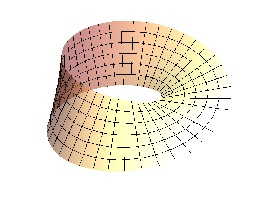
\includegraphics[scale=.75]{Mobius_strip}\\
We start with a surface $S$ that has a tangent plane at every point $(x,y,z)$ on $S$ (except at any boundary point). There are two unit normal vectors $\vec{n}_1$ and $\vec{n}_2 = -\vec{n}_1$ at $(x,y,z)$.\\
If it is possible to choose a unit normal vector $\vec{n}$ at every such point $(x,y,z)$ so that $\vec{n}$ varies continuously over $S$, then $S$ is called an oriented surface and the given choice of $\vec{n}$ provides $S$ with an orientation.
\end{def2}
\begin{def2}
For a surface $z=g(x,y)$ given as the graph of $g$, we have a natural orientation given by the unit vector
$$\vec{n} = \frac{-\frac{\partial g}{\partial x}\vec{i} - \frac{\partial g}{\partial y}\vec{j}+\vec{k}}{\sqrt{1 + \left( \frac{\partial z}{\partial x}\right)^2 + \left( \frac{\partial z}{\partial y}\right)^2}}$$
If $S$ is a smooth orientable surface given in parametric form by a vector function $\vec{r}(u,v)$, then it is automatically supplied with the orientation of the unit normal vector
$$\vec{n} = \frac{\vec{r}_u\times\vec{r}_v}{||\vec{r}_u\times\vec{r}_v||}$$
\end{def2}
\begin{def2}[Flux]
If $\vec{F}$ is a continuous vector field defined on an oriented surface $S$with unit normal vector $\vec{n}$, then the surface integral of $\vec{F}$ over $S$ is
$$\iint_S \vec{F}\cdot d\vec{S} = \iint_S\vec{F}\cdot\frac{\vec{r}_u\times\vec{r}_v}{||\vec{r}_u\times\vec{r}_v||} = \iint_D\left[ \vec{F}(\vec{r}(u,v))\cdot \frac{\vec{r}_u\times\vec{r}_v}{||\vec{r}_u\times\vec{r}_v||}\right]||\vec{r}_u\times\vec{r}_v||dA = \iint_S \vec{F}\cdot \vec{n}dS$$
This integral is also called the flux of $\vec{F}$ across $S$.
\end{def2}
\section{Stokes' Theorem}
Stokes' Theorem\footnote{Stokes' Theorem is names after the Irish mathematical physicist Sir George Stokes (1819-1903). Stokes was a professor at Cambridge University (in fact he held the same position as Newton, Lucasian Professor of Mathematics) and was especially noted for his students of fluid flow and light. What we call Stokes' Theorem was actually discovered by the Scottish physicist Sir William Thomson (1824-1907, known as Lord Kelvin). Stokes learned of this theorem in a letter from Thomson in 1850 and asked students to prove it on an examination at Cambridge University in 1854. We don't know if any of those students was able to do so} can be regarded as a higher-dimensional version of Green's Theorem. Whereas Green's Theorem relates a double integral over a plane region $D$  to a line integral around its boundary curve, Stokes' Theorem relates a surface integral over a surface $S$ to a line integral around the boundary curve of $S$ which is a space curve.
\begin{thm2}[Stokes' Theorem]
Let $S$ be an oriented piece-wise smooth surface that is bounded by a simple, closed, piece-wise smooth boundary curve $C$ with positive orientation. Let $\vec{F}$ be a vector field whose components have continuous partial derivatives on an open region in $\mathbb{R}^3$ that contains $S$. Then
$$\int_C\vec{F}\cdot d\vec{r} = \iint_S\curl\vec{F}\cdot d\vec{S}$$
\end{thm2}
\begin{proof}[Proof of a special case of Stokes' Theorem]
We assume that the equation of $S$ is $z=g(x,y), (x,y)\in D$, where $g$ has continuous second-order partial derivatives and $D$ is a simple plane region whose boundary curve $C_1$ corresponds to $C$. If the orientation of $S$ is upward, then the positive orientation of $C$ coresponds to the positive orientation of $C_1$. We are also given that $\vec{F} = P\vec{i} + Q\vec{j} + R\vec{k}$. where the partial derivatives of $P, Q$, and d$R$ are continuous.\\ Since $S$ is a graph of a function, we can replace $\vec{F}$ with $\curl\vec{F}$. The result is
$$\iint_S\curl\vec{F}\cdot d\vec{S} = \iint_D\left[ -\left( \frac{\partial R}{\partial y} - \frac{\partial Q}{\partial z}\right)\frac{\partial z}{\partial x}-\left( \frac{\partial R}{\partial y} - \frac{\partial Q}{\partial z}\right)\frac{\partial z}{\partial y}+\left( \frac{\partial R}{\partial y} - \frac{\partial Q}{\partial z}\right)\right]dA$$
where the partial derivatives of $P, Q$, and $R$ are evaluated at $(x,y,g(x,y))$. If 
$$x=x(t), y=y(t), a\leq t b\leq$$
is a parametric representation of $C_1$, then a parametric representation of $C$ is 
$$x=x(t), y=y(t), z=g(x(t),y(t)), a\leq t \leq b$$
This allows us, with the aid of the Chain Rule, to evaluate the line integral as follows:
$$\int_C\vec{F}\cdot d\vec{r} = \int_a^b\left( P\frac{dx}{dt} + Q\frac{dy}{dt} + R\frac{dz}{dt}\right)dt = \int_a^b\left[ P\frac{dx}{dt}+Q\frac{dy}{dt} + R\left(\frac{\partial z}{\partial x}\frac{dx}{dt} + \frac{\partial z}{\partial y}\frac{dy}{dt}\right)\right]dt$$
$$=\int_a^b\left[\left(P+R\frac{\partial z}{\partial x}\right)\frac{dx}{dt}+\left(Q + R\frac{\partial z}{\partial y}\right)\frac{dy}{dt}\right]dt$$
$$=\int_{C_1}\left(P+R\frac{\partial z}{\partial x}\right)dx + \left( Q+R\frac{\partial z}{\partial y}\right)dy = \iint_D\left[\frac{\partial}{\partial x}\left( Q+R\frac{\partial z}{\partial y}\right) - \frac{\partial}{\partial y}\left( P+R\frac{\partial z}{\partial x}\right)\right]dA$$
where we have used Green's Theorem in the last step. Then using the Chain Rule again and remembering that $P,Q$, and $R$ are functions of $x,y$, and $z$ and that $S$ is itself a function of $x$ and $y$, we get
$$\int_C\vec{F}\cdot d\vec{r} = \iint_D\left[\left(\frac{\partial Q}{\partial x} + \frac{\partial Q}{\partial z}\frac{\partial z}{\partial x} + \frac{\partial R}{\partial x}\frac{\partial z}{\partial y} +\frac{\partial R}{\partial z}\frac{\partial z}{\partial y}\frac{\partial z}{\partial x} + R\frac{\partial ^2z}{\partial y\partial x}\right)\right] dA$$
Four of the terms in this double integral cancel and the remaining six terms can be arranged to coincide with the right side. Therefore
$$\int_C\vec{F}\cdot d\vec{r} = \iint_S\curl\vec{F}\cdot d\vec{S}$$
\end{proof}
\section{The Divergence Theorem}
Previously we rewrote Green's Theorem in a vector version as
$$\int_C\vec{F}\cdot\vec{n}ds = \iint_D \diverg\vec{F}(x,y)dA$$
where $C$ is the positively oriented boundary curve of the plane region $D$. If we were seeking to extend this theorem to vector fields on $\mathbb{R}^3$, we might make the guess that
$$\iint_S\vec{F}\cdot \vec{n}dS = \iiint_E \diverg\vec{F}(x,y,z)dV$$
where $S$ is the boudary surface of the solid region $E$. 
\begin{thm2}[The Divergence Theorem\footnote{The Divergence Theorem is sometimes called Gauss's Theorem after the great German mathematician Karl Friedrich Gauss (1777-1855), who discovered this theorem during his investigation of electrostatics. In Eastern Europe the Divergence Theorem is known as Ostrogradsky's Theorem after the Russian mathematician Mikhail Ostrogradsky (1801-1862), who published this result in 1826}]
Let $E$ be a simple solid region and let $S$ be the boundary surface of $E$, given with positive, or outward, orientation. Let $\vec{F}$ be a vector field whose component functions have continuous partial derivatives on an open region that contains $E$. Then
$$\iint_S\vec{F}\cdot \vec{n}dS = \iiint_E \diverg\vec{F}(x,y,z)dV$$
\end{thm2}
\begin{proof}
It suffices to prove the theorem for rectangular prisms; the Riemann-sum nature of the triple integral then guarantees the theorem for arbitrary regions.
Let: $R=\{(x,y,z)|a_1\leq x\leq a_2,b_1\leq y\leq b_2,c_1\leq z\leq c_2\}$ and let $S=\partial R$, oriented outward.\\
Then : $S=A_1\cup A_2\cup A_3\cup A_4\cup A_5\cup A_6$ where $A_1,A_2$ are those sides perpendicular to the $x$-axis, $A_3,A_4$ perpendicular to the $y$ axis, and $A_5,A_6$ are those sides perpendicular to the $z$-axis, and in all cases the lower subscript indicates a side closer to the origin.\\
Let: $F=M\vec{i}+N\vec{j}+P\vec{k}$ where $M,N,P:\mathbb{R}^3\to\mathbb{R}$. Then:
$$\iiint_R\grad\cdot\vec{F}dV = \iiint_R\left( \frac{\partial M}{\partial x} +  \frac{\partial N}{\partial y} +  \frac{\partial P}{\partial z}\right)dxdydz$$
$$\iiint_R\frac{\partial M}{\partial x}dxdydz + \iiint_M\frac{\partial N}{\partial y}dxdydz + \iiint_M\frac{\partial P}{\partial z}dxdydz$$
$$\int_{c_1}^{c_2}\int_{b_1}^{b_2} (M(a_2,y,z)-M(a_1,y,z))dydz + \int_{c_1}^{c_2}\int_{a_1}^{a_2} (N(x,b_2,z)-M(x,b_1,z))dxdz + \int_{b_1}^{b_2}\int_{a_1}^{a_2} (P(x,y,c_2)-P(x,y,c_1))dxdy$$    
Thus:
$$\iiint_R\grad\cdot\vec{F}dV = \iint_{A_2}Mdydz-\iint_{A_2}Mdydz + \iint_{A_4}Ndxdz-\iint_{A_3}Ndxdz + \iint_{A_6}Pdxdy-\iint_{A_5}Pdxdy$$
and so:
$$\iiint_R\grad\cdot\vec{F} = \iint_{\partial R}\vec{F}\cdot\vec{n}dS$$
\end{proof}

\part{Linear Algebra}
\chapter{Linear Equations}
\section{Matrices, Vectors, and Gauss-Jordan Elimination}
A matrix with only one column is called a vector, or simply a vector. The entries of a vector are called its components. The set of all column vectors with \textit{n} components is denoted by $\mathbb{R}^n$; we will refer to $\mathbb{R}^n$ as a \textit{vector space}.\\
A matrix with only one row is called a row vector.\\
The standard representation of a vector 
$$\vec{v}=\left[_y^x\right]$$
in the Cartesian coordinate plane is as an \textit{arrow} (a directed line segment) from the origin to the point $(x,y)$.

The standard representation of a vector in $\mathbb{R}^3$ is defined analogously.
\paragraph{Solving a system of linear equations-}
We proceed from equation to equation, from top to bottom.

Suppose we get to the $i$th equation. Let $x_j$ be the leading variable of the system consisting of the $i$th and all the subsequent equations. (If no variables are left in this system, then the process comes to an end.)
\begin{itemize}
\item[1.] If $x_j$ does not appear in the $i$th equation, swap the $i$th equation with the first equation below that does contain $x_j$.
\item[2.] Suppose the coefficient of $x_j$ in the $i$th equation is $c$; thus this equation is of the form $cx_j + \cdots = \cdots$. Divide the $i$th equation by $c$.
\item[3.] Eliminate $x_j$ from all other equations, above and below the $i$th, by subtracting suitable multiples of the $i$th equation from the others
\end{itemize}
Now proceed to the next equation.

If an equation \textit{zero} = \textit{nonzero} emerges in this process, then the system fails to have solutions; the system is \textit{inconsistent}.

When you are through without encountering an inconsistency, solve each equation for its leading variable. You may choose the non leading variables freely; the leading variables are then determined by these choices.
\section{Solutions of Linear Systems: Matrix Algebra}
\begin{thm2}[Number of Solutions of a Linear System]
A system of equations is said to be \textit{consistent} if there is at least one solution; it is \textit{inconsistent} if there are no solutions.

A linear system is inconsistent if and only if the reduced row echelon form of its augmented matrix contains the row $[0,  0,  \cdots, 0 | 1 ]$, representing the equation $0=1$.

If a linear system is consistent, then it has either
\begin{itemize}
\item[1.] \textit{Infinitely many solutions} (if there is at least one free variable), or
\item[2.] \textit{exactly one solution} (if all the variables are leading)
\end{itemize}
\end{thm2}
\begin{def2}[The Rank of a Matrix]
The rank of a matrix $A$ is the number of leading $1$'s in $\rref(A)$.
This is for the coefficient matrix only. We do not count pivots in the augmented part of matrices.

Consider a system of $n$ linear equations in $m$ variables; its coefficient matrix $A$ has the size $n\times m$.
\begin{itemize}
\item[1.] The inequalities rank$(A)\leq n$ and rank$(A)\leq m$ hold.
\item[2.] If rank$(A)=n$, then the system is consistent.
\item[3.] If rank$(A)=m$, then the system has at most one solution.
\item[4.] If rank$(A)< m$, then the system has either infinitely many solutions or none.
\end{itemize}
\end{def2}
\begin{thm2}[Systems with Fewer Equations than Variables]
A linear system with fewer equations than unknowns has either no solutions or infinitely many solutions.

To put it differently, if a linear system has a unique solution, then there must be at least as many equations as there are unknowns
\begin{proof}
Consider a linear system of $n$ equations in $n$ variables. 

If rank($A)<n$, then there will be free variables $(n - $rank $A$ of them), so that the system has either no solutions or infinitely many solutions.

If rank($A)=n$, then there are no free variables, so that there cannot be infinitely many solutions. Furthermore, there must be a leading 1 in every row of $\rref(A)$, so that the system is consistent. We conclude that the system must have a unique solution in this case.
\end{proof}
\end{thm2}
\begin{thm2}[Systems of $n$ Equations in $n$ Variables]
A linear system of $n$ equations in $n$ variables has a unique solution if and only if the rank of its coefficient matrix $A$ is $n$. In this case,
$$\rref(A)=\left[\begin{array}{c c c c c}
1 & 0 & 0 & \cdots & 0\\
0 & 1 & 0 & \cdots & 0\\
0 & 0 & 1 & \cdots & 0\\
\vdots & \vdots & \vdots & \ddots & \vdots\\
0 & 0 & 0 & \cdots & 1\\

\end{array}\right]$$
the $n\times n$ matrix with 1's along the diagonal and 0's everywhere else.
\end{thm2}
\begin{def2}[Sums of Matrices]
The sum of two matrices of the same size is defined entry by entry.
$$\left[\begin{array}{c c c}
a_{11} & \cdots & a_{1m}\\
\vdots & & \vdots\\
a_{n1} & \cdots & a_{nm}
\end{array}\right]+ \left[\begin{array}{c c c}
b_{11} & \cdots & b_{1m}\\
\vdots & & \vdots\\
b_{n1} & \cdots & b_{nm}
\end{array}\right] = \left[\begin{array}{c c c}
a_{11}+b_{11} & \cdots & a_{1m} + b_{1m}\\
\vdots & & \vdots\\
a_{n1} + b_{n1} & \cdots & a_{nm} + b_{nm}
\end{array}\right]$$
The product of a scalar with a matrix is defined entry by entry:
$$k\left[\begin{array}{c c c}
a_{11} & \cdots & a_{1m}\\
\vdots & & \vdots\\
a_{n1} & \cdots & a_{nm}
\end{array}\right]= \left[\begin{array}{c c c}
ka_{11} & \cdots & ka_{1m}\\
\vdots & & \vdots\\
ka_{n1} & \cdots & ka_{nm}
\end{array}\right]$$
\end{def2}
\begin{def2}[Dot Product of Vectors]
Consider two vectors $\vec{v}$ and $\vec{w}$ with components $v_1 \cdots v_n$ and $w_1 \cdots w_n$, respectively. Here $\vec{v}$ and $\vec{w}$ may be column or row vectors, and they need not be of the same type. The dot product of $\vec{v}$ and $\vec{w}$ is defined to be the scalar
$$\vec{v} \cdot \vec{w} = v_1w_1 + \cdots + v_nw_n$$
\end{def2}
\begin{def2}[The Product of $\vec{x}$]
If $A$ is an $n\times m$ matrix with row vectors $\vec{w_1}, \cdots , \vec{w_m}$, and $\vec{x}$ is a vector $\mathbb{R}^m$, then
$$A\vec{x}=\left[ \begin{array}{c c c}
- & \vec{w_1} & -\\
& \vdots & \\
- & \vec{w_n} & -
\end{array}\right] \vec{x} = \left[ \begin{array}{c}
\vec{w}_1 \cdot \vec{x}\\
\vdots\\
\vec{w}_n \cdot \vec{x}
\end{array}\right]$$
In words, the $i$th component of $A\vec{x}$ is a column vector with $n$ components, that is, a vector in $\mathbb{R}^n$
\end{def2}
\begin{thm2}[The Product $A\vec{x}$ in terms of the columns of $A$]
If the column vectors of an $n\times m$ matrix $A$ are $\vec{v}_1, \cdots , \vec{v}_m$
and $\vec{x}$ is a vector in $\mathbb{R}^n$ with components $x_1, \cdots , x_m$, then
$$A\vec{x}=\left[ \begin{array}{c c c}
| & & |\\
\vec{v}_1 & & \vec{v}_m\\
| & & |
\end{array}\right]\left[ \begin{array}{c}
x_1\\
\vdots\\
x_m
\end{array}\right] = x_1 \vec{v}_1 + \cdots + x_m \vec{v}_m$$
\begin{proof}
As usual, we denote the rows of $A$ by $\vec{w}_1, \cdots , \vec{w}_m$ and the entries by $a_{ij}$. It suffices to show that the $i$th component of $A\vec{x}$ is equal to the $i$th component of $x_1\vec{v}_1 + \cdots + x_m\vec{v}_m$, for $i=1,...,n$. Now
$$(i\text{th component of }A\vec{x})\underbrace{=}_{Step 1} \vec{w_i}\cdot \vec{x} = a_{i1}x_1 + \cdots a_{im}x_m$$
$$= x_1(i\text{th component of} \vec{v}_1) + \cdots + x_m (i\text{th component of } \vec{v}_m)$$
$$\underbrace{=}_{Step 4} i\text{th component of } x_1 \vec{v}_1 + \cdots + x_m \vec{v}_m$$
\end{proof}
\end{thm2}
\begin{def2}[Linear Combinations]
A vector $\vec{b}$ in $\mathbb{R}^n$ is called a linear combination of the vectors $\vec{v}_1,...,\vec{v}_m$ in $\mathbb{R}^n$ if there exists scalars $x_1, ..., x_m$ such that
$$\vec{b} = x_1 \vec{v}_1 + \cdots + x_m \vec{v}_m$$
\end{def2}
\begin{thm2}[Algebraic Rules for $A\vec{x}$]
If $A$ is an $n\times m$ matrix; $\vec{x}$ and $\vec{y}$ are vectors in $\mathbb{R}^m$; and $k$ is a scalar, then
\begin{itemize}
\item[1.] $A(\vec{x} + \vec{y}) = A\vec{x} + A\vec{y}$, and
\item[2.] $A(k\vec{x}) = k(A\vec{x})$
\end{itemize}
\end{thm2}
\begin{thm2}[Matrix Form of a Linear System]
We can write the linear system with augmented matrix $[A|\vec{b}]$ in matrix for as
$$A\vec{x} = \vec{b}$$
\end{thm2}

\chapter{Linear Transformations}
\section{Introduction to Linear Transformations}
\begin{def2}[Linear Transformations]
A function $T:\mathbb{R}^m\to \mathbb{R}^n$ is called a linear transformation if there exists an $n\times m$ matrix $A$ such that
$$T(\vec{x}) = A(\vec{x})$$
for all $\vec{x}$ in the vector space $\mathbb{R}^n$
\end{def2}
\begin{thm2}[The Columns of the Matrix of a Linear Transformation]
Consider a linear transformation $T: \mathbb{R}^m \to\mathbb{R}^n$. Then, the matrix of $T$ is
$$A=\left[\begin{array}{c c c c}
| & | & & |\\
T(\vec{e}_1) & T(\vec{e}_2) & \cdots & T(\vec{e}_m)\\
| & | & & |
\end{array}\right], \text{where } \vec{e}_1 = \left[ \begin{array}{c}
0\\
0\\
\vdots \\
1\\
\vdots \\
0
\end{array}\right] \leftarrow i\text{th}$$
\end{thm2}
\begin{thm2}[Linear Transformations]
A transformation $T:\mathbb{R}^m \to \mathbb{R}^n$ is linear if and only if
\begin{itemize}
\item[1.] $T(\vec{v} + \vec{w}) = T(\vec{v}) + T(\vec{w})$, for all vectors $\vec{v}$ and $\vec{w}$ in $\mathbb{R}^m$, and
\item[2.] $T(k\vec{v}) = kT(\vec{v})$, for all vectors $\vec{v}$ in $\mathbb{R}^m$ and scalars $k$.
\end{itemize}
\begin{proof}
To prove the converse, consider a transformation $T:\mathbb{R}^n \to \mathbb{R}^m$ that satisfies equations (1.) and (2.). We must show that there exists a matrix $A$ such that $T(\vec{x}) = A\vec{x}\forall \vec{x}\in \mathbb{R}^m$. Let $\vec{e}_1\cdots , \vec{e}_m$ be the standard vectors.
$$T(\vec{x}) = T\left[ \begin{array}{c}
x_1\\
x_2\\
\vdots \\
x_m
\end{array}\right] = T(x_1 \vec{e}_1) + x_2 \vec{e}_2 + \cdots + x_m \vec{e}_m)$$
$$=T(x_1 \vec{e}_1) + T(x_2 \vec{e}_2) + \cdots + T(x_m \vec{e}_m)$$
$$=x_1T(\vec{e}_1) + x_2T (\vec{e}_2) + \cdots + x_m T(\vec{e}_m)$$
$$=\left[ \begin{array}{c c c c}
| & | & & |\\
T(\vec{e}_1) & T(\vec{e}_2) & \cdots & T(\vec{e}_m)\\
| & | & & |
\end{array}\right]\left[ \begin{array}{c}
x_1\\
x_2\\
\vdots \\
x_m
\end{array}\right] = A \vec{x}$$
\end{proof}
\end{thm2}
\section{Linear Transformations in Geometry}
\begin{def2}[Orthogonal Projections]
Consider a line $L$ in the coordinate plane, running through the origin. Any vector $\vec{x}$ in $\mathbb{R}^2$ can be written uniquely as
$$\vec{x} = \vec{x}^{\parallel} + \vec{x}^{\perp}$$
where $\vec{x}^{\parallel}$ is parallel to the line $L$, and $\vec{x}^{\perp}$ is perpendicular to $L$.

The transformation $T(\vec{x})= \vec{x}^{\parallel}$ from $\mathbb{R}^2$ to $\mathbb{R}^2$ is called the orthogonal projection of $\vec{x}$ onto $L$, often denoted by $\text{proj}_L( \vec{x})$. If $\vec{w}$ is a nonzero vector parallel to $L$, then
$$\text{proj}_L( \vec{x}) = \left(\frac{\vec{x} \cdot \vec{w}}{\vec{w} \cdot \vec{w}}\right) \vec{w}$$
In particular, if $\vec{u}$ = $\left[ \begin{array}{c}
u_1\\
u_2
\end{array}\right]$ is a unit vector parallel to $L$, then
$$\text{proj}_L( \vec{x}) = (\vec{x} \cdot \vec{u}) \vec{u}$$
The transformation $T (\vec{x}) = \text{proj}_L (\vec{x})$ is linear, with matrix
$$\frac{1}{w_1^2 + w_2^2}\left[ \begin{array}{c c}
w_1^2 & w_1w_2\\
w_1w_2 & w_2^2
\end{array}\right] = \left[ \begin{array}{c c}
u_1^2 & u_1u_2\\
u_1u_2 & u_2^2
\end{array}\right]$$
\end{def2}
\begin{def2}[Reflections]
Consider a line $L$ in the coordinate plane, running through the origin, and let $\vec{x} = \vec{x}^{\parallel} + \vec{x}^{\perp}$ be a vector in $\mathbb{R}^n$. The linear transformation $T(\vec{x}) = \vec{x}^{\parallel} - \vec{x}^{\perp}$ is called the reflection of $\vec{x}$ about $L$, often denoted by $\text{ref}_L( \vec{x}):$
$$\text{ref}_L(\vec{x}) = \vec{x}^{\parallel} - \vec{x}^{\perp}$$
We have a formula relating $\text{ref}_L(\vec{x})$ to $\text{proj}_L(\vec{x})$:
$$\text{ref}_L(\vec{x}) = 2\text{proj}_L(\vec{x}) - \vec{x}=2( \vec{x} \cdot \vec{u}) \vec{u} - \vec{x}$$
The matrix of $T$ is of the form $\left[ \begin{array}{c c}
a & b\\
b & -a
\end{array}\right]$, where $a^2 + b^2 = 1$. Conversely, any matrix of this form represents a reflection about a line.
\end{def2}
\begin{thm2}[Rotations]
The matrix of a counterclockwise rotation in $\mathbb{R}^2$ through an angle $\theta$ is
$$\left[ \begin{array}{c c}
\cos\theta & -\sin\theta\\
\sin\theta & \cos\theta
\end{array}\right]$$
\begin{itemize}
\item[Note:] This matrix is of the form $\left[ \begin{array}{c c}
a & -b\\
b & a
\end{array}\right]$, where $a^2 + b^2 = 1$. Conversely, any matrix of this form represents a rotation.
\end{itemize}
\end{thm2}
\begin{thm2}[Rotations Combined with Scaling]
A matrix of the form $\left[ \begin{array}{c c}
a & -b\\
b & a
\end{array}\right]$ represents a rotation combined with a scaling.

More precisely, if $r$ and $\theta$ are the polar coordinates of vector $\left[ \begin{array}{c}
a\\
b
\end{array}\right]$, then $\left[ \begin{array}{c c}
a & -b\\
b & a
\end{array}\right]$ represents a rotation through $\theta$ combined with a scaling by $r$
\end{thm2}
\begin{thm2}[Horizontal and Vertical Shears]
The matrix of a horizontal shear is of the form $\left[ \begin{array}{c c}
1 & k\\
0 & 1
\end{array}\right]$, and the matrix of a vertical shear is of the form $\left[ \begin{array}{c c}
1 & 0\\
k & 1
\end{array}\right]$, where $k$ is an arbitrary constant.
\end{thm2}
\section{Matrix Products}
\begin{def2}[Matrix Multiplication]
Although this definition of matrix multiplication does not give us concrete instructions for computing the product of two numerically given matrices, such instructions can be derived easily from the definition.
\begin{itemize}
\item[1.] Let $B$ be an $n\times p$ matrix and $A$ a $q\times m$ matrix. The product $BA$ is defined if and only if $p=q$.
\item[2.] If $B$ is an $n\times p$ matrix and $A$ a $p\times m$ matrix, then the product $BA$ is defined as the matrix of the linear transformation $T(\vec{x}) = B(A(\vec{x}))$. This means that $T(\vec{x}) = B(A(\vec{x})) = (BA) \vec{x}$, for all $\vec{x}$ in the vector space $\mathbb{R}^m$. The product $BA$ is an $n\times m$ matrix.
\end{itemize}
\end{def2}
\begin{thm2}[The Columns of the Matrix Product]
Let $B$ be an $n\times p$ matrix and $A$ a $p\times m$ matrix with columns $\vec{v}_1, \vec{v}_2, \cdots, \vec{v}_m$. Then the product $BA$ is
$$BA=B\left[ \begin{array}{c c c c}
| & | & & |\\
\vec{v}_1 & \vec{v}_2 & \cdots & \vec{v}_m\\
| & | & & |
\end{array}\right] = \left[ \begin{array}{c c c c}
| & | & & |\\
B\vec{v}_1 & B\vec{v}_2 & \cdots & B\vec{v}_m\\
| & | & & |
\end{array}\right]$$
To find $BA$, we can multiply $B$ with the columns of $A$ and combine the resulting vectors.
\end{thm2}
\begin{thm2}[Matrix Multiplication is Noncommutative]
$AB\neq BA$, in general. However, at times it does happen that $AB=BA$; then we say that the matrices $A$ and $B$ commute.
\end{thm2}
\begin{thm2}[The Entries of the Matrix Product]
Let $B$ be an $n\times p$ matrix and $A$ a $p\times m$ matrix. The $ij$th entry of $BA$ is the dot product of the $i$th row of $B$ with the $j$th column of $A$.
$$BA = \left[ \begin{array}{c c c c}
b_{11} & b_{12} & \cdots & b_{1p}\\
b_{21} & b_{22} & \cdots & b_{2p}\\
\vdots & \vdots & \ddots & \vdots\\
b_{i1} & b_{i2} & \cdots & b_{ip}\\
\vdots & \vdots & \ddots & \vdots\\
b_{n1} & b_{n2} & \cdots & b_{np}
\end{array}\right]\left[ \begin{array}{c c c c c c}
a_{11} & a_{12} & \cdots & a_{1j} & \cdots & a_{1m}\\
a_{21} & a_{22} & \cdots & a_{2j} & \cdots & a_{2m}\\
\vdots & \vdots & \ddots & \vdots & \ddots & \vdots\\
a_{p1} & a_{p2} & \cdots & b_{pj} & \cdots & a_{pm}
\end{array}\right]$$
is the $n\times m$ matrix whose $ij$th entry is
$$b_{i1}a_{1j} + b_{i2}a_{2j} + \cdots + b_{ip}a_{pj} = \Sigma_{k=1}^p b_{ik}a_{kj}$$
\end{thm2}
\begin{thm2}[Multiplying with the Identity Matrix]
For an $n\times m$ matrix $A$,
$$AI_m = I_nA = A$$
\end{thm2}
\begin{thm2}[Matrix Multiplication is Associative]
$$(AB)C = A(BC)$$
We can simply write $ABC$ for the product $(AB)C = A(BC)$.
\end{thm2}
\begin{thm2}[Distributive Property of Matrices]
If $A$ and $B$ are $n\times p$ matrices, and $C$ and $D$ are $p\times m$ matrices, then 
$$A(C+D) = AC + AD, \text{ and}$$
$$(A+B)C = AC + BC$$
\end{thm2}
\begin{thm2}
If $A$ is an $n\times p$ matrix, $B$ is a $p\times m$ matrix, and $k$ is a scalar, then
$$(kA)B = A(kb) = k(AB)$$
\end{thm2}
\begin{thm2}[Multiplying Block Matrices]
Block matrices can be multiplied as though the blocks were scalars:
$$AB = \left[ \begin{array}{c c c c}
A_{11} & A_{12} & \cdots & A_{1p}\\
A_{21} & A_{22} & \cdots & A_{2p}\\
\vdots & \vdots & \ddots & \vdots\\
A_{i1} & A_{i2} & \cdots & A_{ip}\\
\vdots & \vdots & \ddots & \vdots\\
A_{n1} & A_{n2} & \cdots & A_{np}
\end{array}\right]\left[ \begin{array}{c c c c c c}
B_{11} & B_{12} & \cdots & B_{1j} & \cdots & B_{1m}\\
B_{21} & B_{22} & \cdots & B_{2j} & \cdots & B_{2m}\\
\vdots & \vdots & \ddots & \vdots & \ddots & \vdots\\
B_{p1} & B_{p2} & \cdots & B_{pj} & \cdots & B_{pm}
\end{array}\right]$$
is the block matrix whose $ij$th block is the matrix
$$A_{i1}B_{1j} + A_{i2}B_{2j} + \cdots + A_{ip}B_{pj} = \Sigma_{k=1}^p A_{ik}B_{kj}$$
provided that all the products $A_{ik}B_{kj}$are defined.
\end{thm2}
\section{The Inverse of a Linear Transformation}
\begin{def2}[Invertible Functions]
A function $T:X\to Y$ is called invertible if the equation $T(x)=y$ has a unique solution $x\in X, \forall y\in Y$.

In this case, the inverse $T^{-1}:Y\to X$ is defined by
$$T^{-1}(y) = \text{(the unique }x\in X \ni T(x) = y$$

Consider the case of a linear transformation $T:\mathbb{R}^n\to \mathbb{R}^n$ given by
$$\vec{y} = T(\vec{x}) = A\vec{x}$$
where $A$ is an $n\times n$ matrix. According to our definition, the linear transformation $\vec{y} = T(\vec{x}) = A\vec{x}$ is invertible if the linear system $A\vec{x} = \vec{y}$ has a unique solution $\vec{x}\in \mathbb{R}^n \forall \vec{y}\in \mathbb{R}^n$. By a previous theorem, this is the case if and only if rank($A)=n$, or equivalently, if
$$\rref(A) = \left[ \begin{array}{c c c c c}
1 & 0 & 0 & \cdots & 0\\
0 & 1 & 0 & \cdots & 0\\
0 & 0 & 1 & \cdots & 0\\
\vdots & \vdots & \vdots & \ddots & \vdots\\
0 & 0 & 0 & \cdots & 1\\
\end{array}\right] = I_n$$
\end{def2}
\begin{def2}[Invertible Matrices]
A square matrix $A$ is said to be invertible if the linear transformation $\vec{y} = T(\vec{x}) = \vec{x}$ is invertible. In this case, the matrix of $T^{-1}$ is denoted by $A^{-1}$. If the linear transformation $\vec{y} = T(\vec{x}) = A\vec{x}$ is invertible, then its inverse is $\vec{x} = T^{-1}(\vec{y}) = A^{-1}\vec{y}$
\end{def2}
\begin{thm2}[Invertibility]
An $n\times n$ matrix $A$ is invertible $\iff \rref(A)=I_n\text{ or, equivalently rank}(A) = n$ 
\end{thm2}
\begin{thm2}[Invertibility and Linear Systems]
Let $A$ be an $n\times n$ matrix.
\begin{itemize}
\item[a.] Consider a vector $\vec{b}\in \mathbb{R}^n$. If $A$ is invertible, then the system $A\vec{x}=\vec{b}$ has the unique solution $\vec{x}=A^{-1}\vec{b}$. If $A$ is noninvertible, then the system $A\vec{x}=\vec{b}$ has infinitely many solutions of none.
\item[b.] Consider the special case when $\vec{b}=\vec{0}$. The system $A\vec{x}=\vec{0}$ has $\vec{x}=\vec{0}$ as a solution. If $A$ is invertible, then this is the only solution. If $A$ is noninvertible, then the system $A\vec{x}=\vec{0}$ has infinitely many solutions.
\end{itemize}
\end{thm2}
\begin{thm2}[Finding the Inverse of a Matrix]
To find the inverse of an $n\times n$ matrix $A$, form the $n\times (2n)$ matrix $[A|I_n]$ and compute $\rref[A|I_n]$.
\begin{itemize}
\item If $\rref[A|I_n]$ is of the form $[I_n|B]$, then $A$ is invertible, and $A^{-1}=B$
\item If $\rref[A|I_n]$ is of another form (i.e., its left half fails to be $I_n$), then $A$ is not invertible. Note that the left half of $\rref[A|I_n]$ is $\rref(A)$.
\end{itemize}
\end{thm2}
\begin{thm2}[Multiplying with the Inverse]
For an invertible $n\times n$ matrix $A$, 
$$A^{-1}A = I_n \text{  and  } AA^{-1} = I_n$$
\end{thm2}
\begin{thm2}[The Inverse of a Product of Matrices]
If $A$ and $B$ are invertible $n\times n$ matrices, then $BA$ is invertible as well, and
$$(BA)^{-1} = A^{-1}B^{-1}$$
\end{thm2}
\begin{thm2}[A Criterion for Invertibility]
Let $A$ and $B$ be two $n\times n$ matrices such that
$$BA=I_n$$
Then
\begin{itemize}
\item[a.] $A$ and $B$ are both invertible
\item[b.] $A^{-1}=B$ and $B^{-1}=A$, and
\item[c.] $AB=I_n$
\end{itemize}
\begin{proof}
To demonstrate that $A$ is invertible, it suffices to show that the linear system $A\vec{x}=\vec{0}$ has only the solution $\vec{x}=\vec{0}$. If we multiply the equation $A\vec{x}=\vec{0}$ by $B$ from the left, we find that $BA\vec{x}=B\vec{0}=\vec{0}$. It follows that $\vec{x}=I_n\vec{x} =BA\vec{x}=\vec{0}$, as claimed. Therefore, $A$ is invertible. If we multiply the equation $BA=I_n$ by $A^{-1}$ from the right, we find that $B=A^{-1}$. Matrix $B$, being the inverse of $A$, is itself invertible, and $B^{-1}=(A^{-1})^{-1}=A$. Finally, $AB=AA^{-1}=I_n$
\end{proof}
\end{thm2}
\begin{thm2}[Inverse and Determinant of a $2\times 2$ Matrix]
\begin{itemize}
\item[a.] The $2\times 2$ 
$$A=\left[\begin{array}{c c}
a & b\\
c & d
\end{array}\right]$$
is invertible if and only if $ad-bc\neq 0$
Quantity $ad-bc$ is called the determinant of $A$, written $\det(A)$:
$$\det(A) = \det \left[ \begin{array}{c c}
a & b\\
c & d
\end{array}\right]=ad-bc$$
\item[b.] If
$$A = \left[ \begin{array}{c c}
a & b\\
c & d
\end{array}\right]$$
is invertible, then
$$\left[ \begin{array}{c c}
a & b\\
c & d
\end{array}\right]^{-1}=\frac{1}{ad-bc}\left[ \begin{array}{c c}
d & -b\\
-c & a
\end{array}\right]= \frac{1}{\det(A)}
\left[ \begin{array}{c c}
d & -b\\
-c & a
\end{array}\right]$$
\end{itemize}
\end{thm2}
\begin{thm2}[Geometrical Interpretation of the Determinant of a $2\times 2$ Matrix]
If $A=[\begin{array}{c c}
\vec{v} & \vec{w}
\end{array}]$ is a  $2\times 2$ matrix with nonzero columns $\vec{v}$ and $\vec{w}$, then
$$\det A = \det [\begin{array}{c c}
\vec{v} & \vec{w}
\end{array}] = ||\vec{v}||\sin \theta||$$
where $\theta$ is the oriented angle from $\vec{v}$ to $\vec{w}$, with $-\pi<\theta \leq \pi$. It follows that
\begin{itemize}
\item $|\det A|=||\vec{v}|| |\sin \theta| ||\vec{w}||$ is the area of the parallelogram spanned by $\vec{v}$ and $\vec{w}$
\item $\det A=0$ if $\vec{v}$ and $\vec{w}$ are parallel, meaning that $\theta=0$ or $\theta = \pi$
\item $\det A >0$ if $0<\theta <\pi$, and
\item $\det A <0$ if $-\pi<\theta <0$
\end{itemize}
\end{thm2}
\chapter{Vectors}
Here we will provide a concise summary of basic facts on vectors\footnote{Josiah Willard Gibbs (1839-1903), a professor of mathematical physics at Yale College, published the first book on vectors, \textit{Vector Analysis}, in 1881. More complicated objects, called quaternions, had earlier been invented by Hamilton as mathematical tools for describing space, but they weren't easy for scientists to use. Quaternions have a scalar part and a vector part. Gibb's idea was to use the vector part separately. Maxwell and Heaviside had similar ideas, but Gibb's approach has proved to be the most convenient way to study space.}. Vectors are defined as matrices with only one column:
$$\vec{v}=\left[ \begin{array}{c}
v_1\\
v_2\\
\vdots\\
v_n
\end{array}\right]$$
The scalars $v_i$ are called the components of the vector. The set of all vectors with $n$ components is denoted by $\mathbb{R}^n$
\section{Vector Algebra}
\begin{def2}[Vector Addition and Scalar Multiplication]
\begin{itemize}
\item[a.] The sum of two vectors $\vec{v}$ and $\vec{w}\in\mathbb{R}^n$ is defined "component wise":
$$\vec{v} + \vec{w}=\left[ \begin{array}{c}
v_1\\
v_2\\
\vdots\\
v_n
\end{array}\right]+\left[ \begin{array}{c}
w_1\\
w_2\\
\vdots\\
w_n
\end{array}\right]=\left[ \begin{array}{c}
v_1+w_1\\
v_2+w_2\\
\vdots\\
v_n+w_n
\end{array}\right]$$
\item[b.] Scalar multiplication is the product of a scalar $k$ and a vector $\vec{v}$ and is defined component wise as well:
$$k\vec{v}=k\left[ \begin{array}{c}
v_1\\
v_2\\
\vdots\\
v_n
\end{array}\right]+\left[ \begin{array}{c}
kv_1\\
kv_2\\
\vdots\\
kv_n
\end{array}\right]$$
\end{itemize}
The negative or opposite of a vector $\vec{v}\in\mathbb{R}^n$ is defined as
$$-\vec{v}=(-1)\vec{v}$$
The difference $\vec{v}-\vec{w}$ of two vectors $\vec{v},\vec{w}\in\mathbb{R}^n$ is defined component wise. Alternatively, we can express the difference of two vectors as
$$\vec{v}-\vec{w}=\vec{v}+(-\vec{w})$$
The vector in $\mathbb{R}^n$ that consists of $n$ zeros is called the zero vector in $\mathbb{R}^n$
$$\vec{0}=\left[ \begin{array}{c}
0\\
0\\
\vdots\\
0
\end{array}\right]$$ 
\end{def2}
\begin{thm2}[Rules of Vector Algebra]
The following formulas will hold for all vectors $\vec{u}, \vec{v}, \vec{w}\in\mathbb{R}^n$ and for all scalars $c$ and $k$:
\begin{itemize}
\item[1.] $(\vec{u}+\vec{v})+\vec{w}= \vec{u}+(\vec{v}+\vec{w})$: Addition is associative.
\item[2.]$\vec{v}+\vec{w}=\vec{w}+\vec{v}$: Addition is commutative
\item[3.] $\vec{v}+\vec{0}=\vec{v}$
\item[4.] $\forall \vec{v}\in \mathbb{R}^n \ni \vec{v}+\vec{x} =\vec{0}$, namely, $\vec{x}=-\vec{v}$
\item[5.] $k(\vec{v}+\vec{w}) =k\vec{v}+k\vec{w}$
\item[6.] $(c+k)\vec{v} = c\vec{v}+ k\vec{v}$
\item[7.] $c(k\vec{v}) = (ck)\vec{v}$
\item[8.] $1\vec{v}=\vec{v}$
\end{itemize}
\end{thm2}
\section{***Geometrical Representation of Vectors***}
\begin{def2}
We say that two vectors are parallel if one of them is a scalar multiple of the other
\end{def2}
\section{Dot Product, Length, Orthogonality}
\begin{def2}
Consider two vectors $\vec{v}$ and $\vec{w}$ with components $v_1, v_2, ..., v_n$ and $w_1, w_2, ... w_n$, respectively. Here $\vec{v}$ and $\vec{w}$ may be column or row vectors, and they need not be of the same type (these conventions are convenient in linear algebra). The dot product of $\vec{v}$ and $\vec{w}$ is defined as
$$\vec{v}\cdot\vec{w}=v_1w_1+v_2w_2+ \cdots + v_nw_n$$
We can interpret the dot product geometrically: If $\vec{v}$ and $\vec{w}$ are two nonzero vectors in $\mathbb{R}^n$, then
$$\vec{v}\cdot\vec{w}=||\vec{v}|| \cos\theta ||\vec{w}||$$
where $\theta$ is the angle enclosed by vectors $\vec{v}$ and $\vec{w}$
\begin{itemize}
\item[Note:] The dot product of two vectors is a scalar
\end{itemize}
\end{def2}
\begin{thm2}[Rules for Dot Products]
The following equations hold for all column or row vectors $\vec{u}, \vec{v}, \vec{w}$ with $n$ components, and for all scalars $k$:
\begin{itemize}
\item[1.] $\vec{v}\cdot\vec{w} = \vec{w}\cdot\vec{v}$
\item[2.] $(\vec{u}+\vec{v})\cdot \vec{w} = \vec{u} \cdot \vec{w} + \vec{v} \cdot \vec{w}$
\item[3.] $(k\vec{v})\cdot \vec{w} = k( \vec{v}\cdot \vec{w})$
\item[4.] $\vec{v}\cdot \vec{v} > 0, \forall \vec{v}\neq \vec{0}$
\end{itemize}
\end{thm2}
\begin{def2}
The length (or norm) $||\vec{x}||$ of a vector $\vec{x}\in \mathbb{R}^n$ is
$$||\vec{x}||=\sqrt{\vec{x} \cdot \vec{x}} = \sqrt{x_1^2 + x_2^2 + \cdots + x_n^2}$$
\end{def2}
\begin{def2}
A vector $\vec{u}\in\mathbb{R}^n$ is called a unit vector if $||\vec{u}||=1$; that is, the length of the vector $\vec{u}$ is 1
\end{def2}
\begin{def2}
Two vectors $\vec{v}$ and $\vec{w}\in \mathbb{R}^n$ are called perpendicular (or orthogonal) if $\vec{v} \cdot \vec{w} = 0$
\end{def2}
\begin{thm2}
If $\theta$ is the angle between the vectors $\vec{a}$ and $\vec{b}$, then
$$\vec{a}\cdot\vec{b}=||\vec{a}||||\vec{b}||\cos \theta$$
\end{thm2}
\begin{proof}
If we apply the Law of Cosines to triangle $OAB$ we get
$$||AB||^2 = ||OA||^2 + ||OB||^2 - 2||OA||||OB||\cos \theta$$
(Observe that the Law of Cosines still applies in the limiting cases when $\theta=0$ or $\pi$, or $\vec{a}=\vec{0}$ or $\vec{b}=\vec{0}$.) But $||OA||=||\vec{a}||$, $||OB|| = ||\vec{b}||$, and $||AB|| = ||\vec{a}-\vec{b}||$, and we get
$$||\vec{a}-\vec{b}||^2 = ||\vec{a}||^2 + ||\vec{b}||^2-2||\vec{a}||||\vec{b}||\cos \theta$$
Using properties of the dot product, we can rewrite the left side of this equation as follows:
$$||\vec{a}-\vec{b}||^2 = (\vec{a}-\vec{b})\cdot (\vec{a}-\vec{b}) = \vec{a} \cdot \vec{a} - \vec{a} \cdot \vec{b} - \vec{b}\cdot \vec{a} + \vec{b}\cdot \vec{b}$$
$$=||\vec{a}||^2 - 2\vec{a}\cdot \vec{b} + ||\vec{b}||^2$$
$$\therefore ||\vec{a}||^2 - 2\vec{a}\cdot \vec{b} + ||\vec{b}||^2 = ||\vec{a}||^2 + ||\vec{b}||^2 - 2||\vec{a}||||\vec{b}||\cos \theta$$
$$-2\vec{a}\cdot \vec{b} = -2||\vec{a}||||\vec{b}||\cos \theta$$
So
$$\vec{a}\cdot \vec{b} = ||\vec{a}||||\vec{b}||\cos \theta$$
\end{proof}
\begin{cor2}
If $\theta$ is the angle between the nonzero vectors $\vec{a}$ and $\vec{b}$, then
$$\cos \theta = \frac{\vec{a}\cdot \vec{b}}{||\vec{a}||||\vec{b}||}$$
\end{cor2}

\section{Cross Product}
\begin{def2}[Cross Product in $\mathbb{R}^3$]
The cross product\footnote{The Cross product was invented by the Irish mathematician Sir William Rowan Hamilton (1805-1865), who had created a precursor of vectors, called quaternions. When he was five years old Hamilton could read Latin, Greek, and Hebrew. At age eight he added French and Italian and when ten he could read Arabic and Sanskrit. At the age of 21, while still an undergraduate at Trinity College in Dublin, Hamilton was appointed Professor of Astronomy at the university and Royal Astronomer of Ireland!} $\vec{v} \times \vec{w}$ of two vectors $\vec{v}$ and $\vec{w}\in \mathbb{R}^3$ is the vector in $\mathbb{R}^n$ with the following three properties:
\begin{itemize}
\item $\vec{v} \times \vec{w}$ is orthogonal to both $\vec{v}$ and $\vec{w}$
\item $||\vec{v}\times \vec{w}||= ||\vec{v}||||\vec{w}||\sin\theta$, where $\theta$ is the angle between $\vec{v}$ and $\vec{w}$, with $0\leq \theta \leq \pi$. This means that the magnitude of the vector $\vec{v}\times \vec{w}$ is the area of the parallelogram spanned by $\vec{v}$ and $\vec{w}$.
\end{itemize}
\end{def2}
\begin{thm2}[Properties of the Cross Product]
The following equations hold for all vectors $\vec{u}, \vec{v}, \vec{w}\in \mathbb{R}^n$
\begin{itemize}
\item[a.] $\vec{w}\times \vec{v} = -(\vec{v} \times \vec{w})$: The cross product is anticommutative
\item[b.] $(k\vec{v}) \times \vec{w} = k(\vec{v} \times \vec{w}) = \vec{v} \times k\vec{w}$
\item[c.] $\vec{v}\times (\vec{u} +\vec{w})=\vec{v}\times\vec{u}+ \vec{v} \times \vec{w}$
\item[d.] $(\vec{v} + \vec{u}) \times\vec{w}=\vec{v}\times\vec{w}+ \vec{u} \times \vec{w}$
\item[e.] $\vec{v} \times \vec{w} = \vec{0}\iff \vec{v}$ is parallel to $\vec{w}$ 
\item[f.] $\vec{v}\cdot (\vec{u}\times\vec{w})=(\vec{v}\times\vec{u} \cdot \vec{w})$
\item[g.] $\vec{v}\times (\vec{u}\times \vec{w}) = (\vec{v}\cdot \vec{w})\vec{u}-(\vec{v}\cdot \vec{u})\vec{w}$
\item[h.] $\vec{v}\times\vec{v}=0$
\item[i.] $\vec{e}_1 \times \vec{e}_2 = \vec{e}_3, \vec{e}_2 \times \vec{e}_3 = \vec{e}_1, \vec{e}_3 \times \vec{e}_1 = \vec{e}_2$ (and $\vec{e}_2 \times \vec{e}_1 = -\vec{e}_3, \vec{e}_3 \times \vec{e}_2 = -\vec{e}_1, \vec{e}_1 \times \vec{e}_3 = -\vec{e}_2$)
\end{itemize}
\end{thm2}
\begin{cor2}
The volume of the parallelepiped determined by the vectors $\vec{a}, \vec{b}$ and $\vec{c}$ is the magnitude of their scalar triple product:
$$V = ||\vec{a}\cdot (\vec{b}\times \vec{c})||$$
\end{cor2}

\chapter{Subspaces of $\mathbb{R}^{n}$ and Their Dimensions}
\section{Image and Kernel of a Linear Transformation}
\begin{def2}[Image of a Function]
The image of a function consists of all the values the function takes in its target space. If $f:X\to Y$, then
$$\text{image}(f) = \{f(x): x\in X\}=\{b\in Y: b=f(x), \text{ for some } x\in X\}$$
\end{def2}
\begin{def2}[Span]
Consider the vectors $\vec{v}_1,...,\vec{v}_m \in \mathbb{R}^n$. The set of all linear combinations $c_1\vec{v}_1 + \cdots + c_m\vec{v}_m$ of the vectors $\vec{v}_1,...,\vec{v}_m$ is called their span:
$$\text{span}(\vec{v}_1,...,\vec{v}_m) = \{c_1\vec{v}_1 + \cdots + c_m\vec{v}_m: c_1,...,c_m\in \mathbb{R}\}$$
\end{def2}
\begin{thm2}[Image of a Linear Transformation]
The image of a linear transformation $T(\vec{x})=A\vec{x}$ is the span of the column vectors of $A$. We denote the image of $T$ by $\text{im}(A)$
\end{thm2}
\begin{thm2}[Some Properties of the Image]
The image of a linear transformation $T($ from $\mathbb{R}^m$ to $\mathbb{R}^n)$ has the following properties:
\begin{itemize}
\item[a.] The zero vector $\vec{0}\in \mathbb{R}n$ is the image of $T$.
\item[b.] The image of $T$ is closed under addition: If $\vec{v}_1$ and $\vec{v}_2$ are in the image of $T$, then so is $\vec{v}_1+\vec{v}_2$
\item[c.] The image of $T$ is closed under scalar multiplication: If $\vec{v}$ is in the image of $T$ and $k$ is an arbitrary scalar, then $k\vec{v}$ is in the image of $T$ as well
\end{itemize}
\begin{proof}
\begin{itemize}
\item[a.] $\vec{0}=A\vec{0} = T(\vec{0})$
\item[b.] $\exists\vec{w}_1, \vec{w}_2\in \mathbb{R}^m\ni \vec{v}_1=T(\vec{w}_1)$ and $\vec{v}_2=T(\vec{w}_2).$ Then $\vec{v}_1+\vec{v}_2=T(\vec{w}_1) + T(\vec{w}_2)=T(\vec{w}_1+\vec{w}_2)$, so that $\vec{v}_1+\vec{v}_2$ is in the image of $T$ as well
\item[c.] If $\vec{v}=T(\vec{w}) \implies k\vec{v}=kT(\vec{w}) =T(k\vec{w})$
\end{itemize}
\end{proof}
\end{thm2}
\begin{def2}[Kernel]
The kernel\footnote{The kernel of $T$ is also called the null space of $A$} of a linear transformation $T(\vec{x})=A\vec{x}:\mathbb{R}^m \to \mathbb{R}^n$ consists of all zeros of the transformation, that is, the solutions of the equation $T(\vec{x})=A\vec{x}=\vec{0}$
In other words, the kernel of $T$ is the solution set of the linear system. We denote the kernel of $T$ by ker($T$) or ker($A$).

For a linear transformation $T:\mathbb{R}^m \to \mathbb{R}^n$
\begin{itemize}
\item im($T$)= $\{T(\vec{x}):\vec{x}\in \mathbb{R}^m\}$ is a subset of the target space $\mathbb{R}^n$ of $T$, and
\item ker($T$) = $\{\vec{x}\in \mathbb{R}^m:T(\vec{x})=\vec{0}\}$ is a subset of the domain $\mathbb{R}^m$ of $T$
\end{itemize}
\end{def2}
\begin{thm2}[Some Properties of the Kernel]
Consider a linear transformation $T:\mathbb{R}^m \to \mathbb{R}^n$.
\begin{itemize}
\item[a.] The zero vector $\vec{0}\in \mathbb{R}^m$ is in the kernel of $T$
\item[b.] The kernel is closed under addition
\item[c.] The kernel is closed under scalar multiplication
\end{itemize}
\end{thm2}
\begin{thm2}[When is ker($A)=\{\vec{0}\}$?]
\begin{itemize}
\item[a.] Consider an $n\times m$ matrix $A$. Then ker($A)=\{\vec{0}\}$ if and only if rank($A)=m$
\item[b.] Consider an $n\times m$ matrix $A$. If ker($A)=\{\vec{0}\}$, then $m\leq n$. Equivalently, if $m>n$, then there are nonzero vectors in the kernel of $A$
\item[c.] For a square matrix $A$, we have ker($A)=\{\vec{0}\}$ if and only if $A$ is invertible.
\end{itemize}
\end{thm2}
\paragraph{Summary: Various Characterizations of Invertible Matrices}
For an $n\times n$ matrix $A$, the following statements are equivalent; that is, for a given $A$ they are either all true or all false.
\begin{itemize}
\item[i.] $A$ is invertible
\item[ii.] The linear system $A\vec{x}=\vec{b}$ has a unique solution $\vec{x}\forall\vec{b}\in \mathbb{R}^n$
\item[iii.] $\rref(A)$=$I_n$
\item[iv.] $\rank(A)$=$n$
\item[v.] im($A$)=$\mathbb{R}^n$
\item[vi.] ker($A$)=$\{\vec{0}\}$
\end{itemize}
\section{Subspace of $\mathbb{R}^n$; Bases and Linear Independence}
\begin{def2}[Subspaces of $\mathbb{R}^n$]
A subset $W$ of the vector space $\mathbb{R}^n$ is called a linear \textit{subspace} of $\mathbb{R}^n$ if it has the following three properties:
\begin{itemize}
\item[1.] $W$ contains the zero vector: $\vec{0}\in W$
\item[2.] $W$ is closed under addition: If $\vec{w}_1$ and $\vec{w}_2$ are both in $W$, then so is $\vec{w}_1 + \vec{w}_2$.
\item[3.] $W$ is closed under scalar multiplication: If $\vec{w}_1$ is in $W$ and $k$ is an arbitrary scalar, then $k\vec{w}_1$ is in $W$
\end{itemize}
\end{def2}
\begin{thm2}[Image and Kernel are Subspaces]
If $T(\vec{x})=A\vec{x}:\mathbb{R}^m \to \mathbb{R}^n$ is a linear transformation, then:
\begin{itemize}
\item ker($T)=$ ker($A$) is a subspace from $\mathbb{R}^m \to \mathbb{R}^n$
\item image($T$)=im($A$) is a subspace of $\mathbb{R}^n$
\end{itemize}
\end{thm2}
\begin{def2}[Redundant Vectors\footnote{The notion of a redundant vector is not part of the established vocabulary of linear algebra.}; Linear Independence; Basis]
Consider the vectors $\vec{v}_1, \cdots \vec{v}_m$ in $\mathbb{R}^n$
\begin{itemize}
\item[1.] We say that a vector $\vec{v}_i,$ in the list $\vec{v}_1, \cdots , \vec{v}_m$ is \textit{redundant} if $\vec{v_i}$ is a linear combination of the preceding vectors $\vec{v}_i, \cdots ,\vec{v}_{i-1}$\footnote{We call the first vector, $\vec{v}_1$, redundant if it is the zero vector. This agrees with the convention that the empty linear combination of vectors is the zero vector.}
\item[2.] The vectors $\vec{v}_1, \cdots, \vec{v}_m$ are called linearly independent if none of them is redundant. Otherwise, the vectors are called linearly dependent (meaning that at least one of them is redundant).
\item[3.] We say that the vectors $\vec{v}_1, \cdots, \vec{v}_m$ form a basis of a subspace $V$ of $\mathbb{R}^n$ if they span $V$ and are linearly independent. (Also, it is required that vectors $\vec{v}_1, \cdots, \vec{v}_m$ be in $V$).
\end{itemize}
\end{def2}
\begin{thm2}[Basis of the Image]
To construct a basis of the image of a matrix A, list all the column vectors of A, and omit the redundant vectors from this list.
\end{thm2}
\begin{thm2}[Linear Independence and Zero Components]
Consider vectors $\vec{v}_1, \cdots, \vec{v}_m$ in $\mathbb{R}^n$. If $\vec{v}_1$ is nonzero, and if each of the vectors $\vec{v}_i$ (for $i\geq 2)$ has a nonzero entry in a component where all the preceding vectors $\vec{v}_1, \cdots, \vec{v}_{i-1}$ have a 0, then the vectors $\vec{v}_1, \cdots, \vec{v}_m$ are linearly independent. 
\end{thm2}
\begin{def2}[Linear Relations]
Consider the vectors $\vec{v}_1, \cdots, \vec{v}_m$ in $\mathbb{R}^n$. An equation of the form
$$c_1\vec{v}_1+\cdots + c_m\vec{v}_m = \vec{0}$$
is called a linear relation among the vectors $\vec{v}_1, \cdots, \vec{v}_m$. There is always the trivial relation, with $c_1=\cdots =c_m=0$. Nontrivial relations (where at least one coefficient $c_i$ is nonzero) may or may not exist among the vectors $\vec{v}_1, \cdots, \vec{v}_m$.
\end{def2}
\begin{thm2}[Relations and Linear Dependence]
The vectors $\vec{v}_1, ..., \vec{v}_m\in \mathbb{R}^n$ are linearly independent if and only if there are nontrivial relations among them.
\end{thm2}
\begin{proof}
First show that vector $\vec{v}_i$ is redundant.
\begin{itemize}
\item Suppose vectors $\vec{v}_1, ..., \vec{v}_m$ are linearly independent, and $\vec{v}_i $= $c_1\vec{v}_1 + \cdots +c_{i-1} \vec{v}_{i-1}$ is a redundant vector in this list. Then we can generate a nontrivial relation by subtracting $\vec{v}_i$ from both sides: $c_1\vec{v}_1 + \cdots + c_{i-1} \vec{v}_{i-1}+(-1)\vec{v}_i = \vec{0}$.
\item Conversely, if there is a nontrivial relation $c_1\vec{v}_1 + \cdots + c_i \vec{v}_i + \cdots + c_m \vec{v}_m = \vec{0}$ where $i$ is the highest index such that $c_i\neq 0$, then we can solve for $\vec{v}_i$ and thus express $\vec{v}_i$ as a linear combination of the preceding vectors
$$\vec{v}_i=-\frac{c_1}{c_i} \vec{v}_1 - \cdots - \frac{c_{i-1}}{c_i}\vec{v}_{i-1}$$
This shows that vector $\vec{v}_i$ is redundant, so that vectors $\vec{v}_1 + \cdots + \vec{v}_m$ are linearly independent, as claimed.
\end{itemize}
\end{proof}
\begin{thm2}[Kernel and Relations]
The vectors in the kernel of an $n\times m$ matrix $A$ correspond to the linear relations among the column vectors $\vec{v}_1, ...,\vec{v}_m$ of $A$: The equation
$$A\vec{x}=\vec{0} \text{ means that } x_1\vec{v}_1 + \cdots + x_m\vec{v}_m = \vec{0}$$
In particular, the column vectors $A$ are linearly independent if and only if ker($A)=\{\vec{0}\}$, or, equivalently, if rank($A$)=$m$. This condition implies that $m\leq n$. Thus we can find at most $n$ linearly independent vectors in $\mathbb{R}^n$
\end{thm2}
\begin{thm2}[Basis and Unique Representation]
Consider the vectors $\vec{v}_1, ..., \vec{v}_m$ in a subspace $V$ of $\mathbb{R}^n$.\\ The vectors $\vec{v}_1, ..., \vec{v}_m$ form a basis of $V$ if and only if every vector $\vec{v}\in V$ can be expressed uniquely as a linear combination 
$$\vec{v}=c_1\vec{v}_1 + \cdots + c_m \vec{v}_m$$
\end{thm2}
\begin{proof}
Since the vectors $\vec{v}_1, ..., \vec{v}_m$ span $V$ there is at least one solution.
$$\vec{v} = c_1\vec{v}_1 + \cdots + c_m\vec{v}_m = d_1\vec{v}_1 +\cdots + d_m\vec{v}_m$$
By subtraction we find
$$(c_1-d_1)\vec{v}_1 + \cdots + (c_m - d_m)\vec{v}_m=\vec{0}$$
a relation among the vectors $\vec{v}_1, ..., \vec{v}_m$. Since the vectors $\vec{v}_1, ..., \vec{v}_m$ are linearly independent, this must be the trivial relation, and we have $c_1-d_1=0,..., c_m - d_m = 0, $or $c_1= d_1,..., c_m = d_m$. It turns out that the two representations $\vec{v}= c_1\vec{v}_1 + \cdots + c_m\vec{v}_m$ and $\vec{v}=d_1\vec{v}_1 + \cdots + d_m\vec{v}_m$ are identical.\\
Clearly, the vectors $\vec{v}_1, ..., \vec{v}_m$ span $V$, since $\forall \vec{v}\in V$ can be written as a linear combination of $\vec{v}_1, ..., \vec{v}_m$\\
To show the linear independence of vectors $\vec{v}_1, ..., \vec{v}_m$, consider a relation $c_1\vec{v}_1 + ... + c_m\vec{v}_m = \vec{0}$. This relation is a representation of the zero vector as a linear combination of $\vec{v}_1, ..., \vec{v}_m$. But this representation is unique, with $c_1=\cdots= c_m = 0$, so that $c_1\vec{v}_1 + ... + c_m\vec{v}_m = \vec{0}$ must be the trivial relation. We have shown that vectors $\vec{v}_1, ..., \vec{v}_m$ are linearly independent.
\end{proof}
\paragraph{Summary: Various Characterizations of Linear Independence}
For a list $\vec{v}_1, ..., \vec{v}_m$ of vectors in $\mathbb{R}^n$m the following statements are equivalent:
\begin{itemize}
\item[i.] Vectors $\vec{v}_1, ..., \vec{v}_m$ are linearly independent.
\item[ii.] None of the vectors $\vec{v}_1, ..., \vec{v}_m$ is redundant,meaning that none of them is a linear combination of preceding vectors
\item[iii.] None of the vectors $\vec{v}_i$ is a linear combination of the other vectors $\vec{v}_1, ..., \vec{v}_{i-1}$,$\vec{v}_{i+1}, ..., \vec{v}_m$ in the list
\item[iv.] There is only the trivial relation among the vectors $\vec{v}_1, ..., \vec{v}_m$, meaning that the equation $c_1\vec{v}_1 + ...+ c_m\vec{v}_m=\vec{0}$ has only the solution $c_1=\cdots= c_m=0$
\item[v.]ker$\left[\begin{array}{c c c}
\vec{v}_1 & \cdots & \vec{v}_m
\end{array}\right]=\{\vec{0}\}$
\item[vi.]rank$\left[\begin{array}{c c c}
\vec{v}_1 & \cdots & \vec{v}_m
\end{array}\right]=m$
\end{itemize}
\section{The Dimension of a Subspace of $\mathbb{R}^n$}
\begin{thm2}
Consider vectors $\vec{v}_1, ..., \vec{v}_p$ and $\vec{w}_1, ..., \vec{w}_q$ in a subspace $V$ of $\mathbb{R}^n$. If the vectors $\vec{v}_1, ..., \vec{v}_p$ are linearly independent, and the vectors $\vec{w}_1, ..., \vec{w}_q$ span $V$, then $q\geq p$.
\end{thm2}
\begin{proof}
Consider the matrices
$$A = \left[\begin{array}{c c c}
\vec{w}_1 & ... & \vec{w}_q
\end{array}\right] \text{ and } B = \left[ \begin{array}{c c c}
\vec{v}_1 & ... & \vec{v}_p
\end{array}\right]$$
Note that im($A$)=$V$, since the vectors $\vec{w}_1, ..., \vec{w}_q$ span $V$. The vectors $\vec{v}_1, ..., \vec{v}_p$ are in the image of $A$, so that we can write
$$\vec{v}_1 = A\vec{u}_1, ..., \vec{v}_p = A\vec{u}_p$$
for some vectors $\vec{u}_1, ..., \vec{u}_p\in \mathbb{R}^q$. We can combine these equations and write
$$B = \left[\begin{array}{c c c}
\vec{v}_1 & ... & \vec{v}_p
\end{array}\right] = A\left[ \begin{array}{c c c}
\vec{u}_1 & ... & \vec{u}_p
\end{array}\right]\text{, or, } B=AC$$
The kernel of $C$ is a subset of the kernel of $B$ (if $C\vec{x}=\vec{0}$, then $B\vec{x}=AC\vec{x}=\vec{0}$). But the kernel of $B$ is $\{\vec{0}\}$, since the vectors $\vec{v}_1, ..., \vec{v}_p$ are linearly independent. Therefore, the kernel of $C$ is $\{\vec{0}\}$ as well. By Theorem ?? tells us that the $q\times p$ matrix $C$ has at least as many rows as it has columns, that is, $q\geq p$, as claimed.
\end{proof}
\begin{thm2}[Number of Vectors in a Basis]
All bases of a subspace $V$ of $\mathbb{R}^n$ consist of the same number of vectors.
\end{thm2}
\begin{proof}
Consider two bases $\vec{v}_1, ..., \vec{v}_p$ and $\vec{w}_1, ..., \vec{w}_q$ of $V$. Since the vectors $\vec{v}_1, ..., \vec{v}_p$ are linearly independent and vectors $\vec{w}_1, ..., \vec{w}_q$ span $V$, we have $q\geq p$, by Theorem ??. Likewise, since the vectors $\vec{w}_1, ..., \vec{w}_q$ are linearly independent and the vectors $\vec{v}_1, ..., \vec{v}_p$ span $V$, we have $p\geq q$. Therefore $p=q$
\end{proof}
\begin{def2}[**Dimension]
Consider a subspace $V$ of $\mathbb{R}^n$. The number of vectors in a basis of $V$ is called the dimension of $V$, denoted by dim($V$).
\end{def2}
\begin{thm2}[**Independent Vectors and Spanning Vectors in a Subspace of $\mathbb{R}^n$]
Consider a subspace $V$ of $\mathbb{R}^n$ with dim($V$)=$m$.
\begin{itemize}
\item[a.] We can find at most $m$ linear independent vectors in $V$
\item[b.] We need at least $m$ vectors to span $V$
\item[c.] If $m$ vectors in $V$ are linearly independent, then they form a basis of $V$
\item[d.] If $m$ vectors in $V$ span $V$, then they form a basis of $V$
\end{itemize}
Part (a) allows us to define the dimension of $V$ alternatively as the maximal number of linearly independent vectors in $V$. Likewise, part (b) tells us that the dimension of $V$ is the minimal number of vectors needed to span $V$.\\
In parts (c) and (d) we make the following point: By definition, some vectors $\vec{v}_1, ..., \vec{v}_m\in V$ for a basis of $V$ if they are linearly independent and span $V$. However, if we are dealing with the right number of vectors (namely, $m$, the dimension of $V$), then it suffices to check only one of the two properties; the other will then follow automatically.
\end{thm2}
\begin{proof}
\begin{itemize}
\item[a.] Consider linearly independent vectors $\vec{v}_1, ..., \vec{v}_p\in V$, and let $\vec{w}_1, ..., \vec{w}_m$ be a basis of $V$. Since the vectors $\vec{w}_1, ..., \vec{w}_m$ span $V$, we have $p\leq m$
\item[b.] *****
\item[c.] Consider linearly independent vectors $\vec{v}_1, ..., \vec{v}_m\in V$. We have to show that the vectors $\vec{v}_1, ..., \vec{v}_m$ span $V$. If $\vec{v}$ is any vector in $V$, then the $m+1$ vectors $\vec{v}_1, ..., \vec{v}_m, \vec{v}$ will be linearly independent, by part (a). Since vectors $\vec{v}_1, ..., \vec{v}_m$ are linearly independent and therefore nonredundant, vector $\vec{v}$ must be redundant in the list $\vec{v}_1, ..., \vec{v}_m,\vec{v}$ meaning that $\vec{v}$is a linear combination of $\vec{v}_1, ..., \vec{v}_m$. Since $\vec{v}$is an arbitrary vector in $V$, we have shown that vectors $\vec{v}_1, ..., \vec{v}_m$ span $V$, as claimed.
\item[d.] *****
\end{itemize}
\end{proof}
\begin{thm2}[**Using $\rref$ to Construct a Basis of the Image]
To construct a basis of the image of $A$, pick the column vectors of $A$ that correspond to the columns of $\rref(A)$ containing the leading 1's.
\end{thm2}
\begin{thm2}[Dimension of the Image]
For any matrix $A$ dim(im($A$)) = rank($A$)
\end{thm2}
\begin{thm2}[Rank-Nullity Theorem]
For any $n\times m$ matrix $A$, the equation dim(ker$A$)+dim(im$A$)=$m$ holds. The dimension of ker($A$) is called the nullity of $A$, and we observed that dim(im($A$))=rank($A$). Thus we can write the preceding equation alternatively as (nullity of $A$) + (rank of $A$)= $m$. Some authors go so far as to call this the fundamental theorem of linear algebra.
\end{thm2}
\begin{thm2}[Finding Bases of the Kernel and Image by Inspection]
Suppose you are able to spot the redundant columns of a matrix $A$. \\
Express each redundant column as a linear combination of the preceding columns, $\vec{v}_i=c_1\vec{v}_1+ \cdots + c_{i-1}\vec{v}_{i-1}$, write a corresponding relation, $-c_1\vec{v}_1- \cdots - c_{i-1}\vec{v}_{i-1}+\vec{v}_i= \vec{0}$, and generate the vector
$$\left[\begin{array}{c}
-c_1\\
\vdots\\
-c_{i-1}\\
1\\
0\\
\vdots\\
0
\end{array}\right]$$
in the kernel of $A$. The vectors so constructed form a basis of the kernel of $A$. The nonredundant columns form a basis of the image of $A$. The use of Kyle Numbers can facilitate this procedure.
\end{thm2}
\begin{thm2}[Bases of $\mathbb{R}^n$]
The vectors $\vec{v}_1, ..., \vec{v}_n\in \mathbb{R}^n$ form a basis of $\mathbb{R}^n$ if and only if the matrix
$$\left[\begin{array}{c c c}
| & & |\\
\vec{v}_1 & \cdots & \vec{v}_n\\
| & & |
\end{array}\right]$$
is invertible.
\end{thm2}
\paragraph{Summary: Various Characterizations of Invertible Matrices}
For an $n\times n$ matrix $A$, the following statements are equivalent
\begin{itemize}
\item[i.] $A$ is invertible
\item[ii.] The linear system $A\vec{x}=\vec{b}$ has a unique solution $\vec{x}\forall \vec{b}\in \mathbb{R}^n$
\item[iii.] $\rref(A)$=$I_n$
\item[iv.] $\rank(A)$=$n$
\item[v.] im($A$)=$\mathbb{R}^n$
\item[vi.] ker($A$)=$\{\vec{0}\}$
\item[vii.] The column vectors of $A$ form a basis of $\mathbb{R}^n$
\item[viii.] The column vectors of $A$ span $\mathbb{R}^n$
\item[ix.] The column vectors of $A$ are linearly independent
\end{itemize}

\section{Coordinates}
Coordinates are one of the "great ideas" of mathematics. Ren\'{e} Descartes (1596-1650) is credited with having introduced them, in an appendix to his treatise \textit{Discours de la M\'{e}thode} (Leyden, 1637). Myth has it that the idea came to him as he was laying on his back in bed one lazy Sunday morning, watching a fly on the ceiling above him. It occurred to him that he could describe the position of the fly by giving its distance from two walls.
\begin{def2}[Coordinates in a Subspace of $\mathbb{R}^n$]
Consider a basis $\mathfrak{B}=(\vec{v}_1, \vec{v}_2, ..., \vec{v}_m)$ of a subspace $V$ of $\mathbb{R}^n$. By a previous theorem, any vector $\vec{x}\in V$ can be written uniquely as
$$\vec{x} = c_1\vec{v}_1 + c_2\vec{v}_2 + \cdots + c_m\vec{v}_m$$
The scalars $c_1, c_2,..., c_m$ are called the $\mathfrak{B}$-coordinates of $\vec{x}$, and the vector
$$\left[\begin{array}{c}
c_1\\
c_2\\
\vdots\\
c_m
\end{array}\right]$$
is the $\mathfrak{B}$-coordinate vector of $\vec{x}$, denoted by $[\vec{x}]_\mathfrak{B}$. Thus
$$[\vec{x}]_\mathfrak{B} = \left[\begin{array}{c}
c_1\\
c_2\\
\vdots\\
c_m
\end{array}\right]\implies \vec{x} = c_1\vec{v}_1 + c_2\vec{v}_2 + \cdots + c_m\vec{v}_m$$
Note that
$$\vec{x}=S[\vec{x}]_\mathfrak{B}, \text{ where } S=[\vec{v}_1, \vec{v}_2, \cdots, \vec{v}_m], \text{ an } n\times n \text{ matrix}$$
\end{def2}
\begin{thm2}[Linearity of Coordinates]
If $\mathfrak{B}$ is a basis of a subspace $V$ of $\mathbb{R}^n$, then
\begin{itemize}
\item[a.] $[\vec{x}+\vec{y}]_\mathfrak{B} = [\vec{x}]_\mathfrak{B} + [\vec{y}]_\mathfrak{B}, \forall \vec{x}, \vec{y}\in V$, and
\item[b.] $[k\vec{x}]_\mathfrak{B} = k[\vec{x}]_\mathfrak{B}, \forall \vec{x}\in V, \forall k\in\mathbb{R}$
\end{itemize}
\begin{proof}
\begin{itemize}
\item[a.] Let $\mathfrak{B}=(\vec{v}_1, \vec{v}_2, ..., \vec{v}_m)$. If $\vec{x}=c_1\vec{v}_1 + c_2\vec{v}_2 + \cdots + c_m\vec{v}_m$, and $\vec{y}=k_1\vec{v}_1 + k_2\vec{v}_2 + \cdots + k_m\vec{v}_m$, then $\vec{x}+\vec{y}=c_1\vec{v}_1 + k_1\vec{v}_1 + \cdots + c_m\vec{v}_m + k_m\vec{v}_m$, so that
$$[\vec{x}+\vec{y}]_\mathfrak{B} = \left[\begin{array}{c}
c_1+k_1\\
c_2+k_2\\
\vdots\\
c_m+k_m
\end{array}\right] = \left[\begin{array}{c}
c_1\\
c_2\\
\vdots\\
c_m
\end{array}\right] + 
\left[\begin{array}{c}
k_1\\
k_2\\
\vdots\\
k_m
\end{array}\right]
=[\vec{x}]_\mathfrak{B} + [\vec{y}]_\mathfrak{B}$$
\item[b.] Let $\mathfrak{B}=(\vec{v}_1, \vec{v}_2, ..., \vec{v}_m)$. If $\vec{x}=c_1\vec{v}_1 + c_2\vec{v}_2 + \cdots + c_m\vec{v}_m$, then $k\vec{x}=kc_1\vec{v}_1+kc_2\vec{v}_2 + \cdots + kc_m\vec{v}_m$, so that
$$[k\vec{x}]_\mathfrak{B} = \left[\begin{array}{c}
kc_1\\
kc_2\\
\vdots\\
kc_m
\end{array}\right] = k\left[\begin{array}{c}
c_1\\
c_2\\
\vdots\\
c_m
\end{array}\right]=k[\vec{x}]_\mathfrak{B}$$
\end{itemize}
\end{proof}
\end{thm2}
\begin{def2}[The Matrix of a Linear Transformation]
Consider a linear transformation $T:\mathbb{R}^n \to \mathbb{R}^n$ and a basis $\mathfrak{B}$ of $\mathbb{R}^n$. The $n\times n$ matrix $B$ that transforms $[\vec{x}]_\mathfrak{B}$ into $[T(\vec{x})]_\mathfrak{B}$ is called the $\mathfrak{B}$-matrix of $T$:
$$[T(\vec{x})]_\mathfrak{B}=B[\vec{x}]_\mathfrak{B}, \forall \vec{x} \in \mathbb{R}^n$$
We can construct $B$ column by column as follows: If $\mathfrak{B}=(\vec{v}_1, ...,\vec{v}_m)$, then
$$B=[[T(\vec{v}_1)]_\mathfrak{B} \cdots [T(\vec{v}_n)]_\mathfrak{B}]$$
\end{def2}
\begin{thm2}[Standard Matrix Versus $\mathfrak{B}$-matrix]
Consider a linear transformation $T: \mathbb{R}^n \to \mathbb{R}^n$ and a basis $\mathfrak{B}=(\vec{v}_1, ...,\vec{v}_m)$ of $\mathbb{R}^n$. Let $B$ be the $\mathfrak{B}$-matrix of $T$, and let $A$ be the standard matrix of $T$ ($\ni T(\vec{x})=A\vec{x}, \forall \vec{x} \in \mathbb{R}^n$). Then
$$AS = SB, B=S^{-1}AS, \text{ and } A=SBS^{-1}, \text{ where } S = [\vec{v}_1 \cdots \vec{v}_n]$$
\end{thm2}
\begin{def2}[Similar Matrices]
Consider two $n\times n$ matrices $A$ and $B$. We say that $A$ is similar to $B$ if there exists and invertible matrix $S$ such that 
$$AS = SB, \text{ or } B = S^{-1}AS$$
\end{def2}
\begin{thm2}[Similarity is an Equivalence Relation]
Equivalence relations consist of three properties: reflexive, symmetric, and transitive
\begin{itemize}
\item[a.] An $n\times n$ matrix $A$ is similar to $A$ itself (reflexivity)
\item[b.] If $A$ is similar to $B$, then $B$ is similar to $A$ (symmetry)
\item[c.] If $A$ is similar to $B$ and $B$ is similar to $C$, then $A$ is similar to $C$ (transitivity)
\end{itemize}
\begin{proof}
exercise 65\\
The assumptions of part (c) mean that there exist invertible matrices $P$ and $Q$ such that $AP=PB$ and $BQ=QC$. From that we see that $APQ = PBQ = PQC$. We see that $AS=SC$, where $S=PQ$ is invertible, proving that $A$ is similar to $C$
\end{proof}
\end{thm2}

\chapter{Linear Spaces}
\section{Introduction to Linear Spaces}
\begin{def2}[Linear Spaces (of Vector Spaces)]
A linear space $V$ is a set endowed with a rule for addition (if $f, g\in V$ then so is $f + g$)and a rule for scalar multiplication (if $f\in V$ and $k\in \mathbb{R}$, then $kf\in V$) such that these operations satisfy the following eight rules\footnote{These axioms were established by the Italian mathematician Giuseppe Peano (1858-1932) in his \textit{Calcolo Geometrico} of 1888. Peano calls $V$ a linear system} ($\forall f, g, h\in V$ and $\forall c, k \in \mathbb{R}$)
\begin{itemize}
\item[1.] $(f + g) + h= f+(g+h)$
\item[2.] $f+g=g+f$
\item[3.] $\exists n\in V\ni f+n = f, \forall f\in V$, where $n$ is a neutral element
\item[4.] $\forall f\in V\exists g\in V \ni f+g=0$. This $g$ is unique and denoted by $(-f)$
\item[5.] $k(f+g)=kf+kg$
\item[6.] $(c+k)f=cf+kf$
\item[7.] $c(kf)=(ck)f$
\item[8.] $1f=f$
\end{itemize} 
This definition contains a lot of fine print. In brief, a linear space is a set with two reasonably defined operations, addition and scalar multiplication, that allow us to form linear combinations. All the other basic concepts of linear algebra in turn rest on the concept of a linear combination.
\end{def2}
\begin{def2}[Subspaces]
A subset $W$ of a linear space $V$ is called a subspace of $V$ if
\begin{itemize}
\item[a.] $W$ contains the neutral element 0 of $V$
\item[b.] $W$ is closed under addition (if $f, g\in W\implies f+g\in W$)
\item[c.] $W$ is closed under scalar multiplication (if $f\in W$ and $k$ is a scalar, then $kf\in W$)
\end{itemize}
We can summarize parts (b) and (c) by saying that $W$ is closed under linear combinations.
\end{def2}
\begin{def2}[Span, Linear Independence, Basis, Coordinates]
Consider the elements $f_1, ..., f_n$ in a linear space $V$.
\begin{itemize}
\item[a.] We say that $f_1, ...,f_n$ span $V$ if $\forall f\in V$ can be expressed as a linear combination of $f_1,..., f_n$
\item[b.] We say that $f_i$ is redundant if it is a linear combination of $f_1,..., f_{i-1}$. The elements $f_1,..., f_n$ are called linearly independent if none of them is redundant. This is the case if the equation
$$c_1f_1 + \cdots + c_nf_n=0$$
has only the trivial solution
$$c_1 = \cdots = c_n = 0$$
\item[c.] We say that elements $f_1,...,f_n$ are a basis of $V$ if they span $V$ and are linearly independent. This means that every $f\in V$ can be written uniquely as a linear combination $f=c_1f_1 + \cdots + c_nf_n$. The coefficients $c_1,...,c_n$ are called the coordinates of $f$ with respect to the basis $\mathfrak{B}=(f_1,...,f_n)$.\\
The vector
$$\left[\begin{array}{c}
c_1\\
c_2\\
\vdots\\
c_n
\end{array}\right]$$
in $\mathbb{R}^n$ is called the $\mathfrak{B}$-coordinate vector of $f$, denoted by $[f]_\mathfrak{B}$.\\
The transformation
$$L(f)=[f]_\mathfrak{B} = \left[\begin{array}{c}
c_1\\
c_2\\
\vdots\\
c_n
\end{array}\right] \text{ from } V \text{ to } \mathbb{R}^n$$
is called the $\mathfrak{B}$-coordinate transformation, sometimes denoted by $L_\mathfrak{B}$.
\end{itemize}
The $\mathfrak{B}$-coordinate transformation is invertible, with inverse
$$L^{-1}\left[\begin{array}{c}
c_1\\
c_2\\
\vdots\\
c_n
\end{array}\right] = c_1f_1 + \cdots + c_nf_n$$
Note in particular that $L^{-1}(\vec{e}_i) = f_i$
We can represent the coordinate transformation in the following diagram.
$$f=c_1f_c+\cdots +c_nf_n \in V \to^{L_\mathfrak{B}} [f]_\mathfrak{B} = \left[ \begin{array}{c}
c_1\\
c_2\\
\vdots\\
c_m
\end{array}\right] \in \mathbb{R}^n$$
As in the case of $\mathbb{R}^n$, coordinates have important linearity properties.
\end{def2}
\begin{thm2}[Linearity of the Coordinate Transformation $L_\mathfrak{B}$]
If $\mathfrak{B}$ is a basis of a linear space $V$, then
\begin{itemize}
\item[a.] $[f+g]_\mathfrak{B} = [f]_\mathfrak{B} + [g]_\mathfrak{B} \forall f,g \in V$
\item[b.] $[kf]_\mathfrak{B} = k[f]_\mathfrak{B} \forall f\in V$ and $\forall k \in \mathbb{R}$
\end{itemize}
\end{thm2}
\begin{thm2}[Dimension]
If a linear space $V$ has a basis with $n$ elements, then all other bases of $V$ consist of $n$ elements as well. We say that $n$ is the dimension of $V$: dim($V$)=$n$
\end{thm2}
\begin{thm2}[Linear Differential Equations]
The solutions of the differential equation
$$f''(x)+af'(x)+bf(x)=0, a,b\in \mathbb{R}$$
form a two-dimensional subspace of the space $C^{\infty}$ of smooth functions.\\ More generally, the solutions of the differential equation
$$f^{(n)}(x)+a_{n-1}f^{(n-1)}(x)+\cdots +a_1f'(x)+a_0f(x)=0$$
(where $a_0,...,a_{(n-1)}$ are constants) form an $n$-dimensional subspace of $C^\infty$. A differential equation of this form is called an $n$th-order differential equation with constant coefficients.
\end{thm2}
\begin{def2}[Finite Dimensional Linear Spaces]
A linear space $V$ is called finite dimensional if it has a finite basis $f_1,...f_n$, so that we can define its dimension dim($V$)=$n$. Otherwise, the space is called infinite dimensional. 
\end{def2}
\paragraph{Summary: Finding a Basis of a Linear Space V}
\begin{itemize}
\item[a.] Write down a typical element of $V$, in terms of some arbitrary constants.
\item[b.] Using the arbitrary constants as coefficients, express your typical element as a linear combination of some elements of $V$
\item[c.] Verify that the elements of $V$ in this linear combination are linearly independent; then they will form a basis of $V$.
\end{itemize}
\section{Linear Transformations and Isomorphisms}
\begin{def2}[Linear Transformations, Image, Kernel, Rank, Nullity]
Consider two linear spaces $V$ and $W$. A function $T:V\to W$ is called a linear transformation if
$$T(f+g)=T(f)+T(g) \text{ and } T(kf)=kT(f), \forall f,g\in V \text{ and } \forall k\in \mathbb{R}$$
For a linear transformation $T:V\to W$, we let im($T$)=$\{T(f):f\in V\}$ and ker($T$)=$\{f\in V: T(f)=0\}$
Note that im($T$) is a subspace of a target space $W$ and that ker($T$) is a subspace of domain $V$.\\ If the image of $T$ is finite dimensional, then dim(im($T$)) is called the rank of $T$.\\ If the kernel of $T$ is finite dimensional, then dim(ker($T$)) is called the nullity of $T$.\\ If $V$ is finite dimensional, then the rank-nullity theorem holds: $$\text{dim($V$) = rank($T$) + nullity($T$) = dim(im($T$)) + dim(ker($T$)).}$$
\end{def2}
\begin{def2}[Isomorphisms and Isomorphic Spaces]
An invertible transformation $T$ is called an isomorphism. We say that the linear space $V$ is isomorphic to the linear space $W$ is there exists an isomorphism $T:V\to W$.
\end{def2}
\begin{thm2}[Coordinate Transformations are Isomorphisms]
If $\mathfrak{B}=(f_1, f_2, ..., f_n$) is a basis of a linear space $V$, then the coordinate transformation $L_\mathfrak{B}(f)=[f]_\mathfrak{B}$ from $V$ to $\mathbb{R}^n$ is an isomorphism. Thus $V$ is isomorphic to $\mathbb{R}^n$; the linear spaces $V$ and $\mathbb{R}^n$ have the same structure.
$$f=c_1f_1 + \cdots + c_nf_n\in V \rightleftarrows_{(L_\mathfrak{B})^{-1}}^{L_\mathfrak{B}} [f]_\mathfrak{B} = \left[\begin{array}{c}
c_1\\
\vdots\\
c_n
\end{array}\right] \in \mathbb{R}^n$$
Let's reiterate the main point: Any $n$-dimensional linear space $V$ is isomorphic to $\mathbb{R}^n$. This means that we don't need a new theory for finite dimensional spaces. 
\end{thm2}
\begin{thm2}[Properties of Isomorphisms]
In parts (b) and (d), the linear spaces $V$ and $W$ are assumed to be finite dimensional.
\begin{itemize}
\item[a.] A linear transformation $T:V\to W$ is an isomorphism if and only if ker($T$)=$\{0\}$ and im($T$)=$W$. ker($T$)=$\{0\}$ proves $T$ is injective and im($T$)=$W$ proves surjective, but is used for infinite dimensions.
\item[b.] If $V$ is isomorphic to $W$, then dim($V$) = dim($W$).
\item[c.] Suppose $T:V\to W$ is a linear transformation with ker($T$) = $\{0\}$. If dim($V$) = dim($W$), then $T$ is an isomorphism.
\item[d.] Suppose $T:V\to W$ is a linear transformation with im($T$) = $W$. If dim($V$) = dim($W$), then $T$ is an isomorphism.
\end{itemize}
\end{thm2}
\begin{proof}
\begin{itemize}
\item[a.] Suppose first that $T$ is an isomorphism. To find the kernel of $T$, we have to solve the equation $T(f)=0$. Applying $T^{-1}$ on both sides, we find that $f=T^{-1}(0)=0$, so that ker($T)=\{0\}$, as claimed. To see that im($T$) = $W$, note that and $g\in V$ can be written as $g = T(T^{-1}(g))$.\\
Conversely, suppose that ker($T$)=$\{0\}$ and im($T$) = $W$. We have to show that $T$ is invertible, that is the equation $T(f)=g$ has a unique solution $f\forall g\in W$. There is at least one solution $f$, since im($T$) = $W$. Consider two solutions $f_1$ and $f_2$, so that $T(f_1)=T(f_2)=g$. Then
$$0=T(f_1)-T(f_2)=T(f_1-f_2)$$
so that $f_1-f_2$ is in the kernel of $T$. Since the kernel of $T$ is $\{0\}$, we must have $f_1-f_2=0$ and $f_1=f_2$, as claimed.
\item[b.] This claim follows from part (a) and the rank-nullity theorem
$$\text{dim}(V)=\text{dim(ker(}T))+ \text{dim(im}(T))=0 + \text{dim(W)} = \text{dim}(W)$$
\item[c.] By part (a), it suffices to show that im$(T)$=$W$, or, equivalently, that dim(im$(T))=$ dim$(W)$; this claim follows from the rank-nullity theorem:
$$\text{dim}(W) = \text{dim}(V)= \text{dim(ker(}T))+ \text{dim(im}(T)) = \text{dim(im}(T))$$
\item[d.] By part (a), it suffices to show that ker$(T)=\{0\}$. The proof is analogous to part (c).
\end{itemize}
\end{proof}
\section{The Matrix of a Linear Transformation}
\begin{def2}[The $\mathfrak{B}$-matrix of a Linear Transformation]
Consider a linear transformation $T:V\to V$, where $V$ is an $n$-dimensional linear space. Let $\mathfrak{B}$ be a basis of $V$. Consider the linear transformation $L_\mathfrak{B} \cdot T \cdot L_\mathfrak{B}^{-1}:\mathbb{R}^n\to \mathbb{R}^n$, with standard matrix $B$, meaning that $B\vec{x} = L_\mathfrak{B}(T(L_\mathfrak{B}^{-1}(\vec{x}))) \forall \vec{x}\in \mathbb{R}^n$. This matrix $B$ is called the $\mathfrak{B}$-matrix of transformation $T$. Letting $f=L_\mathfrak{B}^{-1}(\vec{x})$ and $\vec{x}=[f]_\mathfrak{B}$, we find that
$$[T(f)]_\mathfrak{B} = B[f]_\mathfrak{B}, \forall f\in V$$
\end{def2}
\begin{thm2}[The Columns of the $\mathfrak{B}$-matrix of a Linear Transformation]
Consider a linear transformation $T:V\to V$, and let $B$ be the matrix of $T$with respect to a basis $\mathfrak{B} = (f_1,...f)n)$ of $V$. Then
$$B = \left[ \begin{array}{c c c}[T(f_1)]_\mathfrak{B} & \cdots & [T(f_n)]_\mathfrak{B} \end{array} \right]$$
The columns of $B$ are the $\mathfrak{B}$-coordinate vectors of the transformation of the basis elements $f_1,...f_n$ of $V$
\end{thm2}
\begin{def2}[Change of Basis Matrix]
Consider two bases $\mathfrak{U}$ and $\mathfrak{B}$ of an $n$-dimensional linear space $V$. Consider the linear transformation $L_\mathfrak{U} \cdot L_\mathfrak{B}^{-1}:\mathbb{R}^n \to \mathbb{R}^n$, with standard matrix $S$, meaning that $S\vec{x} = L_\mathfrak{U}(L_\mathfrak{B}^{-1}(\vec{x}))\forall \vec{x}\in \mathbb{R}^n$. This invertible matrix $S$ is called the change of basis matrix from $\mathfrak{B}$ to $\mathfrak{U}$, sometimes denoted by $S_{\mathfrak{B} \to \mathfrak{U}}$. Letting $f = L_\mathfrak{B}^{-1}(\vec{x})$ and $\vec{x}=[f]_\mathfrak{B}$, we find that
$$[f]_\mathfrak{U} = S[f]_\mathfrak{B}, \forall f\in V$$
If $\mathfrak{B} = (b_1,...,b_i,...,b_n)$, then
$$[b_i]_\mathfrak{U} = S[b_i]_\mathfrak{B} = S\vec{e}_i = (i\text{th column of }S)$$
so that
$$S_{\mathfrak{B}\to \mathfrak{U}} = \left[ \begin{array}{c c c }
[b_1]_\mathfrak{U} & \cdots & [b_n]_\mathfrak{U}
\end{array}\right]$$
\end{def2}
\begin{thm2}[Change of Basis in a subspace of $\mathbb{R}^n$]
Consider a subspace $V$ of $\mathbb{R}^n$ with two bases $\mathfrak{U} = (\vec{a}_1,...,\vec{a}_m)$ and $\mathfrak{B} = (\vec{b}_1,...,\vec{b}_m)$. Let $S$ be the change of basis matrix from $\mathfrak{B}$ to $\mathfrak{U}$. Then the following equation holds:
$$\left[ \begin{array}{c c c}
\vec{b}_1 & \cdots & \vec{b}_m
\end{array}\right] = \left[ \begin{array}{c c c}
\vec{a}_1 & \cdots & \vec{a}_m
\end{array}\right]S$$
\end{thm2}
\begin{thm2}[Change of Basis for the Matrix of a Linear Transformation]
Let $V$ be a linear space with two given bases $\mathfrak{U}$ and $\mathfrak{B}$. Consider a linear transformation $T:V\to V$, and let $A$ and $B$ be the $\mathfrak{U}$ and the $\mathfrak{B}$-matrix of $T$, respectively. Let $S$ be the change of basis matrix from $\mathfrak{B}$ to $\mathfrak{U}$. Then $A$ is similar to $B$, and 
$$AS = SB \text{  or  } A = SBS^{-1} \text{  or  } B = S^{-1}AS$$
\end{thm2}

\chapter{**Orthogonality and Least Squares}
\section{Orthogonal Projections and Orthonormal Bases}
\begin{def2}[Orthogonality, Length, Unit Vectors]
\begin{itemize}
\item[a.] Two vectors $\vec{v}$ and $\vec{w}\in \mathbb{R}^n$ are called perpendicular or orthogonal\footnote{The two terms are synonymous: Perpendicular comes from the Latin and orthogonal from the Greek} if $\vec{v}\cdot \vec{w}=0$
\item[b.] The length, magnitude, or norm of a vector $\vec{v}\in \mathbb{R}^n$ is $||\vec{v}||=\sqrt{\vec{v}\cdot \vec{v}}$
\item[c.] A vector $\vec{u}\in \mathbb{R}^n$ is called a unit vector if its length is 1 (i.e., $||\vec{u}||=1$ or $\vec{v}\cdot \vec{u}=1$)
\end{itemize}
\end{def2}
\begin{def2}[Orthonormal Vectors]
The vectors $\vec{u}_1, \vec{u}_2, ..., \vec{u}_m\in \mathbb{R}^n$ are called orthonormal if they are all unit vectors and orthogonal to one another:
$$\vec{u}_i \cdot \vec{u}_j=\begin{cases}
1 & \text{if } i=j\\
0 & \text{if } i\neq j
\end{cases}$$
\end{def2}
\begin{thm2}[Properties of Orthonormal Vectors]
\begin{itemize}
\item[a.] Orthonormal vectors are linearly independent
\item[b.] Orthonormal vectors $\vec{u}_1,...,\vec{u}_n\in \mathbb{R}^n$ form a basis of $\mathbb{R}^n$
\end{itemize}
\end{thm2}
\begin{proof}
\begin{itemize}
\item[a.] Consider a relation
$$c_1\vec{u}_1 + c_2\vec{u}_2 + \cdots + c_i\vec{u}_i + \cdots + c_m\vec{u}_m = \vec{0}$$
among the orthogonal vectors $\vec{u}_1, \vec{u}_2,...,\vec{u}_m \in \mathbb{R}^n$. Let us form the dot product of each side of this equation with $\vec{u}_i$:
$$(c_1\vec{u}_1 + c_2\vec{u}_2 + \cdots + c_i\vec{u}_i + \cdots + c_m\vec{u}_m)\cdot \vec{u}_i = \vec{0}\cdot \vec{u}_i = \vec{0}$$
Because the dot product is distributive, 
$$c_1(\vec{u}_1\cdot \vec{u}_i) + c_2(\vec{u}_2\cdot \vec{u}_i) +\cdots + c_i(\vec{u}_i\cdot \vec{u}_i) + \cdots + c_m(\vec{u}_m\cdot \vec{u}_i) = 0$$
We know that $\vec{u}_i \cdot \vec{u}_i = 1$, and all other dot products $\vec{u}_j \cdot \vec{u}_i$ are zero. Therefore, $c_i=0$. Since this holds for all $i=1,...,m$, it follows that the vectors $\vec{u}_1,...,\vec{u}_m$ are linearly independent
\item[b.] This follows from part (a) and because any linearly independent vectors in $\mathbb{R}^n$ for a basis of $\mathbb{R}^n$
\end{itemize}
\end{proof}
\begin{thm2}[Orthogonal Projection]
Consider a vector $\vec{x}\in \mathbb{R}^n$ and a subspace $V$ of $\mathbb{R}^n$. Then we can write
$$\vec{x}=\vec{x}^\parallel + \vec{x}^\perp$$
where $\vec{x}^\parallel \in V$ and $\vec{x}^\perp$ is perpendicular to $V$, and this representation is unique. The vector $\vec{x}^\parallel$ is called the orthogonal projection of $\vec{x}$ onto $V$, denoted by $\text{proj}_V(\vec{x})$\\
The transformation $T:\mathbb{R}^n \to \mathbb{R}^n, T(\vec{x})=\text{proj}_V(\vec{x})= \vec{x}^\parallel$ is linear.
\end{thm2}
\begin{proof}
****Consider an orthonormal basis $\vec{u}_1,...,\vec{u}_m$ of $V$. If a decomposition $\vec{x}=\vec{x}^\parallel + \vec{x}^\perp$ (with $\vec{x}^\parallel \in V$ and $\vec{x}^\perp$ orthogonal to $V$) does not exist, then we can write
$$\vec{x}^\parallel = c_1\vec{u}_1 + \cdots + c_i\vec{u}_i + \cdots + c_m\vec{u}_m$$
for some coefficients $c_1,...c_i,... c_m$ yet to be determined (since $\vec{x}^\parallel \in V$). We know that $$\vec{x}^\perp = \vec{x} - \vec{x}^\parallel = \vec{x} - c_1\vec{u}_1 - \cdots - c_i\vec{u}_i - \cdots - c_m\vec{u}_m$$
is orthogonal to $V$, meaning that $\vec{x} - c_1\vec{u}_1 - \cdots - c_i\vec{u}_1 - \cdots - c_m\vec{u}_m$ is orthogonal to all the vectors $\vec{u}_i \in V$:
$$0 = \vec{u}_i\cdot (\vec{x} - c_1\vec{u}_1 - \cdots -c_i\vec{u}_1 - \cdots - c_m\vec{u}_m)$$
$$= \vec{u}_i \cdot \vec{x} - c_1\underbrace{(\vec{u}_i \cdot \vec{u}_1)}_0 - \cdots - c_i\underbrace{(\vec{u}_i \cdot \vec{u}_i)}_1 - \cdots - c_m\underbrace{(\vec{u}_i \cdot \vec{u}_m)}_0 = \vec{u}_i \cdot \vec{x} - c_i$$
It follows that $c_i =\vec{u}_i \cdot \vec{x}$, so that
$$\vec{x}^\parallel = (\vec{u}_1\cdot \vec{x})\vec{u}_1 + \cdots + (\vec{u}_i \cdot \vec{x})\vec{u}_i + \cdots + (\vec{u}_m \cdot \vec{x}) \vec{u}_m$$
and
$$\vec{x}^\perp = \vec{x} - \vec{x}^\parallel = \vec{x}- (\vec{u}_1\cdot \vec{x})\vec{u}_1 - \cdots - (\vec{u}_i \cdot \vec{x})\vec{u}_i - \cdots - (\vec{u}_m \cdot \vec{x})\vec{u}_m$$
Note that $\vec{u}_i \cdot \vec{x}^\perp = 0$, by construction, so that $\vec{x}^\perp$ is orthogonal to $V$, as required.
\\Linearity of the transformation $T(\vec{x}) = \text{ proj}_V(\vec{x}) = \vec{x}^\parallel$:
$$T(\vec{x})\in V, \text{ and } \vec{x} - T(\vec{x}) \in V^\perp$$
Use the proof of linearity from earlier.
\end{proof}
\begin{thm2}[Formula for the Orthogonal Projection]
If $V$ is a subspace of $\mathbb{R}^n$ with an orthonormal basis $\vec{u}_1,...\vec{u}_m$, then
$$\text{proj}_V(\vec{x}) = \vec{x}^\parallel = (\vec{u}_1 \cdot \vec{x})\vec{u}_1 + \cdots + (\vec{u}_m \cdot \vec{x})\vec{u}_m \forall \vec{x} \in \mathbb{R}^n$$
Note that $\text{proj}_V(\vec{x})$ is the sum of all vectors $(\vec{u}_i \cdot \vec{x})\vec{u}_i$, for $i= 1, ...,m$, representing the orthogonal projections of $\vec{x}$ onto the lines spanned by the basis vectors $\vec{u}_1,...\vec{u}_m$ of $V$.
\end{thm2}
\begin{thm2}Consider an orthonormal basis $\vec{u}_1, ..., \vec{u}_n$ of $\mathbb{R}^n$. Then
$$\vec{x} = (\vec{u}_1\cdot \vec{x}) \vec{u}_1 + \cdots + (\vec{u}_n \cdot \vec{x})\vec{u}_n, \forall \vec{x}\in \mathbb{R}^n$$
\end{thm2}
\begin{def2}[Orthogonal Complement]
Consider a subspace $V$ of $\mathbb{R}^n$. The orthogonal complement $V^\perp$ of $V$ is the set of those vectors $\vec{x}\in \mathbb{R}^n$ that are orthogonal to all vectors in $V$.
$$V^\perp = \{\vec{x} \in \mathbb{R}^n: \vec{v}\cdot \vec{x} = 0, \forall \vec{v} \in V\}$$
Note that $V^\perp$ is the kernel of the orthogonal projection onto $V$.
\end{def2}
\begin{thm2}[Properties of the Orthogonal Complement]
Consider a subspace $V$ of $\mathbb{R}^n$
\begin{itemize}
\item[a.] The orthogonal complement $V^\perp$ of $V$ is a subspace of $\mathbb{R}^n$
\item[b.] The intersection of $V$ and $V^\perp$ consists of the zero vector alone: $V\bigcap V^\perp = \{\vec{0} \}$
\item[c.] dim($V$) + dim($V^\perp$) = $n$
\item[d.] $(V^\perp)^\perp = V$
\end{itemize}
\end{thm2}
\begin{proof}
\begin{itemize}
\item[a.] If $T(\vec{x})= \text{proj}_V(\vec{x})$, then $V^\perp=\ker(T)$, a subspace of $\mathbb{R}^n$.
\item[b.] If a vector $\vec{x}\in V$ as well as in $V^\perp$, then $\vec{x}$ is orthogonal to itself: $\vec{x}\cdot \vec{x}= ||\vec{x}||^2=0$, so that $\vec{x}$ must equal $\vec{0}$, as claimed.
\item[c.] We can apply the rank-nullity theorem to the linear transformation $T(\vec{x})=\text{proj}_V(\vec{x})$:
$$n=\text{dim}(\text{im}(T))+\text{dim}(\ker(T))=\text{dim}(V)+\text{dim}V^\perp)$$
\item[d.]Exercise 23***
\end{itemize}
\end{proof}
\begin{thm2}[Pythagorean Theorem]Consider two vectors $\vec{x}$ and $\vec{y}\in \mathbb{R}^n$. The equation
$$||\vec{x}+\vec{y}||^2 = ||\vec{x}||^2 + ||\vec{y}||^2$$
holds if and only if $\vec{x}$ and $\vec{y}$ are orthogonal
\end{thm2}
\begin{proof}
The verification is straightforward:
$$||\vec{x}+\vec{y}||^2 = (\vec{x}+\vec{y})\cdot (\vec{x}+\vec{y}) = \vec{x}\cdot \vec{x}+ 2(\vec{x}\cdot \vec{y}) + \vec{y}\cdot \vec{y} = ||\vec{x}||^2 + 2(\vec{x}\cdot \vec{y}) + ||\vec{y}||^2$$
$$=||\vec{x}||^2 + ||\vec{y}||^2 \iff \vec{x}\cdot \vec{y}=0$$
\end{proof}
\begin{thm2}[An Inequality for the Magnitude of $proj_V(\vec{x})$]**
\end{thm2}
\begin{proof}
**
\end{proof}
\begin{thm2}[Cauchy-Schwarz Inequality\footnote{Named after the French mathematician Augustin-Louis Cauchy 1789-1857) and the German mathematician Hermann Amandus Schwarz (1843-1921)}]
If $\vec{x}$ and $\vec{y}\in \mathbb{R}^n$, then
$$|\vec{x}\cdot \vec{y}|\leq ||\vec{x}||||\vec{y}||$$
This statement is an equality if and only if $\vec{x}$ and $\vec{y}$ are parallel.
\end{thm2}
\begin{def2}[Angle Between Two Vectors]
Consider two nonzero vectors $\vec{x}$ and $\vec{y}\in \mathbb{R}^n$. The angle $\theta$ between these vectors is defined as
$$\theta = \arccos\frac{\vec{x}\cdot \vec{y}}{||\vec{x}||||\vec{y}||}$$
Note that $\theta$ is between 0 and $\pi$, by definition of the inverse cosine function
\end{def2}
\begin{def2}[Correlation Coefficient]
*****
\end{def2}

\section{Gram-Schmidt Process and $QR$ Factorization}
\begin{thm2}[Gram-Schmidt Process\footnote{Named after the Danish actuary J\"{o}rgen Gram (1850-1916) and the German mathematician Erhardt Schmidt (1876 - 1959)}]
Consider a basis $\vec{v}_1, ..., \vec{v}_m$ of a subspace $V$ of $\mathbb{R}^n$. For $j=2, ..., m$ we resolve the vector $\vec{v}_j$ into its components parallel and perpendicular to the span of the preceding vectors $\vec{v}_1, ..., \vec{v}_{j-1}$:
$$\vec{v}_j = \vec{v}_j^\parallel + \vec{v}_j^\perp, \text{ with respect to span}(\vec{v}_1, ..., \vec{v}_{j-1})$$
Then
$$\vec{u}_1=\frac{1}{||\vec{v}_1||}\vec{v}_1, \vec{u}_2 = \frac{1}{||\vec{v}_2^\perp||}\vec{v}_2^\perp ,..., \vec{u}_j = \frac{1}{||\vec{v}_j^\perp||}\vec{v}_j^\perp, ..., \vec{u}_m = \frac{1}{||\vec{v}_m^\perp||}\vec{v}_m^\perp$$
is an orthogonal basis of $V$. Therefore we have
$$\vec{v}_j^\perp = \vec{v}_j-\vec{v}^\parallel = \vec{v}_j - (\vec{u}_1 \cdot \vec{v}_j)\vec{u}_1 - \cdots - (\vec{u}_{j-1} \cdot \vec{v}_j)\vec{u}_{j-1}$$
\end{thm2}

\section{Orthogonal Transformations and Orthogonal Matrices}
\begin{def2}[Orthogonal Transformations and Orthogonal Matrices]
A linear transformation $T:\mathbb{R}^n \to \mathbb{R}^n$ is called orthogonal if it preserves the length of vectors:
$$||T(\vec{x})|| = ||\vec{x}||, \forall \vec{x}\in \mathbb{R}^n$$
If $T(\vec{x}) = A\vec{x}$ is an orthogonal transformation, we say that $A$ is an orthogonal matrix.
\end{def2}
\begin{thm2}[Orthogonal Transformation Preserve Orthogonality]
Consider an orthonormal transformation $T:\mathbb{R}^n \to \mathbb{R}^n$. If $\vec{x}, \vec{y}\in \mathbb{R}^n$, are orthogonal, where $\vec{x}\cdot \vec{y}=0 \implies T(\vec{x})\cdot T(\vec{y}) =0$.
\end{thm2}
\begin{proof}
By the theorem of Pythagoras, we have to show that
$$||T(\vec{v})+T(\vec{w})||^2 = ||T(\vec{v})||^2 + ||T(\vec{w})||^2$$
So
$$\begin{array}{c c}
||T(\vec{v})+T(\vec{w})||^2 = ||T(\vec{v}+\vec{w})||^2 & \text{($T$ is linear)}\\
=||\vec{v}+\vec{w}||^2 & \text{($T$ is orthogonal)}\\
=||\vec{v}||^2 + ||\vec{w}||^2 & \text{($\vec{v}$ and $\vec{w}$ are orthogonal)}\\
||T(\vec{v})||^2 + ||T(\vec{w})||^2 & \text{($T$ is orthogonal)}
\end{array}$$
\end{proof}
\begin{thm2}[Orthogonal Transformations and Orthonormal Bases]
Compare orthonormal basis and orthogonal matrices.
\begin{itemize}
\item[a.] A linear transformation $T:\mathbb{R}^n \to \mathbb{R}^n$ is orthogonal if and only if vectors $T(\vec{e}_1), T(\vec{e}_2),..., T(\vec{e}_n)$ form an orthonormal basis of $\mathbb{R}^n$.
\item[b.] An $n\times n$ matrix $A$ is orthogonal if and only if its columns form an orthonormal basis of $\mathbb{R}^n$.
\end{itemize}
\end{thm2}
\begin{proof}
We prove part(a); part (b) follows from a previous theorem. If $T$ is an orthogonal transformation, then, by definition, the $T(\vec{e}_i)$ are unit vectors, and they are orthogonal. Conversely, suppose the $T(\vec{e}_i)$ form an orthonormal basis. Consider a vector $\vec{x}= x_1\vec{e}_1 + x_2\vec{e}_2 + \cdots + x_n\vec{e}_n \in \mathbb{R}^n$. Then
$$||T(\vec{x})||^2 = ||x_1T(\vec{e}_1) + x_2T(\vec{e}_2) + \cdots + x_nT(\vec{e}_n)||^2$$
$$=||x_1T(\vec{e}_1)||^2 + ||x_2T(\vec{e}_2)||^2 + \cdots + ||x_nT(\vec{e}_n)||^2$$
$$=x_1^2 + x_2^2 + \cdots + x_n^2$$
$$||\vec{x}||^2$$
Warning: A matrix with orthogonal columns need not be an orthogonal matrix.
\end{proof}
\begin{thm2}[Products and Inverses of Orthogonal Matrices]
\begin{itemize}
\item[a.] The product $AB$ of two orthogonal $n\times n$ matrices $A$ and $B$ is orthogonal.
\item[b.] The inverse $A^{-1}$ of an orthogonal $n\times n$ matrix $A$ is orthogonal.
\end{itemize}
\end{thm2}
\begin{proof}
In part (a), the linear transformation $T(\vec{x})=AB\vec{x}$ preserves length, because $||T(\vec{x})|| = ||A(B\vec{x})|| = ||B\vec{x}|| - ||\vec{x}||$. In part (b), the linear transformation $T(\vec{x}) = A^{-1}\vec{x}$ preserves length, because $||A^{-1}\vec{x}|| = ||A(A^{-1}\vec{x})|| = ||\vec{x}||$.
\end{proof}
\begin{def2}[The Transpose of a Matrix; Symmetric and Skew-symmetric Matrices]
Consider an $m\times n$ matrix $A$.\\
The transpose $A^T$ of $A$ is the $n\times m$ matrix whose $ij$th entry is the $ji$th entry of $A$: The roles of rows and columns are reversed.\\
We say that a square matrix $A$ is symmetric if $A^T=A$, and $A$ is called skew-symmetric if $A^T=-A$.
\end{def2}
\begin{thm2}
If $\vec{v}$ and $\vec{w}$ are two column vectors in $\mathbb{R}^n$, then
$$\vec{v}\cdot \vec{w} = \vec{v}^T \vec{w}$$
\end{thm2}
\begin{thm2}
Consider an $n\times n$ matrix $A$. The matrix $A$ is orthogonal if and only if $A^TA = I_n$ or, equivalently, if $A^{-1} = A^T$.
\end{thm2}
\begin{proof}
To justify this fact, write $A$ in terms of its columns:
$$A = \left[ \begin{array}{c c c c}
| & | & & |\\
\vec{v}_1 & \vec{v}_2 & \cdots & \vec{v}_n\\
| & | & & |
\end{array}\right ]$$
Then
$$A^TA = \left[\begin{array}{c c c}
- & \vec{v}_1^T & -\\
- & \vec{v}_2^T & -\\
\vdots\\
- & \vec{v}_n^T & -
\end{array}\right]
\left[\begin{array}{c c c c}
| & | & & |\\
\vec{v}_1 & \vec{v}_2 & \cdots & \vec{v}_n\\
| & | & & |
\end{array}\right] = 
\left[\begin{array}{c c c c}
\vec{v}_1 \cdot \vec{v}_1 & \vec{v}_1 \cdot \vec{v}_2 & \cdots & \vec{v}_1 \cdot \vec{v}_n\\
\vec{v}_2 \cdot \vec{v}_1 & \vec{v}_2 \cdot \vec{v}_2 & \cdots & \vec{v}_2 \cdot \vec{v}_n\\
\vdots & \vdots & \ddots & \vdots\\
\vec{v}_n \cdot \vec{v}_1 & \vec{v}_n \cdot \vec{v}_2 & \cdots & \vec{v}_n \cdot \vec{v}_n
\end{array}\right]$$
By a previous theorem, this product is $I_n$ if and only if $A$ is orthogonal.
\end{proof}
\begin{thm2}[Properties of the Transpose]
Some algebraic properties of transposes.
\begin{itemize}
\item[a.] If $A$ is an $n\times p$ matrix and $B$ a $p\times m$ matrix, then
$$(AB)^T = B^TA^T$$
Note the order of the factors.
\item[b.]If an $n\times n$ matrix $A$ is invertible, then so is $A^T$, and 
$$(A^T)^{-1} = (A^{-1})^T$$
\item[c.] For any matrix $A$, 
$$\text{rank}(A) = \text{rank}(A^T)$$
\end{itemize}
\end{thm2}
\begin{proof}
Proof of algebraic properties of transposes
\begin{itemize}
\item[a.] Compare entries:
$$ij\text{th entry of }(AB)^T = ji\text{th entry of }AB = (j\text{th row of} A) \cdot (i\text{th column of }B)$$
$$ij\text{th entry of }B^TA^T = (i\text{th row of} B^T) \cdot (j\text{th column of }A^T) = (i\text{th column of} B) \cdot (j\text{th row of }A)$$
\item[b.] We know that
$$AA^{-1}=I_n$$
Transposing both sides and using part (a), we find that
$$(AA^{-1})T = (A^{-1})^TA^T = I_n$$
It follows that 
$$(A^{-1})^T = (A^T)^{-1}$$
\item[c.] Consider the row space of $A$ (i.e., the span of the rows of $A$). It is not hard to show that the dimension of this space is rank($A$)
$$\text{rank}(A^T)=\text{dimension of the span of the columns of }A^T$$
$$\text{dimension of the spwan of rows of }A$$
$$\text{rank}(A)$$
\end{itemize}
\end{proof}
\begin{thm2}[The Matrix of an Orthogonal Projection]
Consider a subspace $V$ of $\mathbb{R}^n$ with orthonormal basis $\vec{u}_1, \vec{u}_2, ..., \vec{u}_m$. The matrix of the orthogonal projection onto $V$ is
$$QQ^T, \text{ where } Q = \left[ \begin{array}{c c c c}
| & | & & |\\
\vec{u}_1 & \vec{u}_2 & \cdots & \vec{u}_m\\
| & | & & |
\end{array}\right]$$
Pay attention to the order of the factors ($QQ^T$ as opposed to $Q^TQ$).
\end{thm2}
\paragraph{Summary: Orthogonal Matrices}
Consider an $n\times n$ matrix $A$. Then the following statements are equivalent:
\begin{itemize}
\item[i.] $A$ is an orthogonal matrix
\item[ii.] The transformation $L(\vec{x}) = A\vec{x}$ preserves length, that is, $||A\vec{x}||=||\vec{x}||,\forall \vec{x}\in \mathbb{R}^n$
\item[iii.] The columns of $A$ form an orthonormal basis of $\mathbb{R}^n$
\item[iv.] $A^TA=I_n$
\item[v.] $A^{-1}=A^T$
\end{itemize}
\section{Least Squares and Data Fitting}
\begin{thm2}
Consider a subspace $V=$image$(A)$ of $\mathbb{R}^n$, where $A=\left[\begin{array}{c c c c}
\vec{v}_1 & \vec{v}_2 & \cdots & \vec{v}_m
\end{array}\right]$. Then
$$V^\perp = \{\vec{x}\in \mathbb{R}^n:\vec{v}\cdot \vec{x} = 0, \forall \vec{v}\in \mathbb{R}^n\}$$
$$= \{\vec{x}\in \mathbb{R}^n:\vec{v}_i\cdot \vec{x} = 0, \text{for }i=1,...,m\}$$
$$= \{\vec{x}\in \mathbb{R}^n:\vec{v}_i^T\cdot \vec{x} = 0, \text{for }i=1,...,m\}$$
In other words, $V^\perp$=im($A)^\perp$ is the kernel of the matrix
$$A^T = \left[\begin{array}{c c c}
- & \vec{v}_1^T & -\\
- & \vec{v}_2^T & -\\
& \vdots & \\
- & \vec{v}_m^T & -
\end{array}\right]$$
For any matrix $A$
$$(\text{im}A)^\perp = \ker(A^T)$$
\end{thm2}
\begin{thm2}
\begin{itemize}
\item[a.] If $A$ is an $n\times m$ matrix, then
$$\ker(A)=\ker(A^TA)$$
\item[b.] If $A$ is an $n\times m$ matrix with ker$(A)=\{\vec{0}\}$, then $A^TA$ is invertible
\end{itemize}
\end{thm2}
\begin{proof}
\begin{itemize}
\item[a.] Clearly, the kernel of $A$ is contained in the kernel of $A^TA$. Conversely, consider a vector $\vec{x}$ in the kernel of $A^TA$, so that $A^TA\vec{x}=\vec{0}$. Then $A\vec{x}$ is in the image of $A$ and in the kernel of $A^T$. Since ker$(A^T)$ is the orthogonal complement of im$(A)$, the vector $A\vec{x}$ is $\vec{0}$, that is, $\vec{x}$ is in the kernel of $A$.
\item[b.] Note that $A^TA$ is an $m\times m$ matrix. By part (a), ker$(A^TA)=\{\vec{0}\}$, and the square matrix $A^TA$ is therefore invertible.
\end{itemize}
\end{proof}
\begin{thm2}
Consider a vector $\vec{x} \in \mathbb{R}^n$ and a subspace $V$ of $\mathbb{R}^n$. Then the orthogonal projection proj$_V\vec{x}$ is the vector in $V$ closest to $\vec{x}$, in that
$$||\vec{x}-\text{proj}_V\vec{x}||<||\vec{x}-\vec{v}|| \forall \vec{v}\in V \text{ different from proj}_V\vec{x}$$
\end{thm2}
\begin{def2}[Least Squares Solution]
Consider a linear system $A\vec{x} = \vec{b}$, where $A$ is an $n\times m$ matrix. A vector $\vec{x}^*\in \mathbb{R}^m$ is called a least squares solution of this system if $||\vec{b}-A\vec{x}^*||\leq ||\vec{b}-A\vec{x}||,\forall \vec{x} \in \mathbb{R}^n$
\end{def2}
\begin{thm2}[Normal Equation]
The least squares solutions of the system $A\vec{x}=\vec{b}$ are the exact solutions of the consistent system $A^TA\vec{x}=A^T\vec{b}$. The system $A^TA\vec{x}=A^T\vec{b}$ is called the normal equation of $A\vec{x}=\vec{b}$
\end{thm2}
\begin{thm2}
If ker$(A)=\{\vec{0}\}$, then the linear system $A\vec{x}=\vec{b}$ has the unique least squares solution $\vec{x}^* = (A^TA)^{-1}A^T\vec{b}$
\end{thm2}
\begin{thm2}[The Matrix of an Orthogonal Projection]
Consider a subspace $V$ of $\mathbb{R}^n$ with basis $\vec{v}_1, \vec{v}_2, ...,\vec{v}_m$. Let
$$A = \left[\begin{array}{c c c c}
\vec{v}_1 & \vec{v}_2 & \cdots & \vec{v}_m
\end{array}\right]$$
Then the matrix of the orthogonal projection onto $V$ is $A(A^TA)^{-1}A^T$
\end{thm2}

\section{Inner Product Spaces}
\begin{def2}[Inner Products and Inner Product Spaces]
An inner product in a linear space $V$ is a rule that assigns a real scalar denoted $<f,g>$ to any pair $f,g$ of elements of $V$, such that the following properties hold for all $f,g,h\in V$, and $\forall c\in \mathbb{R}$:
\begin{itemize}
\item[a.] $\left<f,g\right> = \left<g,f\right>$ (symmetric)
\item[b.] $\left<f+h,g\right> = \left<f,g\right> + \left<h,g\right>$
\item[c.] $\left<cf,g\right> = c\left<f,g\right>$
\item[d.] $\left<f,f\right> > 0, \forall f\neq 0 \in V$
\end{itemize}
A linear space endowed with an inner product is called an inner product space.
\end{def2}
\begin{def2}[Norm and Orthogonality]
The norm or magnitude of an element $f$ of an inner product space is
$$||f||=\sqrt{\left<f,f\right>}$$
Two elements $f$ and $g$ of an inner product space are called orthogonal or perpendicular if
$$\left<f,g\right>=0$$
\end{def2}
\begin{thm2}[Orthogonal Projection]
If $g_1, g_2, ...,g_m$ is an orthogonal basis of a subspace $W$ of an inner product space $V$, then
$$\text{proj}_Wf = \left<g_1,f\right>g_1 + \cdots + \left<g_m,f\right>g_m, \forall f\in V$$
\end{thm2}
\subsection{Fourier Analysis}
In the space $C[-\pi, \pi]$, we introduce an inner product
$$\left<f,g\right> = \frac{1}{\pi}\int_{-\pi}^\pi f(t)g(t)dt$$
The factor $\frac{1}{\pi}$ is introduced to facilitate the computations.\footnote{Named after the French mathematician Jean-Baptiste-Joseph Fourier (1768-1830), who developed the subject in his \textit{Th\'{e}orie analytique de la chaleur} (1822), where he investigated the conduction of heat in very thin sheets of metal. Baron Fourier was also an Egyptologist and government administrator; he accompanied Napol\'{e}on on his expedition to Egypt in 1798}
\begin{thm3}[An Orthonormal Basis of $T_n$]
Let $T_n$ be the space of all trigonometric polynomials of order $\leq n$, with the inner product
$$\left<f,g\right> = \frac{1}{\pi}\int_{-\pi}^\pi f(t)g(t)dt$$
Then the functions
$$\frac{1}{\sqrt{2}}, \sin(t), \cos(t), \sin(2t),\cos(2t), ..., \sin(nt), \cos(nt)$$
form an orthonormal basis of $T_n$.
\end{thm3}
\begin{thm3}[Fourier Coefficients]
If $f$ is a piecewise continuous function defined on the interval $[-\pi, \pi]$, then its best approximation $f_n$ in $T_n$ is
$$f_n(t)=\text{proj}_{T_n}f(t)$$
$$=a_0\frac{1}{\sqrt{2}}+b_1\sin(t) + c_1\cos(t) + \cdots + b_n\sin(nt) + c_n\cos(nt)$$
where
$$b_k = \left<f(t),\sin(kt)\right> = \frac{1}{\pi}\int_{-\pi}^\pi f(t)\sin(kt)dt$$
$$c_k = \left< f(t),\cos(kt) \right> = \frac{1}{\pi}\int_{-\pi}^\pi f(t)\cos(kt)dt$$
$$a_0 = \left< f(t),\frac{1}{\sqrt{2}} \right> = \frac{1}{\sqrt{2}\pi}\int_{-\pi}^\pi f(t)dt$$
The $b_k$, the $c_k$, and $a_0$ are called the Fourier coefficients of the function $f$. The function
$$f_n(t)=a_0\frac{1}{\sqrt{2}}+b_1\sin(t) + c_1\cos(t) + \cdots + b_n\sin(nt) + c_n\cos(nt)$$
is called the $n$th-order Fourier approximation of $f$.
\end{thm3}
\begin{thm3}
The infinite series of the squares of the Fourier coefficients of a piecewise continuous function $f$ converges to $||f||^2$.
$$a_0^2 +b_1^2 +c_1^2 + \cdots + b_n^2 + c_n^2 + \cdots = ||f||^2$$
\end{thm3}

\chapter{Determinants}
\section{Introduction to Determinants}
\begin{def2}[Determinant of a $3\times 3$ matrix, in terms of the columns]
If $A=\left[ \begin{array}{c c c}
\vec{u} & \vec{v} & \vec{w}
\end{array}\right]$, then
$$\det A = \vec{u}\cdot (\vec{v} \times \vec{w})$$
A $3\times 3$ matrix $A$ is invertible if and only if det$A\neq 0$
\\Note: It turns out that $\det B=-\det A$ if $B$ is obtained by swapping any two columns or any two rows of a $3\times 3$ matrix $A$.
\end{def2}
\begin{thm2}[Sarrus's Rule \footnote{Stated by Pierre Fr\'{e}d\'{e} Sarrus (1798 - 1861) of Strasbourg, c. 1820.}]
To find the determinant of a $3\times 3$ matrix $A$, write the first two columns of $A$ to the right of $A$. Then multiply the entries along the six diagonals. Add or subtract these diagonal products to get
$$\det A = a_{11}a_{22}a_{33} + a_{12}a_{23}a_{31} + a_{13}a_{21}a_{32} - a_{13}a_{22}a_{31} - a_{11}a_{23}a_{32} - a_{12}a_{21}a_{33}$$
\end{thm2}
\begin{def2}[Patterns, Inversions, and Determinants\footnote{It appears that determinants were first considered by the Japanese mathematician Seki Kowa (1642-1708). Seki may have known that the determinant of an $n\times n$ matrix has $n!$ terms and that rows and columns are interchangeable. The French mathematician Alexandre-Th\'{e}ophile Vandermonde (1735-1796) was the first to give a coherent and systematic exposition of the theory of determinants. Throughout the 19th century, determinants were considered the ultimate tool in linear algebra, used extensively by Cauchy, Jacobi, Kronecker, and others. Recently, determinants have gone somewhat out of fashion, and some people would like to see them eliminated altogether from linear algebra. (See, for example, Sheldon Axler's article "Down with Determinants" in \textit{The American Mathematical Monthly}, February 1995.)}]
A pattern in an $n\times n$ matrix $A$ is a way to choose $n$ entries of the matrix so that there is one chosen entry in each row and in each column of $A$.\\
With a pattern $P$ we associate the product of all it's entries, denoted prod$P$. Two entries in a pattern are said to be inverted if one of them is located to the right and above the other in the matrix.\\
The signature of a pattern $P$ is defined as sgn$P=(-1)^{(\text{number of inversions in }P)}$
The determinant of $A$ is defined as
$$\det A = \sum (\text{sgn}P)(\text{prod}P)$$
where the sum is taken over all $n!$ patterns $P$ in the matrix $A$. Thus we are summing up the products associated with all patterns with an even number of inversions, and we are subtracting the products associated with the patterns with an odd number of inversions.
\end{def2}
\begin{thm2}[Determinant of a Triangular Matrix]
The determinant of an upper or lower triangular matrix is the product of the diagonal entries of the matrix.\\
In particular, the determinant of a diagonal matrix is the product of its diagonal entries.
\end{thm2}
\begin{thm2}[Determinant of a Block Matrix]
If $M=\left[\begin{array}{c c}
A & B\\
0 & C
\end{array}\right]$, where $A$ and $C$ are square matrices (not necessarily of the same size), then
$$\det \left[\begin{array}{c c}
A & B\\
0 & C
\end{array}\right] = (\det A)(\det C)$$
Likewise,
$$\det\left[\begin{array}{c c}
A & 0\\
B & C
\end{array}\right] = (\det A)(\det C)$$
However, the formula
$$\det \left[\begin{array}{c c}
A & B\\
C & D
\end{array}\right] = (\det A)(\det D)-(\det B)(\det C)$$
does not always hold.
\end{thm2}
\begin{proof}
If $P_A$ is a pattern in $A$ and $P_C$ is a pattern in $C$, then their concatenation, $P_M = (P_A, P_C)$, will be a pattern in $M$, with prod $P_M= ($prod$P_A)($prod$P_C)$ and sgn$P_M=($sgn$P_A)($sgn$P_C)$, since the number of inversions in $P_M$ will be the sum of those in $P_A$ and $P_C$. Conversely, and pattern $P_M\in M$ with a nonzero product will be of this form, $P_M=(P_A, P_C)$, since the pattern entries cannot be taken from the zero block in matrix $M$. Now
$$(\det A)(\det C) = \left( \sum_{P_A}(\text{sgn}P_A)(\text{prod}P_A)\right)\left( \sum_{P_C}(\text{sgn}P_C)(\text{prod} P_C)\right)$$
$$=\sum_{(P_A,P_C)}(\text{sgn}P_A) (\text{sgn}P_C) (\text{prod}P_A) (\text{prod}P_C)$$
$$=\sum_{P_M}(\text{sgn}P_M) (\text{prod}P_M)=\det M$$
\end{proof}
\section{Properties of Determinants}
\begin{thm2}[Determinant of the Transpose]
If $A$ is a square matrix, then
$$\det (A^T) = \det (A)$$
\end{thm2}
\begin{thm2}[Linearity of the Determinant in the Rows and Columns]
Consider fixed row vectors $\vec{v}_1,..., \vec{v}_{i-1}, \vec{v}_{i+1}, ...,\vec{v}_n$ with $n$ components. Then the function
$$T(\vec{x}) = \det \left[\begin{array}{c c c}
- & \vec{v}_1 & -\\
& \cdots & \\
- & \vec{v}_{i-1} & -\\
- & \vec{x} & -\\
- & \vec{v}_{i+1} & -\\
& \cdots & \\
- & \vec{v}_n & -\\
\end{array}\right], \text{from } \mathbb{R}^{1\times m}\to \mathbb{R}$$
is a linear transformation. This property is referred to as linearity of the determinant in the $i$th row. Likewise, the determinant is linear in all the columns.
\end{thm2}
\begin{proof}
Observe the the product prod$P$ associated with a pattern $P$ is linear in all the rows and columns, since this product contains exactly one factor from each row and one from each column. Thus the determinant itself is linear in all the rows and columns, being a linear combination of pattern products. 
$$\det \det \left[\begin{array}{c c c}
- & \vec{v}_1 & -\\
& \cdots & \\
- & \vec{x} + \vec{y} & -\\
& \cdots & \\
- & \vec{v}_n & -\\
\end{array}\right] = \det \left[\begin{array}{c c c}
- & \vec{v}_1 & -\\
& \cdots & \\
- & \vec{x} & -\\
& \cdots & \\
- & \vec{v}_n & -\\
\end{array}\right] + \left[\begin{array}{c c c}
- & \vec{v}_1 & -\\
& \cdots & \\
- & \vec{y} & -\\
& \cdots & \\
- & \vec{v}_n & -\\
\end{array}\right]$$
and
$$\det \left[\begin{array}{c c c}
- & \vec{v}_1 & -\\
& \cdots & \\
- & k\vec{x} & -\\
& \cdots & \\
- & \vec{v}_n & -\\
\end{array}\right] = k\det \left[\begin{array}{c c c}
- & \vec{v}_1 & -\\
& \cdots & \\
- & \vec{x} & -\\
& \cdots & \\
- & \vec{v}_n & -\\
\end{array}\right]$$
In these equations, all rows except the $i$th are fixed, $\vec{x}$ and $\vec{y}$ are arbitrary row vectors with $n$ components, and $k$ is an arbitrary real number.
\end{proof}
\begin{thm2}[Elementary Row Operations and Determinants]
Determinants and Gauss-Jordan Elimination
\begin{itemize}
\item[a.] If $B$ is obtained from $A$ by dividing a row of $A$ by a scalar $k$, then
$$\det B = (1/k)\det A$$
\item[b.] If $B$ is obtain from $A$ by a row swap, then
$$\det B = -\det A$$
We say that the determinant is alternating on the rows
\item[c.] If $B$ is obtained from $A$ by adding a multiple of a row of $A$ to another row, then
$$\det B = \det A$$
\end{itemize}
Analogous results hold for elementary column operations
\end{thm2}
\begin{proof}
*****
\end{proof}
\begin{thm2}[Invertibility and Determinant]
A square matrix $A$ is invertible if and only if $\det A\neq 0$
\end{thm2}
\begin{thm2}[Algorithm] Using Gauss-Jordan Elimination to Compute the Determinant
\begin{itemize}
\item[a.] Consider an invertible $n\times n$ matrix $A$. Suppose you swap rows $s$ times as you compute $\rref(A)=I_n$, and you divide various rows by the scalars $k_1,k_2,...,k_r$. Then
$$\det A = (-1)^sk_1k_2\cdots k_r$$
\item[b.] In fact, it is not always sensible to reduce $A$ all the way to $\rref(A)$. Suppose you can use elementary row operations to transform $A$ into some matrix $B$ whose determinant is easy to compute ($B$ might be a triangular matrix, for example). Suppose you swap rows $s$ times as you transform $A$ into $B$, and you divide various rows by the scalars $k_1,k_2,...,k_r$. Then
$$\det A = (-1)^sk_1k_2\cdots k_r\det B$$
\end{itemize}
\end{thm2}
\begin{thm2}[Determinant of a Product of Matrices]
If $A$ and $B$ are $n\times n$ matrices, then
$$\det (AB) = (\det A)(\det B)$$
\end{thm2}
\begin{proof}
Let's first consider the case when $A$ is invertible.
$$\rref([A|AB])=[I_n|B]$$
Suppose we swap rows $s$ times, and we divide various rows by $k_1, k_2, ..., k_r$ as we perform this elimination.\\
Considering the left and the right halves of the matrices $[A|AB]$ and $[I_n|B]$ separately, we conclude that
$$\det(A) = (-1)^sk_1k_2\cdots k_r$$
and
$$\det(AB)=(-1)^sk_1k_2\cdots k_r(\det B)=(\det A)(\det B)$$
as claimed. If $A$ is not invertible, then neither is $AB$, so that $(\det A)(\det B) = 0(\det B) = 0 = \det (AB)$, as claimed.
\end{proof}
\begin{thm2}[Determinants of Similar Matrices]
If matrix $A$ is similar $B$, then $\det A = \det B$
\end{thm2}
\begin{proof}
Since $A$ is similar to $B$, then $AS=SB$. Then we have $\det(AS) = (\det A)(\det S) = (\det S)(\det B) =\det(SB)$. Dividing both sides by the nonzero scalar $\det S$, we find that $\det A = \det B$.
\end{proof}
\begin{thm2}[Determinant of an Inverse]
If $A$ is an invertible matrix, then
$$\det(A^{-1})=\frac{1}{\det A} = (\det A)^{-1}$$
\end{thm2}
\begin{def2}[Minors]
For an $n\times n$ matrix $A$, let $A_{ij}$ be the matrix obtained by omitting the $i$th row and the $j$th column $A$. The determinant of the $(n-1)\times (n-1)$ matrix $A_{ij}$ is called a minor of $A$.
\end{def2}
\begin{thm2}[Laplace Expansion\footnote{Named after the French mathematician Pierre-Simon Marquis de Laplace (1749-1827). Laplace is perhaps best known for his investigation into the stability of the solar system. He was also a prominent member of the committee that aided in the organization of the metric system.}]
We can compute the determinant of an $n\times n$ matrix $A$ by Laplace expansion down any column or along any row.\\
Expansion down the $j$th column:
$$\det A = \sum_{i=1}^n(-1)^{i+j}a_{ij} \det(A_{ij})$$
Expansion along the $i$th row:
$$\det A = \sum_{j=1}^n(-1)^{i+j}a_{ij} \det(A_{ij})$$
\end{thm2}
\begin{def2}[Determinant of a Linear Transformation]
Consider a linear transformation $T:V\to V$, where $V$ is a finite-dimensional linear space. If $\beta$ is a basis of $V$ and $B$ is the $\beta$-matrix of $T$, then we define
$$\det T = \det B$$
This determinant is independent of the basis $\beta$ we choose.
\end{def2}
\subparagraph{Determinants: Focus on History}
Most of the results of this and the preceding section (with the exception of the product rule) were known to Gottfried Willhelm von Leibniz (1646-1716). In 1678, while studying the solutions of systems of three equations in three unknowns, he used a method that amounts to expanding the determinant of a $3\times 3$ matrix down the third column. Later that year he attempted the same for $4\times 4$ matrices but made a sign error in his computations. In a manuscript of 1684, however, Leibniz states the sign rule for determinants in the correct, general form. His work remained unpublished and was discovered only after 1850, through careful examination of his manuscripts.\\
Meanwhile, the greatest mathematician of ancient Japan, Seki Kowa (1642-1708), came up with remarkably similar results, in his manuscript \textit{Kai Fukudai no Ho.} It appears that he found the correct sign rule for determinants of $4\times 4$ matrices.****

\section{Geometrical Interpretations of the Determinant; Cramer's Rule}
\begin{thm2}
The determinant of an orthogonal matrix is either 1 or -1.
\end{thm2}
\begin{proof}
Suppose we have an orthogonal matrix $A$. We know that 
$$A^TA=I_n$$
Taking the determinants of both sides we find that, 
$$\det(A^TA) = \det(A^T)\det(A) = (\det A)^2 = 1, \therefore \det(A) = -1,1$$
\end{proof}
\begin{def2}[Rotation Matrices]
An orthogonal $n\times n$ matrix $A$ with $\det A=1$ is called a rotation matrix, and the linear transformation $T(\vec{x})=A\vec{x}$ is called a rotation.
\end{def2}
\begin{thm2}[The Determinant in Terms of the Columns]
If $A$ is an $n]times n$ matrix with columns $\vec{v}_1, \vec{v}_2,...\vec{v}_n$, then
$$|\det A|=||\vec{v}_1||\left|\left| \vec{v}_2^\perp \right|\right|\cdots \left|\left| \vec{v}_n^\perp \right|\right|$$
where $\vec{v}_k^\perp$ is the component of $\vec{v}_k$ perpendicular to span $(\vec{v}_1,...,\vec{v}_{k-1})$
\end{thm2}
\begin{thm2}[Volume of a Parallelepiped in $\mathbb{R}^3$]
Consider a $3\times 3$ matrix $A=\left[\begin{array}{c c c}
\vec{v}_1 & \vec{v}_2 & \vec{v}_3
\end{array}\right]$. Then the volume of the parallelepiped defined by $\vec{v}_1,\vec{v}_2$, and $\vec{v}_3$ is $|\det A|$
\end{thm2}
\begin{def2}[Parallelepipeds in $\mathbb{R}^n$]
Consider the vectors $\vec{v}_1,\vec{v}_2, ..., \vec{v}_m \in \mathbb{R}^n$. The $m$-parallelepiped defined by vectors $\vec{v}_1,...,\vec{v}_m$ is the set of all vectors in $\mathbb{R}^n$ of the form $c_1\vec{v}_1 + c_2\vec{v}_2 + \cdots + c_m\vec{v}_m$ where $0\leq c_i\leq 1$. The $m$-volume $V(\vec{v}_1,...\vec{v}_m)$ of this $m$-parallelepiped is defined recursively by $V(\vec{v}_1)=||\vec{v}_1||$ and
$$V(\vec{v}_1,...\vec{v}_m)= V(\vec{v}_1,...,\vec{v}_{m-1}) \left|\left| \vec{v}_m^\perp \right|\right|$$
\end{def2}
\begin{thm2}[Volume of a parallelepiped in $\mathbb{R}^n$]
Consider the vectors $\vec{v}_1, \vec{v}_2, ..., \vec{v}_m \in \mathbb{R}^n$. Then the $m$-volume of the $m$-parallelepiped defined by the vectors $\vec{v}_1, ..., \vec{v}_m$ is
$$\sqrt{\det(A^TA)}$$
where $A$ is the $n\times m$ matrix with columns $\vec{v}_1, \vec{v}_2, ...\vec{v}_m$.\\
In particular, if $m=n$, this volume is $|\det A|$ 
\end{thm2}
\begin{thm2}[Expansion Factor]
Consider a linear transformation $T(\vec{x})=A\vec{x}$ from $\mathbb{R}^2\to \mathbb{R}^2$. Then $|\det A|$ is the expansion factor 
$$\frac{\text{area of }T(\omega)}{\text{area of }\omega}$$
of $T$ on parallelograms $\omega$\\
Likewise, for a linear transformation $T(\vec{x})=A\vec{x}$ from $\mathbb{R}^n\to \mathbb{R}^n, |\det A|$ is the expansion factor of $T$ on $n$-parallelepipeds:
$$V(A\vec{v}_1, ..., A\vec{v}_n)=|\det A|V(\vec{v}_1,...,\vec{v}_n), \forall \vec{v}_1,...,\vec{v}_n \in \mathbb{R}^n$$
\end{thm2}
\begin{thm2}[Cramer's Rule]
Consider the linear system $A\vec{x}=\vec{b}$ where $A$ is an invertible $n\times n$ matrix. The components $x_i$ of the solution vector $\vec{x}$ are
$$x_i=\frac{\det(A_{\vec{b},i})}{\det A}$$
where $A_{\vec{b},i}$ is the matrix obtained by replacing the $i$th column of $A$ by $\vec{b}$.\footnote{This result is due to the Swiss mathematician Gabriel Cramer (1704-1752). The rule appeared in an appendix to his 1750 book, \textit{Introduction \`{a} l'analyse des lignes courbes alg\'{e}briques}.} 
\end{thm2}
\begin{proof}
Write $A= \left[ \begin{array}{c c c c c c}
\vec{w}_1 & \vec{w}_2 & \cdots & \vec{w}_i & \cdots & \vec{w}_n
\end{array}\right]$
If $\vec{x}$ is the solution of the system $A\vec{x}= \vec{b}$, then
$$\det(A_{\vec{b},i})=\det\left[ \begin{array}{c c c c c c}
\vec{w}_1 & \vec{w}_2 & \cdots & \vec{b} & \cdots & \vec{w}_n
\end{array}\right]$$
$$=\det \left[ \begin{array}{c c c c c c}
\vec{w}_1 & \vec{w}_2 & \cdots & A\vec{x} & \cdots & \vec{w}_n
\end{array}\right]$$
$$=\det \left[ \begin{array}{c c c c c c}
\vec{w}_1 & \vec{w}_2 & \cdots & (x_1\vec{w}_1 + x_2\vec{w}_2 + \cdots + x_i\vec{w}_i + \cdots + x_n\vec{w}_n) & \cdots & \vec{w}_n
\end{array}\right]$$
$$=\det\left[ \begin{array}{c c c c c c}
\vec{w}_1 & \vec{w}_2 & \cdots & x_i\vec{w}_i & \cdots & \vec{w}_n
\end{array}\right]$$
$$=x_i\det\left[ \begin{array}{c c c c c c}
\vec{w}_1 & \vec{w}_2 & \cdots & \vec{w}_i & \cdots & \vec{w}_n
\end{array}\right]$$
$$x_i\det A$$
Note that we have used the linearity of the determinant in the $i$th column. Therefore,
$$x_i=\frac{\det(A_{\vec{b},i})}{\det A}$$
\end{proof}
\begin{thm2}[Adjoint and Inverse of a Matrix]
Consider an invertible $n\times n$ matrix $A$. The classical adjoint adj$(A)$ is the $n\times n$ matrix whose $ij$th entry is $(-1)^{i+j} \det(A_{ji})$. Then
$$A^{-1}=\frac{1}{\det}\text{adj}(A)$$
\end{thm2}

\chapter{Eigenvalues and Eigenvectors}
\section{Dynamical Systems and Eigenvectors}
\begin{def2}[Eigenvectors\footnote{From German "eigen": proper, characteristic} and Eigenvalues]
Consider an $n\times n$ matrix $A$. A nonzero vector $\vec{v}\in \mathbb{R}^n$ is called an eigenvector of $A$ if $A\vec{v}$ is a scalar multiple of $\vec{v}$, that is, if
$$A\vec{v}=\lambda\vec{v}$$
for some scalar $\lambda$. Note that this scalar $\lambda$ may be zero.\\
The scalar $\lambda$ is called the eigenvalue associated with the eigenvector $\vec{v}$.
\end{def2}
\begin{thm2}
The possible real eigenvalues of an orthogonal matrix are -1 and 1.
\end{thm2}
\begin{thm2}[Discrete Dynamical Systems]
Consider the dynamical system
$$\vec{x}(t+1) = A\vec{x}(t) \text{  with  } \vec{x}(0) = \vec{x}_0$$
Then
$$\vec{x}(t) = A^t\vec{x}_0$$
Suppose we can find a basis
$$\vec{v}_1, \vec{v}_2,...,\vec{v}_n \text{  of  } \mathbb{R}^n$$
consisting of eigenvectors of $A$, with
$$A\vec{v}_1 = \lambda_1\vec{v}_1, A\vec{v}_2 = \lambda_2\vec{v}_2,...,A\vec{v}_n = \lambda_n \vec{v}_n$$
Find the coordinates $c_1, c_2,..., c_n$ of vector $\vec{x}_0$ with respect to basis $\vec{v}_1, \vec{v}_2,...,\vec{v}_n$:
$$\vec{x}_0=c_1\vec{v}_1 + c_2\vec{v}_2 + \cdots + c_n\vec{v}_n$$
Then
$$\vec{x}(t)=c_1\lambda_1^t \vec{v}_1 + c_2\lambda_2^t \vec{v}_2 + \cdots + c_n\lambda_n^t\vec{v}_n$$
We can write this equation in matrix form as
$$\vec{x}(t) = \left[\begin{array}{c c c c}
| & | & & |\\
\vec{v}_1 & \vec{v}_2 & \cdots & \vec{v}_n\\
| & | & & |
\end{array}\right]\left[\begin{array}{c c c c}
\lambda_1^t & 0 & \cdots & 0\\
0 & \lambda_2^t & \cdots & 0\\
\vdots & \vdots & \ddots & \vdots \\
0 & 0 & \cdots & \lambda_n^t
\end{array}\right]
\left[\begin{array}{c}
c_1\\
c_2\\
\vdots\\
c_n
\end{array}\right]$$
$$=S\left[\begin{array}{c c c c}
\lambda_1 & 0 & \cdots & 0\\
0 & \lambda_2 & \cdots & 0\\
\vdots & \vdots & \ddots & \vdots \\
0 & 0 & \cdots & \lambda_n
\end{array}\right]^tS^{-1}\vec{x}_0$$
where $S = \left[\begin{array}{c c c c}
| & | & & |\\
\vec{v}_1 & \vec{v}_2 & \cdots & \vec{v}_n\\
| & | & & |
\end{array}\right]$. Note that $\vec{x}_0=S\left[\begin{array}{c}
c_1\\
c_2\\
\vdots\\
c_n
\end{array}\right]$, so that $\left[\begin{array}{c}
c_1\\
c_2\\
\vdots\\
c_n
\end{array}\right] = S^{-1}\vec{x}_0$
\end{thm2}
\begin{def2}[Discrete Trajectories and Phase Portraits]
Consider a discrete dynamical system $\vec{x}(t+1)=A\vec{x}(t)$ with initial value $\vec{x}(0)=\vec{x}_0$ where $A$ is a $2\times 2$ matrix. In this case, the state vector $\vec{x}(t) = \left[\begin{array}{c}
x_1(t)\\
x_2(t)
\end{array}\right]$ can be represented geometrically in the $x_1-x_2-$plane.\\
The endpoints of state vectors $\vec{x}(0) = \vec{x}_0, \vec{x}(1)=A\vec{x}_0, \vec{x}(2) = A^2\vec{x}_0,...$ form the discrete trajectory of this system, representing its evolution in the future. Sometimes we are interested in the past states $\vec{x}(-1)=A^{-1}\vec{x}_0, \vec{x}(-2)=(A^2)^{-1}\vec{x}_0,...$ as well. It is suggestive to "connect the dots" to create the illusion of a continuous trajectory.\\
A discrete phase portrait of the system $\vec{x}(t+1)=A\vec{x}(t)$ shows trajectories for various initial states, capturing all the qualitatively different scenarios.
\end{def2}
\subparagraph{Summary: Various Characterizations of Invertible Matrices}
For an $n\times n$ matrix $A$, the following statements are equivalent.
\begin{itemize}
\item[i.] $A$ is invertible
\item[ii.] The linear system $A\vec{x}=\vec{b}$ has a unique solution $\vec{x}, \forall \vec{b}\in \mathbb{R}^n$
\item[iii.] $\rref(A)=I_n$
\item[iv.] $\rank(A)=n$
\item[v.] im$(A)=\mathbb{R}^n$
\item[vi.] $\ker(A)=\{\vec{0}\}$
\item[vii.] The column vectors of $A$ form a basis of $\mathbb{R}^n$
\item[viii.] The column vectors of $A$ span $\mathbb{R}^n$
\item[ix.] The column vectors of $A$ are linearly independent
\item[x.] $\det(A)\neq 0$
\item[xi.] $0$ fails to be an eigenvalue of $A$
\end{itemize}

\section{Finding the Eigenvalues of a Matrix}
*****
\section{Finding the Eigenvectors of a Matrix}
\begin{def2}[Eigenspaces]
Consider an eigenvalue $\lambda$ of an $n\times n$ matrix $A$. Then the kernel of the matrix $A-\lambda I_n$ is called the eigenspace associated with $\lambda$, denoted by $E_\lambda$:
$$E_\lambda = \ker (A-\lambda I_n) =\{\vec{v}\in \mathbb{R}^n: A\vec{v} = \lambda \vec{v}\}$$
\end{def2}
\begin{def2}[Geometric Multiplicity]
Consider an eigenvalue $\lambda$ of an $n\times n$ matrix $A$. The dimension of eigenspace $E_\lambda = \ker(A-\lambda I_n)$ is called the geometric multiplicity of eigenvalue $\lambda$. Thus, the geometric multiplicity is the nullity of matrix $A-\lambda I_n$, or $n-\text{rank}(A-\lambda I_n)$
\end{def2}
\begin{def2}[Eigenbasis]
Consider an $n\times n$ matrix $A$. A basis of $\mathbb{R}^n$ consisting of eigenvectors of $A$ is called an eigenbasis for $A$
\end{def2}
\begin{thm2}[Eigenbases and Geometric Multiplicities]
\begin{itemize}
\item[a.] Consider an $n\times n$ matrix $A$. If we find a basis of each eigenspace of $A$ and concatenate all these pases, then the resulting eigenvectors $\vec{v}_1,...\vec{v}_s$ will be linearly independent. (Note that $s$ is the sum of the geometric multiplicities of the eigenvalues of $A$)
\item[b.]There exists an eigenbasis for an $n\times n$ matrix $A$ if and only if the geometric multiplicities of the eigenvalues add up to $n$ (meaning that $s=n$ in part (a)).
\end{itemize}
\end{thm2}
\begin{proof}
\begin{itemize}
\item[a.] We will argue indirectly, assuming that the eigenvectors $\vec{v}_1,...,\vec{v}_s$ are linearly dependent. Let $\vec{v}_m$ be the first redundant vector in this list, with $\vec{v}_m = c_1\vec{v}_1 + \cdots + c_{m-1}\vec{v}_{m-1}$. Suppose that $A\vec{v}_i=\lambda_i\vec{v}_i$. There must be at least one nonzero coefficient $c_k$ such that $\lambda_k\neq \lambda_m$, since $\vec{v}_m$ cannot be expressed as a linear combination of vectors $\vec{v}_i$ that are all in the same eigenspace $E_{\lambda_m}$. Premultiplying the equation $\vec{v}_m = c_1\vec{v}_1+\cdots + c_k\vec{v}_k + \cdots + c_{m-1}\vec{v}_{m-1}$ by $A-\lambda_mI_n$, and realizing that $(A - \lambda_mI_n) \vec{v}_i = ( \lambda_i - \lambda_m) \vec{v}_i$, we find that $(\lambda_m-\lambda_m) \vec{v}_m=\vec{0} = (\lambda_1 - \lambda_m)c_1\vec{v}_1 + \cdots + \underbrace{(\lambda_k - \lambda_m)c_k}_{\neq 0}\vec{v}_k + \cdots + (\lambda_{m-1}-\lambda_m)c_{m-1} \vec{v}_{m-1}$
\item[b.] This claim follows directly from (a). There exists an eigenbasis if and only if $s=n$ in part (a)
\end{itemize}
\end{proof}
\begin{thm2}[An $n\times n$ Matrix with $n$ Distinct Eigenvalues]
If an $n\times n$ matrix $A$ has $n$ distinct eigenvalues, then there exists an eigenbasis for $A$. We can construct an eigenbasis by finding an eigenvector for each eigenvalue.
\end{thm2}
\begin{thm2}[The Eigenvalues of Similar Matrices]
Suppose matrix $A$ is similar to $B$. Then
\begin{itemize}
\item[a.] Matrices $A$ and $B$ have the same characteristic polynomial, that is, $f_A(\lambda) = f_B(\lambda)$
\item[b.] rank$(A)$=rank$(B)$ and nullity$(A)$ = nullity$(B)$.
\item[c.] Matrices $A$ and $B$ have the same eigenvalues, with the same algebraic and geometric multiplicities. (However, the eigenvectors need not be the same.)
\item[d.] Matrices $A$ and $B$ have the same determinant and the same trace: $\det A = \det B$ and tr$(A) =$ tr$(B)$.
\end{itemize}
\end{thm2}
\begin{proof}
\begin{itemize}
\item[a.] If $B=S^{-1}AS$, then $f_B(\lambda)=\det(B-\lambda I_n) = \det(S^{-1}AS-\lambda I_n) = \det(S^{-1}(A-\lambda I_n)S) = (\det S^{-1})\det(A-\lambda I_n)(\det S) = (\det S^{-1})(\det S)\det(A-\lambda I_n) = \det(A-\lambda I_n) = f_A(\lambda), \forall \lambda.$
\item[b.] ***
\item[c.] It follows from part (a) that matrices $A$ and $B$ have the same eigenvalues, with the same algebraic multiplicities. As for the geometric multiplicity, note that $A-\lambda I_n$ is similar to $B-\lambda I_n,\forall \lambda$, so the nullity$(A-\lambda I_n)$=nullity$(B-\lambda I_n),\forall \lambda$, by part (b)
\item[d.] These equations follow from part (a) and the fact that the trace and determinant are coefficients of the characteristic polynomial, up to signs.
\end{itemize}
\end{proof}
\begin{thm2}[Algebraic versus Geometric Multiplicity]
If $\lambda$ is an eigenvalue of a square matrix $A$, then
$$\text{(geometric multiplicity of }\lambda ) \leq \text{(algebraic multiplicity of } \lambda)$$
\end{thm2}
\begin{proof}
Suppose $\lambda_0$ is an eigenvalue of an $n\times n$ matrix $A$, with geometric multiplicity $m$, meaning that the dimension of eigenspace $E_{\lambda_0}$ is $m$. Let $\vec{v}_1,..., \vec{v}_m$ be a basis of $_{\lambda_0}$, and consider an invertible $n\times n$ matrix $S$ whose first $m$ columns are $\vec{v}_1,...\vec{v}_m$. Let $B=S^{-1}AS$, a matrix similar to $A$. Now compute $B\vec{e}_i$, for $i=1,...m$, keeping in mind that $S\vec{e}_i=\vec{v}_i$, and therefore $S^{-1}\vec{v}_i = \vec{e}_i$: ($i$th column of $B$) = $B\vec{e}_i = S^{-1}AS\vec{e}_i = S^{-1}A\vec{v}_i = S^{-1}(\lambda_0 \vec{v}_i) = \lambda_0(S^{-1}\vec{v}_i) = \lambda_0 \vec{e}_i$. This computation shows that the first $m$ columns of $B$ look like those of $\lambda_0 I_n$.
$$B = \left[\begin{array}{c c c c c c c c}
\lambda_0 & 0 & \cdots & 0^m & \vline & * & \cdots & *\\
0 & \lambda_0 & \cdots & 0 & \vline & * & \cdots & *\\
\vdots & \vdots & \ddots & \vdots & \vline & \vdots & \vdots & \vdots\\
0 & 0 & \cdots & \lambda_0 &  & * & \cdots & *\\
\hline\\
0 & 0 & \cdots & 0 & \vline & * & \cdots & *\\
\vdots & \vdots & \vdots & \vdots & \vline & \vdots & \ddots & \vdots\\
0 & 0 & \cdots & 0 & \vline & * & \cdots & *
\end{array}\right] = \left[\begin{array}{c c}
\lambda_0I_m & P\\
0 & Q
\end{array}\right]$$
Since $B$ is similar to $A$, we have
$$f_A(\lambda) \overbrace{=}^{Step 1} f_B(\lambda) = \det(B-\lambda I_n) \overbrace{=}^{Step 3} (\lambda_0-\lambda)^mf_Q(\lambda),$$
showing that the algebraic multiplicity of eigenvalue $\lambda_0$ is at least $m$, as claimed.
\end{proof}

\section{Diagonalization}
\begin{thm2}[The Matrix of a Linear Transformation with Respect to an Eigenbasis]
Consider a linear transformation $T(\vec{x}) = A\vec{x}$, where $A$ is a square matrix. Suppose $\mathfrak{D}=(\vec{v}_1, \vec{v}_2,..., \vec{v}_n)$ is an eigenbasis for $T$, with $A\vec{v}_i=\lambda_i\vec{v}_i$. Then the $\mathfrak{D}$-matrix $D$ of $T$ is
$$D=S^{-1}AS = \left[\begin{array}{c c c c}
\lambda_1 & 0 & \cdots & 0\\
0 & \lambda_2 & \cdots & 0\\
\vdots & \vdots & \ddots & \vdots\\
0 & 0 & \cdots & \lambda_n
\end{array}\right], \text{  where  } S = \left[ \begin{array}{c c c c}
\vec{v}_1 & \vec{v}_2 & \cdots & \vec{v}_n
\end{array}\right]$$
Matric $D$ is diagonal, and its diagonal entries are the eigenvalues $\lambda_1, \lambda_2,..., \lambda_n$
\end{thm2}
\begin{def2}[Diagonalizable Matrices]
An $n\times n$ matrix $A$ is called diagonalizable if $A$ is similar to some diagonal matrix $D$, that is, if there exists an invertible $n\times n$ matrix $S$ such that $S^{-1}AS$ is diagonal.
\end{def2}
\begin{thm2}[Eigenbases and Diagonalization]
\begin{itemize}
\item[a.] Matrix $A$ is diagonalizable if and only if there exists an eigenbasis for $A$.
\item[b.] If an $n\times n$ matrix $A$ has $n$ distinct eigenvalues, then $A$ is diagonalizable.
\end{itemize}
\end{thm2}
\begin{thm2}[Diagonalization]
Suppose we are asked to determine whether a given $n\times n$ matrix $A$ is diagonalizable. If so, we wish to find an invertible matrix $S$ such that $S^{-1}AS$ is diagonal. We can proceed as follows:
\begin{itemize}
\item[a.] Find the eigenvalues of $A$, that is, solve the characteristic equation $f_A(\lambda)=\det(A-\lambda I_n)=0$
\item[b.] For each eigenvalue $\lambda$, find a basis of the eigenspace $E_\lambda=\ker(A-\lambda I_n)$.
\item[c.] Matrix $A$ is diagonalizable if and only if the dimensions of the eigenspaces add up to $n$. In this case, we find an eigenbasis $\vec{v}_1, ...,\vec{v}_n$ by concatenating the bases of the eigenspaces we found in step (b). Let $S=\left[\begin{array}{c c c c}
\vec{v}_1 & \vec{v}_2 & \cdots & \vec{v}_n
\end{array}\right]$. Then matrix $S^{-1}AS=D$ is diagonal, and the $i$th diagonal entry of $D$ is the eigenvalue $\lambda_i$ associative with $\vec{v}_i$.
\end{itemize}
\end{thm2}
\begin{thm2}[Powers of a Diagonalizable Matrix]
To compute the power of $A^t$ of a diagonalizable matrix $A$ (where $t$ is a positive integer), proceed as follows:
Diagonalize $A$, that is, find an invertible $S$ and a diagonal $D$ such that $S^{-1}AS=D$.\\
Then
$$A=SDS^{-1} \text{   and   } A^t=SD^tS^{-1}$$
To compute $D^t$, raise the diagonal entries of $D$ to the $t$th power.
\end{thm2}
\begin{def2}[The Eigenvalues of a Linear Transformation]
Consider a linear transformation $T:V\to V$, where $V$ is a linear space. A scalar $\lambda$ is called an eigenvalue of $T$ is there exists a nonzero element $f$ of $V$ such that
$$T(f)=\lambda f$$
Such an $f$ is called an eigenfunction if $V$ consists of functions, an eigenmatrix if $V$ consists of matrices, and so on. In theoretical work, the inclusive term eigenvector is often used for $f$.\\
Now suppose that $V$ is finite dimensional. Then a basis $\mathfrak{D}$ of $V$ consisting of eigenvectors of $T$ is called an eigenbasis of $T$. We say that transformation $T$ is diagonalizable if the matrix of $T$ with respect to some basis is diagonal.Transformation $T$ is diagonalizable if and only if there exists an eigenbasis for $T$
\end{def2}

\section{Complex Eigenvalues}
\paragraph{Complex Numbers: A Brief Review}
Let us review some basic facts about complex numbers. A complex number can be expressed as
$$z=a+ib$$
where $a$ and $b$ are real numbers.\footnote{The letter $i$ for the imaginary unit was introduced by Leonhard Euler, the most prolific mathematician in history. For a fascinating glimpse at the history of the complex numbers see Tobias Dantzig, \textit{Number: The Language of Science}, Macmillan, 1954. For another intriguing introduction, see Barry Mazur: \textit{Imagining Numbers (particularly the square root of negative fifteen)}, Farrar, Straus, and Giroux, 2003} Addition of complex numbers is defined in a natural way, by the rule
$$(a+ib)+(c+id)=(a+c)+i(b+d)$$
and multiplication is defined by the rule
$$(a+ib)(c+id)=(ac-bd)+i(ad+bc)$$
that is, we let $i\cdot i=-1$ and distribute.
Complex numbers can be represented as vectors in the complex plane.\footnote{Also called "Argand plane," after the Swiss mathematician Jean Robert Argand (1768-1822). The representation of complex numbers in the plane was introduced independently by Argand, Gauss, and by the Norwegian mathematician Caspar Wessel (1745-1818).}
$$T\left[\begin{array}{c}
a\\
b
\end{array}\right] = a+ib \text{  from  } \mathbb{R}^2 to \mathbb{C}$$
The conjugate of a complex number $z=a+ib$ is defined by $\overline{z}=a-ib$ (The sign of the imaginary part is reversed.). We say that $z$ and $\overline{z}$ form a conjugate pair of complex numbers. Sometimes it is useful to describe a complex number in polar coordinates
$$z=r(\cos\theta + i\sin\theta)$$
where the length $r$ os the vector is called the modulus of $z$, denoted by $|z|$. The angle $\theta$ is called an argument of $z$; note that the argument is determined only up to a multiple of $2\pi$, also known as "modulo $2\pi$".

\begin{thm2}[De Moivre's Formula]
$$(\cos\theta + i\sin\theta)^n = \cos(n\theta)+i\sin(n\theta)$$
\end{thm2}
\begin{thm2}[Fundamental Theorem of Algebra]
Any polynomial $p(\lambda)$ with complex coefficients splits, that is, it can be written as a product of linear factors
$$p(\lambda) = k(\lambda-\lambda_1) (\lambda-\lambda_2)\cdots (\lambda-\lambda_n)$$
for some complex numbers $\lambda_1, \lambda_2,...\lambda_n$, and $k$. (the $\lambda_i$ need not be distinct.)\\
Therefore, a polynomial $p(\lambda)$ of degree $n$ has precisely $n$ complex roots if they are properly counted with their multiplicities.
\end{thm2}
\paragraph{Complex Eigenvalues and Eigenvectors}


\begin{thm2}[Complex Eigenvalues]
If $A$ is a real $2\times 2$ matrix with eigenvalues $a\pm ib$ (where $b\neq0$), and if $\vec{v}+i\vec{w}$ is an eigenvector of $A$ with eigenvalue $a+ib$, then
$$S^{-1}AS = \left[ \begin{array}{c c}
a & -b\\
b & a
\end{array}\right], \text{  where  } S = \left[ \begin{array}{c c}
\vec{w} & \vec{v}\\
\end{array}\right]$$
\end{thm2}
\begin{thm2}
A complex $n\times n$ matrix has $n$ complex eigenvalues if they are counted with their algebraic multiplicities.
\end{thm2}
\begin{thm2}[Trace, Determinant, and Eigenvalues]
Consider an $n\times n$ matrix $A$ with complex eigenvalues $\lambda_1, \lambda_2, ..., \lambda_n$, listed with their algebraic multiplicities. Then
$$\text{tr}A=\lambda_1 + \lambda_2 + \cdots + \lambda_n$$
and
$$\det A=\lambda_1\lambda_2\cdots \lambda_n$$
\end{thm2}
\section{Stability}
\begin{def2}[Stable Equilibrium]
Consider a dynamical system
$$\vec{x}(t+1)=A\vec{x}(t)$$
We say that $\vec{0}$ is an asymptotically stable equilibrium for this system if 
$$\lim_{t\to \infty}\vec{x}(t)=\vec{0}\text{  or } A\vec{0}=\vec{0}\implies A^t\vec{0}=\vec{0}, t\to \infty$$
for all its trajectories.\footnote{stable will mean "asymptotically stable" unless otherwise noted.}***
\begin{itemize}
\item[Note:] The zero state is stable if and only if
$$\lim_{t\to \infty}A^t=0$$
(meaning that all entries of $A^t$ approach zero.)
\end{itemize}
\end{def2}
\begin{thm2}[Stability and Eigenvalues]
Consider a dynamical system $\vec{x}(t+1)=A\vec{x}(t)$. The zero state is asymptotically stable if and only if the modulus of all the complex eigenvalues of $A$ is less than 1.
\end{thm2}
\begin{thm2}[Dynamical Systems with Complex Eigenvalues]
Consider the dynamical system $\vec{x}(t+1)=A\vec{x}(t)$,where $A$ is a real $2\times 2$ matrix with eigenvalues
$$\lambda_{1,2}=p\pm iq=r(\cos\theta \pm i\sin\theta), \text{  where  } q\neq 0$$
Let $\vec{v}+i\vec{w}$ be an eigenvector of $A$ with eigenvalue $p+iq$. Then
$$\vec{x}(t)=***$$
\end{thm2}
\begin{thm2}[Phase Portrait of a System with Complex Eigenvalues]
*****
\end{thm2}

\part{Number Theory}
\chapter{Divisibility Properties of Integers}
\begin{def1}[Prime Numbers]
A prime is an integer $p\geq 2$ whose only positive integer divisors are $1$ and $p$.
\end{def1}
\begin{def1}[Composite Numbers]
An integer $n\geq 2$ that is not prime
\end{def1}
\begin{lem1}
An integer $n\in \textbf{N}\geq 2$ is composite $\iff\exists a,b\in \textbf{Z}\ni n=ab$, where $1<a<n$ and $1<b<n$.
\end{lem1}
\begin{thm1}
Let $a, b, c\in\textbf{Z}$ with $a\neq 0$
\begin{itemize}
\item[(i)] If $a|b$, then $a|bc$
\item[(ii)]If $a|b$ and $b|c$, where $b\neq 0$, then $a|c$
\item[(iii)]If $a|b$ and $a|c$, then $a|(bx+xy), \forall x, y\in \textbf{Z}$ 
\end{itemize}
\end{thm1}
\begin{proof}[Proof of part (i)]
Since $a|b$, there exists a $q\in\mathbb{N}\ni b=aq$. Therefore, $bc=a(qc)$. Since $qc$ is an integer, $a|bc$.
\end{proof}
\begin{proof}[Proof of part (ii)]
Let $a|b$ and $b|c$. So there exists $q_1,q_2\in\mathbb{N}\ni b=aq_1$ and $c = bq_2$. Consequently,
$$c=bq_2=(aq_2)q_2=a(q_1q_2)$$
Since $q_1q_2$ is an integer, $a|c$.
\end{proof}
\begin{proof}[Proof of part (iii)]
Let $a|b$ and $a|c$. Then there exist $q_1,q_2\in\mathbb{n}\ni b=aq_1$ and $c=aq_2$. Hencem for integers $x$ and $y$,
$$bx+cy=(aq_1)x+(aq_2)y=a(q_1x+q_2y)$$
Since $q_1x+q_2y$ is an integer, $a|(bx+cy)$.
\end{proof}
\begin{thm1}
Let $a, b\in \textbf{Z}-\{0\}$.
\begin{itemize}
\item[(i)]If $a|b$ and $b|a$, then $a=b$ or $a=-b$
\item[(ii)]If $a|b$, then $|a|\leq |b|$.
\end{itemize}
\end{thm1}
\begin{proof}[Proof of part (1)]
Since $a|b$ and $b|a$,it follows that $b=aq_1$ and $a=bq_2$ for some $q_1, q_2\in\mathbb{n}$. Therefore $a=bq_2=(aq_1)q_2=a(q_1q_2)$. Dividing by $a$, we obtain $1=q_1q_2$. Hence $q_1=q_2=1$ or $q_1=q_2=-1$. Therefore, $a=b$ or $a=-b$.
\end{proof}
\begin{proof}[Proof of part (ii)]
Since $a|b$, it follows that $b=aq$ for some $q\in\mathbb{N}$. Furthermore, $q\neq 0$ since $b\neq 0$. So $|q|\geq 1$. Hence
$$|b|=|aq|=|a|\cdot |q|\geq|a|\cdot 1 = |a|$$
\end{proof}

\chapter{The Division Algorithm}
\begin{thm1}[The Division Algorithm]
For $a,b\in \textbf{N}$, $\exists q,r\in \textbf{Z}\ni b=aq+r$ and $0\leq r< a$, where $q$ and $r$ are unique.
\end{thm1}
\begin{proof}
First we show that $\exists q,r\in \textbf{Z}\ni b=aq+r$ with $0\leq r<a$. We will verify the uniqueness later. Consider the set
$$S=\{b-ax:x\in \textbf{Z} \text{ and } b-ax\geq 0\}$$
By letting $x=0$, we see that $b\in S$ and $S$ is nonempty. Therefore by Theorem (Well Ordered)*****, $S$ has a smallest element $r$ and, necessarily, $r\geq 0$.\\
Next we show that $r<a$. Assume, to the contrary, that $r\geq a$. Let $t=r -a$. Then $t\geq 0$. Since $a>0$, if follows that $t<r$. Moreover,
$$t=r-a=(b-aq)-a=b-(aq+a)=b-a(q+1)$$
which implies that $t\in S$, contradicting the fact that $r$ is the smallest element of $S$. Therefore $r<a$, as desired.\\
It remains to show that $q$ and $r$ are the only integers for which $b=aq+r$ and $0\leq r<a$. Let $q', r'\in \textbf{Z}\ni b=aq'+r'$, where $0\leq r'<a$. We show that $q=q'$ and $r=r'$. Assume, without loss of generality, that $r'\geq r$; so $r'-r\geq 0$. Since $aq+r=aq'+r'$, it follows that
$$a(q-q')=r'-r$$
Since $q-q'$ is an integer, $a|(r'-r)$. Because $0\leq r'-r<a$, we must have $r'-r=0$ and so $r'=r$. However, $a(q'-q)=r'-r=0$ and $a\neq 0$; so $q-q'=0$ and $q=q'$
\end{proof}
\begin{thm1}[The Division Algorithm, General Form]
For $a,b\in \textbf{N}$, $\exists q,r\in \textbf{Z}\ni b=aq+r$ and $0\leq r< |a|$, where $q$ and $r$ are unique and $a\neq 0$.
\end{thm1}

\chapter{Greatest Common Divisors}
\begin{def1}[Common Divisor]
An integer $c\neq 0$ is a common divisor of two integers $a$ and $b$ if $c|a$ and $c|b$.
\end{def1}
\begin{def1}[Greatest Common Divisor]
Formally, the greatest common divisor of two integers $a$ and $b$, not both $0$, is the greatest positive integer that is a common divisor of $a$ and $b$. The requirement that $a$ and $b$ are not both $0$ is needed since every positive integer divides $0$.
\end{def1}
\begin{def1}[Linear Combination]
For integers $a$ and $b$, an integer of the form $ax + by$, where $x,y\in\mathbb{Z}$, is called a linear combination of $a$ and $b$.
\end{def1}
\begin{thm1}
Let $a, b\in \textbf{Z}$, not both 0. The $\gcd(a,b)$ is the least positive integer that is a linear combination of both $a$ and $b$
\end{thm1}
\begin{proof}
Let $S$ denote the set of all positive integers that are linear combinations of $a$ and $b$, that is,
$$S=\{ax+by: x,y\in \textbf{Z} \text{ and } ax+by\geq 0\}$$
First we show that $S$ is not empty. By assumption, at least one of $a$ and $b$ is nonzero; so $a\cdot a+b\cdot b=a^2+b^2>0$. Thus $a\cdot a+b\cdot b\in S$ and, as claimed, $S\neq \emptyset$.\\
Since $S$ is a nonempty subset of \textbf{N}, it follows by the Well-Ordering Principle that $S$ contains a least element, which we denote by $d$. Thus $\exists x_0, y_0\in \textbf{Z}\ni d=ax_0+by_0$. We now show that $d=\gcd(a,b)$. By applying the Division Algorithm to $a$ and $d$, we have $a=dq+r$, where $0\leq r<d$. Consequently,
$$r=a-dq=a-q(ax_0+by_0)=a(1-qx_0)+b(-qy_0);$$
that is, $r$ is a linear combination of $a$ and $b$. If $r>0$, then necessarily $r\in S$, which would contradict the fact that $d$ is the least element in $S$. Therefore $r=0$, which implies that $d|a$. By similar argument, it follows that $d|b$ and so $d$ is a common divisor of $a$ and $b$. Let $c\in \textbf{N}$ that is also a common divisor of $a$ and $b$. By Theorem *****(iii), $c$ divides every linear combination of $a$ and $b$, and so $c$ divides $d=ax_0+by_0$. Because $c$ and $d$ are positive and $c|d$, it follows that $c\leq d$ and therefore $d=\gcd(a,b)$
\end{proof}
\begin{thm1}
Let $a$ and $b$ be two integers, not both 0. Then $d=\gcd(a,b)$ if and only if $d$ is that positive integer which satisfies the following two conditions:
\begin{itemize}
\item[(1)] $d$ is a common divisor of $a$ and $b$
\item[(2)] if $c$ is any common divisor of $a$ and $b$, then $c|d$
\end{itemize}
\end{thm1}

\chapter{The Euclidean Algorithm}
\begin{thm1}
Let $a$ and $b$ be positive integers. If $b=aq+r$ for some integers $q$ and $r$, the $\gcd(a,b)=\gcd(r,a)$.
\end{thm1}
\begin{proof}
Let $d=\gcd(a,b)$ and $e=\gcd(r,a)$. We show that $d=e$. First note that $b=aq+r=aq+r\cdot 1$, that is, $b$ is a linear combination of $a$ and $r$. Since $e=\gcd(r,a)$, it follows that $e|a$ and $e|r$. By Theorem *****(iii), $e|(aq+r\cdot 1)$ and so $e|b$. Hence $e$ is a common divisor of $a$ and $b$. Because $d=\gcd(a,b)$, we have $e\leq d$.\\
Since $b=aq+r$, we can write $r=b-aq=b\cdot 1+a(-q)$, and so $r$ is a linear combination of $a$ and $b$. From the fact that $d=\gcd(a,b)$, we obtain $d|(b\cdot 1+a(-q))$; that is, $d|r$. So $d$ is a common divisor of $r$ and $a$. Since $e=\gcd(r,a)$, it follows that $d\leq e$. Thus $e=d$.
\end{proof}

\chapter{Relatively Prime Integers}
\begin{thm1}
Let $a$ and $b$ be integers, not both 0. Then $\gcd(a,b)=1$ if and only if there exists integers $s$ and $t$ such that $1=as+bt$
\end{thm1}
\begin{proof}
If $\gcd(a,b) = 1$, then by Theorem 23.1 there exists integers $s$ and $t$ such that $as+bt=1$. We now consider the converse. Let $a$ and $b$ be integers, not both 0, for which there exists integers $s$ and $t$ such that $as+bt=1$. By Theorem 23.1, $\gcd(a,b)$ is the smallest positive integer that is a linear combination of $a$ and $b$. Since 1 is a linear combination of $a$ and $b$, if follows that $\gcd(a,b)=1$.
\end{proof}
\begin{thm1}[Euclid's Lemma]
Let $a, b$, and $c$ be integers, where $a\neq 0$. If $a|bc$ and $\gcd(a, b)=1$, then $a|c$.
\end{thm1}
\begin{proof}
Since $a|bc,\exists q\in \textbf{Z}\ni bc=aq$. Since $a$ and $b$ are relatively prime, $\exists s,t\in \textbf{Z} \ni 1=as+bt$. Thus
$$c = c\cdot 1 = c(as+bt) = a(cs)+(bc)t = a(cs)+(aq)t = a(cs+qt)$$ 
Since $cs+qt\in \textbf{Z},a|c$
\end{proof}
\begin{cor1}
Let $b$ and $c$ be integers and $p$ a prime. If $p|bc$, then either $p|b$ or $p|c$.
\end{cor1}
\begin{proof}
If $p$ divides $b$, then ther corollary is proved. Suppose then that $p$ does not divide $b$. Since the only positive integer divisors of $p$ are 1 and $p$, it follows that $\gcd(p,b)=1$. Thus, by Euclid's Lemma, $p|c$ and the proof is complete.
\end{proof}
\begin{cor1}
Let $a_1, a_2, \dots , a_n$, where $n\geq 2$, be integers and let $p$ be a prime. If
$$p|a_1a_2\cdots a_n$$
then $p|a_i$ for some integer $i$ where $(1\leq i \leq n)$
\end{cor1}
\begin{proof}
We proceed by induction. For $n=2$, this is simply a restatement of Corollary 25.1. Assume then that if a prime $p$ divides the product of $k$ integers $(k\geq 2)$, then $p$ divides at least one of the integers. Now let $a_1,a_2,...,a_{k+1}$ be $k+1$ integers, where $p|a_1a_2\cdots a_{k+1}$. We show that $p|a_i$ for some $i (1\leq i \leq k+1)$. Let $b=a_1a_2\cdots a_k$. So $p|ba_{k+1}$. By Corollary 25.1, either $p|b$ or $p|a_{k+1}$. If $p|a_{k+1}$, then the proof is complete. Otherwise, $p|b$, that is, $p|a_1a_2\cdots a_k$. However, by the induction hypothesis, $p|a_i$ for some $i (a\leq i \leq k)$. In any case, $p|a_i$ for some $i (a\leq i \leq k+1)$.\\
By the Principle of Mathematical Induction, if a prime $p$ divides the product of any $n\geq 2$ integers, then $p$ divides at least one of the integers.
\end{proof}
\begin{thm1}
Let $a, b, c\in \textbf{Z}$, where $a$ and $b$ are relatively prime nonzero integers. If $a|c$ and $b|c$, then $ab|c$.
\end{thm1}
\begin{proof}
Since $a|b$ and $b|c, \exists x,y\in \textbf{Z}\ni c=ax$ and $c=by$. Furthermore, since $a$ and $b$ are relatively prime, $\exists s,t\in \textbf{Z} \ni 1=as+bt$. Multiplying by $c$ and substituting, we obtain
$$c = c\cdot 1 = c(as+bt) = c(as)+c(bt) = (by)(as)+(ax)(bt) = ab(sy+tx)$$ 
Since $(sy+tx)\in \textbf{Z}, ab|c$
\end{proof}

\chapter{The Fundamental Theorem of Arithmetic}
\begin{thm1}[Fundamental Theorem of Arithmetic]
Every integer $n\geq 2$ is either prime or can be expressed as a product of primes; that is
$$n=p_1p_2\cdots p_m$$
where $p_1,p_2,\dots ,p_m$ are primes. Furthermore, this factorization is unique except possibly for the order in which the factors occur.
\end{thm1}
\begin{proof}
*****
\end{proof}
\begin{cor1}
Every integer exceeding 1 has a prime factor
\end{cor1}
\begin{lem1}
If $n$ is a composite number, then $n$ has a prime factor $p$ such that $p\leq \sqrt{n}$.
\end{lem1}
\begin{proof}
Since $n$ is composite, we know that $n=ab$, where $1<a<n$ and $1<b<n$. Assume, without loss of generality, that $a\leq b$. Then $a^2\leq ab=n$ and hence $a\leq\sqrt{n}$. Since $a>1$, we know that $a$ has a prime factor, say $p$. Because $a$ is a factor of $n$, it follows that $p$ is a factor of $n$ as well and $p\leq a \leq \sqrt{n}$.
\end{proof}
\begin{def1}[Canonical Factorization]
If an integer $n\geq 2$ is expressed as a product $q_1q_2\cdots q_m$ of primes, then the primes $q_1,q_2,...,q_m$ need not be distinct. Consequently, we can group equal prime factors and express $n$ in the form
$$n = p_1^{a_1}p_2^{a_2}\cdots p_k^{a_k}$$
where $p_1,p_2,...,p_k$ are primes such that $p_1<p_2<\cdots <p_k$ and each exponent $a_i$ is a positive integer. We call this the canonical factorization of $n$. From the Fundamental Theorem of Arithmetic, every integer $n\geq 2$ has a unique canonical factorization.
\end{def1}
\begin{thm1}
Let $n$ be a positive integer. Then $\sqrt{n}$ is a rational number if and only if $\sqrt{n}$ is an integer.
\end{thm1}
\begin{proof}
*****
\end{proof}
\begin{cor1}
If $p$ is a prime, then $\sqrt{p}$ is irrational
\end{cor1}
\begin{proof}
Assume to the contrary, that there exists some prime $p$ for which $\sqrt{p}$ is rational. By Theorem 26.2, $\sqrt{p}=n$ for some integer $n\geq 2$. Then $p=n^2$. Because $n^2$ is composite, this is a contradiction.
\end{proof}
\begin{thm1}
The number of primes is infinite
\end{thm1}
\begin{proof}
Assume, to the contrary, that the number of primes is finite. Let $P=\{p_1,p_2,\dots ,p_n\}$ be the set of all primes. Consider the integer $m=p_1p_2\cdots p_n+1$. Clearly, $m\geq 2$. Since $m$ has a prime factor and every prime belongs to $P$, there is a prime $p_i$ where $(1\geq i\geq n)\ni p_i|m$. Hence $m=p_ik$ for some integer $k$. Let $l=p_1p_2\cdots p_{i-1}p_{i+1}\cdots p_n$. Then
$$1=m- p_1p_2\cdots p_n=p_ik-p_il = p_i(k-l)$$
Since $k-l$ is an integer, $p_i|1$, which is impossible.
\end{proof}
\begin{cor1}
There are infinitely many twin primes
\end{cor1}
\chapter{Concepts Involving Sums of Divisors}
\begin{def1}[Proper Divisor]
\end{def1}
\begin{def1}[Perfect Integer]
\end{def1}
\begin{def1}[Ruth-Aaron Pairs]
\end{def1}


\chapter{The Real Numbers}
\section{The Irrationality of $\sqrt{2}$}
\begin{thm3}There is no rational number whose square is 2
\end{thm3}
\begin{proof}
A rational number is any number that can be expressed in the form $\frac{q}{p}$ where $q,p\in\mathbb{N}$. Thus, what the theorem asserts is that no matter how $p$ and $q$ are chosen, it is never the case that $\left(\frac{p}{q}\right)^2 =2$. The line of attack is indirect, using a type of argument referred to as a proof by contradiction.\\
Assume by way of contradiction, 
$$\exists p,q\in\mathbb{N}\ni \left( \frac{p}{q} \right)^2 =2$$
We may also assume that $p$ and $q$ have no common factor, because if they had one, we could simply cancel it out and rewrite the fraction in lowest terms. So we have
$$p^2=2q^2$$
From this we can see that the integer $p^2$ is an even number, and hence $p$ must be even as well because the square of an odd number is odd. This allows us to write $p=2r,r\in\mathbb{N}$. If we substitute $2r$ for $p$ in the previous equation, then a little algebra yields the relationship
$$2r^2=q^2$$
This last equation implies that $q^2$ is even and hence $q$ is even as well. Thus we have shown that both $q$ and $p$ are even when they were originally assumed to have no common factors. Contradiction.
\end{proof}
\begin{thm3}
$$\exists\alpha\in\mathbb{R}\ni\alpha^2=2$$
\end{thm3}
\begin{proof}
Consider the set
$$T = \{t\in\mathbb{R}:t^2<2\}$$
and a set $\alpha = \sup T$. We are going to prove $\alpha^2 = 2$ by ruling out the possibilities $\alpha^2<2$ and $\alpha^2>2$. Keep in mind that there are two parts to the definition of $\sup T$, and they will both be important. (This always happens when a supremum is used in an argument.) The strategy is to demonstrate that $\alpha^2>2$ violates the fact that it is the least upper bound.\\
Let's first see what happens if we assume $\alpha^2<2$. In search of an element of $T$ that is larger than $\alpha$, write
$$\left( \alpha + \frac{1}{n}\right)^2 = \alpha^2 + \frac{2\alpha}{n} + \frac{1}{n^2} < \alpha^2 + \frac{2\alpha}{n} + \frac{1}{n} = \alpha^2 +\frac{2\alpha +1}{n}$$
But now assuming $\alpha^2<2$ gives us a little space in which to fit the $\frac{2\alpha + 1}{n}$ term and keep the total less than $2$. Specifically, choose $n_0\in\mathbb{N}$ large enough so that
$$\frac{1}{n_0}<\frac{2-\alpha^2}{2\alpha + 1}$$
This implies $\frac{2\alpha + 1}{n_0}<2-\alpha^2$, and consequently that
$$\left(\alpha +\frac{1}{n_0}\right)^2 < \alpha^2 + (2-\alpha^2) =2$$
Thus, $\frac{\alpha + 1}{n_0}\in T$, contradicting the fact that $\alpha$ is an upper bound for $T$. We conclude that $\alpha^2<2$ cannot happen.\\
Now, what about the case $\alpha^2>2$? This time, write
$$\left(\alpha-\frac{1}{n}\right)^2 = \alpha^2 - \frac{2\alpha}{n} + \frac{1}{n^2} > \alpha^2 - \frac{2\alpha}{n}$$
******
\end{proof}
\section{Proof of Irrationality of $e$}
The series representation of Euler's number e
$$e = \sum_{n = 0}^{\infty}\frac{1}{n!}$$
can be used to prove that e is irrational. Of the many representations of $e$, this is the Taylor series for the exponential function $e^y$ evaluated at $y = 1$.\\
This is a proof by contradiction. Initially $e$ is assumed to be a rational number of the form $\frac{a}{b}$. We then analyse a blown-up difference $x$ of the series representing $e$ and its strictly smaller $b^th$ partial sum, which approximates the limiting value $e$. By choosing the magnifying factor to be $b!$, the fraction $\frac{a}{b}$ and the $b^th$ partial sum are turned into integers, hence $x$ must be a positive integer. However, the fast convergence of the series representation implies that the magnified approximation error $x$ is still strictly smaller than 1. From this contradiction we deduce that $e$ is irrational.\\
Suppose that $e$ is a rational number. Then there exist positive integers a and b such that $e =\frac{a}{b}$. Or in other words,  $e\in\mathbb{Q}\implies\exists a,b\in \mathbb{N}\ni e=\frac{a}{b}$\\
Define the number
$$x = b!\left(e - \sum_{n=0}^{b} \frac{1}{n!}\right)$$
To see that $x$ is an integer, substitute $e=\frac{a}{b}$ into this definition to obtain
$$x = b!\left(\frac{a}{b} - \sum_{n = 0}^{b}\frac{1}{n!}\right)=a (b - 1)! - \sum_{n = 0}^{b} \frac{b!}{n!}$$ 
The first term is an integer, and every fraction in the sum is an integer since $n\leq b$ for each term. Therefore $x$ is an integer.\\
We now prove that $0 < x < 1$. First, insert the above series representation of $e$ into the definition of $x$ to obtain
$$x = \sum_{n = b+1}^{\infty} \frac{b!}{n!}>0$$

For all terms with $n\geq {b + 1}$ we have the upper estimate
$$\frac{b!}{n!} =\frac{1}{(b+1)(b+2)\cdots(b+(n-b))} \leq\frac{1}{(b+1)^{n-b}}$$ 

which is even strict for every $n\geq b + 2$. Changing the index of summation to $k = n – b$ and using the formula for the infinite geometric series, we obtain
$$x =\sum_{n = b+1}^{\infty} \frac{b!}{n!} < \sum_{k=1}^{\infty}\frac{1}{(b+1)^k} =\frac{1}{b+1} \left(\frac{1}{1-\frac{1}{b+1}}\right) = \frac{1}{b} \leq 1$$
Since there is no integer strictly between $0$ and $1$, we have reached a contradiction, and so $e$ must be irrational.
\section{The Axiom of Completeness}
\begin{thm2}[The Axiom of Completeness]
For the set of real number $\mathbb{R}$, which says that if $S$ is a nonempty, bounded set of real numbers, then $S$ has a least upper bound $b$. (This means that $b$ is an upper bound for $S$, but if $M$ is any other upper bound, then $b\leq M$.) The Completeness Axiom is an expression of the fact that there is no gap or hole in the real number line.
\end{thm2}

\section{Least Upper Bounds and Greatest Lower Bounds}
\begin{def2}
A set $A\subseteq \mathbb{R}$ is bounded above if there exists a number $b\in \mathbb{R}\ni a\leq b,\forall a\in A$. The number $b$ is called an upper bound for $A$.\\
Similarly, the set $A$ is bounded below if $\exists l\in \mathbb{R}\ni l\leq a,\forall a\in A$. 
\end{def2}
\begin{def2}
A real number $s$ is the least upper bound for a set $A\subseteq \mathbb{R}$ if it meets the following criteria:
\begin{itemize}
\item[(1)] $s$ is an upper bound for $A$
\item[(2)] if $b$ is any upper bound for $A$, then $s\leq b$
\end{itemize}
The least upper bound is also frequently called the supremum of the set $A$. The greatest lower bound or infimum for $A$ is defined in a similar way.
\end{def2}
\begin{def2}
A real number $a_0$ is a maximum of the set $A$ if $a_0$ is an element of $A$ and $a_0\geq a\forall a\in A$. Similar, a number $a_1$ is a minimum of $A$ if $a_1 \in A$ and $a_1\leq a\forall a\in A$
\end{def2}
\begin{lem2}
Assume $s\in \mathbb{R}$ is an upper bound for a set $A\subseteq \mathbb{R}$. Then, $s=\sup A\iff \forall \eps > 0 \exists a\in A\ni s- \eps < a$
\end{lem2}
\begin{proof}
Here is a short rephrasing of the lemma: Given that $s$ is an upper bound, $s$ is the least upper bound if and only if any number smaller than $s$ is not an upper bound. Putting it this way almost qualifies as a proof, but we will expand on what exaclty is being said in each direction.
\begin{itemize}
\item[($\Rightarrow$)] For the forward direction, we assume $s=\sup A$ and consider $s-\eps$, where $\eps>0$ has been arbitrarily chosen. Because $s-\eps < s$, part (ii) of the previous definition implies that $s-\eps$ is not an upper bound for $A$. If this is the case, then there must be some element $a\in A\ni s-\eps<a$.
\item[($\Leftarrow$)] Conversely, assume $s$ is an upper bound with the property that no matter how $\eps>0$ is chosen, $s-\eps$ is no longer an upper bound for $A$. Notice that what this implies is that if $b$ is any number less than $s$, then $b$ is not an upper bound. (Just let $\eps = s - b$.) To prove that $s=\sup A$, we must verify part (ii) of the previous definition. Because we have just argued that any number smaller than $s$ cannot be an upper bound, it follows that if $b$ is some other upper bound for $A$, then $b\geq s$.
\end{itemize}
\end{proof}
\section{Consequences of Completeness}
\begin{thm2}[Nested Interval Property]
$\forall n\in \mathbb{N}$, assume we are given a closed interval $I_n = [a_n, b_n] = \{x\in \mathbb{R}: a_n \leq x \leq b_n\}$. Assume also that each $I_n$ contains $I_{n+1}$. Then, the resulting nested sequence of closed intervals
$$I_1 \supseteq I_2 \supseteq I_3 \supseteq I_4 \supseteq \cdots$$
has a nonempty intersection; that is, $\bigcap_{n=1}^\infty I_n \neq \emptyset$.
\end{thm2}
\begin{proof}
In order to show that $\bigcap_{n=1}^\infty I_n$ is not empty, we are going to use the Axiom of Completeness to produce a single real number $x$ satisfying $x\in I_n \forall n\in \mathbb{N}$. Now, the Axiom of Completeness is a statement about bounded sets, and the one we want to consider is the set
$$A = \{a_n: n\in\mathbb{N}\}$$
of left-hand endpoints of the intervals.\\
Because the intervals are nested, we see that every $b_n$ serves as an upper bound for $A$. Thus, we are justified in setting
$$x = \sup A$$
Now consider a particular $I_n = [a_n, b_n]$. Because $x$ is an upper bound for $A$, we have $a_n\leq x$. The fact that each $b_n$ is an upper bound for $A$ and that $x$ is the least upper bound implies $x\leq b_n$.
Altogether then, we have $a_n\leq x \leq b_n$, which means $x\in I_n\forall n\in\mathbb{N}$. Hence, $x\in\bigcap_{n=1}^\infty I_n$, and the intersection is not empty.
\end{proof}
\section{The Density of $\mathbb{Q}\in\mathbb{R}$}
The set $\mathbb{Q}$ is an extension of $\mathbb{N}$, and $\mathbb{R}$ in turn is an extension of $\mathbb{Q}$.
\begin{thm2}[Archimedean Property]
\begin{itemize}
\item[(i)] Given any number $x\in\mathbb{R}\exists n\in\mathbb{N}\ni n>x$
\item[(ii)] Given any real number $y>0\exists n\in\mathbb{N}\ni \frac{1}{n}<y$
\end{itemize}
\end{thm2}
\begin{proof}
Part (i) of the proposition states that $\mathbb{N}$ is not bounded above. There has never been any doubt about the truth of this, and it could be reasonably argued that we should not have to prove it at all. This is a legitimate point of view, especially in light of the fact that we have decided to assume other familiar properties of $\mathbb{N}$, $\mathbb{Z}$, and $\mathbb{Q}$ as given.\\
The counterargument is that we will prove it because we can. A set can possess the Archimedean property without being complete -- $\mathbb{Q}$ is a fine example -- but a demonstration of this fact requires a good deal of scrutiny into the axiomatic construction of the ordered field in question. In the case of $\mathbb{R}$, the Axiom of Completeness furnishes us with a very short argument. A large number of deep results ultimately depend on this relationship between $\mathbb{R}$ and $\mathbb{N}$, so having a proof for it adds a little extra certainty to these upcoming arguments.\\
And so to the proof. Assume by way of contradiction, that $\mathbb{N}$ is bounded above. By the Axiom of Completeness, $\mathbb{N}$ should then have a least upper bound, and we can set $\alpha = \sup\mathbb{N}$. If we consider $\alpha - 1$, then we no longer have an upper bound, and therefore $\exists n\in\mathbb{N}\ni \alpha - 1 < n$. But this is equivalent to $\alpha < n+1$. Because $n+1\in\mathbb{N}$, we have a contradiction to the fact that $\alpha$ is supposed to be an upper bound for $\mathbb{N}$. Notice that the contradiction here depends inly on the Axiom of Completeness and the fact that $\mathbb{N}$ is closed under addition.\\
Part (ii) follows from (i) by letting $x = \frac{1}{y}$
\end{proof}
\begin{thm2}[The Density of $\mathbb{Q}\in\mathbb{R}$]
$\forall a,b\in\mathbb{R}$ with $a<b, \exists r\in\mathbb{Q}\ni a<r<b$
\end{thm2}
\begin{proof}
To simplify matters, let's assume $0\leq r< b$. The case where $a<0$ follows quickly from this one. A rational number is a quotient of integers, so we must produce $m,n\in\mathbb{N}\ni a<\frac{m}{n}<b$.\\
The first step is to choose the denominator $n$ large enough so that consecutive increments of size $\frac{1}{n}$ are too close together to "step over" the interval $(a,b)$. Pick an $n\in\mathbb{N}$ large enough so that $\frac{1}{n}<b-a$.\\
Multiplying the inequality $a<\frac{m}{n}<b$ by $n$ gives $na<m<nb$. With $n$ already chosen, the idea now is to choose $m$ to be the smallest natural number greater than $na$. In other words, pick $m\in\mathbb{N}\ni m-1\leq na<m$.\\
Now the inequality $na<m$ immediately yields $a<\frac{m}{n}$m which is half of the battle. Keeping in mind that the inequality $\frac{1}{n} < b-a$ is equivalent to $a<b-\frac{1}{n}$, we can use $m-1\leq na$ to write
$$m\leq na+1 < n\left( b-\frac{1}{n}\right) + 1 = nb$$
Because $m<nb$ implies $\frac{m}{n}<b$, we have $a<\frac{m}{n}<b$ as desired.
\end{proof}
\begin{cor2}
$\forall a,b\in\mathbb{R}\ni a<b, \exists t\in (\mathbb{R}-\mathbb{Q})\ni a<t<b$
\end{cor2}

\section{Epilogue}
\part{Set Theory}
\chapter{Cardinality of Sets}
Many consider the Italian mathematician and scientist Galileo Galilei to be the founder of modern physics. Among his major contributions was his mathematical view of the laws of motion. Early in the 17th century, Galileo applied mathematics to study the motion of the earth. He was convinced that the earth revolved about the sun, an opinion not shared by the Catholic Church at that time. This led him to be imprisoned for the last nine years of his life.\\
Galileo's two main scientific writings were \textit{Dialogue Concerning the Two Chief World Systems} and \textit{Discourses and Mathematical Demonstrations Concerning Two New Sciences}, the first published before he went to prison and the second published (in the Netherlands) while he was in prison. In these two works, he would often discuss scientific theories by means of a dialogue among fictional characters. It is in this manner that he could state his positions on various theories.\\
One topic that intrigued Galileo was infinite sets. Galileo observed that there is a one-to-one correspondence (that is, a bijective function) between the set $\mathbb{N}$ of positive integers and the subset $S$ of $\mathbb{N}$ consisting of the squares of positive integers. This led Galileo to observe that even though there are many positive integers that are not squares, there are as many squares as there are positive integers. This led Galileo to be faced with a property of an infinite set that he found bothersome: There can be a one-to-one correspondence between a set and a proper subset of the set. While Galileo concluded correctly that the number of squares of positive integers is not less than the number of positive integers, he could not bring himself to say that these sets have the same number of elements.\\
Bernhard Bolzano was a Bohemian priest, philosopher, and mathematician. Although best known for his work in calculus during the first half of the 19th century, he too was interested in infinite sets. His \textit{Paradoxes of the Infinite}, published two years after his death and unnoticed for twenty years, contained many ideas of the modern theory of sets. He noted that one-to-one correspondence between an infinite set and a proper subset of itself are common and was comfortable with this fact, contrary to Galileo's feelings. The German mathematician Richard Dedekind studied under the brilliant Carl Friedrich Gauss. Dedekind had a long and productive career in mathematics and made many contributions to the study of irrational numbers. What had confused Galileo and inteested Bolzano gave rise to a definition of an infinite set by Dedekind during the last part of the 19th century: A set $S$ is infinite if it contains a proper subset that can be put in one-to-one correspondence with $S$. Certainly, then, understanding infinite sets was not an easy task, even among well-known mathematicians of the past.\\
The cardinality $|S|$ of a set $S$ is the number of elements in $S$. A set $S$ is finite if either $S=\emptyset$ or $|S|=n$ for some $n\in \mathbb{N}$; while a set is infinite if it is not finite. 
\section{fix theorem pointers *Numerically Equivalent Sets}
\begin{thm2}
Let $S$ be a nonempty collection of nonempty sets. A relation $R$ is defined on $S$ by $A$ R $B$ if there exists a bijective function from $A$ to $B$. Then $R$ is an equivalence relation.
\end{thm2}
\begin{proof}
Let $A\in S$. Since the identity function $i_A:A\to A$ is bijective, it follows that $A$R$A$. Thus $R$ is reflexive. Next, assume that $A$R$B$, where $A,B\in S$. Then there is a bijective funtion $f:A\to B$. By Theorem 9.11, $f$ has an inverse function $f^{-1}:B\to A$ and, furthermore, $f^{-1}$ is bijective. Therefore, $B$R$A$ and R is symmetric.\\
Finally, assume that $A$R$B$ and $B$R$C$, where $A,B,C\in S$. Then there are bijective functions $f:A\to B$ and $g:B\to C$. It follows by Corollary ***** that the composition $g\circ f:A\to C$ is bijective as well, and so $A$R$C$. Therefore, R is transitive. Consequently, R is an equivalence relation.
\end{proof}
\section{Denumerable Sets}
\begin{def2}
A set $A$ is countable if $\exists f: \mathbb{N} \to A$ or if $A$ is finite. An infinite set that is not countable is called uncountable set.
\end{def2}
\begin{thm2}
The set $\mathbb{Z}$ of integers is denumerable
\end{thm2}
\begin{proof}
Observe that the elements of $\mathbb{Z}$ can be listed as 0, 1, -1, 2, -2, .... Thus the function $f:\mathbb{N}\to\mathbb{Z}$ described in Figure 10.1 is bijective, and so $\mathbb{Z}$ is denumerable.
\end{proof}
The function $f:\mathbb{N} \to \mathbb{Z}$ given in Figure 10.1 can also be defined by
$$f(n)=\frac{1+(-1)^n(2n-1)}{4}$$
\begin{figure}[h]\begin{center}
\begin{tabular}{c c c c c c c}
& 1 & 2 & 3 & 4 & 5 & $\dots$\\
$f:$ & $\downarrow$ & $\downarrow$ & $\downarrow$ & $\downarrow$ & $\downarrow$ & $\downarrow$\\ 
& 0 & 1 & -1 & 2 & -2 & $\dots$
\end{tabular}
\end{center}
\caption{A bijective function $f:\mathbb{N} \to \mathbb{Z}$}
\end{figure}
\begin{thm2}[Every infinite subset of a denumerable set is denumerable]
\end{thm2}
\begin{proof}
Let $A$ be a denumerable set and let $B$ ne am infinite subset $A$. Since $A$ is denumerable, we can write $A = \{a_1, a_2, a_3,...\}$. Let $S=\{i\in \mathbb{N}: a_i\in B\}$; that is $S$ consists of all those positive integers that are subscripts of the elements in $A$ that also belong to $B$. Since $B$ is infinite, $S$ is infinite. First we use induction to show that $B$ contains a denumerable subset. Since $S$ is a nonempty subset of $\mathbb{N}$, it follows from the Well-Ordering Principle that $S$ has a least element, say $i_1$. Let $b_1=a_{i_1}$. Let $S_1=S-\{i_1\}$. Since $S_1\neq \emptyset$ (indeed, $S_1$ is infinite), $S_1$ has a least element, say $i_2$. Let $b_2=a_{i_2}$, which of course, is distinct from $b_1$. Assume that for an arbitrary integer $k\geq 2$, the distinct elements $b_1, b_2, ..., b_k$ have been defined by $b_j=a_{i_j}$ for each integer $j$ with $1\leq j \leq k$, where $i_1$ is the smallest element in $S$ and $i_j$ is the minimum element in $S_{j-1}=S-\{i_1, i_2, ..., i_{j-1}\}$ for $2\leq j\leq k$. Now let $i_{k+1}$ be the minimum element of $S_k= S-\{i_1, i_2, ..., i_k\}$ and let $b_{k+1}=a_{i_{k+1}}$. Hence it follows that for each integer $n\geq 2$, and element $b_n$ belongs to $B$ that is distinct from $b_1, b_2, ..., b_{n-1}$. Thus we have exhibited the elements $b_1, b_2, b_3,...$ in $B$.\\
Let $B'=\{b_1,b_2,b_3,...\}$. Certainly $B'\subset B$. We claim, in fact, that $B=B'$. It remains only to show that $B\subset B'$. Let $b\in B$. Since $B\subset A$, it follows that $b=a_n$ for some $n\in \mathbb{N}$ and so $n\in S$. If $n=i_1$, then $b=b_1=a_n$ and so $b\in B'$. Thus we may assume that $n > i_1$. Let $S'$ consist of those positive integers less than $n$ that belong to $S$. Since $n>i_1$ and $i_1 \in S$, it follows that $S'\neq \emptyset$. Certainly, $1\leq |S'| \leq n-1$; so $S'$is finite. Thus $|S'|=m$ for some $m\in \mathbb{N}$. The set $S'$ is therefore consist of the $m$ smallest integers of $S$, that is, $S'=\{i_1, i_2,..., i_m\}$. The smallest integer that belongs to $S$ and is greater that $i_m$ must be $i_{m+1}$, of course, and $i_{m+1} \geq n$. But $n\in S$, so $n=i_{m+1}$ and $b=a_n=a_{i_{m+1}}=b_{m+1} \in B'$. Hence $B=B'=\{b_1, b_2, b_3,...\}$, which is denumerable.
\end{proof}
\begin{thm2}
The set $2\mathbb{Z}$ of even integers is denumerable
\end{thm2}
\begin{proof}
Since $2\mathbb{Z}$ is infinite and $2\mathbb{Z}$ $\subseteq$ $\mathbb{Z}$, it follows by Theorem ***** that $2\mathbb{Z}$ is denumerable.
\end{proof}
\begin{thm2}
If $A$ and $B$ are denumerable sets, then $A \times B$ is denumerable
\end{thm2}
\begin{proof}
*****
\end{proof}
\begin{thm2}
The set $\mathbb{Q}^+$ of positive rational numbers is denumerable
\end{thm2}
\begin{thm2}
The set $\mathbb{Q}$ of all rational numbers is denumerable
\end{thm2}
\begin{proof}
$\forall n\in\mathbb{N}$, let $A_n$ be the set given by
$$A_n = \left\lbrace\pm\frac{p}{q}:p,q\in\mathbb{N}\text{  are in lowest terms with  } p + q = n\right\rbrace$$
The crucial observation is that each $A_n$ is finite and every rational number appears in exactly one of these sets. Our 1-1 correspondence with $\mathbb{N}$ is then achieved by consecutively listing the elements in each $A_n$.\\
Admittedly, writing an explicit formula for this correspondence would be an awkward task, and attempting to do so is not the best use of time. What matters is that we see why every rational number appears in the correspondence exactly once. This line of reasoning applies to any rational number $\frac{p}{q}$ is our proof that the correspondence is onto. To verify that it is injective, we observe that the sets $A_n$ were constructed to be disjoint so that no rational number appears twice.
\end{proof}
\begin{thm2}
If $A\subseteq B$ and $B$ is countable, then $A$ is either countable, finite, or empty
\end{thm2}
\begin{thm2}
\begin{itemize}
\item[(i)] If $A_1, A_2,...,A_m$ are each countable sets, then the union $A_1 \cup A_2 \cup \cdots \cup A_m$ is countable
\item[(ii)] If $A_n$ is a countable set for each $n\in\mathbb{N}$, then $\bigcup_{n=1}^\infty A_n$ is countable
\end{itemize}
\end{thm2}

\section{Uncountable Sets}
\begin{thm2}
The open interval (0, 1) of real numbers is uncountable
\end{thm2}
\begin{proof}
Assume, to the contrary, that (0,1) is countable. Since (0,1) is infinite, it is denumerable. Therefore, there exists a bijective function $f:\mathbb{N}\to (0,1)$. For $n\in\mathbb{N}$, let $f(n)=a_n$. Since $a_n\in (0,1)$, the number $a_n$ has a decimal expansion, say $0.a_{n1}a_{n2}a_{n3}\cdots$, where $a_{ni}\in \{0,1,2,\dots ,9\}$ for all $i\in\mathbb{N}$. If $a_n$ is irrational, then its decimal expansion is unique. If $a_n\in \mathbb{Q}$, then the expansion \textit{may} be unique. If it is not unique, then, without loss of generality, we assume that the digits of the decimal expansion $0.a_{n1}a_{n2}a_{n3}\cdots$ are 0 from some position on. For example, since $f$ is bijective, $\frac{2}{5}$ is the image of exactly one positive integer and this image is written as 0.4000$\cdots$ (rather than as $0.3999\cdots$). To summarize, we have
$$\begin{array}{c c c c c c}
f(1) & = & a_1 & = & 0.a_11a_12a_13 & \cdots\\
f(2) & = & a_2 & = & 0.a_21a_22a_23 & \cdots\\
f(3) & = & a_3 & = & 0.a_31a_32a_33 & \cdots\\
\vdots & & \vdots & & \vdots & \vdots
\end{array}$$

We show that the function $f$ is not surjective, however. Define the number $b=0.b_1b_2b_3\cdots$, where $b_i\in \{0,1,2,\cdots , 9\}$ for all $i\in \mathbb{N}$, by
$$b_i(x)=
\begin{cases}
4, & \text{if }a_{ii}=5 \\
5, & \text{if }a_{ii}\neq 5
\end{cases}$$
For each $i\in \mathbb{N}$, the digit $b_i\neq a_{ii}$, implying that $b\neq a_n$ for all $n\in\mathbb{N}$ since $b$ is not the alternate expansion of any rational number, as no digit in the expansion of $b$ is 9. Thus $b$, is not an image of any element of $\mathbb{N}$. Therefore, $f$ is not surjective and, consequently, not bijective, producing a contradiction.
\end{proof}
\begin{thm2}
Let $A$ and $B$ be sets such that $A\subseteq B$. If $A$ is uncountable, then $B$ is uncountable.
\end{thm2}
\begin{proof}
Let $A$ and $B$ be two sets such that $A\subseteq B$ and $A$ is uncountable. Necessarily that $A$ and $B$ are infinite. Assume, to the contrary, that $B$ is denumerable. Since $A$ is an infinite subset of a denumerable set, it follows by Theorem ***** that $A$ is denumerable, producing a contradiction.
\end{proof}
\begin{cor2}
The set $\mathbb{R}$ of real numbers is uncountable
\end{cor2}
\begin{proof}
Since (0,1) is uncountable by Theorem ***** and $(0,1)\subseteq \mathbb{R}$, it follows by Theorem ***** the $\mathbb{R}$ is uncountable.\\
For a more rigorous proof, assume that there does exists a bijective function $f:\mathbb{N} \to \mathbb{R}$. Again, what this suggests is that it is possible to enumerate the elements of $\mathbb{R}$. If we let $x_1 = f(1), x_2 = f(2)$, and so on, then our assumption that $f$ is surjective means that we can write
\begin{itemize}
\item[(1)]$$\mathbb{R} =\{x_1,x_2,x_3,...\}$$
\end{itemize}
and be confident that every real number appears somewhere on the list. We will now use the Nested Interval Property to produce a real number that is not there.\\
Let $I_1$ be a closed interval that does not contain $x_1$. Next, let $I_2$ be a closed interval, contained in $I_1$, which does not contain $x_2$. The existence of such an $I_2$ is easy to verify. Certainly $I_1$ contains two smaller disjoint closed intervals, and $x_2$ can only be in one of these. In general, given an interval $I_n$, construct $I_{n+1}$ to satisfy
\begin{itemize}
\item[(i)] $I_{n+1}\subseteq I_n$ and
\item[(ii)] $x_{n+1} \notin I_{n+1}$
\end{itemize}
We now consider the intersection $\bigcap_{n=}^\infty I_n$. If $x_{n_0}$is some real number from the list in (1) then we have $x_{n_0}\notin I_{n_0}$, and it follows 
$$x_{n_0} \notin\bigcap_{n=1}^\infty I_n$$
Now we are assuming that the list in (1) contains every real number and this leads to the conclusion that
$$\bigcap_{n=1}^\infty I_n = \emptyset$$
However the Nested Interval Property asserts that $\bigcap_{n=1}^\infty \neq \emptyset.$ By the Nested Interval Property $\exists x\in\bigcap_{n=1}^\infty I_n$ that, consequently, cannot be on the list. This contradiction means that such an enumeration on $\mathbb{R}$ is impossible, and we conclude that $\mathbb{R}$ is an uncountable set.
\end{proof}
\begin{thm2}
Every two denumerable sets are numerically equivalent
\end{thm2}
\begin{proof}
Suppose that $A$ and $B$ are two denumerable sets. Then there exists bijective functions $f:\mathbb{N}\to A$ and $g:\mathbb{N}\to B$. Since $f$ is bijective, $f$ has an inverse function $f^{-1}:A\to \mathbb{N}$, where $f^{-1}$ is also bijective. Since $f^{-1}:A\to \mathbb{N}$ and $g:\mathbb{N}\to B$ are bijective functions, it follows that the composition function $g\circ f^{-1}=A\to B$ is also bijective. This tells us that $|A|=|B|$, that is, $A$ and $B$ have the same number of elements.
\end{proof}
\begin{thm2}
If $A$ is a denumerable set and $B$ is an uncountable set, then $A$ and $B$ are not numerically equivalent.
\end{thm2}
\begin{proof}
Let $B$ be an uncountable set. So $B$ is an infinite set that is not denumerable. Also, let $A$ be a denumerable set. Therefore, there exists a bijective function $f:\mathbb{N}\to A$. We claim that $|A|\neq |B|$, that is, $A$ and $B$ do \textit{not} have the same number of elements. Let's prove this. Assume, to the contrary, that $|A|=|B|$. Hence there exists a bijective function $g:A\to B$. Since the functions $f:\mathbb{N}\to A$ and $g:A\to B$ are bijective, the composition function $g\circ f:\mathbb{N}\to B$ is bijective. But this means that $B$ is a denumerable set, which is a contradiction.
\end{proof}
\begin{cor2}[pages 231 and 232] *****
Theorem says that $\mathbb{Z}$ and $\mathbb{R}$ are not numerically equivalent and so $|\mathbb{Z}|\neq |\mathbb{R}|$. So, here are two infinite sets that do \textit{not} have the same number of elements.
\end{cor2}
\begin{thm2}
The sets (0, 1) and $\mathbb{R}$ are numerically equivalent
\end{thm2}

\section{Comparing Cardinalities of Sets}
\begin{thm2}
For every nonempty set $A$, the sets $\mathcal{P}(A)$ and $2^A$ are numerically equivalent
\end{thm2}
\begin{proof}
We show that there exists a bijective function $\phi$ from $\mathcal{P}(A)$ to $2^A$. Define $\phi: \mathcal{P}(A)\to 2^A$ such that for $S\in \mathcal{P}(A)$, we have $\phi (S)=f_S$, where, for $x\in A$
$$f_S(x)=
\begin{cases}
1, & \text{if }x\in S \\
0, & \text{if }x\notin S
\end{cases}$$
Certainly, $f_S\in 2^A$. First, we show that $\phi$ is one-to-one. Let $\phi (S)=\phi (T)$. Thus, $f_S=f_T$, which implies that $f_S(x)=f_T(x)$ for every $x\in A$. Therefore, $f_S(x)=1$ if and only if $f_T(x)=1$ for every $x\in A$, that is, $x\in S$ if and only if $x\in T$, and so $S=T$.\\
It remains to show that $\phi$ is surjective. Let $f\in 2^A$. Define
$$S=\{x\in A: f(x)=1\}$$
Hence $f_S=f$, and so $\phi(S)=f$. Thus $\phi$ is onto and, consequently, $\phi$ is bijective.
\end{proof}
\begin{hyp1}[The Continuum Hypothesis]
Let $|\mathbb{N}|=\aleph_0$ and $|\mathbb{R}|=c$. $$\nexists S \ni \aleph_0 < |S| < c $$
Of course, if the Continuum Hypothesis were true, then this would imply that every subset of $\mathbb{R}$ is either countable or is numerically equivalent to $\mathbb{R}$. However, in 1931 the Austrian mathematician Kurt G\"{o}del proved that it was impossible to disprove the Continuum Hypothesis from the axioms on which the theory of sets is based. In 1963 the American mathematician Paul Cohen took it one step further by showing that it was also impossible to \textit{prove} the Continuum Hypothesis from these axioms. Thus the Continuum Hypothesis is independent of the axioms of set theory.
\end{hyp1}
\begin{thm2}
If $A$ is a set, then $|A|<|\mathcal{P}(A)|$
\end{thm2}
\begin{proof}
If $A=\emptyset$, then $|A|=0$ and $|\mathcal{P}(A)|=1$; so $|A|<|\mathcal{P}(A)|$. Hence we may assume that $A\neq\emptyset$. First, we show that there is a one-to-one function from $A$ to $\mathcal{P}(A)$. Define the function $f:A\to \mathcal{P}(A)$ by $f(x)=\{x\}$ for each $x\in A$. Let $f(x_1)=f(x_2)$. Then $\{x_1\}=\{x_2\}$. So $x_1=x_2$ and $f$ is one-to-one.\\
To prove that $|A|<|\mathcal{P}(A)|$, it remains to show that there is no bijective function from $A$ to $\mathcal{P}(A)$. Assume to the contrary that there exists a bijective function $g:A\to \mathcal{P}(A)$. For each $x\in A$, let $g(x)=A_x$, where $A_x\subseteq A$. We show that there is a subset of $A$ that is distinct from $A_x$ for each $x\in A$. Define the subset $B$ of $A$ by
$$B=\{x\in A: x\notin A_x\}$$
By assumption, there exists an element $y\in A$ such that $B= A_y$. If $y\in A_y$, then $y\notin B$ by the definition of $B$. On the other hand, if $y\notin A_y$, then, according to the definition of the set $B$, it follows that $y\in B$. In either case, $y$ belongs to exactly one of $A_y$ and $B$.\\
Hence $B\neq A_y$, producing a contradiction
\end{proof}
\begin{cor2}
According to Theorem, there is no largest set. In particular, there is a set $S$ with $|S|>|\mathbb{R}|$.
\end{cor2}
\section{The Schr\"{o}der-Bernstein Theorem}
\begin{lem2}
Let $f:A\to B$ and $g:C\to D$ be one-to-one functions, where $A\cap C= \emptyset$, and define $h:A\cup C\to B\cup D$ by
$$h(x)=
\begin{cases}
f(x), & \text{if }x\in A \\
g(x), & \text{if }x\in C
\end{cases}$$
If $B\cap D=\emptyset$, then $h$ is also a one-to-one function. Consequently, if $f$ and $g$ are bijective functions, then $h$ is a bijective function
\end{lem2}
\begin{proof}
Assume that $h(x_1)=h(x_2)=y$, where $x_1, x_2\in A\cup B$. Then $y\in B\cup D$. So $y\in B$ or $y\in D$, say the former. Since $B\cap D= \emptyset$, it follows that $y\notin D$. Hence $x_1, x_2\in A$ and so $h(x_1)=f(x_1)$ and $h(x_2)=f(x_2)$. Since $f(x_1)=f(x_2)$ and $f$ is one-to-one, it follows that $x_1 = x_2$
\end{proof}
\begin{thm2}
Let $A$ and $B$ be nonempty sets such that $B\subseteq A$. If there exists an injective function from $A$ to $B$, then there exists a bijective function from $A$ to $B$.
\end{thm2}
\begin{thm2}[The Schr\"{o}der-Bernstein Theorem]
If $A$ and $B$ are sets such that $|A|\leq |B|$ and $|B|\leq |A|$, then $|A|=|B|$.
\end{thm2}
\begin{thm2}
The sets $\mathcal{P}(\mathbb{N})$ and $\mathbb{R}$ are numerically equivalent
\end{thm2}
\begin{cor2}
The sets $2^\mathbb{N}$ and $\mathbb{R}$ are numerically equivalent
\end{cor2}
\section{Cantor's Theorem}
\begin{thm2}
The open interval $(0,1)=\{x\in \mathbb{R}: 0<x<1\}$ is uncountable.
\end{thm2}
\begin{proof}

\end{proof}
\begin{thm2}[Cantor's Theorem]
Given any set $A$, there does not exist a function $f:A\to \mathcal{P}(A)$ that is surjective.
\end{thm2}
\begin{proof}
Assume by way of contradiction that $f:A\to\mathcal{P}(A)$ is surjective. Unlike the usual situation in which we have sets of numbers for the domain and range, $f$ is a correspondence between a set and its power set. For each element $a\in A$, $f(a)$ is a particular subset of $A$. The assumption that $f$ is surjective means that every subset of $A$ appears as $f(a)$ for some $a\in A$. To arrive at a contradiction, we will produce a subset $B\subseteq A$ that is not equal to $f(a)$ for any $a\in A$.\\
Construct $B$ using the following rule. For each element $a\in A$, consider the subset $f(a)$. This subset of $A$ may contain the element $a$ or it may not. This depends on the function $f$. If $f(a)$ does not contain $a$, then we include $a$ in our set $B$. More precisely, let
$$B = \{a\in A: a \notin f(a)\}$$
*******
\end{proof}

\chapter{Basic Topology of $\mathbb{R}$}
\section{Open and Closed Sets}
\subsection{Open Sets}
\begin{def3}[Open Sets]
A set $O\subseteq \mathbb{R}$ is open if for all points $a\in O$ there exists an $\eps$-neighborhood $V_\eps (a)\subseteq O$ 
\end{def3}
\begin{thm3}
\begin{itemize}
\item[(i)] The union of an arbitrary collection of open sets is open.
\item[(ii)] The intersection of a finite collection of open sets is open.
\end{itemize}
\end{thm3}
\begin{proof}
\begin{itemize}
\item[(i)] We let $\{O_\lambda:\lambda\in \Lambda\}$ be a collection of open sets and let $O = \cup_{\lambda\in\Lambda}O_\lambda$. Let $a$ be an arbitrary element of $O$. In order to show that $O$ is open, we produce an $\eps$-neighborhood of $a$ completely contained in $O$. But $a\in O$ implies that $a$ is an element of at least one particular $O_{\lambda'}$. Because we are assuming $O_{\lambda'}$ is open, we can assert that there exists $V_\eps(a)\subseteq O_{\lambda'}$. The fact that $O_{\lambda'}\subseteq O$ allows us to conclude that $V_\eps(a)\subseteq O$
\item[(ii)] Let $\{O_1, O_2, ...,O_N\}$ be a finite collection of open sets. Now, if $a\in\cap_{k=1}^N O_k$, then $a$ is an element of each of the open sets. By the definition of an open set, we know that, for each $1\leq k\leq N$, there exists $V_{\eps_k}(a)\subseteq O_k$. We are in search of a single $\eps$-neighborhood of $a$ that is contained in every $O_k$, so the trick is to take the smallest one. Letting $\eps=\min\{\eps_1,\eps_2,...\eps_N\}$, it follows that $V_\eps(a)\subseteq V_{\eps_k}(a),\forall k$, and hence $V_\eps(a)\subseteq\cap_{k=1}^N O_k$.
\end{itemize}
\end{proof}
\subsection{Closed Sets}
\begin{def3}[Limit Point]
A point $x$ is a limit point of a set $A$ if every $\eps$-neighborhood $V_\eps(x)$ of $x$ intersects the set $A$ in some point other than $x$
\end{def3}
\begin{thm3}[Limit Point]
A point $x$ is a limit point of a set $A$ if and only if $x=\lim a_n$ for some sequence $(a_n)$ contained in $A$ satisfying $a_n\neq x\forall n\in \mathbb{N}$
\end{thm3}
\begin{proof}
$(\Rightarrow)$ Assume $x$ is a limit point of $A$. In order to produce a sequence $(a_n)$ converging to $x$, we are going to consider the particular $\eps$-neighborhoods obtained using $\eps = \frac{1}{n}$. By the definition of a limit point, every neighborhood of $x$ intersects $A$ in some point other than $x$. This means that, for each $n\in\mathbb{N}$, we are justified in picking a point
$$a_n\in V_\frac{1}{n}(x)\cap A$$
with the stipulation that $a_n\neq x$. It should not be too difficult to see why $(a_n)\to x$. Given an arbitrary $\eps>0$, choose $N\ni \frac{1}{N}<\eps$. It follows that $|a_n-x|<\eps,\forall n\geq N$\\
$(\Leftarrow)$*****
\end{proof}
\begin{def3}
A point $a\in A$ is an isolated point of $A$ if it is not a limit point of $A$
\end{def3}
\begin{def3}[Closed Sets]
A set $F\subseteq \mathbb{R}$is closed if it contains all of its limit points.
\end{def3}
\begin{thm3}A set $F\subseteq \mathbb{R}$ is closed if and only if every Cauchy sequence contained in $F$ has a limit that is also an element of $F$.
\end{thm3}
\begin{proof}
*****
\end{proof}
\begin{thm3}[Density of $\mathbb{Q}$ in $\mathbb{R}$]
Given any $y\in\mathbb{R}$, there exists a sequence of rational numbers that converges to $y$.
\end{thm3}
\begin{proof}
*****
\end{proof}
\subsection{Closure}
\begin{def3}[Closure]
Given a set $A\subseteq\mathbb{R}$, let $L$ be the set of all limit points of $A$. The closure of $A$ is defined to be $\overline{A}=A\cup L$.
\end{def3}
\begin{thm3}
For any $A\subseteq\mathbb{R}$, the closure $\overline{A}$ is a closed set and is the smallest closed set containing $A$.
\end{thm3}
\begin{proof}
*****
\end{proof}
\subsection{Complements}
\begin{thm3}
A set $O$ is open if and only if $O^c$ is closed. Likewise, a set $F$ is closed if and only if $F^c$ is open.
\end{thm3}
\begin{proof}
Given an open set $O\subseteq \mathbb{R}$, let's first prove that $O^c$ is a closed set. To prove $O^c$ is closed, we need to show that it contains all of its limit points. If $x$ is a limit point of $O^c$, then every neighborhood of $x$ contains some point of $O^c$. But that is enough to conclude that $x$ cannot be in the open set $O$ because $x\in O$ would imply that there exists a neighborhood $V_\eps (x)\subseteq O$. Thus, $x\in O^c$, as desired.\\
For the converse statement, we assume $O^c$ is closed and argue that $O$ is open. Thus, given an arbitrary point $x\in O$, we must produce an $\eps$-neighborhood $V_\eps(x)\subseteq O$. Because $O^c$ is closed, we can be sure that $x$ is not a limit point of $O^c$. Looking at the definition of limit point, we see that this implies that there must be some neighborhood $V_\eps (x)$ of $x$ that does not intersect the set $O^c$. But this means $V_\eps(x)\subseteq O$, which is precisely what we needed to show.\\
The second part of the theorem follows quickly from the first using the observation that $(E^c)^c=E$ for any set $E\subseteq\mathbb{R}$
\end{proof}
\begin{thm3}
\begin{itemize}
\item[(i)] The union of a finite collection of closed sets is closed.
\item[(ii)] The intersection of an arbitrary collection of closed sets is closed.
\end{itemize}
\end{thm3}
\begin{proof}
De Morgan's Laws state that for any collection of sets $\{E_\lambda :\lambda\in \Lambda\}$ it is true that
$$\left( \bigcup_{\lambda\in\Lambda} E_\lambda\right)^c = \bigcap_{\lambda\in\Lambda} E_\lambda^c \text{   and   } \left(\bigcap_{\lambda\in\Lambda} E_\lambda\right)^c = \bigcup_{\lambda\\in\Lambda} E_\lambda^c$$
The result follows directly from these statements and the theorem of intersections and unions of open sets. 
\end{proof}
\section{Compact Sets}
\begin{def2}[Compact]
A set $K\subseteq\mathbb{R}$ is compact if every sequence on $K$ has a subsequence that converges to a limit that is also in $K$.
\end{def2}
\begin{def2}[Bounded]
A set $A\subseteq\mathbb{R}$ is bounded if there exists $M>0$ such that $|a|\leq M$ for all $a\in A$.
\end{def2}
\begin{thm2}[Heine-Borel Theorem]
A set $K\subseteq\mathbb{R}$ is compact if and only if it is closed and bounded.
\end{thm2}
\begin{proof}
Let $K$ be compact. We will first prove that $K$ must be bounded, so assume, for contradiction, that $K$ is not a bounded set. The idea is to produce a sequence in $K$ that marches off to infinity in such a way that it cannot have a convergent subsequence as the definition of compact requires. To do this, notice that because $K$ is not bounded there must exist an element $x_1\in K$ satisfying $|x_1|>1$. Likewise, there must exist, $x_2\in K$ with $|x_2| > 2$, and in general, given any $n\in\mathbb{N}$, we can produce $x_n\in K$ such that $|x_n |>n$.\\
Now, because $K$ is assumed to be compact, $(x_n)$ should have a convergent subsequence $(x_{n_k})$. But the elements of the subsequence must necessarily satisfy $|x_{n_k}|>n_k$, and consequently $(x_{n_k})$ is unbounded. Because convergent sequences are bounded, we have a contradiction. Thus, $K$ must at least be a bounded set.\\
Next, we will show that $K$ is also closed. To see that $K$ contains its limit points, we let $x=\lim x_n$, where $(x_n)$ is contained in $K$ and argue that $x$ must be in $K$ as well. By the definition of compact, the sequence $(x_n)$ has a convergent subsequence $(x_{n_k})$, and by the theorem that states that subsequences of a convergent sequence converge to the same limit as the original sequence, we know $(x_{n_k})$ converges to the same limit $x$. Finally, the compact definition requires that $x\in K$. This proves that $K$ is closed.\\
The converse *****
\end{proof}
\begin{thm2}
If $K_1 \supseteq K_2 \supseteq K_3 \supseteq K_4 \supseteq \cdots$ is a nested sequence of nonempty compact sets, then the intersection $\cap_{n=1}^\infty K_n$ is no empty.
\end{thm2}
\begin{proof}
In order to take advantage of the compactness of each $K_n$, we are going to produce a sequence that is eventually in each of these sets. Thus, for each $n\in\mathbb{N}$, pick a point $x_n\in K_n$. Because the compact sets are nested, it follows that the sequence $(x_n)$ is contained in $K_1$. By the compact definition, $(x_n)$ has a convergent subsequence $(x_{n_k})$ whose limit $x=\lim x_{n_k}$ is an element of $K_1$.\\
In fact, $x$ is an element of every $K_n$ for essentially the same reason. Given a particular $n_0 \in\mathbb{N}$, the terms in the sequence $(x_n)$ are contained in $K_{n_0}$ as long as $n\geq n_0$. Ignoring the finite number of terms for which $n_k < n_0$, the same subsequence $(x_{n_k})$ is then also contained in $K_{n_0}$. The conclusion is that $x=\lim x_{n_k}$ is an element of $K_{n_o}$. Because $n_0$ was arbitrary, $x\in\cap_{n=1}^\infty K_n$ and the proof is complete.
\end{proof}
\subsection{Open Covers}
\begin{def3}[Open Covers]
\end{def3}
\begin{thm3}
\end{thm3}
\begin{proof}
\end{proof}
\section{Perfect Sets and Connected Sets}
\section{Baire's Theorem}
\section{Epilogue}
\part{Additional Topics}
\chapter{Sigma Notation}
Bernhard Riemann received his Ph.D. under the direction of the legendary Gauss at the University of G\"{o}ttingen and remained there to teach. Gauss, who was not in the habit of praising other mathematicians, spoke of Riemann's "creative, active, truly mathematical mind and gloriously fertile originality." The definition of an integral that we use is due to Riemann. He also made major contributions to the theory of functions of a complex variable, mathematical physics, number theory, and the foundations of geometry. Riemann's broad concept of space and geometry turned out to be the right setting, 50 years later, for Einstein's general relativity theory. Riemann's health was poor throughout his life, and he died of tuberculosis at the age of 39.
\section{Definition and Theorems}
If $a_m, a_{m+1}, ..., a_n$ are real numbers and $m$ and $n$ are integers such that $m\leq n$, then
$$\sum_{i=m}^na_i=a_m+a_{m+1}+a_{m+2}+\cdots + a_{n-1}+a_n$$
With function notation
$$\sum_{i=m}^nf(i)=f(m)+f(m+1)+f(m+2)+\cdots + f(n-1)+f(n)$$
Thus the symbol $\sum_{i=m}^n$ indicates a summation in which the letter $i$ (called the index of summation) takes on consecutive integer values beginning with $m$ and ending with $n$, that is $m,m+1,...,n$. Other letters can also be used as the index of summation.
\begin{thm2}
$$\sum_{i=m}^n ca_1=c\sum_{i=m}^n a_i$$
\begin{proof}
$$ca_m+ca_{m+1}+ ...+ca_n=c(a_m+a_{m+1}+...+a_n)$$
\end{proof}
\end{thm2}
\begin{thm2}
$$\sum_{i=m}^n (a_i+b_i)=\sum_{i=m}^n a_i + \sum_{i=m}^n b_i$$
\begin{proof}
$$(a_m+b_m)+(a_{m+1}+b_{m+1})+...+(a_n+b_n)=(a_m+a_{m+1}+...+a_n)+(b_m+b_{m+1}+...+b_n)$$
\end{proof}
\end{thm2}
\begin{thm2}
$$\sum_{i=m}^n (a_i-b_i)=\sum_{i=m}^n a_i  - \sum_{i=m}^n b_i$$
\begin{proof}
$$(a_m-b_m)-(a_{m+1}-b_{m+1})+...-(a_n-b_n)=(a_m-a_{m+1}-...-a_n)-(b_m-b_{m+1}-...-b_n)$$
\end{proof}
\end{thm2}
\begin{thm2}
$$\sum_{i=1}^n 1=n$$
\begin{proof}
$$\sum_{i=1}^n 1= \underbrace{1+1+1+...+1}_{n \text{ terms}}=n$$
\end{proof}
\end{thm2}
\begin{thm2}
$$\sum_{i=1}^n c=nc$$
\begin{proof}

\end{proof}
\end{thm2}
\begin{thm2}
$$\sum_{i=1}^n i=\frac{n(n+1)}{2}$$
\begin{proof}
$$S= 1+ 2+3+4...+(n-1)+n$$
$$S=n+(n-1)+(n-2)+...+ 2+1$$
Summing the two equations we get
$$2S=(n+1)+(n+1)+...+(n+1)+(n+1)$$
$$2S=n(n+1)\text{  or } S=\frac{n(n+1)}{2}$$
\end{proof}
\end{thm2}
\begin{thm2}
$$\sum_{i=1}^n i^2=\frac{n(n+1)(2n+1)}{6}$$
\begin{proof}
Let $S$ be the desired sum. We start with the $\textit{telescoping sum}$ (or collapsing sum):
$$\sum_{i=1}^n[(1+i^3)-i^3]=\sum_{i=1}^n[3i^2+3i+1]=3\sum_{i=1}^n i^2+3\sum_{i=1}^n i+3\sum_{i=1}^n 1$$
$$=3S+3\frac{n(n+1)}{2}+n=3S+\frac{3}{2}n^2+\frac{5}{2}n$$
Solving for $S$ we get
$$S=\frac{2n^3+3n^2+n}{6}= \frac{n(n+1)(2n+1)}{6}$$
\end{proof}
\end{thm2}
\begin{thm2}
$$\sum_{i=1}^n i^3=\left[\frac{n(n+1)}{2}\right]^2$$
\begin{proof}

\end{proof}
\end{thm2}

\chapter{Algebraic and Other Formulas and Theorems}
\section{Fibonacci Sequence}
\begin{thm2}[First Identity]
$$F_n=F_{n-1}+F_{n-2}\text{ for }n>1$$
The $n$th Fibonacci number is the sum of the previous two Fibonacci numbers.
\begin{proof}
We must establish that the sequence of numbers defined by the combinatorial interpretation above satisfy the same recurrence relation as the Fibonacci numbers (and so are indeed identical to the Fibonacci numbers).\\
The set of $F_{n + 1}$ ways of making ordered sums of $1$'s and $2$'s that sum to $n$ may be divided into two non-overlapping sets. The first set contains those sums whose first summand is $1$; the remainder sums to $n-1$, so there are $F_{n}$ sums in the first set. The second set contains those sums whose first summand is $2$; the remainder sums to $n-2$, so there are $F_{n-1}$ sums in the second set. The first summand can only be $1$ or $2$, so these two sets exhaust the original set. Thus $F_{n+1} = F_{n}+F_{n-1}$
\end{proof}
\end{thm2}
\begin{thm2}[Second Identity]
$$\sum_{i=0}^n F_i=F_{n+2}-1$$
The sum of the first $n$ Fibonacci numbers is the $(n+2)$nd Fibonacci number minus $1$.
\begin{proof}
We count the number of ways summing $1$'s and $2$'s to $n + 1$ such that at least one of the summands is $2$.\\
As before, there are $F_{n + 2}$ ways summing $1$'s and $2$'s to $n + 1$ when $n\geq 0$. Since there is only one sum of $n + 1$ that does not use any $2$, namely $1 + ... + 1$ for $(n + 1 \text{terms})$, we subtract $1$ from $F_{n + 2}$.\\
Equivalently, we can consider the first occurrence of $2$ as a summand. If, in a sum, the first summand is $2$, then there are $F_{n}$ ways to the complete the counting for $n-1$. If the second summand is $2$ but the first is $1$, then there are $F_{n-1}$ ways to complete the counting for $n-2$. Proceed in this fashion. Eventually we consider the $(n + 1)$th summand. If it is $2$ but all of the previous $n$ summands are $1$'s, then there are $F_{0}$ ways to complete the counting for $0$. If a sum contains $2$ as a summand, the first occurrence of such summand must take place in between the first and $(n + 1)$th position. Thus $F_{n} + F_{n − 1} + ... + F_{0}$ gives the desired counting.\\
By induction:
$$\text{For }n=0\text{, }\sum_{i=0}^0 F_i=F_2 -1=1-1=0 \text{, so the equation is true for }n=0$$
$$\text{For }n=x\text{, assume}\sum_{i=0}^x F_i =F_{x+2}-1$$
$$\text{Add the next Fibonacci number } F_{x+1}\text{ to both sides:}$$
$$F_{x+1}+\sum_{i=0}^x F_i =F_{x+1}+F_{x+2}-1$$
$$\text{By the Fibonacci number } F_{x+1}+F_{x+2}=F_{x+3}\text{, so}\sum_{i=0}^{x+1}F_i=F_{x+3}-1$$
$$\text{which is the }n=x+1\text{case, proving that where the equation is true for }n=x$$
$$\text{so is it for }n=x+1$$
\end{proof}
\end{thm2}
\section{Pascal's Triangle}
In mathematics, Pascal's triangle is a triangular array of the binomial coefficients in a triangle. It is named after the French mathematician, Blaise Pascal. It is known as Pascal's triangle in much of the Western world, although other mathematicians studied it centuries before him in India, Persia, China, Germany, and Italy.\footnote{Peter Fox (1998). $\textit{Cambridge University Library: the great collections}$. Cambridge University Press. p. 13. ISBN 9780521626477.}

The rows of Pascal's triangle are conventionally enumerated starting with row n = 0 at the top. The entries in each row are numbered from the left beginning with k = 0 and are usually staggered relative to the numbers in the adjacent rows. A simple construction of the triangle proceeds in the following manner. On row 0, write only the number 1. Then, to construct the elements of following rows, add the number directly above and to the left with the number directly above and to the right to find the new value. If either the number to the right or left is not present, substitute a zero in its place. For example, the first number in the first row is 0 + 1 = 1, whereas the numbers 1 and 3 in the third row are added to produce the number 4 in the fourth row.

This construction is related to the binomial coefficients by Pascal's rule, which states that if
$$(x+y)^n=\sum_{k=0}^n{n\choose k}x^{n-k}y^k$$
then
$${n\choose k} = {n-1\choose k-1} + {n-1\choose k}$$
for any non-negative integer n and any integer k between 0 and n.\footnote{The binomial coefficient $\scriptstyle{n \choose k}$ is conventionally set to zero if $k$ is either less than zero or greater than $n$.}
Pascal's triangle has higher dimensional generalizations. The three-dimensional version is called $\textit{Pascal's pyramid}$ or $\textit{Pascal's tetrahedron}$, while the general versions are called Pascal's simplex.
Pascal's triangle determines the coefficients which arise in binomial expansions. For an example, consider the expansion
$$(x+y)^2=x^2+2xy+y^2=1x^2y^0 + 2x^1y^1 + 1x^0y^2 $$
Notice the coefficients are the numbers in row two of Pascal's Triangle: 1, 2, 1. In general, when a binomial like $x+y$ is raised to a positive integer power we have:
$$(x+y)^n= a_0 x^n+ a_1x^{n-1}y + a_2x^{n-2}y^2 + ... + a_{n-1}xy^{n-1} + a_ny^n$$
where the coefficients $a_k$ in this expansion are precisely the numbers on row n of Pascal's triangle. In other words,
$$a_k={n\choose k}$$
This is the binomial theorem.
\subsection{Binomial Theorem}
\begin{thm2}
$$(x+y)=x^n+nx^{n-1}y+\frac{n(n-1)}{2}x^{n-2}y^2+\cdots+{n\choose k}x^{n-k}y^k+\cdots+nxy^{n-1}+y^n$$
where ${n\choose k}=\frac{n(n-1)...(n-k+1)}{1\cdot 2\cdot 3\cdot ... \cdot k}=\frac{n!}{k!(n-k)!}$
\end{thm2}

\section{Euclid's Proof of the Infinitude of Prime Numbers}

Assume that there are a finite number of primes, and show that we can derive a logically contradictory fact.

First, we assume that that there are a finite number of primes:
$$p_1,p_2, \dots , p_n$$
Where $p_n$ is the largest prime number. Now consider the number $M$ defined as follows:
    $$M = 1 + p_1 \times p_2 \times \cdots \times p_n$$
    $M$ cannot be prime because $p_n$ is the biggest prime (by our initial assumption), and $M$ is clearly bigger than $p_n$. Thus, there must be some prime $p$ that divides $M$.
    It is not divisible by any of the numbers $p_1, p_2,\dots , p_n$. Consider what would happen if you tried to divide $M$ by any of the primes in the list $p_1, p_2,\dots , p_n$. From the definition of $M$, you can tell that you would end up with a remainder of $1$. That means that $p$ --- the prime that divides $M$ --- must be bigger than any of $p_1, p_2,\dots , p_n$.

Thus, we have shown that $M$ is divisible by a prime $p$ that is not on the finite list of all primes. And so there must be an infinite number of primes.

These two facts imply that $M$ must be divisible by a prime number bigger than $p_n$. Thus, there cannot be a biggest prime.

Note that this proof does not provide us with a direct way to generate arbitrarily large primes, although it always generates a number which is divisible by a new prime. Suppose we know only one prime: 2. So, our list of primes is simply $p_1=2$. Then, in the notation of the proof, $M=1+2=3$. We note that $M$ is prime, so we add $3$ to the list. Now, $M = 1 +2 \times 3 = 7$. Again, $7$ is prime. So we add it to the list. Now, $M = 1+2\times 3\times 7 = 43$: again prime. Continuing in this way one more time, we calculate $M = 1+2\times 3\times 7\times 43 = 1807 =13\times 139$. So we see that $M$ is not prime.

Viewed another way: note that while $1+2, 1+2\times 3, 1+2\times 3\times 5, 1+2\times 3\times 5\times 7$, and $1+2\times 3\times 5\times 7\times 11$ are prime, $1+2\times 3\times 5\times 7\times 11\times 13=30031=59\times 509$ is not.
\section{Factoring Special Polynomials}
$$x^2-y^2=(x+y)(x-y)$$
$$x^3+y^3=(x+y)(x^2-xy+y^2) $$
$$x^3-y^3=(x-y)(x^2+xy+y^2) $$
\section{Exponents and Radicals}

$x^{a+b}=x^{a}x^{b}\hspace*{1.8cm}x^{a-b}=\frac{x^{a}}{x^{b}}\hspace*{1.8cm}(x^{a})^{b}=x^{ab}\hspace*{1.8cm}(xy)^{a}=x^{a}y^{a}\hspace*{1.8cm}x^{-a}=\frac{1}{x^a}$

$x^{\frac{1}{a}}=\sqrt[a]{x}\hspace*{2cm}\sqrt[a]{xy}=\sqrt[a]{x}\sqrt[a]{y}\hspace*{1.3cm}\sqrt[a]{\frac{x}{y}}=\frac{\sqrt[a]{x}}{\sqrt[a]{y}}\hspace*{1.8cm}x^{\frac{b}{a}}=\sqrt[a]{x^b}=(\sqrt[a]{x})^b \hspace*{.8cm}(\frac{x}{y})^a=\frac{x^a}{y^a}$
\section{Logarithms}
$\log_a{(xy)}=\log_a{x}+\log_a{y} \hspace*{1cm} \log_a{\frac{x}{y}}=\log_a{x} -\log_a{y}\hspace*{1cm} \log_a{x^r}= r\log_a{x} :r\in\mathbb{R}$

$\log_e{x}=\ln{x}\hspace*{2.6cm} \ln{x} = y \iff e^y=x \hspace*{1.5cm} \ln(e^x)=x:x\in\mathbb{R} \hspace*{1.4 cm} e^{\ln{x}}=x: x>0$
\section{Faulhaber's Formula}
In mathematics, Faulhaber's formula, named after Johann Faulhaber, expresses the sum
$$\sum_{k=1}^n k^p = 1^p + 2^p + 3^p + \cdots + n^p$$
as a $(p + 1)$th-degree polynomial function of $n$, the coefficients involving Bernoulli numbers $B_j$.

The formula says
$$\sum_{k=1}^n k^p = {1 \over p+1} \sum_{j=0}^p (-1)^j{p+1 \choose j} B_j n^{p+1-j},\qquad \mbox{where}~B_1 = -\frac{1}{2}$$

Faulhaber himself did not know the formula in this form, but only computed the first seventeen polynomials; the general form was established with the discovery of the Bernoulli numbers. The derivation of Faulhaber's formula is available in The Book of Numbers by John Horton Conway and Richard K. Guy.\footnote{John H. Conway, Richard Guy (1996). The Book of Numbers. Springer. p. 107. ISBN 0-387-97993-X.}
\subsection{Examples}
$$1 + 2 + 3 + \cdots + n = {n(n+1) \over 2} = {n^2 + n \over 2} \text{ (the triangular numbers)}$$
$$1^2 + 2^2 + 3^2 + \cdots + n^2 = {n(n+1)(2n+1) \over 6} = {2n^3 + 3n^2 + n \over 6} \text{ (the square pyramidal numbers)}$$
$$1^3 + 2^3 + 3^3 + \cdots + n^3 = \left({n^2 + n \over 2}\right)^2 = {n^4 + 2n^3 + n^2 \over 4} \text{ (the squared triangular numbers)}$$
$$1^4 + 2^4 + 3^4 + \cdots + n^4 = {6n^5 + 15n^4 + 10n^3 - n \over 30}$$
$$1^5 + 2^5 + 3^5 + \cdots + n^5 = {2n^6 + 6n^5 + 5n^4 - n^2 \over 12}$$
$$1^6 + 2^6 + 3^6 + \cdots + n^6 = {6n^7 + 21n^6 + 21n^5 -7n^3 + n \over 42}$$ 
\subsection{Relation to Bernoulli Polynomials}
One may also write
$$\sum_{k=0}^{n} k^p = \frac{\varphi_{p+1}(n+1)-\varphi_{p+1}(0)}{p+1}$$
where $\varphi_j$ is the $j$th Bernoulli polynomial.
\subsection{Umbral Form}
In the classic umbral calculus one formally treats the indices j in a sequence $B_j$ as if they were exponents, so that, in this case we can apply the binomial theorem and say
$$\sum_{k=1}^n k^p = {1 \over p+1} \sum_{j=0}^p {p+1 \choose j} B_j n^{p+1-j} = {1 \over p+1} \sum_{j=0}^p {p+1 \choose j} B^j n^{p+1-j}$$ 
$$= {(B+n)^{p+1} - B^{p+1} \over p+1}$$ 
In the modern umbral calculus, one considers the linear functional $T$ on the vector space of polynomials in a variable $b$ given by
$$T(b^j) = B_j$$
Then one can say
$$\sum_{k=1}^n k^p = {1 \over p+1} \sum_{j=0}^p {p+1 \choose j} B_j n^{p+1-j} = {1 \over p+1} \sum_{j=0}^p {p+1 \choose j} T(b^j) n^{p+1-j}$$ 
$$= {1 \over p+1} T\left(\sum_{j=0}^p {p+1 \choose j} b^j n^{p+1-j} \right) = T\left({(b+n)^{p+1} - b^{p+1} \over p+1}\right)$$ 
\subsection{Faulhaber Polynomials}
The term Faulhaber polynomials is used by some authors to refer to something other than the polynomial sequence given above. Faulhaber observed that if $p$ is odd, then
$$1^p + 2^p + 3^p + \cdots + n^p$$
is a polynomial function of
$a=1+2+3+\cdots+n= \frac{n(n+1)}{2}$ 
In particular:
$$1^3 + 2^3 + 3^3 + \cdots + n^3 = a^2$$
$$1^5 + 2^5 + 3^5 + \cdots + n^5 = {4a^3 - a^2 \over 3}$$
$$1^7 + 2^7 + 3^7 + \cdots + n^7 = {12a^4 -8a^3 + 2a^2 \over 6}$$
$$1^9 + 2^9 + 3^9 + \cdots + n^9 = {16a^5 - 20a^4 +12a^3 - 3a^2 \over 5}$$
$$1^{11} + 2^{11} + 3^{11} + \cdots + n^{11} = {32a^6 - 64a^5 + 68a^4 - 40a^3 + 10a^2 \over 6}$$
More generally,
$$1^{2p+1} + 2^{2p+1} + 3^{2p+1} + \cdots + n^{2p+1}$$
$$= \frac{1}{2^{2p+2}(2p+2)} \sum_{q=0}^p \binom{2p+2}{2q} (2-2^{2q}) B_{2q}\left[(8a+1)^{p+1-q}-1\right]$$
The first of these identities, for the case $p = 3$, is known as Nicomachus's theorem. Some authors call the polynomials on the right hand sides of these identities "Faulhaber polynomials in $a$". The polynomials in the right-hand sides are divisible by a 2 because for $j > 1$ odd the Bernoulli number $B_j$ is $0$.

Faulhaber also knew that if a sum for an odd power is given by
$$\sum_{k=1}^n k^{2m+1} = c_1 a^2 + c_2 a^3 + \cdots + c_m a^{m+1}$$
then the sum for the even power just below is given by
$$\sum_{k=1}^n k^{2m} = \frac{n+1/2}{2m+1}(2 c_1 a + 3 c_2 a^2+\cdots + (m+1) c_m a^m)$$

Since $a = n(n + 1)/2$, these formulae show that for an odd power (greater than 1), the sum is a polynomial in $n$ having factors $n^2$ and $(n + 1)^2$, while for an even power the polynomial has factors $n$, $n + \frac{1}{2}$ and $n + 1$. As an application, the atomic numbers of every other alkaline earth metal (Be, Ca, Ba) are given by $(4/3)n(n + 1/2)(n + 1)$
\subsection{History}
Faulhaber's formula is also called Bernoulli's formula. Faulhaber did not know the properties of the coefficients discovered by Bernoulli. Rather, he knew at least the first 17 cases, as well as the existence of the Faulhaber polynomials for odd powers described above.\footnote{Donald E. Knuth (1993). "Johann Faulhaber and sums of powers". Math. Comp. (American Mathematical Society) 61 (203): 277–294. arXiv:math.CA/9207222. doi:10.2307/2152953. JSTOR 2152953. The arxiv.org paper has a misprint in the formula for the sum of 11th powers, which was corrected in the printed version. Correct version.}

A rigorous proof of these formulas and his assertion that such formulas would exist for all odd powers took until Carl Jacobi in 1834 (Jacobi 1834).
\section{Gabriel's Horn (Torricelli's Trumpet)}
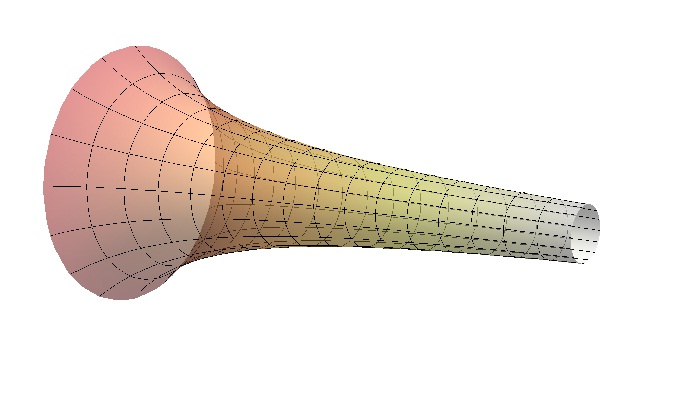
\includegraphics[scale=.5]{Gabriel_Horn}
\subsection{Mathematical Definition}
Gabriel's horn is formed by taking the graph of $y=\frac{1}{x}$, with the domain $x\geq 1$ (thus avoiding the asymptote at $x = 0$) and rotating it in three dimensions about the x-axis. The discovery was made using Cavalieri's principle before the invention of calculus, but today calculus can be used to calculate the volume and surface area of the horn between $x = 1$ and $x = a$, where $a > 1$. Using integration (see Solid of revolution and Surface of revolution for details), it is possible to find the volume $V$ and the surface area $A$:
$$V=\pi\int_1^a \frac{1}{x^2}dx = \pi(1-\frac{1}{a})$$
$$A=2\pi\int_1^a \frac{\sqrt{1+\frac{1}{x^4}}}{x} dx > 2\pi \int_1^a \frac{\sqrt{1}}{x}dx = 2\pi \ln a$$
$a$ can be as large as required, but it can be seen from the equation that the volume of the part of the horn between $x = 1$ and $x = a$ will never exceed $\pi$; however, it will get closer and closer to $\pi$ as $a$ becomes larger. Mathematically, the volume approaches $\pi$ as a approaches infinity. Using the limit notation of calculus, the volume may be expressed as:
$$\lim_{a\to\infty}\pi(1-\frac{1}{a}) = \pi$$
This is so because as $a$ approaches infinity, $\frac{1}{a}$ approaches zero. This means the volume approaches $\pi(1 - 0)$ which equals $\pi$.
As for the area, the above shows that the area is greater than $2\pi$ times the natural logarithm of $a$. There is no upper bound for the natural logarithm of $a$ as it approaches infinity. That means, in this case, that the horn has an infinite surface area. That is to say;
$$2\pi \ln a \to \infty \text{ as } a \to \infty$$
or
$$\lim_{a\to\infty}2\pi\ln a=\infty$$
\subsection{Apparent Paradox}
When the properties of Gabriel's Horn were discovered, the fact that the rotation of an infinite curve about the x-axis generates an object of finite volume was considered paradoxical. However, the explanation is that the bounding curve, $y=\frac{1}{x}$, is simply a special case – just like the simple harmonic series ($\Sigma x^{-1}$) – for which the successive area 'segments' do not decrease rapidly enough to allow for convergence to a limit. For volume segments ($\Sigma \frac{1}{x^2}$) however, and in fact for any generally constructed higher degree curve (eg $y = \frac{1}{x^p}$ where $p>1$), the same is not true and the rate of decrease in the associated series is sufficiently rapid for convergence to a (finite) limiting sum.
The apparent paradox formed part of a great dispute over the nature of infinity involving many of the key thinkers of the time including Thomas Hobbes, John Wallis and Galileo.\footnote{Havil, Julian (2007). \textit{Nonplussed!: mathematical proof of implausible ideas}. Princeton University Press. pp. 82–91. ISBN 0691120560.}
The paradox can also be considered from a non-mathematical perspective. If Gabriel’s Horn existed in reality, it could be filled with a finite amount of paint since it has a finite volume; yet it could never be completely filled, because the first drop would never reach the bottom. But even ignoring this latter consideration, the Horn has an infinite area; so an infinite amount of paint would therefore be required to cover its inner surface: it seems nonsensical to be able to completely fill a space with paint, yet fail to cover all that space's internal surface. The real-world solution to the paradox is that paint is not infinitely divisible; at some point, the throat of the Horn will become too small to allow even a single paint molecule to pass. When considering the Horn to this limited length, the practicably paintable surface of the inner surface is less than the amount of paint needed to fill it to that point. (If paint were infinitely divisible, however, a coat of paint could conceivably have zero thickness, thus making the amount of paint required to cover an infinite surface negligible; and no paradox would result.)\footnote{Clegg, Brian (2003). \textit{Infinity: The Quest to Think the Unthinkable}. Robinson (Constable \& Robinson Ltd). pp. 239-242. ISBN 978-1-84119-650-3.}
\section{Cantor's Set}
\begin{def2}[Cantor's Set]
An example of an uncountable set of measure zero. \\
The Cantor set $T_\infty$, sometimes also called the Cantor comb or no middle third set, is given by taking the interval $[0,1]$ (set $T_0$), removing the open middle third ($T_1$), removing the middle third of each of the two remaining pieces ($T_2$), and continuing this procedure ad infinitum. It is therefore the set of points in the interval $[0,1]$ whose ternary expansions do not contain 1, illustrated above.
Iterating the process $1\to 101, 0 \to 000$ starting with 1 gives the sequence $1, 101, 101000101, 101000101000000000101000101, ...$. The sequence of binary bits thus produced is therefore $1, 0, 1, 0, 0, 0, 1, 0, 1, 0, 0, 0, 0, 0, 0, 0, 0, 0, 1, 0, 1, 0, 0, 0, 1, 0, 1, 0, ...$ whose $n$th term is amazingly given by $D(n,n)=P_n(3)(\mod 3)$, where $D(n,n)$ is a (central) Delannoy number and $P_n(x)$ is a Legendre polynomial \footnote{(E. W. Weisstein, Apr. 9, 2006)}. The recurrence plot for this sequence is illustrated above.
This produces the set of real numbers $\{x\}$ such that
$x=\frac{c_1}{3}+\cdots+\frac{c_n}{3^n}+\cdots$,
where $c_n$ may equal 0 or 2 for each $n$. This is an infinite, perfect set.
\end{def2}
\subsection{The Sierpinski Carpet}
$\begin{array}{c c c c}

\includegraphics[scale=.125]{Seirpinski_Carpet_1} &
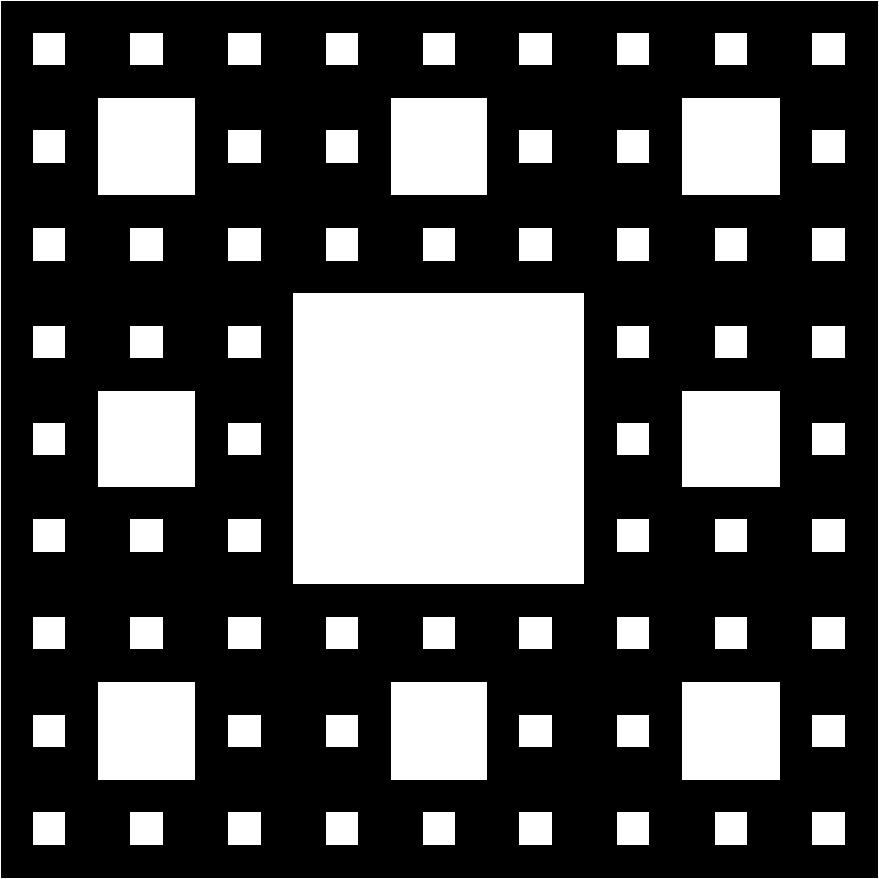
\includegraphics[scale=.125]{Seirpinski_Carpet_3} &
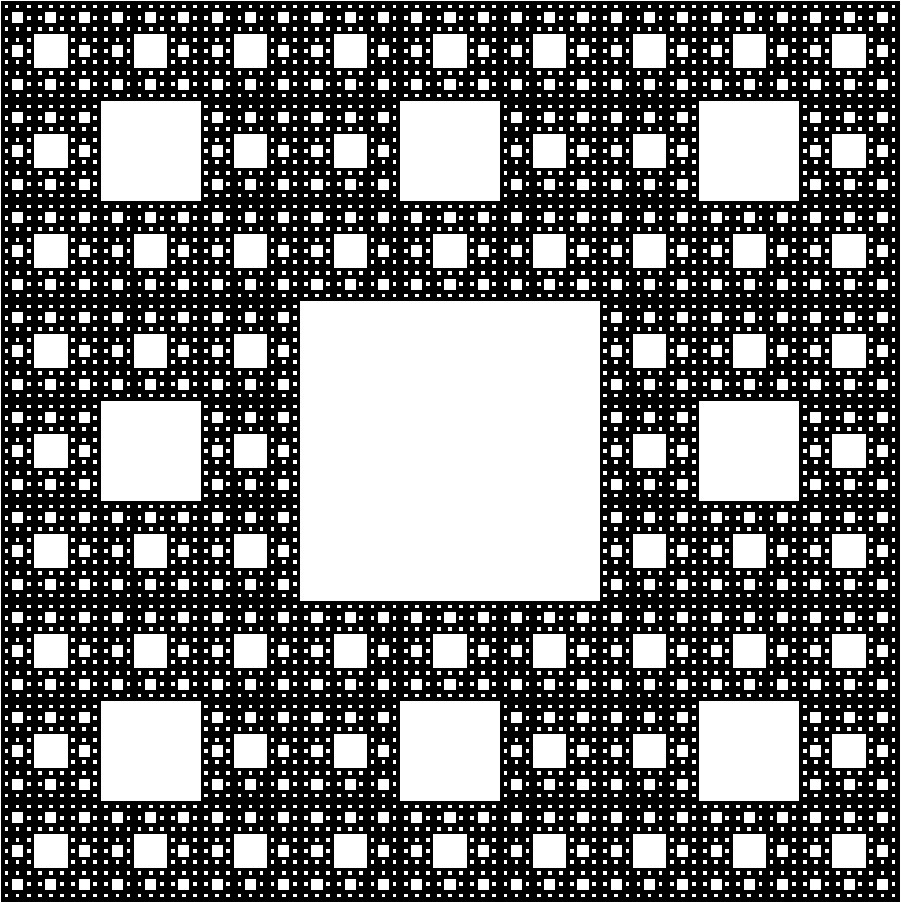
\includegraphics[scale=.125]{Seirpinski_Carpet_5} & 
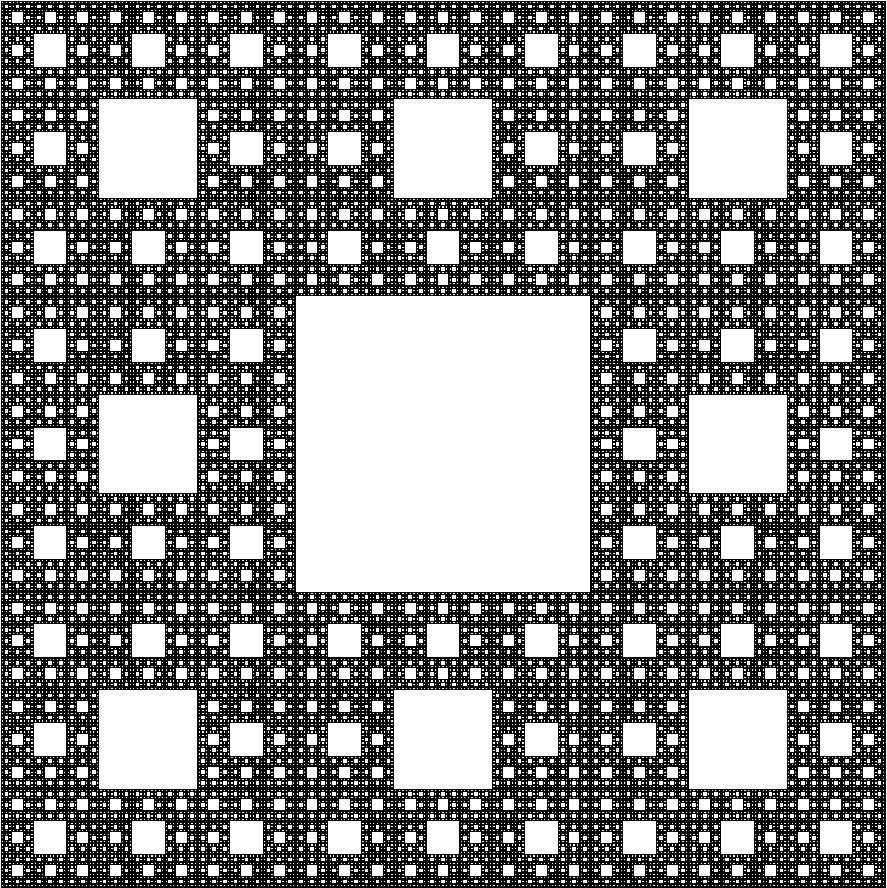
\includegraphics[scale=.125]{Seirpinski_Carpet_7}\\
\end{array}$
\subsection{The Sierpinski Triangle}
$\begin{array}{c c c}
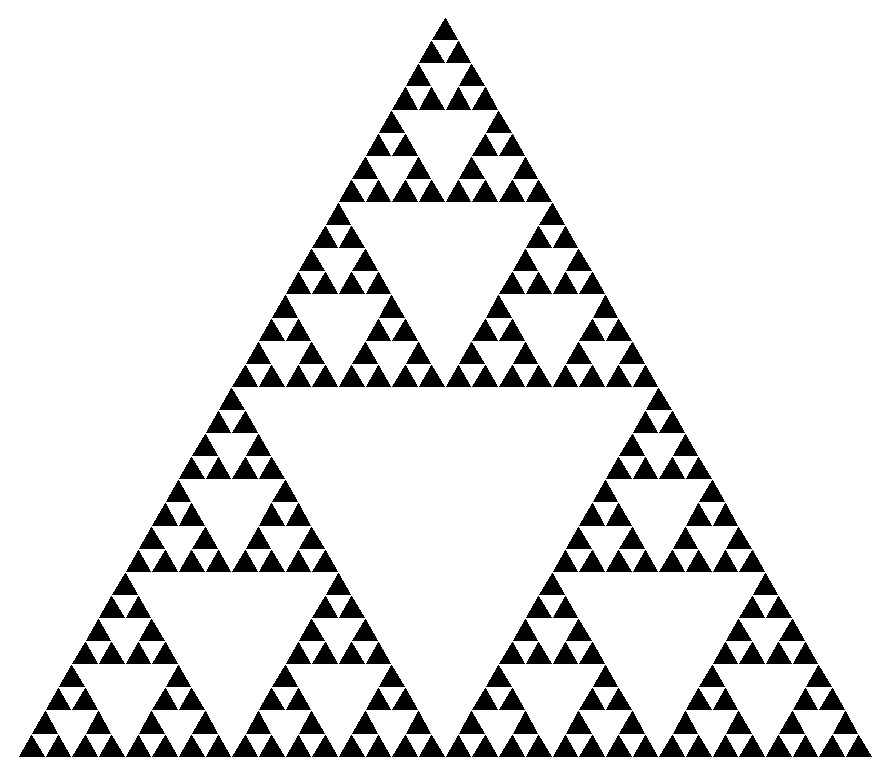
\includegraphics[scale=.125]{Seirpinski_Triangle_5}
\end{array}$
\section{Fun Facts}
\subsection{Thinned-Out Harmonic Series}
You're probably already aware that the harmonic series, which is the sum of the reciprocals of all natural numbers, diverges. In fact, it diverges if you take away every other term. It even diverges if you take away nine out of every ten terms.

So, what do you think would happen if we tried to take the sum of reciprocals of all natural numbers that do not contain the number nine (when written in decimal expansion)?

Amazingly, this series converges!

\textbf{Presentation Suggestions:}
Write out the first several terms. Allow students to guess whether or not this converges. For instance, it may appear that this series is divergent, especially when contrasting it with sums of reciprocals of numbers with one or more $9$'s. That series diverges (easy to show), and this series seems to have "more" terms in it...

\textbf{The Math Behind the Fact:}
Group the terms based on the number of digits in their denominator. There are $8$ terms in $(\frac{1}{1}+...+ \frac{1}{8})$ each of which is no larger than $1$. Consider the next group $(\frac{1}{10}+...+\frac{1}{88})$. The number of terms is at most the number of ways to choose two ordered digits out of the digits $0...8$, and each such term is clearly no larger than $\frac{1}{10}$. So this group's sum is no larger than $\frac{9^2}{10}$. Similarly, the sum of the terms in $(\frac{1}{100}+...+\frac{1}{999})$ is at most $\frac{9^3}{10^2}$, etc.

So the entire sum is no larger than
$9\times 1 + 9\times(\frac{9}{10}) + 9\times(\frac{9^2}{10^2}) + ... + 9\times(\frac{9^n}{10^n}) + ...$

This is a geometric series that converges. Thus by the comparison test, the original sum (which is smaller term-by-term) must converge!
\end{document}
